\documentclass[twoside]{book}

% Packages required by doxygen
\usepackage{fixltx2e}
\usepackage{calc}
\usepackage{doxygen}
\usepackage[export]{adjustbox} % also loads graphicx
\usepackage{graphicx}
\usepackage[utf8]{inputenc}
\usepackage{makeidx}
\usepackage{multicol}
\usepackage{multirow}
\PassOptionsToPackage{warn}{textcomp}
\usepackage{textcomp}
\usepackage[nointegrals]{wasysym}
\usepackage[table]{xcolor}

% Font selection
\usepackage[T1]{fontenc}
\usepackage[scaled=.90]{helvet}
\usepackage{courier}
\usepackage{amssymb}
\usepackage{sectsty}
\renewcommand{\familydefault}{\sfdefault}
\allsectionsfont{%
  \fontseries{bc}\selectfont%
  \color{darkgray}%
}
\renewcommand{\DoxyLabelFont}{%
  \fontseries{bc}\selectfont%
  \color{darkgray}%
}
\newcommand{\+}{\discretionary{\mbox{\scriptsize$\hookleftarrow$}}{}{}}

% Page & text layout
\usepackage{geometry}
\geometry{%
  a4paper,%
  top=2.5cm,%
  bottom=2.5cm,%
  left=2.5cm,%
  right=2.5cm%
}
\tolerance=750
\hfuzz=15pt
\hbadness=750
\setlength{\emergencystretch}{15pt}
\setlength{\parindent}{0cm}
\setlength{\parskip}{3ex plus 2ex minus 2ex}
\makeatletter
\renewcommand{\paragraph}{%
  \@startsection{paragraph}{4}{0ex}{-1.0ex}{1.0ex}{%
    \normalfont\normalsize\bfseries\SS@parafont%
  }%
}
\renewcommand{\subparagraph}{%
  \@startsection{subparagraph}{5}{0ex}{-1.0ex}{1.0ex}{%
    \normalfont\normalsize\bfseries\SS@subparafont%
  }%
}
\makeatother

% Headers & footers
\usepackage{fancyhdr}
\pagestyle{fancyplain}
\fancyhead[LE]{\fancyplain{}{\bfseries\thepage}}
\fancyhead[CE]{\fancyplain{}{}}
\fancyhead[RE]{\fancyplain{}{\bfseries\leftmark}}
\fancyhead[LO]{\fancyplain{}{\bfseries\rightmark}}
\fancyhead[CO]{\fancyplain{}{}}
\fancyhead[RO]{\fancyplain{}{\bfseries\thepage}}
\fancyfoot[LE]{\fancyplain{}{}}
\fancyfoot[CE]{\fancyplain{}{}}
\fancyfoot[RE]{\fancyplain{}{\bfseries\scriptsize Generated by Doxygen }}
\fancyfoot[LO]{\fancyplain{}{\bfseries\scriptsize Generated by Doxygen }}
\fancyfoot[CO]{\fancyplain{}{}}
\fancyfoot[RO]{\fancyplain{}{}}
\renewcommand{\footrulewidth}{0.4pt}
\renewcommand{\chaptermark}[1]{%
  \markboth{#1}{}%
}
\renewcommand{\sectionmark}[1]{%
  \markright{\thesection\ #1}%
}

% Indices & bibliography
\usepackage{natbib}
\usepackage[titles]{tocloft}
\setcounter{tocdepth}{3}
\setcounter{secnumdepth}{5}
\makeindex

% Hyperlinks (required, but should be loaded last)
\usepackage{ifpdf}
\ifpdf
  \usepackage[pdftex,pagebackref=true]{hyperref}
\else
  \usepackage[ps2pdf,pagebackref=true]{hyperref}
\fi
\hypersetup{%
  colorlinks=true,%
  linkcolor=blue,%
  citecolor=blue,%
  unicode%
}

% Custom commands
\newcommand{\clearemptydoublepage}{%
  \newpage{\pagestyle{empty}\cleardoublepage}%
}

\usepackage{caption}
\captionsetup{labelsep=space,justification=centering,font={bf},singlelinecheck=off,skip=4pt,position=top}

%===== C O N T E N T S =====

\begin{document}

% Titlepage & ToC
\hypersetup{pageanchor=false,
             bookmarksnumbered=true,
             pdfencoding=unicode
            }
\pagenumbering{alph}
\begin{titlepage}
\vspace*{7cm}
\begin{center}%
{\Large Tetris M\+I\+N\+IX }\\
\vspace*{1cm}
{\large Generated by Doxygen 1.8.14}\\
\end{center}
\end{titlepage}
\clearemptydoublepage
\pagenumbering{roman}
\tableofcontents
\clearemptydoublepage
\pagenumbering{arabic}
\hypersetup{pageanchor=true}

%--- Begin generated contents ---
\chapter{Module Index}
\section{Modules}
Here is a list of all modules\+:\begin{DoxyCompactList}
\item \contentsline{section}{bitmap}{\pageref{group__bitmap}}{}
\item \contentsline{section}{credits}{\pageref{group__credits}}{}
\item \contentsline{section}{game}{\pageref{group__game}}{}
\item \contentsline{section}{i8042}{\pageref{group__i8042}}{}
\item \contentsline{section}{i8254}{\pageref{group__i8254}}{}
\item \contentsline{section}{kbc}{\pageref{group__kbc}}{}
\item \contentsline{section}{keyboard}{\pageref{group__keyboard}}{}
\item \contentsline{section}{main\+\_\+menu}{\pageref{group__main__menu}}{}
\item \contentsline{section}{mouse}{\pageref{group__mouse}}{}
\item \contentsline{section}{rtc}{\pageref{group__rtc}}{}
\item \contentsline{section}{tetramino}{\pageref{group__tetramino}}{}
\item \contentsline{section}{timer}{\pageref{group__timer}}{}
\item \contentsline{section}{update\+\_\+mov}{\pageref{group__update__mov}}{}
\item \contentsline{section}{vbe}{\pageref{group__vbe}}{}
\item \contentsline{section}{videog}{\pageref{group__videog}}{}
\end{DoxyCompactList}

\chapter{Data Structure Index}
\section{Data Structures}
Here are the data structures with brief descriptions\+:\begin{DoxyCompactList}
\item\contentsline{section}{\mbox{\hyperlink{struct_background}{Background}} }{\pageref{struct_background}}{}
\item\contentsline{section}{\mbox{\hyperlink{struct_bitmap}{Bitmap}} \\*Represents a \mbox{\hyperlink{struct_bitmap}{Bitmap}} }{\pageref{struct_bitmap}}{}
\item\contentsline{section}{\mbox{\hyperlink{struct_bitmap_file_header}{Bitmap\+File\+Header}} }{\pageref{struct_bitmap_file_header}}{}
\item\contentsline{section}{\mbox{\hyperlink{struct_bitmap_info_header}{Bitmap\+Info\+Header}} }{\pageref{struct_bitmap_info_header}}{}
\item\contentsline{section}{\mbox{\hyperlink{struct_board}{Board}} }{\pageref{struct_board}}{}
\item\contentsline{section}{\mbox{\hyperlink{struct_date}{Date}} }{\pageref{struct_date}}{}
\item\contentsline{section}{\mbox{\hyperlink{struct_date__image}{Date\+\_\+image}} }{\pageref{struct_date__image}}{}
\item\contentsline{section}{\mbox{\hyperlink{structgame_over}{game\+Over}} }{\pageref{structgame_over}}{}
\item\contentsline{section}{\mbox{\hyperlink{struct_graphic}{Graphic}} }{\pageref{struct_graphic}}{}
\item\contentsline{section}{\mbox{\hyperlink{structldig}{ldig}} }{\pageref{structldig}}{}
\item\contentsline{section}{\mbox{\hyperlink{structlvl}{lvl}} }{\pageref{structlvl}}{}
\item\contentsline{section}{\mbox{\hyperlink{structpnt}{pnt}} }{\pageref{structpnt}}{}
\item\contentsline{section}{\mbox{\hyperlink{structscoreimg}{scoreimg}} }{\pageref{structscoreimg}}{}
\item\contentsline{section}{\mbox{\hyperlink{struct_square}{Square}} }{\pageref{struct_square}}{}
\item\contentsline{section}{\mbox{\hyperlink{struct_tetramino}{Tetramino}} }{\pageref{struct_tetramino}}{}
\item\contentsline{section}{\mbox{\hyperlink{structtetris}{tetris}} }{\pageref{structtetris}}{}
\end{DoxyCompactList}

\chapter{File Index}
\section{File List}
Here is a list of all files with brief descriptions\+:\begin{DoxyCompactList}
\item\contentsline{section}{C\+:/\+Users/joaom/\+Desktop/\+F\+E\+U\+P/2º ano/\+L\+C\+O\+M/\+M\+I\+N\+I\+X-\/\+L\+C\+O\+M/shared/proj/src/\mbox{\hyperlink{bitmap_8c}{bitmap.\+c}} }{\pageref{bitmap_8c}}{}
\item\contentsline{section}{C\+:/\+Users/joaom/\+Desktop/\+F\+E\+U\+P/2º ano/\+L\+C\+O\+M/\+M\+I\+N\+I\+X-\/\+L\+C\+O\+M/shared/proj/src/\mbox{\hyperlink{bitmap_8h}{bitmap.\+h}} }{\pageref{bitmap_8h}}{}
\item\contentsline{section}{C\+:/\+Users/joaom/\+Desktop/\+F\+E\+U\+P/2º ano/\+L\+C\+O\+M/\+M\+I\+N\+I\+X-\/\+L\+C\+O\+M/shared/proj/src/\mbox{\hyperlink{credits_8c}{credits.\+c}} }{\pageref{credits_8c}}{}
\item\contentsline{section}{C\+:/\+Users/joaom/\+Desktop/\+F\+E\+U\+P/2º ano/\+L\+C\+O\+M/\+M\+I\+N\+I\+X-\/\+L\+C\+O\+M/shared/proj/src/\mbox{\hyperlink{credits_8h}{credits.\+h}} }{\pageref{credits_8h}}{}
\item\contentsline{section}{C\+:/\+Users/joaom/\+Desktop/\+F\+E\+U\+P/2º ano/\+L\+C\+O\+M/\+M\+I\+N\+I\+X-\/\+L\+C\+O\+M/shared/proj/src/\mbox{\hyperlink{game_8c}{game.\+c}} }{\pageref{game_8c}}{}
\item\contentsline{section}{C\+:/\+Users/joaom/\+Desktop/\+F\+E\+U\+P/2º ano/\+L\+C\+O\+M/\+M\+I\+N\+I\+X-\/\+L\+C\+O\+M/shared/proj/src/\mbox{\hyperlink{game_8h}{game.\+h}} }{\pageref{game_8h}}{}
\item\contentsline{section}{C\+:/\+Users/joaom/\+Desktop/\+F\+E\+U\+P/2º ano/\+L\+C\+O\+M/\+M\+I\+N\+I\+X-\/\+L\+C\+O\+M/shared/proj/src/\mbox{\hyperlink{i8042_8h}{i8042.\+h}} }{\pageref{i8042_8h}}{}
\item\contentsline{section}{C\+:/\+Users/joaom/\+Desktop/\+F\+E\+U\+P/2º ano/\+L\+C\+O\+M/\+M\+I\+N\+I\+X-\/\+L\+C\+O\+M/shared/proj/src/\mbox{\hyperlink{i8254_8h}{i8254.\+h}} }{\pageref{i8254_8h}}{}
\item\contentsline{section}{C\+:/\+Users/joaom/\+Desktop/\+F\+E\+U\+P/2º ano/\+L\+C\+O\+M/\+M\+I\+N\+I\+X-\/\+L\+C\+O\+M/shared/proj/src/\mbox{\hyperlink{kbc_8c}{kbc.\+c}} }{\pageref{kbc_8c}}{}
\item\contentsline{section}{C\+:/\+Users/joaom/\+Desktop/\+F\+E\+U\+P/2º ano/\+L\+C\+O\+M/\+M\+I\+N\+I\+X-\/\+L\+C\+O\+M/shared/proj/src/\mbox{\hyperlink{kbc_8h}{kbc.\+h}} }{\pageref{kbc_8h}}{}
\item\contentsline{section}{C\+:/\+Users/joaom/\+Desktop/\+F\+E\+U\+P/2º ano/\+L\+C\+O\+M/\+M\+I\+N\+I\+X-\/\+L\+C\+O\+M/shared/proj/src/\mbox{\hyperlink{keyboard_8c}{keyboard.\+c}} }{\pageref{keyboard_8c}}{}
\item\contentsline{section}{C\+:/\+Users/joaom/\+Desktop/\+F\+E\+U\+P/2º ano/\+L\+C\+O\+M/\+M\+I\+N\+I\+X-\/\+L\+C\+O\+M/shared/proj/src/\mbox{\hyperlink{keyboard_8h}{keyboard.\+h}} }{\pageref{keyboard_8h}}{}
\item\contentsline{section}{C\+:/\+Users/joaom/\+Desktop/\+F\+E\+U\+P/2º ano/\+L\+C\+O\+M/\+M\+I\+N\+I\+X-\/\+L\+C\+O\+M/shared/proj/src/\mbox{\hyperlink{main__menu_8c}{main\+\_\+menu.\+c}} }{\pageref{main__menu_8c}}{}
\item\contentsline{section}{C\+:/\+Users/joaom/\+Desktop/\+F\+E\+U\+P/2º ano/\+L\+C\+O\+M/\+M\+I\+N\+I\+X-\/\+L\+C\+O\+M/shared/proj/src/\mbox{\hyperlink{main__menu_8h}{main\+\_\+menu.\+h}} }{\pageref{main__menu_8h}}{}
\item\contentsline{section}{C\+:/\+Users/joaom/\+Desktop/\+F\+E\+U\+P/2º ano/\+L\+C\+O\+M/\+M\+I\+N\+I\+X-\/\+L\+C\+O\+M/shared/proj/src/\mbox{\hyperlink{mouse_8c}{mouse.\+c}} }{\pageref{mouse_8c}}{}
\item\contentsline{section}{C\+:/\+Users/joaom/\+Desktop/\+F\+E\+U\+P/2º ano/\+L\+C\+O\+M/\+M\+I\+N\+I\+X-\/\+L\+C\+O\+M/shared/proj/src/\mbox{\hyperlink{mouse_8h}{mouse.\+h}} }{\pageref{mouse_8h}}{}
\item\contentsline{section}{C\+:/\+Users/joaom/\+Desktop/\+F\+E\+U\+P/2º ano/\+L\+C\+O\+M/\+M\+I\+N\+I\+X-\/\+L\+C\+O\+M/shared/proj/src/\mbox{\hyperlink{proj_8c}{proj.\+c}} }{\pageref{proj_8c}}{}
\item\contentsline{section}{C\+:/\+Users/joaom/\+Desktop/\+F\+E\+U\+P/2º ano/\+L\+C\+O\+M/\+M\+I\+N\+I\+X-\/\+L\+C\+O\+M/shared/proj/src/\mbox{\hyperlink{rtc_8c}{rtc.\+c}} }{\pageref{rtc_8c}}{}
\item\contentsline{section}{C\+:/\+Users/joaom/\+Desktop/\+F\+E\+U\+P/2º ano/\+L\+C\+O\+M/\+M\+I\+N\+I\+X-\/\+L\+C\+O\+M/shared/proj/src/\mbox{\hyperlink{rtc_8h}{rtc.\+h}} }{\pageref{rtc_8h}}{}
\item\contentsline{section}{C\+:/\+Users/joaom/\+Desktop/\+F\+E\+U\+P/2º ano/\+L\+C\+O\+M/\+M\+I\+N\+I\+X-\/\+L\+C\+O\+M/shared/proj/src/\mbox{\hyperlink{tetromino_8c}{tetromino.\+c}} }{\pageref{tetromino_8c}}{}
\item\contentsline{section}{C\+:/\+Users/joaom/\+Desktop/\+F\+E\+U\+P/2º ano/\+L\+C\+O\+M/\+M\+I\+N\+I\+X-\/\+L\+C\+O\+M/shared/proj/src/\mbox{\hyperlink{tetromino_8h}{tetromino.\+h}} }{\pageref{tetromino_8h}}{}
\item\contentsline{section}{C\+:/\+Users/joaom/\+Desktop/\+F\+E\+U\+P/2º ano/\+L\+C\+O\+M/\+M\+I\+N\+I\+X-\/\+L\+C\+O\+M/shared/proj/src/\mbox{\hyperlink{timer_8c}{timer.\+c}} }{\pageref{timer_8c}}{}
\item\contentsline{section}{C\+:/\+Users/joaom/\+Desktop/\+F\+E\+U\+P/2º ano/\+L\+C\+O\+M/\+M\+I\+N\+I\+X-\/\+L\+C\+O\+M/shared/proj/src/\mbox{\hyperlink{timer_8h}{timer.\+h}} }{\pageref{timer_8h}}{}
\item\contentsline{section}{C\+:/\+Users/joaom/\+Desktop/\+F\+E\+U\+P/2º ano/\+L\+C\+O\+M/\+M\+I\+N\+I\+X-\/\+L\+C\+O\+M/shared/proj/src/\mbox{\hyperlink{update__mov_8c}{update\+\_\+mov.\+c}} }{\pageref{update__mov_8c}}{}
\item\contentsline{section}{C\+:/\+Users/joaom/\+Desktop/\+F\+E\+U\+P/2º ano/\+L\+C\+O\+M/\+M\+I\+N\+I\+X-\/\+L\+C\+O\+M/shared/proj/src/\mbox{\hyperlink{update__mov_8h}{update\+\_\+mov.\+h}} }{\pageref{update__mov_8h}}{}
\item\contentsline{section}{C\+:/\+Users/joaom/\+Desktop/\+F\+E\+U\+P/2º ano/\+L\+C\+O\+M/\+M\+I\+N\+I\+X-\/\+L\+C\+O\+M/shared/proj/src/\mbox{\hyperlink{vbe_8c}{vbe.\+c}} }{\pageref{vbe_8c}}{}
\item\contentsline{section}{C\+:/\+Users/joaom/\+Desktop/\+F\+E\+U\+P/2º ano/\+L\+C\+O\+M/\+M\+I\+N\+I\+X-\/\+L\+C\+O\+M/shared/proj/src/\mbox{\hyperlink{vbe_8h}{vbe.\+h}} }{\pageref{vbe_8h}}{}
\item\contentsline{section}{C\+:/\+Users/joaom/\+Desktop/\+F\+E\+U\+P/2º ano/\+L\+C\+O\+M/\+M\+I\+N\+I\+X-\/\+L\+C\+O\+M/shared/proj/src/\mbox{\hyperlink{videog_8c}{videog.\+c}} }{\pageref{videog_8c}}{}
\item\contentsline{section}{C\+:/\+Users/joaom/\+Desktop/\+F\+E\+U\+P/2º ano/\+L\+C\+O\+M/\+M\+I\+N\+I\+X-\/\+L\+C\+O\+M/shared/proj/src/\mbox{\hyperlink{videog_8h}{videog.\+h}} }{\pageref{videog_8h}}{}
\end{DoxyCompactList}

\chapter{Module Documentation}
\hypertarget{group__bitmap}{}\section{bitmap}
\label{group__bitmap}\index{bitmap@{bitmap}}
\subsection*{Data Structures}
\begin{DoxyCompactItemize}
\item 
struct \mbox{\hyperlink{struct_bitmap_file_header}{Bitmap\+File\+Header}}
\item 
struct \mbox{\hyperlink{struct_bitmap_info_header}{Bitmap\+Info\+Header}}
\item 
struct \mbox{\hyperlink{struct_bitmap}{Bitmap}}
\begin{DoxyCompactList}\small\item\em Represents a \mbox{\hyperlink{struct_bitmap}{Bitmap}}. \end{DoxyCompactList}\end{DoxyCompactItemize}
\subsection*{Enumerations}
\begin{DoxyCompactItemize}
\item 
enum \mbox{\hyperlink{group__bitmap_gacdfaca60ec19c0265bac2692d7982726}{Alignment}} \{ \mbox{\hyperlink{group__bitmap_ggacdfaca60ec19c0265bac2692d7982726a6ec599857e15466988726932dd592305}{A\+L\+I\+G\+N\+\_\+\+L\+E\+FT}}, 
\mbox{\hyperlink{group__bitmap_ggacdfaca60ec19c0265bac2692d7982726a5624165187e56db612253e608a45b1c6}{A\+L\+I\+G\+N\+\_\+\+C\+E\+N\+T\+ER}}, 
\mbox{\hyperlink{group__bitmap_ggacdfaca60ec19c0265bac2692d7982726a9c81840e8cad46418b39a8b74a246354}{A\+L\+I\+G\+N\+\_\+\+R\+I\+G\+HT}}
 \}
\end{DoxyCompactItemize}
\subsection*{Functions}
\begin{DoxyCompactItemize}
\item 
\mbox{\hyperlink{struct_bitmap}{Bitmap}} $\ast$ \mbox{\hyperlink{group__bitmap_ga3506880ffd407c36eb8aaddd2c1606d2}{load\+Bitmap}} (const char $\ast$filename)
\begin{DoxyCompactList}\small\item\em Loads a bmp image. \end{DoxyCompactList}\item 
void \mbox{\hyperlink{group__bitmap_ga6652acd82369d03df807a689437efc1b}{draw\+Bitmap}} (\mbox{\hyperlink{struct_bitmap}{Bitmap}} $\ast$bmp, int x, int y, \mbox{\hyperlink{group__bitmap_gacdfaca60ec19c0265bac2692d7982726}{Alignment}} alignment)
\begin{DoxyCompactList}\small\item\em Draws an unscaled, unrotated bitmap at the given position. \end{DoxyCompactList}\item 
void \mbox{\hyperlink{group__bitmap_ga08c1d4f4fff81df260d979ea8fc1aa61}{delete\+Bitmap}} (\mbox{\hyperlink{struct_bitmap}{Bitmap}} $\ast$bmp)
\begin{DoxyCompactList}\small\item\em Destroys the given bitmap, freeing all resources used by it. \end{DoxyCompactList}\end{DoxyCompactItemize}
\subsection*{Variables}
\begin{DoxyCompactItemize}
\item 
unsigned short \mbox{\hyperlink{group__bitmap_gaa929142c5ddf34cf0915c97a617a1a63}{type}}
\item 
unsigned int \mbox{\hyperlink{group__bitmap_gaac913b3a1f6ef005d66bf7a84428773e}{size}}
\item 
unsigned int \mbox{\hyperlink{group__bitmap_ga05d5cbcb44f437341bd9fa37d589aced}{reserved}}
\item 
unsigned int \mbox{\hyperlink{group__bitmap_ga29b5297d3393519050e3126c4cb07c1c}{offset}}
\item 
unsigned int \mbox{\hyperlink{group__bitmap_gaac913b3a1f6ef005d66bf7a84428773e}{size}}
\item 
int \mbox{\hyperlink{group__bitmap_ga2474a5474cbff19523a51eb1de01cda4}{width}}
\item 
int \mbox{\hyperlink{group__bitmap_gad12fc34ce789bce6c8a05d8a17138534}{height}}
\item 
unsigned short \mbox{\hyperlink{group__bitmap_ga8c89d091e05544a82dc2398eed99634f}{planes}}
\item 
unsigned short \mbox{\hyperlink{group__bitmap_ga47d1d4d776f8fd3bb0f7dbc3c5aeb534}{bits}}
\item 
unsigned int \mbox{\hyperlink{group__bitmap_gad180079f62b44e49ec672c9ef6e078b3}{compression}}
\item 
unsigned int \mbox{\hyperlink{group__bitmap_gadcd57a0168319e747bc8099218d3822c}{image\+Size}}
\item 
int \mbox{\hyperlink{group__bitmap_gac6eaeb4c0876cf6cd899f41fe3c25ff5}{x\+Resolution}}
\item 
int \mbox{\hyperlink{group__bitmap_gaa2f350dd0bda750656d5db5f5e37b2b3}{y\+Resolution}}
\item 
unsigned int \mbox{\hyperlink{group__bitmap_gaed4506bad904845183194f199f1bdb98}{n\+Colors}}
\item 
unsigned int \mbox{\hyperlink{group__bitmap_ga8f7abfbc446b12f385d2b42c3b4fd9b0}{important\+Colors}}
\item 
\mbox{\hyperlink{struct_bitmap_info_header}{Bitmap\+Info\+Header}} \mbox{\hyperlink{group__bitmap_ga7157ca7f3ce4be47481c472fafd89313}{bitmap\+Info\+Header}}
\item 
char $\ast$ \mbox{\hyperlink{group__bitmap_ga212b0ad51a5ac5d020dcf840678ef146}{bitmap\+Data}}
\end{DoxyCompactItemize}


\subsection{Detailed Description}
Functions for using the bitmap loader 

\subsection{Enumeration Type Documentation}
\mbox{\Hypertarget{group__bitmap_gacdfaca60ec19c0265bac2692d7982726}\label{group__bitmap_gacdfaca60ec19c0265bac2692d7982726}} 
\index{bitmap@{bitmap}!Alignment@{Alignment}}
\index{Alignment@{Alignment}!bitmap@{bitmap}}
\subsubsection{\texorpdfstring{Alignment}{Alignment}}
{\footnotesize\ttfamily enum \mbox{\hyperlink{group__bitmap_gacdfaca60ec19c0265bac2692d7982726}{Alignment}}}

\begin{DoxyEnumFields}{Enumerator}
\raisebox{\heightof{T}}[0pt][0pt]{\index{A\+L\+I\+G\+N\+\_\+\+L\+E\+FT@{A\+L\+I\+G\+N\+\_\+\+L\+E\+FT}!bitmap@{bitmap}}\index{bitmap@{bitmap}!A\+L\+I\+G\+N\+\_\+\+L\+E\+FT@{A\+L\+I\+G\+N\+\_\+\+L\+E\+FT}}}\mbox{\Hypertarget{group__bitmap_ggacdfaca60ec19c0265bac2692d7982726a6ec599857e15466988726932dd592305}\label{group__bitmap_ggacdfaca60ec19c0265bac2692d7982726a6ec599857e15466988726932dd592305}} 
A\+L\+I\+G\+N\+\_\+\+L\+E\+FT&\\
\hline

\raisebox{\heightof{T}}[0pt][0pt]{\index{A\+L\+I\+G\+N\+\_\+\+C\+E\+N\+T\+ER@{A\+L\+I\+G\+N\+\_\+\+C\+E\+N\+T\+ER}!bitmap@{bitmap}}\index{bitmap@{bitmap}!A\+L\+I\+G\+N\+\_\+\+C\+E\+N\+T\+ER@{A\+L\+I\+G\+N\+\_\+\+C\+E\+N\+T\+ER}}}\mbox{\Hypertarget{group__bitmap_ggacdfaca60ec19c0265bac2692d7982726a5624165187e56db612253e608a45b1c6}\label{group__bitmap_ggacdfaca60ec19c0265bac2692d7982726a5624165187e56db612253e608a45b1c6}} 
A\+L\+I\+G\+N\+\_\+\+C\+E\+N\+T\+ER&\\
\hline

\raisebox{\heightof{T}}[0pt][0pt]{\index{A\+L\+I\+G\+N\+\_\+\+R\+I\+G\+HT@{A\+L\+I\+G\+N\+\_\+\+R\+I\+G\+HT}!bitmap@{bitmap}}\index{bitmap@{bitmap}!A\+L\+I\+G\+N\+\_\+\+R\+I\+G\+HT@{A\+L\+I\+G\+N\+\_\+\+R\+I\+G\+HT}}}\mbox{\Hypertarget{group__bitmap_ggacdfaca60ec19c0265bac2692d7982726a9c81840e8cad46418b39a8b74a246354}\label{group__bitmap_ggacdfaca60ec19c0265bac2692d7982726a9c81840e8cad46418b39a8b74a246354}} 
A\+L\+I\+G\+N\+\_\+\+R\+I\+G\+HT&\\
\hline

\end{DoxyEnumFields}


\subsection{Function Documentation}
\mbox{\Hypertarget{group__bitmap_ga08c1d4f4fff81df260d979ea8fc1aa61}\label{group__bitmap_ga08c1d4f4fff81df260d979ea8fc1aa61}} 
\index{bitmap@{bitmap}!delete\+Bitmap@{delete\+Bitmap}}
\index{delete\+Bitmap@{delete\+Bitmap}!bitmap@{bitmap}}
\subsubsection{\texorpdfstring{delete\+Bitmap()}{deleteBitmap()}}
{\footnotesize\ttfamily void delete\+Bitmap (\begin{DoxyParamCaption}\item[{\mbox{\hyperlink{struct_bitmap}{Bitmap}} $\ast$}]{bmp }\end{DoxyParamCaption})}



Destroys the given bitmap, freeing all resources used by it. 


\begin{DoxyParams}{Parameters}
{\em bitmap} & bitmap to be destroyed \\
\hline
\end{DoxyParams}
Here is the caller graph for this function\+:
\nopagebreak
\begin{figure}[H]
\begin{center}
\leavevmode
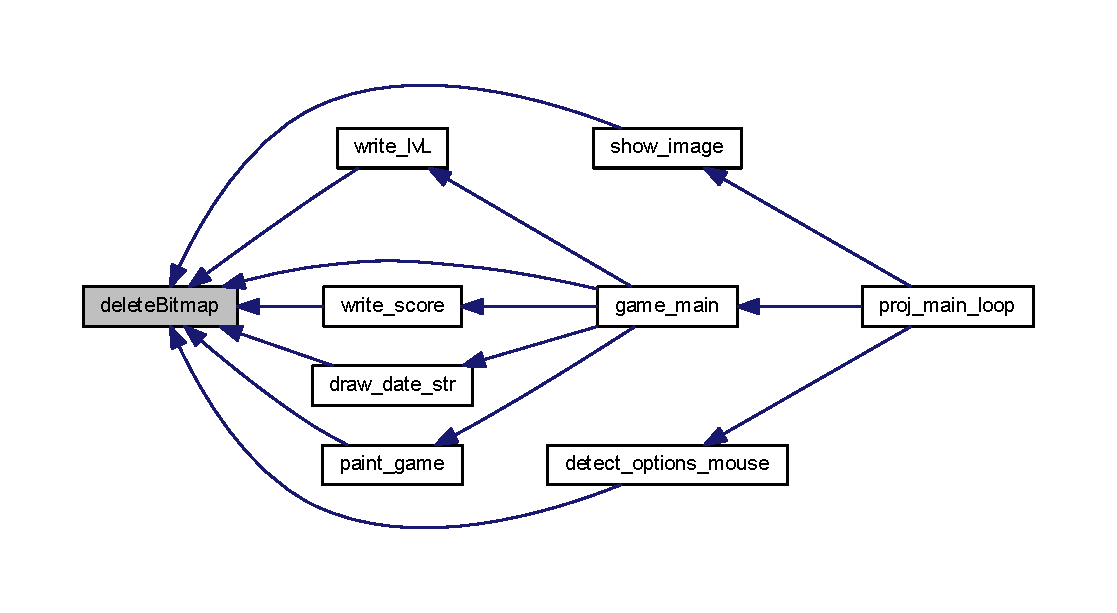
\includegraphics[width=350pt]{group__bitmap_ga08c1d4f4fff81df260d979ea8fc1aa61_icgraph}
\end{center}
\end{figure}
\mbox{\Hypertarget{group__bitmap_ga6652acd82369d03df807a689437efc1b}\label{group__bitmap_ga6652acd82369d03df807a689437efc1b}} 
\index{bitmap@{bitmap}!draw\+Bitmap@{draw\+Bitmap}}
\index{draw\+Bitmap@{draw\+Bitmap}!bitmap@{bitmap}}
\subsubsection{\texorpdfstring{draw\+Bitmap()}{drawBitmap()}}
{\footnotesize\ttfamily void draw\+Bitmap (\begin{DoxyParamCaption}\item[{\mbox{\hyperlink{struct_bitmap}{Bitmap}} $\ast$}]{bmp,  }\item[{int}]{x,  }\item[{int}]{y,  }\item[{\mbox{\hyperlink{group__bitmap_gacdfaca60ec19c0265bac2692d7982726}{Alignment}}}]{alignment }\end{DoxyParamCaption})}



Draws an unscaled, unrotated bitmap at the given position. 


\begin{DoxyParams}{Parameters}
{\em bitmap} & bitmap to be drawn \\
\hline
{\em x} & destiny x coord \\
\hline
{\em y} & destiny y coord \\
\hline
{\em alignment} & image alignment \\
\hline
\end{DoxyParams}
Here is the call graph for this function\+:
\nopagebreak
\begin{figure}[H]
\begin{center}
\leavevmode
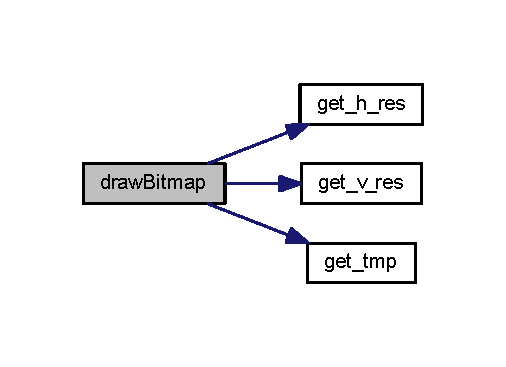
\includegraphics[width=243pt]{group__bitmap_ga6652acd82369d03df807a689437efc1b_cgraph}
\end{center}
\end{figure}
Here is the caller graph for this function\+:
\nopagebreak
\begin{figure}[H]
\begin{center}
\leavevmode
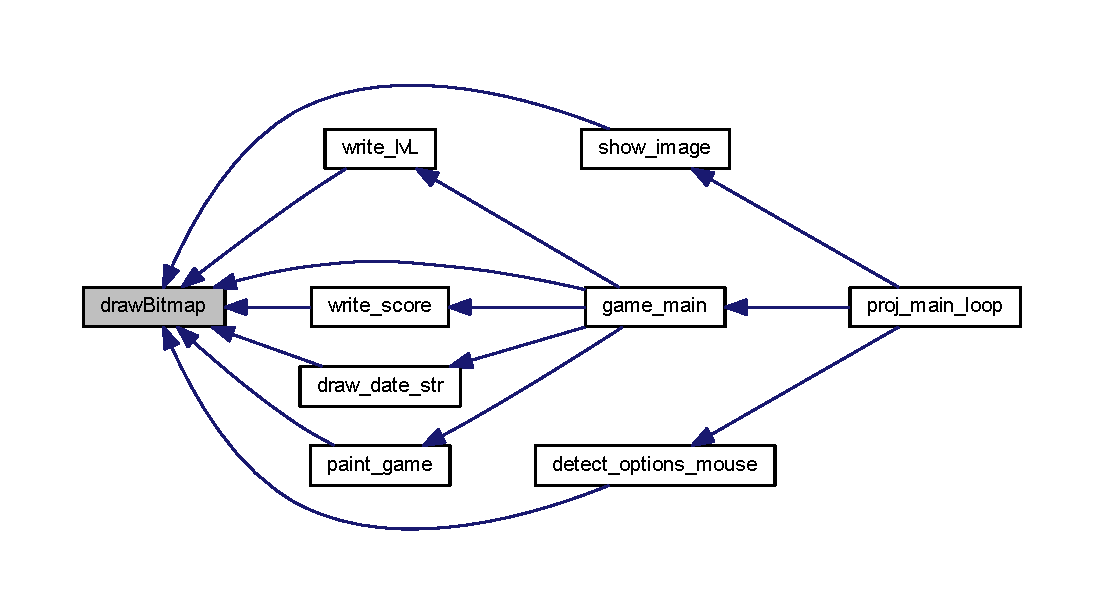
\includegraphics[width=350pt]{group__bitmap_ga6652acd82369d03df807a689437efc1b_icgraph}
\end{center}
\end{figure}
\mbox{\Hypertarget{group__bitmap_ga3506880ffd407c36eb8aaddd2c1606d2}\label{group__bitmap_ga3506880ffd407c36eb8aaddd2c1606d2}} 
\index{bitmap@{bitmap}!load\+Bitmap@{load\+Bitmap}}
\index{load\+Bitmap@{load\+Bitmap}!bitmap@{bitmap}}
\subsubsection{\texorpdfstring{load\+Bitmap()}{loadBitmap()}}
{\footnotesize\ttfamily \mbox{\hyperlink{struct_bitmap}{Bitmap}}$\ast$ load\+Bitmap (\begin{DoxyParamCaption}\item[{const char $\ast$}]{filename }\end{DoxyParamCaption})}



Loads a bmp image. 


\begin{DoxyParams}{Parameters}
{\em filename} & Path of the image to load \\
\hline
\end{DoxyParams}
\begin{DoxyReturn}{Returns}
Non N\+U\+LL pointer to the image buffer 
\end{DoxyReturn}
Here is the caller graph for this function\+:
\nopagebreak
\begin{figure}[H]
\begin{center}
\leavevmode
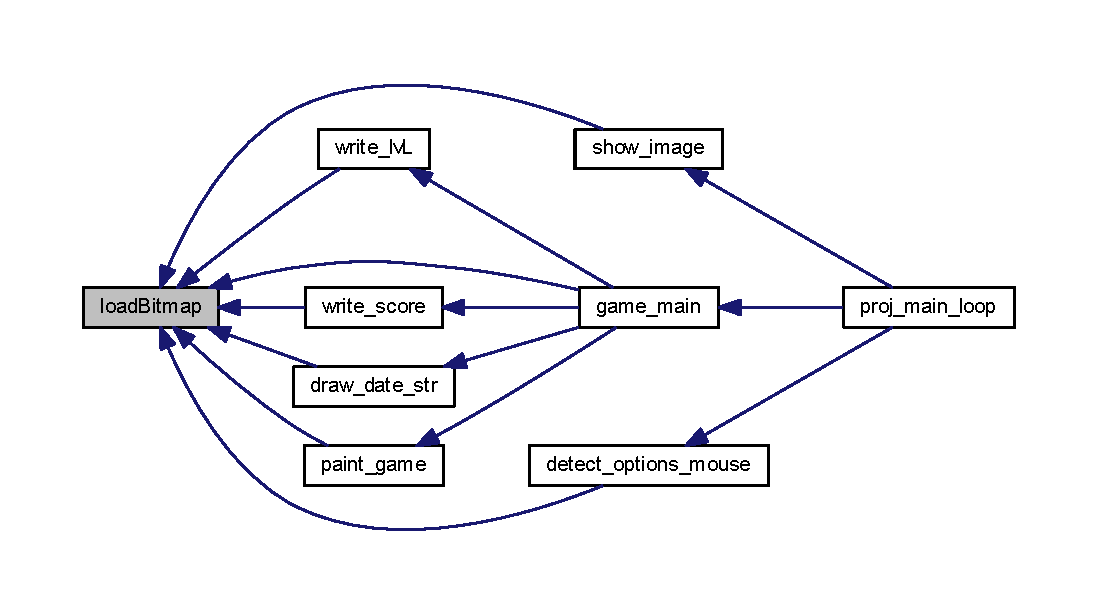
\includegraphics[width=350pt]{group__bitmap_ga3506880ffd407c36eb8aaddd2c1606d2_icgraph}
\end{center}
\end{figure}


\subsection{Variable Documentation}
\mbox{\Hypertarget{group__bitmap_ga212b0ad51a5ac5d020dcf840678ef146}\label{group__bitmap_ga212b0ad51a5ac5d020dcf840678ef146}} 
\index{bitmap@{bitmap}!bitmap\+Data@{bitmap\+Data}}
\index{bitmap\+Data@{bitmap\+Data}!bitmap@{bitmap}}
\subsubsection{\texorpdfstring{bitmap\+Data}{bitmapData}}
{\footnotesize\ttfamily char$\ast$ bitmap\+Data}

\mbox{\Hypertarget{group__bitmap_ga7157ca7f3ce4be47481c472fafd89313}\label{group__bitmap_ga7157ca7f3ce4be47481c472fafd89313}} 
\index{bitmap@{bitmap}!bitmap\+Info\+Header@{bitmap\+Info\+Header}}
\index{bitmap\+Info\+Header@{bitmap\+Info\+Header}!bitmap@{bitmap}}
\subsubsection{\texorpdfstring{bitmap\+Info\+Header}{bitmapInfoHeader}}
{\footnotesize\ttfamily \mbox{\hyperlink{struct_bitmap_info_header}{Bitmap\+Info\+Header}} bitmap\+Info\+Header}

\mbox{\Hypertarget{group__bitmap_ga47d1d4d776f8fd3bb0f7dbc3c5aeb534}\label{group__bitmap_ga47d1d4d776f8fd3bb0f7dbc3c5aeb534}} 
\index{bitmap@{bitmap}!bits@{bits}}
\index{bits@{bits}!bitmap@{bitmap}}
\subsubsection{\texorpdfstring{bits}{bits}}
{\footnotesize\ttfamily unsigned short bits}

\mbox{\Hypertarget{group__bitmap_gad180079f62b44e49ec672c9ef6e078b3}\label{group__bitmap_gad180079f62b44e49ec672c9ef6e078b3}} 
\index{bitmap@{bitmap}!compression@{compression}}
\index{compression@{compression}!bitmap@{bitmap}}
\subsubsection{\texorpdfstring{compression}{compression}}
{\footnotesize\ttfamily unsigned int compression}

\mbox{\Hypertarget{group__bitmap_gad12fc34ce789bce6c8a05d8a17138534}\label{group__bitmap_gad12fc34ce789bce6c8a05d8a17138534}} 
\index{bitmap@{bitmap}!height@{height}}
\index{height@{height}!bitmap@{bitmap}}
\subsubsection{\texorpdfstring{height}{height}}
{\footnotesize\ttfamily int height}

\mbox{\Hypertarget{group__bitmap_gadcd57a0168319e747bc8099218d3822c}\label{group__bitmap_gadcd57a0168319e747bc8099218d3822c}} 
\index{bitmap@{bitmap}!image\+Size@{image\+Size}}
\index{image\+Size@{image\+Size}!bitmap@{bitmap}}
\subsubsection{\texorpdfstring{image\+Size}{imageSize}}
{\footnotesize\ttfamily unsigned int image\+Size}

\mbox{\Hypertarget{group__bitmap_ga8f7abfbc446b12f385d2b42c3b4fd9b0}\label{group__bitmap_ga8f7abfbc446b12f385d2b42c3b4fd9b0}} 
\index{bitmap@{bitmap}!important\+Colors@{important\+Colors}}
\index{important\+Colors@{important\+Colors}!bitmap@{bitmap}}
\subsubsection{\texorpdfstring{important\+Colors}{importantColors}}
{\footnotesize\ttfamily unsigned int important\+Colors}

\mbox{\Hypertarget{group__bitmap_gaed4506bad904845183194f199f1bdb98}\label{group__bitmap_gaed4506bad904845183194f199f1bdb98}} 
\index{bitmap@{bitmap}!n\+Colors@{n\+Colors}}
\index{n\+Colors@{n\+Colors}!bitmap@{bitmap}}
\subsubsection{\texorpdfstring{n\+Colors}{nColors}}
{\footnotesize\ttfamily unsigned int n\+Colors}

\mbox{\Hypertarget{group__bitmap_ga29b5297d3393519050e3126c4cb07c1c}\label{group__bitmap_ga29b5297d3393519050e3126c4cb07c1c}} 
\index{bitmap@{bitmap}!offset@{offset}}
\index{offset@{offset}!bitmap@{bitmap}}
\subsubsection{\texorpdfstring{offset}{offset}}
{\footnotesize\ttfamily unsigned int offset}

\mbox{\Hypertarget{group__bitmap_ga8c89d091e05544a82dc2398eed99634f}\label{group__bitmap_ga8c89d091e05544a82dc2398eed99634f}} 
\index{bitmap@{bitmap}!planes@{planes}}
\index{planes@{planes}!bitmap@{bitmap}}
\subsubsection{\texorpdfstring{planes}{planes}}
{\footnotesize\ttfamily unsigned short planes}

\mbox{\Hypertarget{group__bitmap_ga05d5cbcb44f437341bd9fa37d589aced}\label{group__bitmap_ga05d5cbcb44f437341bd9fa37d589aced}} 
\index{bitmap@{bitmap}!reserved@{reserved}}
\index{reserved@{reserved}!bitmap@{bitmap}}
\subsubsection{\texorpdfstring{reserved}{reserved}}
{\footnotesize\ttfamily unsigned int reserved}

\mbox{\Hypertarget{group__bitmap_gaac913b3a1f6ef005d66bf7a84428773e}\label{group__bitmap_gaac913b3a1f6ef005d66bf7a84428773e}} 
\index{bitmap@{bitmap}!size@{size}}
\index{size@{size}!bitmap@{bitmap}}
\subsubsection{\texorpdfstring{size}{size}\hspace{0.1cm}{\footnotesize\ttfamily [1/2]}}
{\footnotesize\ttfamily unsigned int size}

\mbox{\Hypertarget{group__bitmap_gaac913b3a1f6ef005d66bf7a84428773e}\label{group__bitmap_gaac913b3a1f6ef005d66bf7a84428773e}} 
\index{bitmap@{bitmap}!size@{size}}
\index{size@{size}!bitmap@{bitmap}}
\subsubsection{\texorpdfstring{size}{size}\hspace{0.1cm}{\footnotesize\ttfamily [2/2]}}
{\footnotesize\ttfamily unsigned int size}

\mbox{\Hypertarget{group__bitmap_gaa929142c5ddf34cf0915c97a617a1a63}\label{group__bitmap_gaa929142c5ddf34cf0915c97a617a1a63}} 
\index{bitmap@{bitmap}!type@{type}}
\index{type@{type}!bitmap@{bitmap}}
\subsubsection{\texorpdfstring{type}{type}}
{\footnotesize\ttfamily unsigned short type}

\mbox{\Hypertarget{group__bitmap_ga2474a5474cbff19523a51eb1de01cda4}\label{group__bitmap_ga2474a5474cbff19523a51eb1de01cda4}} 
\index{bitmap@{bitmap}!width@{width}}
\index{width@{width}!bitmap@{bitmap}}
\subsubsection{\texorpdfstring{width}{width}}
{\footnotesize\ttfamily int width}

\mbox{\Hypertarget{group__bitmap_gac6eaeb4c0876cf6cd899f41fe3c25ff5}\label{group__bitmap_gac6eaeb4c0876cf6cd899f41fe3c25ff5}} 
\index{bitmap@{bitmap}!x\+Resolution@{x\+Resolution}}
\index{x\+Resolution@{x\+Resolution}!bitmap@{bitmap}}
\subsubsection{\texorpdfstring{x\+Resolution}{xResolution}}
{\footnotesize\ttfamily int x\+Resolution}

\mbox{\Hypertarget{group__bitmap_gaa2f350dd0bda750656d5db5f5e37b2b3}\label{group__bitmap_gaa2f350dd0bda750656d5db5f5e37b2b3}} 
\index{bitmap@{bitmap}!y\+Resolution@{y\+Resolution}}
\index{y\+Resolution@{y\+Resolution}!bitmap@{bitmap}}
\subsubsection{\texorpdfstring{y\+Resolution}{yResolution}}
{\footnotesize\ttfamily int y\+Resolution}


\hypertarget{group__credits}{}\section{credits}
\label{group__credits}\index{credits@{credits}}
\subsection*{Data Structures}
\begin{DoxyCompactItemize}
\item 
struct \mbox{\hyperlink{struct_graphic}{Graphic}}
\end{DoxyCompactItemize}
\subsection*{Functions}
\begin{DoxyCompactItemize}
\item 
int \mbox{\hyperlink{group__credits_ga2d90e43cf8b9ee19d3dca31eb1c9cddd}{show\+\_\+image}} ()
\begin{DoxyCompactList}\small\item\em Presents Credits to user while E\+SC key isn\textquotesingle{}t pressed. \end{DoxyCompactList}\end{DoxyCompactItemize}
\subsection*{Variables}
\begin{DoxyCompactItemize}
\item 
\mbox{\hyperlink{struct_bitmap}{Bitmap}} $\ast$ \mbox{\hyperlink{group__credits_ga801bef0ab9d72c95bc5d6d6a0d8f2db0}{image}}
\end{DoxyCompactItemize}


\subsection{Detailed Description}
Functions to handle the credits event 

\subsection{Function Documentation}
\mbox{\Hypertarget{group__credits_ga2d90e43cf8b9ee19d3dca31eb1c9cddd}\label{group__credits_ga2d90e43cf8b9ee19d3dca31eb1c9cddd}} 
\index{credits@{credits}!show\+\_\+image@{show\+\_\+image}}
\index{show\+\_\+image@{show\+\_\+image}!credits@{credits}}
\subsubsection{\texorpdfstring{show\+\_\+image()}{show\_image()}}
{\footnotesize\ttfamily int show\+\_\+image (\begin{DoxyParamCaption}{ }\end{DoxyParamCaption})}



Presents Credits to user while E\+SC key isn\textquotesingle{}t pressed. 

\begin{DoxyReturn}{Returns}
int -\/ Returns 0 if all went as expected, returns 1 otherwise. 
\end{DoxyReturn}
Here is the call graph for this function\+:
\nopagebreak
\begin{figure}[H]
\begin{center}
\leavevmode
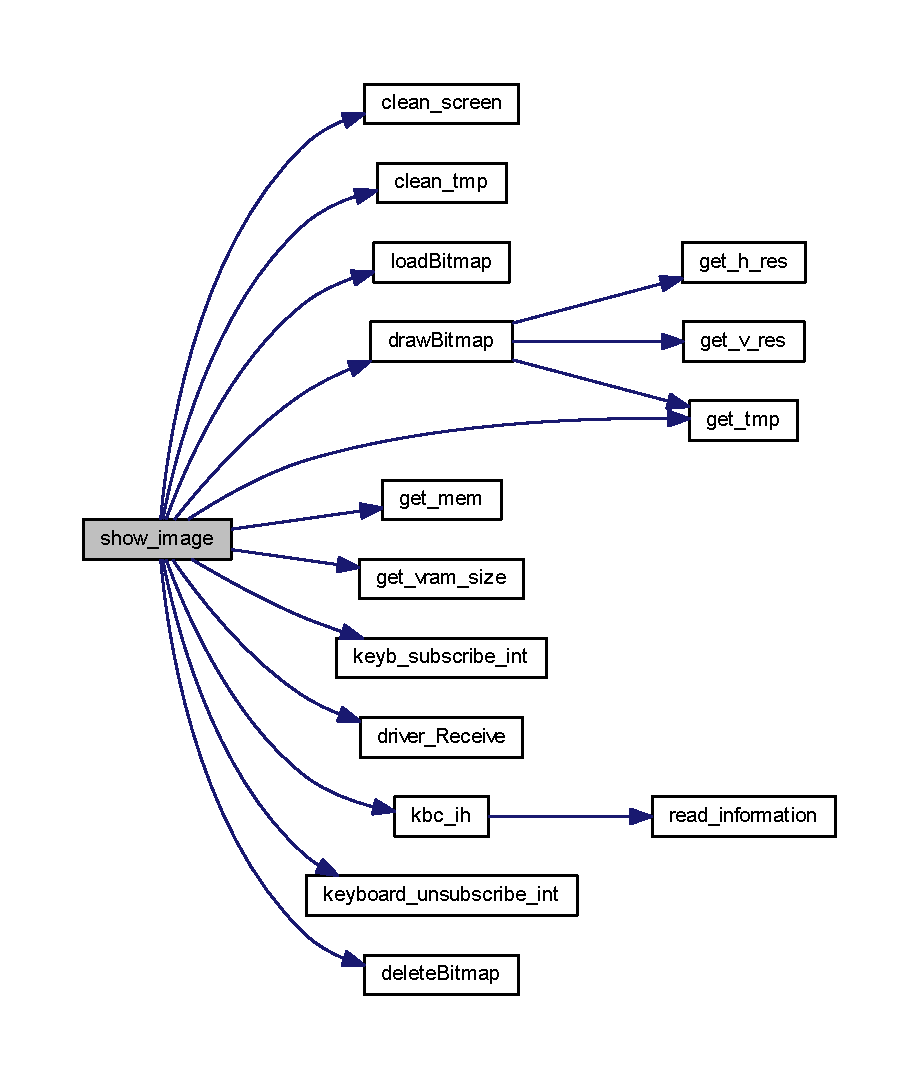
\includegraphics[width=350pt]{group__credits_ga2d90e43cf8b9ee19d3dca31eb1c9cddd_cgraph}
\end{center}
\end{figure}
Here is the caller graph for this function\+:
\nopagebreak
\begin{figure}[H]
\begin{center}
\leavevmode
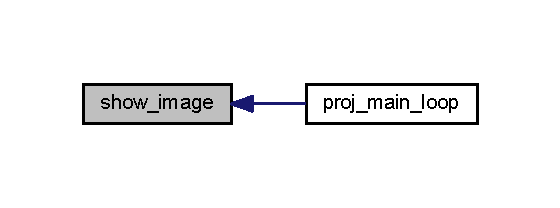
\includegraphics[width=269pt]{group__credits_ga2d90e43cf8b9ee19d3dca31eb1c9cddd_icgraph}
\end{center}
\end{figure}


\subsection{Variable Documentation}
\mbox{\Hypertarget{group__credits_ga801bef0ab9d72c95bc5d6d6a0d8f2db0}\label{group__credits_ga801bef0ab9d72c95bc5d6d6a0d8f2db0}} 
\index{credits@{credits}!image@{image}}
\index{image@{image}!credits@{credits}}
\subsubsection{\texorpdfstring{image}{image}}
{\footnotesize\ttfamily \mbox{\hyperlink{struct_bitmap}{Bitmap}}$\ast$ image}


\hypertarget{group__game}{}\section{game}
\label{group__game}\index{game@{game}}
\subsection*{Data Structures}
\begin{DoxyCompactItemize}
\item 
struct \mbox{\hyperlink{structgame_over}{game\+Over}}
\item 
struct \mbox{\hyperlink{structtetris}{tetris}}
\item 
struct \mbox{\hyperlink{structpnt}{pnt}}
\item 
struct \mbox{\hyperlink{structscoreimg}{scoreimg}}
\item 
struct \mbox{\hyperlink{structlvl}{lvl}}
\item 
struct \mbox{\hyperlink{structldig}{ldig}}
\item 
struct \mbox{\hyperlink{struct_date__image}{Date\+\_\+image}}
\end{DoxyCompactItemize}
\subsection*{Macros}
\begin{DoxyCompactItemize}
\item 
\#define \mbox{\hyperlink{group__game_ga690efe7a045abbfc9b27e560a2ec9513}{A\+M\+A\+KE}}~0x1E
\item 
\#define \mbox{\hyperlink{group__game_ga44e36af0ac2ecc5ef350ba0be8942ec2}{D\+M\+A\+KE}}~0x20
\item 
\#define \mbox{\hyperlink{group__game_gac1a92d19df172666cb200a4af8dda91c}{S\+P\+A\+C\+E\+M\+A\+KE}}~0x39
\item 
\#define \mbox{\hyperlink{group__game_ga03947a021c40104691ad783d365f4e10}{S\+M\+A\+KE}}~0x1F
\item 
\#define \mbox{\hyperlink{group__game_ga1e09a1aa8665e3937510ff8c14fc7fa7}{A\+B\+R\+E\+AK}}~0x9E
\item 
\#define \mbox{\hyperlink{group__game_gab38702ad72d18f40a1ee070106d30718}{D\+B\+R\+E\+AK}}~0x\+A0
\item 
\#define \mbox{\hyperlink{group__game_gae1b188c4c1653daaa218b7de29a1d743}{S\+P\+A\+C\+E\+B\+R\+E\+AK}}~0x\+B9
\item 
\#define \mbox{\hyperlink{group__game_ga5b832c74ca8bf6ffabf7d4190eded9f9}{S\+B\+R\+E\+AK}}~0x9F
\item 
\#define \mbox{\hyperlink{group__game_ga4af1b6159e447ba72652bb7fcdfa726e}{E\+SC}}~0x81
\item 
\#define \mbox{\hyperlink{group__game_ga8c3a1040415b05ec42d4ff34b27a7c29}{G\+A\+M\+E\+O\+V\+E\+R\+\_\+\+E\+ND}}~3
\item 
\#define \mbox{\hyperlink{group__game_ga3b5dc51b11999829eff0e40d21279e3b}{P\+O\+I\+N\+T\+S\+\_\+\+P\+E\+R\+\_\+\+L\+I\+NE}}~10
\item 
\#define \mbox{\hyperlink{group__game_ga66dedf1c8c1aefa0530444a033186ac8}{P\+O\+I\+N\+T\+S\+\_\+\+P\+E\+R\+\_\+\+L\+I\+N\+E\+\_\+2}}~30
\item 
\#define \mbox{\hyperlink{group__game_ga9de0f4d507922c46865095e4d4ddd538}{P\+O\+I\+N\+T\+S\+\_\+\+P\+E\+R\+\_\+\+L\+I\+N\+E\+\_\+3}}~40
\item 
\#define \mbox{\hyperlink{group__game_ga16a7908b8d52a1c554db7f11af689c78}{P\+O\+I\+N\+T\+S\+\_\+\+P\+E\+R\+\_\+\+L\+I\+N\+E\+\_\+4}}~60
\item 
\#define \mbox{\hyperlink{group__game_ga77fed468d8077df04b2a583249ea9ec3}{R\+A\+T\+E\+\_\+\+L\+V\+L1}}~20
\item 
\#define \mbox{\hyperlink{group__game_ga53f5b2e837f82146bdbbfcbe864a3787}{R\+A\+T\+E\+\_\+\+L\+V\+L2}}~15
\item 
\#define \mbox{\hyperlink{group__game_gad8d89481d86fee32a968b72da932456d}{R\+A\+T\+E\+\_\+\+L\+V\+L13}}~10
\item 
\#define \mbox{\hyperlink{group__game_ga43ac83d9bacb381715d00f2d81869c81}{S\+C\+O\+R\+E\+\_\+\+Y\+\_\+\+P\+OS}}~100
\item 
\#define \mbox{\hyperlink{group__game_ga52fa9d2055cff71b5a6fbdaef721dad0}{S\+C\+O\+R\+E\+\_\+\+X\+\_\+\+P\+OS}}~700
\item 
\#define \mbox{\hyperlink{group__game_ga1943a6fd02085a111e2e228b6c8257c8}{S\+C\+O\+R\+E\+\_\+\+F\+I\+N\+A\+L\+\_\+\+Y\+\_\+\+P\+OS}}~510
\item 
\#define \mbox{\hyperlink{group__game_ga0798d3f568ec40fefb913cf04738fe38}{S\+C\+O\+R\+E\+\_\+\+F\+I\+N\+A\+L\+\_\+\+X\+\_\+\+P\+OS}}~400
\item 
\#define \mbox{\hyperlink{group__game_ga3d9c227aaa4ac1d98dfb5f13af4106f2}{T\+E\+T\+R\+I\+S\+\_\+\+I\+M\+G\+\_\+X}}~400
\item 
\#define \mbox{\hyperlink{group__game_ga443a6b6a37a38501a81ab30095410ac1}{x\+\_\+b\+\_\+left}}~230
\item 
\#define \mbox{\hyperlink{group__game_gaf01c6e35b7b83fe4f9365249f997e26c}{x\+\_\+b\+\_\+right}}~550
\end{DoxyCompactItemize}
\subsection*{Functions}
\begin{DoxyCompactItemize}
\item 
void \mbox{\hyperlink{group__game_gaf426df873300d051272115729c8fa5a1}{write\+\_\+lvL}} (int level, \mbox{\hyperlink{structldig}{ldig}} $\ast$l)
\begin{DoxyCompactList}\small\item\em Writes the level on the screen. \end{DoxyCompactList}\item 
void \mbox{\hyperlink{group__game_ga4447b1a565fed3c6130bf9e38970b933}{write\+\_\+score}} (int pont, \mbox{\hyperlink{structpnt}{pnt}} $\ast$u, int x, int y)
\begin{DoxyCompactList}\small\item\em Writes the score on the screen and in the game end. \end{DoxyCompactList}\item 
void \mbox{\hyperlink{group__game_ga75e50926d07db9cfd2bad44c163f2bdd}{draw\+\_\+date\+\_\+str}} (\mbox{\hyperlink{struct_date}{Date}} \mbox{\hyperlink{game_8c_a85641069b0d4478ab8a7356c3bf32ea3}{d}}, \mbox{\hyperlink{struct_date__image}{Date\+\_\+image}} $\ast$di)
\begin{DoxyCompactList}\small\item\em Writes the date on the screen. \end{DoxyCompactList}\item 
void \mbox{\hyperlink{group__game_ga11d44633d3eb30282274511c8a8d7511}{paint\+\_\+game}} ()
\begin{DoxyCompactList}\small\item\em Draws on the screen the exteriors of the game\+: title, borders,score and level. \end{DoxyCompactList}\item 
void \mbox{\hyperlink{group__game_ga553ba6d099151083884ae0d6c1e76771}{game\+\_\+movement\+\_\+options}} (uint32\+\_\+t \mbox{\hyperlink{mouse_8c_a325819a8e492ac69542e8b31705af6e9}{data}}, int $\ast$make\+\_\+nbr, \mbox{\hyperlink{struct_tetramino}{Tetramino}} $\ast$t)
\begin{DoxyCompactList}\small\item\em Receives keyboard information and handles the event of the game accordingly. \end{DoxyCompactList}\item 
int \mbox{\hyperlink{group__game_gaa449f1959d3595ac0d0b88d643b1acd4}{game\+\_\+main}} ()
\begin{DoxyCompactList}\small\item\em Main function of the game, handles the flow of the game and presents the info to the player. \end{DoxyCompactList}\item 
void \mbox{\hyperlink{group__game_gac6c44260c9d002d8a21c4bfd44b2fd88}{delete\+\_\+info}} (\mbox{\hyperlink{structpnt}{pnt}} $\ast$u, \mbox{\hyperlink{structldig}{ldig}} $\ast$ld, \mbox{\hyperlink{struct_date__image}{Date\+\_\+image}} $\ast$dimag)
\begin{DoxyCompactList}\small\item\em Deletes the allocated memory, allowing to free memory space. \end{DoxyCompactList}\item 
uint8\+\_\+t \mbox{\hyperlink{group__game_ga221b757ab658deb87f4ccd865d29a9ff}{driver\+\_\+\+Receive}} (endpoint\+\_\+t any, message $\ast$m, int $\ast$\mbox{\hyperlink{game_8c_ab9f863ebaa3805a6e366e055cd35626a}{ipc\+\_\+status}})
\begin{DoxyCompactList}\small\item\em Wrapper function for driver\+\_\+receive. Used only for function call graph. \end{DoxyCompactList}\end{DoxyCompactItemize}
\subsection*{Variables}
\begin{DoxyCompactItemize}
\item 
\mbox{\hyperlink{struct_bitmap}{Bitmap}} $\ast$ \mbox{\hyperlink{group__game_ga801bef0ab9d72c95bc5d6d6a0d8f2db0}{image}}
\item 
\mbox{\hyperlink{struct_bitmap}{Bitmap}} $\ast$ \mbox{\hyperlink{group__game_ga801bef0ab9d72c95bc5d6d6a0d8f2db0}{image}}
\item 
\mbox{\hyperlink{struct_bitmap}{Bitmap}} $\ast$ \mbox{\hyperlink{group__game_ga801bef0ab9d72c95bc5d6d6a0d8f2db0}{image}}
\item 
\mbox{\hyperlink{struct_bitmap}{Bitmap}} $\ast$ \mbox{\hyperlink{group__game_ga801bef0ab9d72c95bc5d6d6a0d8f2db0}{image}}
\item 
\mbox{\hyperlink{struct_bitmap}{Bitmap}} $\ast$ \mbox{\hyperlink{group__game_ga801bef0ab9d72c95bc5d6d6a0d8f2db0}{image}}
\item 
\mbox{\hyperlink{struct_bitmap}{Bitmap}} $\ast$ \mbox{\hyperlink{group__game_ga801bef0ab9d72c95bc5d6d6a0d8f2db0}{image}}
\item 
\mbox{\hyperlink{struct_bitmap}{Bitmap}} $\ast$ \mbox{\hyperlink{group__game_ga801bef0ab9d72c95bc5d6d6a0d8f2db0}{image}}
\end{DoxyCompactItemize}


\subsection{Detailed Description}
Functions for handling the game 

\subsection{Macro Definition Documentation}
\mbox{\Hypertarget{group__game_ga1e09a1aa8665e3937510ff8c14fc7fa7}\label{group__game_ga1e09a1aa8665e3937510ff8c14fc7fa7}} 
\index{game@{game}!A\+B\+R\+E\+AK@{A\+B\+R\+E\+AK}}
\index{A\+B\+R\+E\+AK@{A\+B\+R\+E\+AK}!game@{game}}
\subsubsection{\texorpdfstring{A\+B\+R\+E\+AK}{ABREAK}}
{\footnotesize\ttfamily \#define A\+B\+R\+E\+AK~0x9E}

\mbox{\Hypertarget{group__game_ga690efe7a045abbfc9b27e560a2ec9513}\label{group__game_ga690efe7a045abbfc9b27e560a2ec9513}} 
\index{game@{game}!A\+M\+A\+KE@{A\+M\+A\+KE}}
\index{A\+M\+A\+KE@{A\+M\+A\+KE}!game@{game}}
\subsubsection{\texorpdfstring{A\+M\+A\+KE}{AMAKE}}
{\footnotesize\ttfamily \#define A\+M\+A\+KE~0x1E}

\mbox{\Hypertarget{group__game_gab38702ad72d18f40a1ee070106d30718}\label{group__game_gab38702ad72d18f40a1ee070106d30718}} 
\index{game@{game}!D\+B\+R\+E\+AK@{D\+B\+R\+E\+AK}}
\index{D\+B\+R\+E\+AK@{D\+B\+R\+E\+AK}!game@{game}}
\subsubsection{\texorpdfstring{D\+B\+R\+E\+AK}{DBREAK}}
{\footnotesize\ttfamily \#define D\+B\+R\+E\+AK~0x\+A0}

\mbox{\Hypertarget{group__game_ga44e36af0ac2ecc5ef350ba0be8942ec2}\label{group__game_ga44e36af0ac2ecc5ef350ba0be8942ec2}} 
\index{game@{game}!D\+M\+A\+KE@{D\+M\+A\+KE}}
\index{D\+M\+A\+KE@{D\+M\+A\+KE}!game@{game}}
\subsubsection{\texorpdfstring{D\+M\+A\+KE}{DMAKE}}
{\footnotesize\ttfamily \#define D\+M\+A\+KE~0x20}

\mbox{\Hypertarget{group__game_ga4af1b6159e447ba72652bb7fcdfa726e}\label{group__game_ga4af1b6159e447ba72652bb7fcdfa726e}} 
\index{game@{game}!E\+SC@{E\+SC}}
\index{E\+SC@{E\+SC}!game@{game}}
\subsubsection{\texorpdfstring{E\+SC}{ESC}}
{\footnotesize\ttfamily \#define E\+SC~0x81}

\mbox{\Hypertarget{group__game_ga8c3a1040415b05ec42d4ff34b27a7c29}\label{group__game_ga8c3a1040415b05ec42d4ff34b27a7c29}} 
\index{game@{game}!G\+A\+M\+E\+O\+V\+E\+R\+\_\+\+E\+ND@{G\+A\+M\+E\+O\+V\+E\+R\+\_\+\+E\+ND}}
\index{G\+A\+M\+E\+O\+V\+E\+R\+\_\+\+E\+ND@{G\+A\+M\+E\+O\+V\+E\+R\+\_\+\+E\+ND}!game@{game}}
\subsubsection{\texorpdfstring{G\+A\+M\+E\+O\+V\+E\+R\+\_\+\+E\+ND}{GAMEOVER\_END}}
{\footnotesize\ttfamily \#define G\+A\+M\+E\+O\+V\+E\+R\+\_\+\+E\+ND~3}

\mbox{\Hypertarget{group__game_ga3b5dc51b11999829eff0e40d21279e3b}\label{group__game_ga3b5dc51b11999829eff0e40d21279e3b}} 
\index{game@{game}!P\+O\+I\+N\+T\+S\+\_\+\+P\+E\+R\+\_\+\+L\+I\+NE@{P\+O\+I\+N\+T\+S\+\_\+\+P\+E\+R\+\_\+\+L\+I\+NE}}
\index{P\+O\+I\+N\+T\+S\+\_\+\+P\+E\+R\+\_\+\+L\+I\+NE@{P\+O\+I\+N\+T\+S\+\_\+\+P\+E\+R\+\_\+\+L\+I\+NE}!game@{game}}
\subsubsection{\texorpdfstring{P\+O\+I\+N\+T\+S\+\_\+\+P\+E\+R\+\_\+\+L\+I\+NE}{POINTS\_PER\_LINE}}
{\footnotesize\ttfamily \#define P\+O\+I\+N\+T\+S\+\_\+\+P\+E\+R\+\_\+\+L\+I\+NE~10}

\mbox{\Hypertarget{group__game_ga66dedf1c8c1aefa0530444a033186ac8}\label{group__game_ga66dedf1c8c1aefa0530444a033186ac8}} 
\index{game@{game}!P\+O\+I\+N\+T\+S\+\_\+\+P\+E\+R\+\_\+\+L\+I\+N\+E\+\_\+2@{P\+O\+I\+N\+T\+S\+\_\+\+P\+E\+R\+\_\+\+L\+I\+N\+E\+\_\+2}}
\index{P\+O\+I\+N\+T\+S\+\_\+\+P\+E\+R\+\_\+\+L\+I\+N\+E\+\_\+2@{P\+O\+I\+N\+T\+S\+\_\+\+P\+E\+R\+\_\+\+L\+I\+N\+E\+\_\+2}!game@{game}}
\subsubsection{\texorpdfstring{P\+O\+I\+N\+T\+S\+\_\+\+P\+E\+R\+\_\+\+L\+I\+N\+E\+\_\+2}{POINTS\_PER\_LINE\_2}}
{\footnotesize\ttfamily \#define P\+O\+I\+N\+T\+S\+\_\+\+P\+E\+R\+\_\+\+L\+I\+N\+E\+\_\+2~30}

\mbox{\Hypertarget{group__game_ga9de0f4d507922c46865095e4d4ddd538}\label{group__game_ga9de0f4d507922c46865095e4d4ddd538}} 
\index{game@{game}!P\+O\+I\+N\+T\+S\+\_\+\+P\+E\+R\+\_\+\+L\+I\+N\+E\+\_\+3@{P\+O\+I\+N\+T\+S\+\_\+\+P\+E\+R\+\_\+\+L\+I\+N\+E\+\_\+3}}
\index{P\+O\+I\+N\+T\+S\+\_\+\+P\+E\+R\+\_\+\+L\+I\+N\+E\+\_\+3@{P\+O\+I\+N\+T\+S\+\_\+\+P\+E\+R\+\_\+\+L\+I\+N\+E\+\_\+3}!game@{game}}
\subsubsection{\texorpdfstring{P\+O\+I\+N\+T\+S\+\_\+\+P\+E\+R\+\_\+\+L\+I\+N\+E\+\_\+3}{POINTS\_PER\_LINE\_3}}
{\footnotesize\ttfamily \#define P\+O\+I\+N\+T\+S\+\_\+\+P\+E\+R\+\_\+\+L\+I\+N\+E\+\_\+3~40}

\mbox{\Hypertarget{group__game_ga16a7908b8d52a1c554db7f11af689c78}\label{group__game_ga16a7908b8d52a1c554db7f11af689c78}} 
\index{game@{game}!P\+O\+I\+N\+T\+S\+\_\+\+P\+E\+R\+\_\+\+L\+I\+N\+E\+\_\+4@{P\+O\+I\+N\+T\+S\+\_\+\+P\+E\+R\+\_\+\+L\+I\+N\+E\+\_\+4}}
\index{P\+O\+I\+N\+T\+S\+\_\+\+P\+E\+R\+\_\+\+L\+I\+N\+E\+\_\+4@{P\+O\+I\+N\+T\+S\+\_\+\+P\+E\+R\+\_\+\+L\+I\+N\+E\+\_\+4}!game@{game}}
\subsubsection{\texorpdfstring{P\+O\+I\+N\+T\+S\+\_\+\+P\+E\+R\+\_\+\+L\+I\+N\+E\+\_\+4}{POINTS\_PER\_LINE\_4}}
{\footnotesize\ttfamily \#define P\+O\+I\+N\+T\+S\+\_\+\+P\+E\+R\+\_\+\+L\+I\+N\+E\+\_\+4~60}

\mbox{\Hypertarget{group__game_ga77fed468d8077df04b2a583249ea9ec3}\label{group__game_ga77fed468d8077df04b2a583249ea9ec3}} 
\index{game@{game}!R\+A\+T\+E\+\_\+\+L\+V\+L1@{R\+A\+T\+E\+\_\+\+L\+V\+L1}}
\index{R\+A\+T\+E\+\_\+\+L\+V\+L1@{R\+A\+T\+E\+\_\+\+L\+V\+L1}!game@{game}}
\subsubsection{\texorpdfstring{R\+A\+T\+E\+\_\+\+L\+V\+L1}{RATE\_LVL1}}
{\footnotesize\ttfamily \#define R\+A\+T\+E\+\_\+\+L\+V\+L1~20}

\mbox{\Hypertarget{group__game_gad8d89481d86fee32a968b72da932456d}\label{group__game_gad8d89481d86fee32a968b72da932456d}} 
\index{game@{game}!R\+A\+T\+E\+\_\+\+L\+V\+L13@{R\+A\+T\+E\+\_\+\+L\+V\+L13}}
\index{R\+A\+T\+E\+\_\+\+L\+V\+L13@{R\+A\+T\+E\+\_\+\+L\+V\+L13}!game@{game}}
\subsubsection{\texorpdfstring{R\+A\+T\+E\+\_\+\+L\+V\+L13}{RATE\_LVL13}}
{\footnotesize\ttfamily \#define R\+A\+T\+E\+\_\+\+L\+V\+L13~10}

\mbox{\Hypertarget{group__game_ga53f5b2e837f82146bdbbfcbe864a3787}\label{group__game_ga53f5b2e837f82146bdbbfcbe864a3787}} 
\index{game@{game}!R\+A\+T\+E\+\_\+\+L\+V\+L2@{R\+A\+T\+E\+\_\+\+L\+V\+L2}}
\index{R\+A\+T\+E\+\_\+\+L\+V\+L2@{R\+A\+T\+E\+\_\+\+L\+V\+L2}!game@{game}}
\subsubsection{\texorpdfstring{R\+A\+T\+E\+\_\+\+L\+V\+L2}{RATE\_LVL2}}
{\footnotesize\ttfamily \#define R\+A\+T\+E\+\_\+\+L\+V\+L2~15}

\mbox{\Hypertarget{group__game_ga5b832c74ca8bf6ffabf7d4190eded9f9}\label{group__game_ga5b832c74ca8bf6ffabf7d4190eded9f9}} 
\index{game@{game}!S\+B\+R\+E\+AK@{S\+B\+R\+E\+AK}}
\index{S\+B\+R\+E\+AK@{S\+B\+R\+E\+AK}!game@{game}}
\subsubsection{\texorpdfstring{S\+B\+R\+E\+AK}{SBREAK}}
{\footnotesize\ttfamily \#define S\+B\+R\+E\+AK~0x9F}

\mbox{\Hypertarget{group__game_ga0798d3f568ec40fefb913cf04738fe38}\label{group__game_ga0798d3f568ec40fefb913cf04738fe38}} 
\index{game@{game}!S\+C\+O\+R\+E\+\_\+\+F\+I\+N\+A\+L\+\_\+\+X\+\_\+\+P\+OS@{S\+C\+O\+R\+E\+\_\+\+F\+I\+N\+A\+L\+\_\+\+X\+\_\+\+P\+OS}}
\index{S\+C\+O\+R\+E\+\_\+\+F\+I\+N\+A\+L\+\_\+\+X\+\_\+\+P\+OS@{S\+C\+O\+R\+E\+\_\+\+F\+I\+N\+A\+L\+\_\+\+X\+\_\+\+P\+OS}!game@{game}}
\subsubsection{\texorpdfstring{S\+C\+O\+R\+E\+\_\+\+F\+I\+N\+A\+L\+\_\+\+X\+\_\+\+P\+OS}{SCORE\_FINAL\_X\_POS}}
{\footnotesize\ttfamily \#define S\+C\+O\+R\+E\+\_\+\+F\+I\+N\+A\+L\+\_\+\+X\+\_\+\+P\+OS~400}

\mbox{\Hypertarget{group__game_ga1943a6fd02085a111e2e228b6c8257c8}\label{group__game_ga1943a6fd02085a111e2e228b6c8257c8}} 
\index{game@{game}!S\+C\+O\+R\+E\+\_\+\+F\+I\+N\+A\+L\+\_\+\+Y\+\_\+\+P\+OS@{S\+C\+O\+R\+E\+\_\+\+F\+I\+N\+A\+L\+\_\+\+Y\+\_\+\+P\+OS}}
\index{S\+C\+O\+R\+E\+\_\+\+F\+I\+N\+A\+L\+\_\+\+Y\+\_\+\+P\+OS@{S\+C\+O\+R\+E\+\_\+\+F\+I\+N\+A\+L\+\_\+\+Y\+\_\+\+P\+OS}!game@{game}}
\subsubsection{\texorpdfstring{S\+C\+O\+R\+E\+\_\+\+F\+I\+N\+A\+L\+\_\+\+Y\+\_\+\+P\+OS}{SCORE\_FINAL\_Y\_POS}}
{\footnotesize\ttfamily \#define S\+C\+O\+R\+E\+\_\+\+F\+I\+N\+A\+L\+\_\+\+Y\+\_\+\+P\+OS~510}

\mbox{\Hypertarget{group__game_ga52fa9d2055cff71b5a6fbdaef721dad0}\label{group__game_ga52fa9d2055cff71b5a6fbdaef721dad0}} 
\index{game@{game}!S\+C\+O\+R\+E\+\_\+\+X\+\_\+\+P\+OS@{S\+C\+O\+R\+E\+\_\+\+X\+\_\+\+P\+OS}}
\index{S\+C\+O\+R\+E\+\_\+\+X\+\_\+\+P\+OS@{S\+C\+O\+R\+E\+\_\+\+X\+\_\+\+P\+OS}!game@{game}}
\subsubsection{\texorpdfstring{S\+C\+O\+R\+E\+\_\+\+X\+\_\+\+P\+OS}{SCORE\_X\_POS}}
{\footnotesize\ttfamily \#define S\+C\+O\+R\+E\+\_\+\+X\+\_\+\+P\+OS~700}

\mbox{\Hypertarget{group__game_ga43ac83d9bacb381715d00f2d81869c81}\label{group__game_ga43ac83d9bacb381715d00f2d81869c81}} 
\index{game@{game}!S\+C\+O\+R\+E\+\_\+\+Y\+\_\+\+P\+OS@{S\+C\+O\+R\+E\+\_\+\+Y\+\_\+\+P\+OS}}
\index{S\+C\+O\+R\+E\+\_\+\+Y\+\_\+\+P\+OS@{S\+C\+O\+R\+E\+\_\+\+Y\+\_\+\+P\+OS}!game@{game}}
\subsubsection{\texorpdfstring{S\+C\+O\+R\+E\+\_\+\+Y\+\_\+\+P\+OS}{SCORE\_Y\_POS}}
{\footnotesize\ttfamily \#define S\+C\+O\+R\+E\+\_\+\+Y\+\_\+\+P\+OS~100}

\mbox{\Hypertarget{group__game_ga03947a021c40104691ad783d365f4e10}\label{group__game_ga03947a021c40104691ad783d365f4e10}} 
\index{game@{game}!S\+M\+A\+KE@{S\+M\+A\+KE}}
\index{S\+M\+A\+KE@{S\+M\+A\+KE}!game@{game}}
\subsubsection{\texorpdfstring{S\+M\+A\+KE}{SMAKE}}
{\footnotesize\ttfamily \#define S\+M\+A\+KE~0x1F}

\mbox{\Hypertarget{group__game_gae1b188c4c1653daaa218b7de29a1d743}\label{group__game_gae1b188c4c1653daaa218b7de29a1d743}} 
\index{game@{game}!S\+P\+A\+C\+E\+B\+R\+E\+AK@{S\+P\+A\+C\+E\+B\+R\+E\+AK}}
\index{S\+P\+A\+C\+E\+B\+R\+E\+AK@{S\+P\+A\+C\+E\+B\+R\+E\+AK}!game@{game}}
\subsubsection{\texorpdfstring{S\+P\+A\+C\+E\+B\+R\+E\+AK}{SPACEBREAK}}
{\footnotesize\ttfamily \#define S\+P\+A\+C\+E\+B\+R\+E\+AK~0x\+B9}

\mbox{\Hypertarget{group__game_gac1a92d19df172666cb200a4af8dda91c}\label{group__game_gac1a92d19df172666cb200a4af8dda91c}} 
\index{game@{game}!S\+P\+A\+C\+E\+M\+A\+KE@{S\+P\+A\+C\+E\+M\+A\+KE}}
\index{S\+P\+A\+C\+E\+M\+A\+KE@{S\+P\+A\+C\+E\+M\+A\+KE}!game@{game}}
\subsubsection{\texorpdfstring{S\+P\+A\+C\+E\+M\+A\+KE}{SPACEMAKE}}
{\footnotesize\ttfamily \#define S\+P\+A\+C\+E\+M\+A\+KE~0x39}

\mbox{\Hypertarget{group__game_ga3d9c227aaa4ac1d98dfb5f13af4106f2}\label{group__game_ga3d9c227aaa4ac1d98dfb5f13af4106f2}} 
\index{game@{game}!T\+E\+T\+R\+I\+S\+\_\+\+I\+M\+G\+\_\+X@{T\+E\+T\+R\+I\+S\+\_\+\+I\+M\+G\+\_\+X}}
\index{T\+E\+T\+R\+I\+S\+\_\+\+I\+M\+G\+\_\+X@{T\+E\+T\+R\+I\+S\+\_\+\+I\+M\+G\+\_\+X}!game@{game}}
\subsubsection{\texorpdfstring{T\+E\+T\+R\+I\+S\+\_\+\+I\+M\+G\+\_\+X}{TETRIS\_IMG\_X}}
{\footnotesize\ttfamily \#define T\+E\+T\+R\+I\+S\+\_\+\+I\+M\+G\+\_\+X~400}

\mbox{\Hypertarget{group__game_ga443a6b6a37a38501a81ab30095410ac1}\label{group__game_ga443a6b6a37a38501a81ab30095410ac1}} 
\index{game@{game}!x\+\_\+b\+\_\+left@{x\+\_\+b\+\_\+left}}
\index{x\+\_\+b\+\_\+left@{x\+\_\+b\+\_\+left}!game@{game}}
\subsubsection{\texorpdfstring{x\+\_\+b\+\_\+left}{x\_b\_left}}
{\footnotesize\ttfamily \#define x\+\_\+b\+\_\+left~230}

\mbox{\Hypertarget{group__game_gaf01c6e35b7b83fe4f9365249f997e26c}\label{group__game_gaf01c6e35b7b83fe4f9365249f997e26c}} 
\index{game@{game}!x\+\_\+b\+\_\+right@{x\+\_\+b\+\_\+right}}
\index{x\+\_\+b\+\_\+right@{x\+\_\+b\+\_\+right}!game@{game}}
\subsubsection{\texorpdfstring{x\+\_\+b\+\_\+right}{x\_b\_right}}
{\footnotesize\ttfamily \#define x\+\_\+b\+\_\+right~550}



\subsection{Function Documentation}
\mbox{\Hypertarget{group__game_gac6c44260c9d002d8a21c4bfd44b2fd88}\label{group__game_gac6c44260c9d002d8a21c4bfd44b2fd88}} 
\index{game@{game}!delete\+\_\+info@{delete\+\_\+info}}
\index{delete\+\_\+info@{delete\+\_\+info}!game@{game}}
\subsubsection{\texorpdfstring{delete\+\_\+info()}{delete\_info()}}
{\footnotesize\ttfamily void delete\+\_\+info (\begin{DoxyParamCaption}\item[{\mbox{\hyperlink{structpnt}{pnt}} $\ast$}]{u,  }\item[{\mbox{\hyperlink{structldig}{ldig}} $\ast$}]{ld,  }\item[{\mbox{\hyperlink{struct_date__image}{Date\+\_\+image}} $\ast$}]{dimag }\end{DoxyParamCaption})}



Deletes the allocated memory, allowing to free memory space. 


\begin{DoxyParams}{Parameters}
{\em u} & -\/ Pointer to the struct where the score bitmap is stored \\
\hline
{\em ld} & -\/ Pointer to the struct where the level bitmap is stored \\
\hline
{\em dimag} & -\/ Pointer to the struct where the date bitmap is stored \\
\hline
\end{DoxyParams}
Here is the caller graph for this function\+:
\nopagebreak
\begin{figure}[H]
\begin{center}
\leavevmode
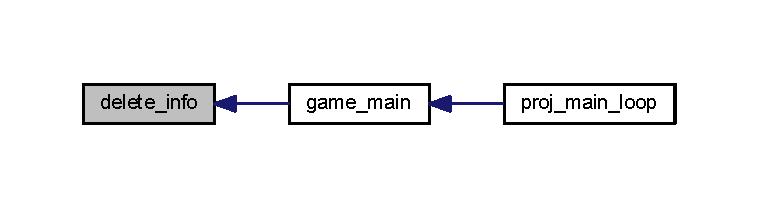
\includegraphics[width=350pt]{group__game_gac6c44260c9d002d8a21c4bfd44b2fd88_icgraph}
\end{center}
\end{figure}
\mbox{\Hypertarget{group__game_ga75e50926d07db9cfd2bad44c163f2bdd}\label{group__game_ga75e50926d07db9cfd2bad44c163f2bdd}} 
\index{game@{game}!draw\+\_\+date\+\_\+str@{draw\+\_\+date\+\_\+str}}
\index{draw\+\_\+date\+\_\+str@{draw\+\_\+date\+\_\+str}!game@{game}}
\subsubsection{\texorpdfstring{draw\+\_\+date\+\_\+str()}{draw\_date\_str()}}
{\footnotesize\ttfamily void draw\+\_\+date\+\_\+str (\begin{DoxyParamCaption}\item[{\mbox{\hyperlink{struct_date}{Date}}}]{d,  }\item[{\mbox{\hyperlink{struct_date__image}{Date\+\_\+image}} $\ast$}]{di }\end{DoxyParamCaption})}



Writes the date on the screen. 


\begin{DoxyParams}{Parameters}
{\em d} & -\/ Contains information about the date \\
\hline
{\em di} & -\/ Pointer to the struct in which is stored the bitmap of the date \\
\hline
\end{DoxyParams}
Here is the call graph for this function\+:
\nopagebreak
\begin{figure}[H]
\begin{center}
\leavevmode
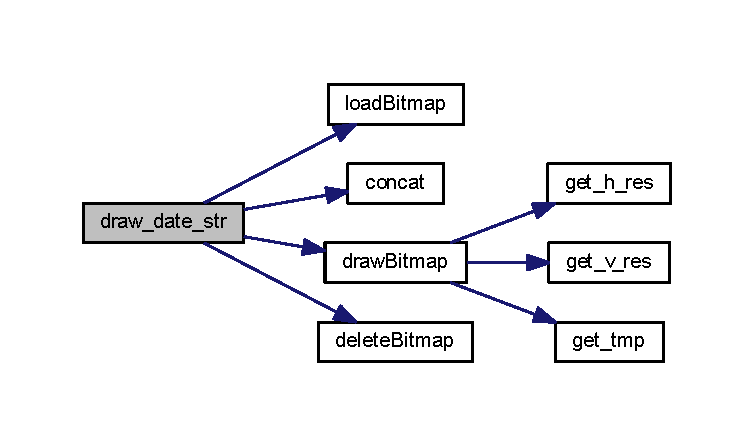
\includegraphics[width=350pt]{group__game_ga75e50926d07db9cfd2bad44c163f2bdd_cgraph}
\end{center}
\end{figure}
Here is the caller graph for this function\+:
\nopagebreak
\begin{figure}[H]
\begin{center}
\leavevmode
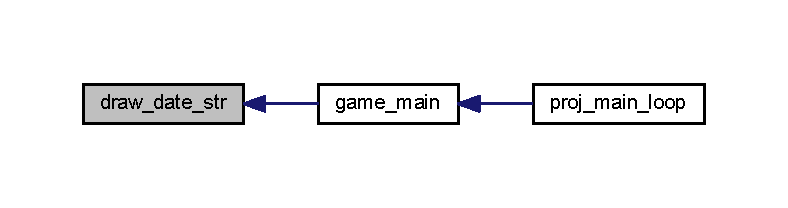
\includegraphics[width=350pt]{group__game_ga75e50926d07db9cfd2bad44c163f2bdd_icgraph}
\end{center}
\end{figure}
\mbox{\Hypertarget{group__game_ga221b757ab658deb87f4ccd865d29a9ff}\label{group__game_ga221b757ab658deb87f4ccd865d29a9ff}} 
\index{game@{game}!driver\+\_\+\+Receive@{driver\+\_\+\+Receive}}
\index{driver\+\_\+\+Receive@{driver\+\_\+\+Receive}!game@{game}}
\subsubsection{\texorpdfstring{driver\+\_\+\+Receive()}{driver\_Receive()}}
{\footnotesize\ttfamily uint8\+\_\+t driver\+\_\+\+Receive (\begin{DoxyParamCaption}\item[{endpoint\+\_\+t}]{any,  }\item[{message $\ast$}]{m,  }\item[{int $\ast$}]{ipc\+\_\+status }\end{DoxyParamCaption})}



Wrapper function for driver\+\_\+receive. Used only for function call graph. 


\begin{DoxyParams}{Parameters}
{\em any} & \\
\hline
{\em m} & \\
\hline
{\em ipc\+\_\+status} & \\
\hline
\end{DoxyParams}
\begin{DoxyReturn}{Returns}
uint8\+\_\+t 
\end{DoxyReturn}
Here is the caller graph for this function\+:
\nopagebreak
\begin{figure}[H]
\begin{center}
\leavevmode
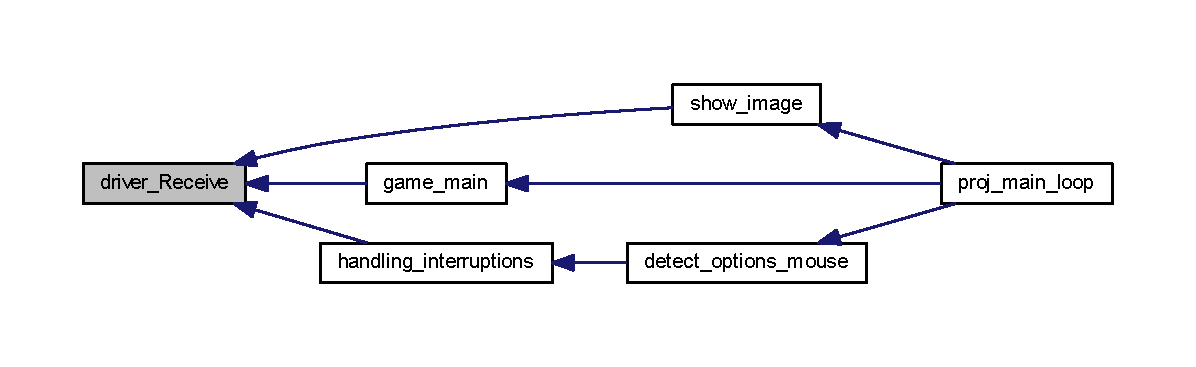
\includegraphics[width=350pt]{group__game_ga221b757ab658deb87f4ccd865d29a9ff_icgraph}
\end{center}
\end{figure}
\mbox{\Hypertarget{group__game_gaa449f1959d3595ac0d0b88d643b1acd4}\label{group__game_gaa449f1959d3595ac0d0b88d643b1acd4}} 
\index{game@{game}!game\+\_\+main@{game\+\_\+main}}
\index{game\+\_\+main@{game\+\_\+main}!game@{game}}
\subsubsection{\texorpdfstring{game\+\_\+main()}{game\_main()}}
{\footnotesize\ttfamily int game\+\_\+main (\begin{DoxyParamCaption}{ }\end{DoxyParamCaption})}



Main function of the game, handles the flow of the game and presents the info to the player. 

\begin{DoxyReturn}{Returns}
int -\/ Returns 0 if all went as expected, returns 1 otherwise 
\end{DoxyReturn}
Here is the call graph for this function\+:
\nopagebreak
\begin{figure}[H]
\begin{center}
\leavevmode
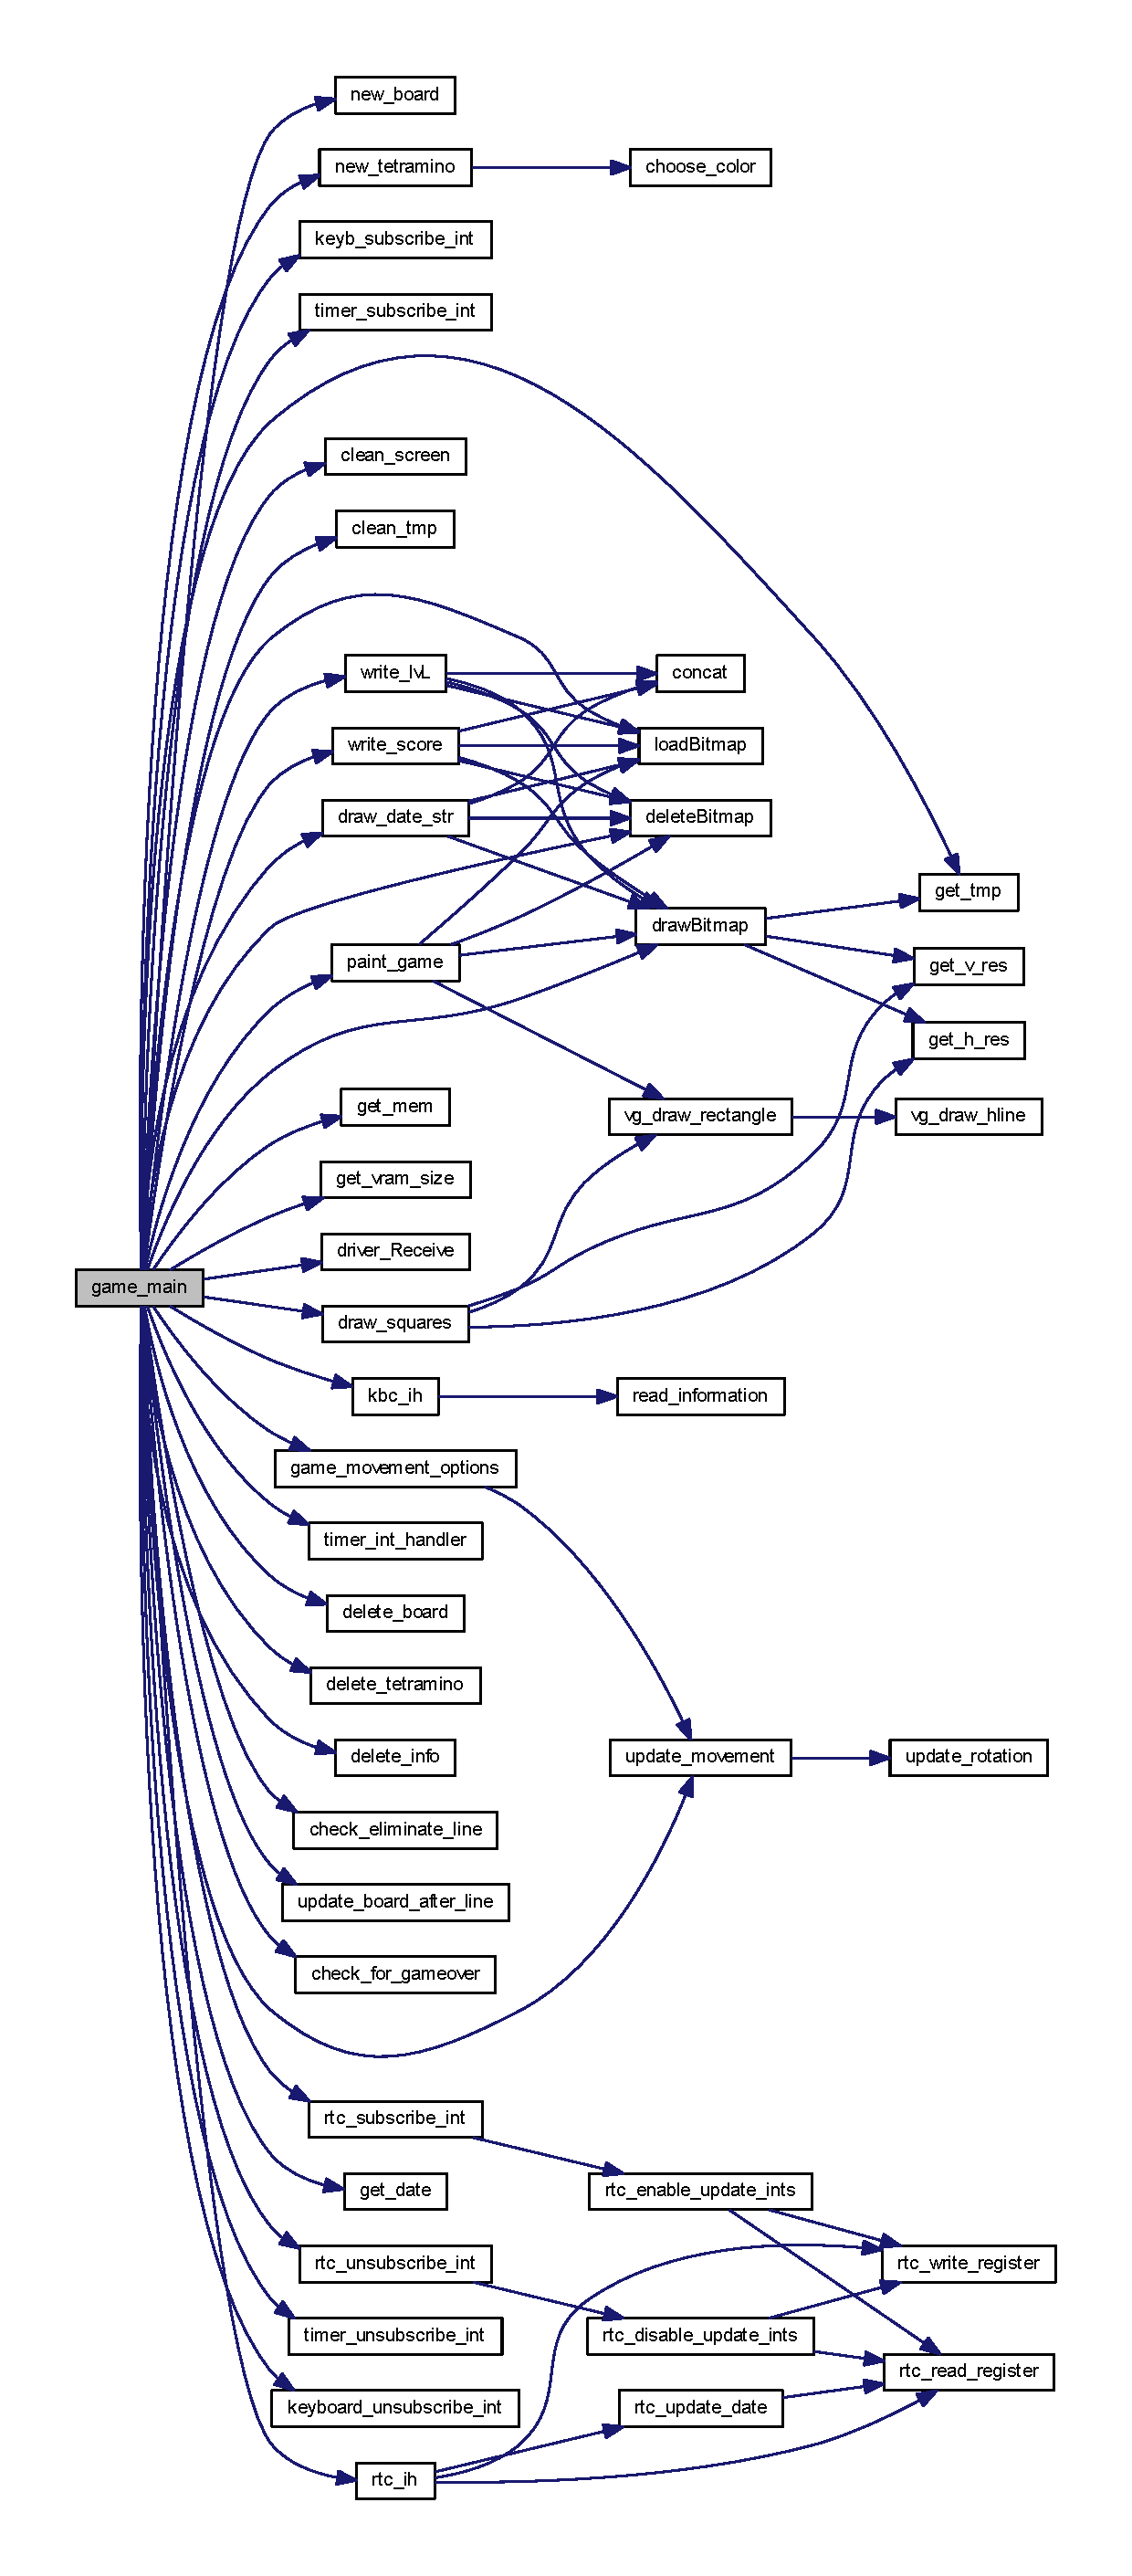
\includegraphics[height=550pt]{group__game_gaa449f1959d3595ac0d0b88d643b1acd4_cgraph}
\end{center}
\end{figure}
Here is the caller graph for this function\+:
\nopagebreak
\begin{figure}[H]
\begin{center}
\leavevmode
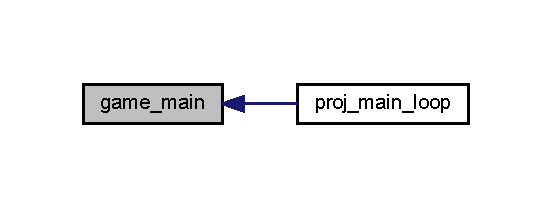
\includegraphics[width=265pt]{group__game_gaa449f1959d3595ac0d0b88d643b1acd4_icgraph}
\end{center}
\end{figure}
\mbox{\Hypertarget{group__game_ga553ba6d099151083884ae0d6c1e76771}\label{group__game_ga553ba6d099151083884ae0d6c1e76771}} 
\index{game@{game}!game\+\_\+movement\+\_\+options@{game\+\_\+movement\+\_\+options}}
\index{game\+\_\+movement\+\_\+options@{game\+\_\+movement\+\_\+options}!game@{game}}
\subsubsection{\texorpdfstring{game\+\_\+movement\+\_\+options()}{game\_movement\_options()}}
{\footnotesize\ttfamily void game\+\_\+movement\+\_\+options (\begin{DoxyParamCaption}\item[{uint32\+\_\+t}]{data,  }\item[{int $\ast$}]{make\+\_\+nbr,  }\item[{\mbox{\hyperlink{struct_tetramino}{Tetramino}} $\ast$}]{t }\end{DoxyParamCaption})}



Receives keyboard information and handles the event of the game accordingly. 


\begin{DoxyParams}{Parameters}
{\em data} & -\/ keyboard scancode \\
\hline
{\em make\+\_\+nbr} & -\/ keeps track of the times a key is pressed to prevent unexpected movements \\
\hline
{\em t} & -\/ Pointer to the struct that contains the information about a tetramino \\
\hline
\end{DoxyParams}
Here is the call graph for this function\+:
\nopagebreak
\begin{figure}[H]
\begin{center}
\leavevmode
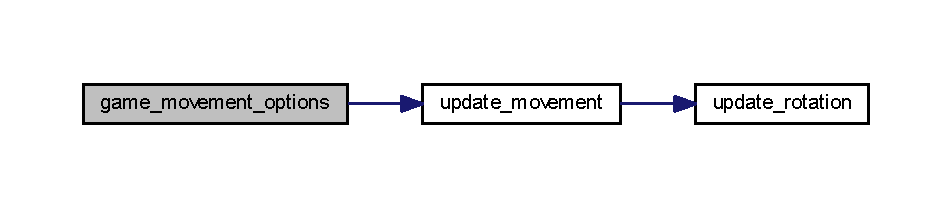
\includegraphics[width=350pt]{group__game_ga553ba6d099151083884ae0d6c1e76771_cgraph}
\end{center}
\end{figure}
Here is the caller graph for this function\+:
\nopagebreak
\begin{figure}[H]
\begin{center}
\leavevmode
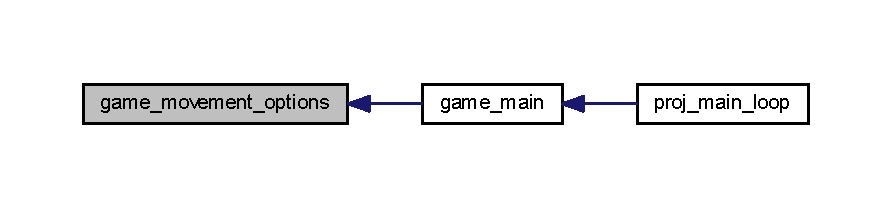
\includegraphics[width=350pt]{group__game_ga553ba6d099151083884ae0d6c1e76771_icgraph}
\end{center}
\end{figure}
\mbox{\Hypertarget{group__game_ga11d44633d3eb30282274511c8a8d7511}\label{group__game_ga11d44633d3eb30282274511c8a8d7511}} 
\index{game@{game}!paint\+\_\+game@{paint\+\_\+game}}
\index{paint\+\_\+game@{paint\+\_\+game}!game@{game}}
\subsubsection{\texorpdfstring{paint\+\_\+game()}{paint\_game()}}
{\footnotesize\ttfamily void paint\+\_\+game (\begin{DoxyParamCaption}{ }\end{DoxyParamCaption})}



Draws on the screen the exteriors of the game\+: title, borders,score and level. 

Here is the call graph for this function\+:
\nopagebreak
\begin{figure}[H]
\begin{center}
\leavevmode
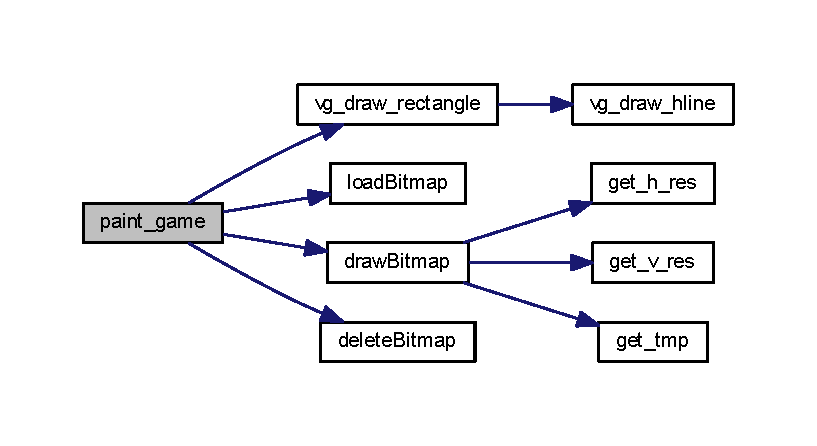
\includegraphics[width=350pt]{group__game_ga11d44633d3eb30282274511c8a8d7511_cgraph}
\end{center}
\end{figure}
Here is the caller graph for this function\+:
\nopagebreak
\begin{figure}[H]
\begin{center}
\leavevmode
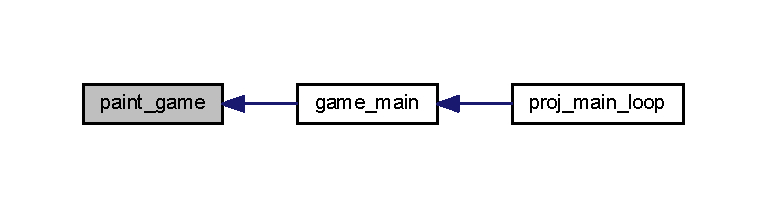
\includegraphics[width=350pt]{group__game_ga11d44633d3eb30282274511c8a8d7511_icgraph}
\end{center}
\end{figure}
\mbox{\Hypertarget{group__game_gaf426df873300d051272115729c8fa5a1}\label{group__game_gaf426df873300d051272115729c8fa5a1}} 
\index{game@{game}!write\+\_\+lvL@{write\+\_\+lvL}}
\index{write\+\_\+lvL@{write\+\_\+lvL}!game@{game}}
\subsubsection{\texorpdfstring{write\+\_\+lv\+L()}{write\_lvL()}}
{\footnotesize\ttfamily void write\+\_\+lvL (\begin{DoxyParamCaption}\item[{int}]{level,  }\item[{\mbox{\hyperlink{structldig}{ldig}} $\ast$}]{l }\end{DoxyParamCaption})}



Writes the level on the screen. 


\begin{DoxyParams}{Parameters}
{\em level} & -\/ Indicates which level the player is on (1,2 or 3) \\
\hline
{\em l} & -\/ Pointer to the struct in which is stored the bitmap of the level \\
\hline
\end{DoxyParams}
Here is the call graph for this function\+:
\nopagebreak
\begin{figure}[H]
\begin{center}
\leavevmode
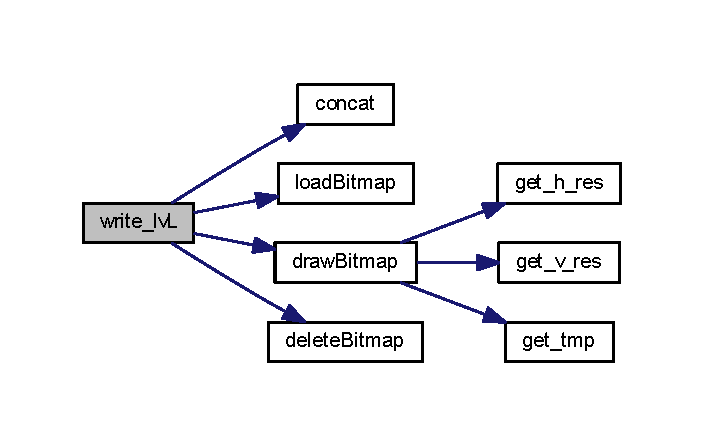
\includegraphics[width=338pt]{group__game_gaf426df873300d051272115729c8fa5a1_cgraph}
\end{center}
\end{figure}
Here is the caller graph for this function\+:
\nopagebreak
\begin{figure}[H]
\begin{center}
\leavevmode
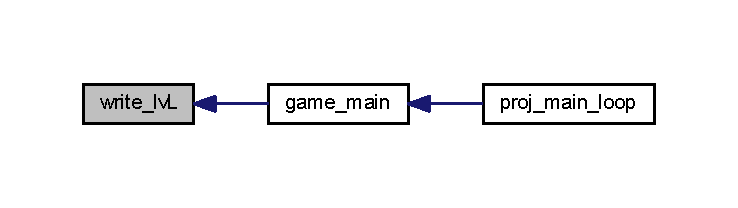
\includegraphics[width=350pt]{group__game_gaf426df873300d051272115729c8fa5a1_icgraph}
\end{center}
\end{figure}
\mbox{\Hypertarget{group__game_ga4447b1a565fed3c6130bf9e38970b933}\label{group__game_ga4447b1a565fed3c6130bf9e38970b933}} 
\index{game@{game}!write\+\_\+score@{write\+\_\+score}}
\index{write\+\_\+score@{write\+\_\+score}!game@{game}}
\subsubsection{\texorpdfstring{write\+\_\+score()}{write\_score()}}
{\footnotesize\ttfamily void write\+\_\+score (\begin{DoxyParamCaption}\item[{int}]{pont,  }\item[{\mbox{\hyperlink{structpnt}{pnt}} $\ast$}]{u,  }\item[{int}]{x,  }\item[{int}]{y }\end{DoxyParamCaption})}



Writes the score on the screen and in the game end. 


\begin{DoxyParams}{Parameters}
{\em pont} & -\/ The score obtained by the user \\
\hline
{\em u} & -\/ Pointer to the struct in which is stored the bitmap of the score \\
\hline
{\em x} & -\/ The x coordinate to place the score \\
\hline
{\em y} & -\/ The y coordinate to place the score \\
\hline
\end{DoxyParams}
Here is the call graph for this function\+:
\nopagebreak
\begin{figure}[H]
\begin{center}
\leavevmode
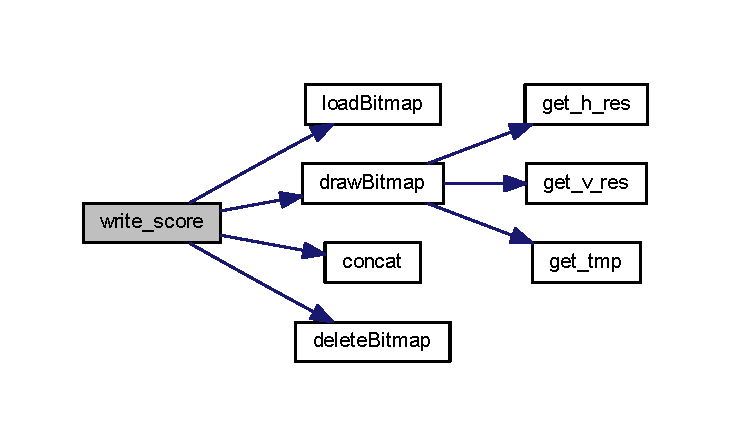
\includegraphics[width=350pt]{group__game_ga4447b1a565fed3c6130bf9e38970b933_cgraph}
\end{center}
\end{figure}
Here is the caller graph for this function\+:
\nopagebreak
\begin{figure}[H]
\begin{center}
\leavevmode
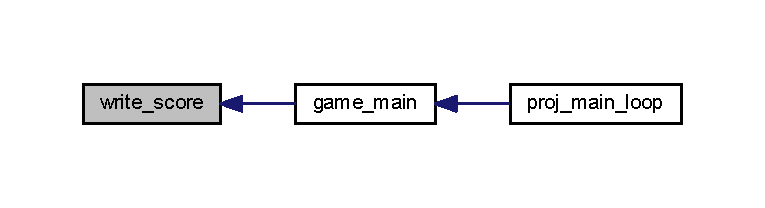
\includegraphics[width=350pt]{group__game_ga4447b1a565fed3c6130bf9e38970b933_icgraph}
\end{center}
\end{figure}


\subsection{Variable Documentation}
\mbox{\Hypertarget{group__game_ga801bef0ab9d72c95bc5d6d6a0d8f2db0}\label{group__game_ga801bef0ab9d72c95bc5d6d6a0d8f2db0}} 
\index{game@{game}!image@{image}}
\index{image@{image}!game@{game}}
\subsubsection{\texorpdfstring{image}{image}\hspace{0.1cm}{\footnotesize\ttfamily [1/7]}}
{\footnotesize\ttfamily \mbox{\hyperlink{struct_bitmap}{Bitmap}}$\ast$ image}

\mbox{\Hypertarget{group__game_ga801bef0ab9d72c95bc5d6d6a0d8f2db0}\label{group__game_ga801bef0ab9d72c95bc5d6d6a0d8f2db0}} 
\index{game@{game}!image@{image}}
\index{image@{image}!game@{game}}
\subsubsection{\texorpdfstring{image}{image}\hspace{0.1cm}{\footnotesize\ttfamily [2/7]}}
{\footnotesize\ttfamily \mbox{\hyperlink{struct_bitmap}{Bitmap}}$\ast$ image}

\mbox{\Hypertarget{group__game_ga801bef0ab9d72c95bc5d6d6a0d8f2db0}\label{group__game_ga801bef0ab9d72c95bc5d6d6a0d8f2db0}} 
\index{game@{game}!image@{image}}
\index{image@{image}!game@{game}}
\subsubsection{\texorpdfstring{image}{image}\hspace{0.1cm}{\footnotesize\ttfamily [3/7]}}
{\footnotesize\ttfamily \mbox{\hyperlink{struct_bitmap}{Bitmap}}$\ast$ image}

\mbox{\Hypertarget{group__game_ga801bef0ab9d72c95bc5d6d6a0d8f2db0}\label{group__game_ga801bef0ab9d72c95bc5d6d6a0d8f2db0}} 
\index{game@{game}!image@{image}}
\index{image@{image}!game@{game}}
\subsubsection{\texorpdfstring{image}{image}\hspace{0.1cm}{\footnotesize\ttfamily [4/7]}}
{\footnotesize\ttfamily \mbox{\hyperlink{struct_bitmap}{Bitmap}}$\ast$ image}

\mbox{\Hypertarget{group__game_ga801bef0ab9d72c95bc5d6d6a0d8f2db0}\label{group__game_ga801bef0ab9d72c95bc5d6d6a0d8f2db0}} 
\index{game@{game}!image@{image}}
\index{image@{image}!game@{game}}
\subsubsection{\texorpdfstring{image}{image}\hspace{0.1cm}{\footnotesize\ttfamily [5/7]}}
{\footnotesize\ttfamily \mbox{\hyperlink{struct_bitmap}{Bitmap}}$\ast$ image}

\mbox{\Hypertarget{group__game_ga801bef0ab9d72c95bc5d6d6a0d8f2db0}\label{group__game_ga801bef0ab9d72c95bc5d6d6a0d8f2db0}} 
\index{game@{game}!image@{image}}
\index{image@{image}!game@{game}}
\subsubsection{\texorpdfstring{image}{image}\hspace{0.1cm}{\footnotesize\ttfamily [6/7]}}
{\footnotesize\ttfamily \mbox{\hyperlink{struct_bitmap}{Bitmap}}$\ast$ image}

\mbox{\Hypertarget{group__game_ga801bef0ab9d72c95bc5d6d6a0d8f2db0}\label{group__game_ga801bef0ab9d72c95bc5d6d6a0d8f2db0}} 
\index{game@{game}!image@{image}}
\index{image@{image}!game@{game}}
\subsubsection{\texorpdfstring{image}{image}\hspace{0.1cm}{\footnotesize\ttfamily [7/7]}}
{\footnotesize\ttfamily \mbox{\hyperlink{struct_bitmap}{Bitmap}}$\ast$ image}


\hypertarget{group__i8042}{}\section{i8042}
\label{group__i8042}\index{i8042@{i8042}}
\subsection*{Macros}
\begin{DoxyCompactItemize}
\item 
\#define \mbox{\hyperlink{group__i8042_ga2d17911b50c0aeebb2e3325c5b36d4f2}{K\+E\+Y\+B\+O\+A\+R\+D\+\_\+\+I\+RQ}}~1
\item 
\#define \mbox{\hyperlink{group__i8042_ga85964cb90343bb1a029b1d1b4229f910}{M\+O\+U\+S\+E\+\_\+\+I\+RQ}}~12
\item 
\#define \mbox{\hyperlink{group__i8042_ga89c4d098b53809674457b1660b1af780}{S\+T\+A\+T\+\_\+\+R\+EG}}~0x64
\item 
\#define \mbox{\hyperlink{group__i8042_ga87da1954d01adc893f21e25bdfd48630}{I\+N\+\_\+\+B\+U\+F\+\_\+\+C\+MD}}~0x64
\item 
\#define \mbox{\hyperlink{group__i8042_ga67a4b3af0329557ddaf60c0ee0c4d906}{I\+N\+\_\+\+B\+U\+F\+\_\+\+A\+RG}}~0x60
\item 
\#define \mbox{\hyperlink{group__i8042_gacfb42dde389e8ca36ab267002fbf5c6a}{O\+U\+T\+\_\+\+B\+UF}}~0x60
\item 
\#define \mbox{\hyperlink{group__i8042_gac954b7c022e8d5b3d04300259313051e}{T\+W\+O\+\_\+\+B\+\_\+\+C\+O\+DE}}~0xe0
\item 
\#define \mbox{\hyperlink{group__i8042_gac6b47609a951e77244ef2be1691c298a}{B\+R\+E\+A\+K\+\_\+\+C\+O\+DE}}~\mbox{\hyperlink{group__vbe_ga3a8ea58898cb58fc96013383d39f482c}{B\+IT}}(7)
\item 
\#define \mbox{\hyperlink{group__i8042_ga343f44cb034d2d2ff3438b3d45dcde1f}{E\+S\+C\+\_\+\+B\+R\+E\+AK}}~0x81
\item 
\#define \mbox{\hyperlink{group__i8042_gaa554763d6a066605edecacdea834da9b}{W\+A\+I\+T\+\_\+\+K\+BC}}~20000
\item 
\#define \mbox{\hyperlink{group__i8042_gafd63d23830ad86d01b6fff2e6c615f7e}{M\+A\+X\+\_\+\+T\+R\+I\+ES}}~5
\item 
\#define \mbox{\hyperlink{group__i8042_ga307ab71673e26ec42b28a3bca05d4cb5}{P\+A\+R\+\_\+\+E\+RR}}~\mbox{\hyperlink{group__vbe_ga3a8ea58898cb58fc96013383d39f482c}{B\+IT}}(7)
\item 
\#define \mbox{\hyperlink{group__i8042_gad16f61e2bf70f6c7685e826224ed177f}{T\+O\+\_\+\+E\+RR}}~\mbox{\hyperlink{group__vbe_ga3a8ea58898cb58fc96013383d39f482c}{B\+IT}}(6)
\item 
\#define \mbox{\hyperlink{group__i8042_gad319807c29493b0d5c6916b5e50269d8}{A\+U\+X\+\_\+\+S\+ET}}~\mbox{\hyperlink{group__vbe_ga3a8ea58898cb58fc96013383d39f482c}{B\+IT}}(5)
\item 
\#define \mbox{\hyperlink{group__i8042_ga3c48b10907056351582baf9f6478598e}{I\+BF}}~\mbox{\hyperlink{group__vbe_ga3a8ea58898cb58fc96013383d39f482c}{B\+IT}}(1)
\item 
\#define \mbox{\hyperlink{group__i8042_ga45967c9e25447ba853cf6fb4ac545fe6}{O\+BF}}~\mbox{\hyperlink{group__vbe_ga3a8ea58898cb58fc96013383d39f482c}{B\+IT}}(0)
\item 
\#define \mbox{\hyperlink{group__i8042_ga3c8f3d570f82da1110d0f57effa3112f}{R\+E\+A\+D\+\_\+\+C\+M\+D\+\_\+B}}~0x20
\item 
\#define \mbox{\hyperlink{group__i8042_ga7e8f90e986320fbd1d6f22b71d967528}{I\+S\+S\+U\+E\+\_\+\+C\+M\+D\+\_\+B}}~0x60
\item 
\#define \mbox{\hyperlink{group__i8042_ga730367445dff6b45213ac50c475b02ba}{E\+N\+\_\+\+I\+N\+T\+\_\+\+K\+BD}}~\mbox{\hyperlink{group__vbe_ga3a8ea58898cb58fc96013383d39f482c}{B\+IT}}(0)
\item 
\#define \mbox{\hyperlink{group__i8042_ga91a8577f9ccfdba456eb4cb568a35b07}{D\+I\+S\+\_\+\+C\+M\+D\+\_\+\+M\+O\+U\+SE}}~\mbox{\hyperlink{group__vbe_ga3a8ea58898cb58fc96013383d39f482c}{B\+IT}}(5)
\item 
\#define \mbox{\hyperlink{group__i8042_ga038bc8729428bdd48e35ff23538da385}{D\+I\+S\+\_\+\+K\+EY}}~\mbox{\hyperlink{group__vbe_ga3a8ea58898cb58fc96013383d39f482c}{B\+IT}}(4)
\item 
\#define \mbox{\hyperlink{group__i8042_ga48caab510032bf5e44c41f9b1e30b266}{E\+N\+\_\+\+I\+N\+T\+\_\+\+M\+O\+U\+SE}}~\mbox{\hyperlink{group__vbe_ga3a8ea58898cb58fc96013383d39f482c}{B\+IT}}(1)
\item 
\#define \mbox{\hyperlink{group__i8042_ga1ddfd048fd8ccbdc07f69723de35b3b7}{D\+I\+S\+\_\+\+I\+N\+T\+\_\+\+K\+BD}}~0x\+FE
\item 
\#define \mbox{\hyperlink{group__i8042_ga229365f650b36906bd1868ec0b0346c8}{D\+I\+S\+\_\+\+I\+N\+T\+\_\+\+M\+O\+U\+SE}}~0x\+FD
\item 
\#define \mbox{\hyperlink{group__i8042_ga77c4c69c52a0d0a44e35a72d47e083dc}{F\+L\+A\+G\+\_\+\+B\+Y\+T\+E1}}~\mbox{\hyperlink{group__vbe_ga3a8ea58898cb58fc96013383d39f482c}{B\+IT}}(3)
\item 
\#define \mbox{\hyperlink{group__i8042_gacc55daa58d88a3612f2ef74a6abbe97f}{LB}}~\mbox{\hyperlink{group__vbe_ga3a8ea58898cb58fc96013383d39f482c}{B\+IT}}(0)
\item 
\#define \mbox{\hyperlink{group__i8042_ga171160a766f85c8816b898ed24d28408}{RB}}~\mbox{\hyperlink{group__vbe_ga3a8ea58898cb58fc96013383d39f482c}{B\+IT}}(1)
\item 
\#define \mbox{\hyperlink{group__i8042_gaa6b38d492364d98453284934ed7caee9}{MB}}~\mbox{\hyperlink{group__vbe_ga3a8ea58898cb58fc96013383d39f482c}{B\+IT}}(2)
\item 
\#define \mbox{\hyperlink{group__i8042_ga181f1c2860e4d7fd7788990378061137}{X\+\_\+\+S\+I\+GN}}~\mbox{\hyperlink{group__vbe_ga3a8ea58898cb58fc96013383d39f482c}{B\+IT}}(4)
\item 
\#define \mbox{\hyperlink{group__i8042_ga2a0064e2f0979eea21b81e4fe6b2ac32}{Y\+\_\+\+S\+I\+GN}}~\mbox{\hyperlink{group__vbe_ga3a8ea58898cb58fc96013383d39f482c}{B\+IT}}(5)
\item 
\#define \mbox{\hyperlink{group__i8042_ga858379c2252a71bc12dd9ff796477d90}{X\+\_\+\+O\+VF}}~\mbox{\hyperlink{group__vbe_ga3a8ea58898cb58fc96013383d39f482c}{B\+IT}}(6)
\item 
\#define \mbox{\hyperlink{group__i8042_ga8238446128710bc20d7c73b2fa785c72}{Y\+\_\+\+O\+VF}}~\mbox{\hyperlink{group__vbe_ga3a8ea58898cb58fc96013383d39f482c}{B\+IT}}(7)
\item 
\#define \mbox{\hyperlink{group__i8042_gaec49e28277af866462cbe6e426a120ef}{D\+I\+S\+\_\+\+M\+O\+U\+SE}}~0x\+A7
\item 
\#define \mbox{\hyperlink{group__i8042_gaf9776e4566c3a77a7c3631530998f386}{E\+N\+\_\+\+M\+O\+U\+SE}}~0x\+A8
\item 
\#define \mbox{\hyperlink{group__i8042_gae3d0f97115be6f01d0ad43399f709868}{C\+H\+E\+C\+K\+\_\+\+M\+O\+U\+S\+E\+\_\+\+I\+NT}}~0x\+A9
\item 
\#define \mbox{\hyperlink{group__i8042_gaa0b21fb358640f27c94090e845b497ae}{I\+S\+S\+U\+E\+\_\+\+B\+Y2\+M\+O\+U\+SE}}~0x\+D4
\item 
\#define \mbox{\hyperlink{group__i8042_ga9316ae006907490c32654ca0248e678a}{E\+N\+\_\+\+D\+A\+T\+A\+\_\+\+R\+EP}}~0x\+F4
\item 
\#define \mbox{\hyperlink{group__i8042_ga1c84607e844d7b3736a1a3491c18e872}{D\+I\+S\+\_\+\+D\+A\+T\+A\+\_\+\+R\+EP}}~0\+X\+F5
\item 
\#define \mbox{\hyperlink{group__i8042_gab3919f33b46e0808c4ed1c56a6a423f2}{S\+T\+R\+E\+A\+M\+\_\+\+M\+O\+DE}}~0x\+EA
\item 
\#define \mbox{\hyperlink{group__i8042_ga17981ca5836957abd2dfe6b77d96744d}{R\+E\+M\+O\+T\+E\+\_\+\+M\+O\+DE}}~0x\+F0
\item 
\#define \mbox{\hyperlink{group__i8042_ga8d406d5aff787991429e62cfd9bac721}{R\+E\+A\+D\+\_\+\+D\+A\+TA}}~0x\+EB
\item 
\#define \mbox{\hyperlink{group__i8042_ga6f6489887e08bff4887d0bc5dcf214d8}{A\+CK}}~0x\+FA
\item 
\#define \mbox{\hyperlink{group__i8042_ga958518a45b12053ae33606ee7cb68a55}{N\+A\+CK}}~0x\+FE
\item 
\#define \mbox{\hyperlink{group__i8042_ga8fe83ac76edc595f6b98cd4a4127aed5}{E\+R\+R\+OR}}~0x\+FC
\end{DoxyCompactItemize}


\subsection{Detailed Description}
Constants for programming the i8254 kbc. 

\subsection{Macro Definition Documentation}
\mbox{\Hypertarget{group__i8042_ga6f6489887e08bff4887d0bc5dcf214d8}\label{group__i8042_ga6f6489887e08bff4887d0bc5dcf214d8}} 
\index{i8042@{i8042}!A\+CK@{A\+CK}}
\index{A\+CK@{A\+CK}!i8042@{i8042}}
\subsubsection{\texorpdfstring{A\+CK}{ACK}}
{\footnotesize\ttfamily \#define A\+CK~0x\+FA}

\mbox{\Hypertarget{group__i8042_gad319807c29493b0d5c6916b5e50269d8}\label{group__i8042_gad319807c29493b0d5c6916b5e50269d8}} 
\index{i8042@{i8042}!A\+U\+X\+\_\+\+S\+ET@{A\+U\+X\+\_\+\+S\+ET}}
\index{A\+U\+X\+\_\+\+S\+ET@{A\+U\+X\+\_\+\+S\+ET}!i8042@{i8042}}
\subsubsection{\texorpdfstring{A\+U\+X\+\_\+\+S\+ET}{AUX\_SET}}
{\footnotesize\ttfamily \#define A\+U\+X\+\_\+\+S\+ET~\mbox{\hyperlink{group__vbe_ga3a8ea58898cb58fc96013383d39f482c}{B\+IT}}(5)}

\mbox{\Hypertarget{group__i8042_gac6b47609a951e77244ef2be1691c298a}\label{group__i8042_gac6b47609a951e77244ef2be1691c298a}} 
\index{i8042@{i8042}!B\+R\+E\+A\+K\+\_\+\+C\+O\+DE@{B\+R\+E\+A\+K\+\_\+\+C\+O\+DE}}
\index{B\+R\+E\+A\+K\+\_\+\+C\+O\+DE@{B\+R\+E\+A\+K\+\_\+\+C\+O\+DE}!i8042@{i8042}}
\subsubsection{\texorpdfstring{B\+R\+E\+A\+K\+\_\+\+C\+O\+DE}{BREAK\_CODE}}
{\footnotesize\ttfamily \#define B\+R\+E\+A\+K\+\_\+\+C\+O\+DE~\mbox{\hyperlink{group__vbe_ga3a8ea58898cb58fc96013383d39f482c}{B\+IT}}(7)}

\mbox{\Hypertarget{group__i8042_gae3d0f97115be6f01d0ad43399f709868}\label{group__i8042_gae3d0f97115be6f01d0ad43399f709868}} 
\index{i8042@{i8042}!C\+H\+E\+C\+K\+\_\+\+M\+O\+U\+S\+E\+\_\+\+I\+NT@{C\+H\+E\+C\+K\+\_\+\+M\+O\+U\+S\+E\+\_\+\+I\+NT}}
\index{C\+H\+E\+C\+K\+\_\+\+M\+O\+U\+S\+E\+\_\+\+I\+NT@{C\+H\+E\+C\+K\+\_\+\+M\+O\+U\+S\+E\+\_\+\+I\+NT}!i8042@{i8042}}
\subsubsection{\texorpdfstring{C\+H\+E\+C\+K\+\_\+\+M\+O\+U\+S\+E\+\_\+\+I\+NT}{CHECK\_MOUSE\_INT}}
{\footnotesize\ttfamily \#define C\+H\+E\+C\+K\+\_\+\+M\+O\+U\+S\+E\+\_\+\+I\+NT~0x\+A9}

\mbox{\Hypertarget{group__i8042_ga91a8577f9ccfdba456eb4cb568a35b07}\label{group__i8042_ga91a8577f9ccfdba456eb4cb568a35b07}} 
\index{i8042@{i8042}!D\+I\+S\+\_\+\+C\+M\+D\+\_\+\+M\+O\+U\+SE@{D\+I\+S\+\_\+\+C\+M\+D\+\_\+\+M\+O\+U\+SE}}
\index{D\+I\+S\+\_\+\+C\+M\+D\+\_\+\+M\+O\+U\+SE@{D\+I\+S\+\_\+\+C\+M\+D\+\_\+\+M\+O\+U\+SE}!i8042@{i8042}}
\subsubsection{\texorpdfstring{D\+I\+S\+\_\+\+C\+M\+D\+\_\+\+M\+O\+U\+SE}{DIS\_CMD\_MOUSE}}
{\footnotesize\ttfamily \#define D\+I\+S\+\_\+\+C\+M\+D\+\_\+\+M\+O\+U\+SE~\mbox{\hyperlink{group__vbe_ga3a8ea58898cb58fc96013383d39f482c}{B\+IT}}(5)}

\mbox{\Hypertarget{group__i8042_ga1c84607e844d7b3736a1a3491c18e872}\label{group__i8042_ga1c84607e844d7b3736a1a3491c18e872}} 
\index{i8042@{i8042}!D\+I\+S\+\_\+\+D\+A\+T\+A\+\_\+\+R\+EP@{D\+I\+S\+\_\+\+D\+A\+T\+A\+\_\+\+R\+EP}}
\index{D\+I\+S\+\_\+\+D\+A\+T\+A\+\_\+\+R\+EP@{D\+I\+S\+\_\+\+D\+A\+T\+A\+\_\+\+R\+EP}!i8042@{i8042}}
\subsubsection{\texorpdfstring{D\+I\+S\+\_\+\+D\+A\+T\+A\+\_\+\+R\+EP}{DIS\_DATA\_REP}}
{\footnotesize\ttfamily \#define D\+I\+S\+\_\+\+D\+A\+T\+A\+\_\+\+R\+EP~0\+X\+F5}

\mbox{\Hypertarget{group__i8042_ga1ddfd048fd8ccbdc07f69723de35b3b7}\label{group__i8042_ga1ddfd048fd8ccbdc07f69723de35b3b7}} 
\index{i8042@{i8042}!D\+I\+S\+\_\+\+I\+N\+T\+\_\+\+K\+BD@{D\+I\+S\+\_\+\+I\+N\+T\+\_\+\+K\+BD}}
\index{D\+I\+S\+\_\+\+I\+N\+T\+\_\+\+K\+BD@{D\+I\+S\+\_\+\+I\+N\+T\+\_\+\+K\+BD}!i8042@{i8042}}
\subsubsection{\texorpdfstring{D\+I\+S\+\_\+\+I\+N\+T\+\_\+\+K\+BD}{DIS\_INT\_KBD}}
{\footnotesize\ttfamily \#define D\+I\+S\+\_\+\+I\+N\+T\+\_\+\+K\+BD~0x\+FE}

\mbox{\Hypertarget{group__i8042_ga229365f650b36906bd1868ec0b0346c8}\label{group__i8042_ga229365f650b36906bd1868ec0b0346c8}} 
\index{i8042@{i8042}!D\+I\+S\+\_\+\+I\+N\+T\+\_\+\+M\+O\+U\+SE@{D\+I\+S\+\_\+\+I\+N\+T\+\_\+\+M\+O\+U\+SE}}
\index{D\+I\+S\+\_\+\+I\+N\+T\+\_\+\+M\+O\+U\+SE@{D\+I\+S\+\_\+\+I\+N\+T\+\_\+\+M\+O\+U\+SE}!i8042@{i8042}}
\subsubsection{\texorpdfstring{D\+I\+S\+\_\+\+I\+N\+T\+\_\+\+M\+O\+U\+SE}{DIS\_INT\_MOUSE}}
{\footnotesize\ttfamily \#define D\+I\+S\+\_\+\+I\+N\+T\+\_\+\+M\+O\+U\+SE~0x\+FD}

\mbox{\Hypertarget{group__i8042_ga038bc8729428bdd48e35ff23538da385}\label{group__i8042_ga038bc8729428bdd48e35ff23538da385}} 
\index{i8042@{i8042}!D\+I\+S\+\_\+\+K\+EY@{D\+I\+S\+\_\+\+K\+EY}}
\index{D\+I\+S\+\_\+\+K\+EY@{D\+I\+S\+\_\+\+K\+EY}!i8042@{i8042}}
\subsubsection{\texorpdfstring{D\+I\+S\+\_\+\+K\+EY}{DIS\_KEY}}
{\footnotesize\ttfamily \#define D\+I\+S\+\_\+\+K\+EY~\mbox{\hyperlink{group__vbe_ga3a8ea58898cb58fc96013383d39f482c}{B\+IT}}(4)}

\mbox{\Hypertarget{group__i8042_gaec49e28277af866462cbe6e426a120ef}\label{group__i8042_gaec49e28277af866462cbe6e426a120ef}} 
\index{i8042@{i8042}!D\+I\+S\+\_\+\+M\+O\+U\+SE@{D\+I\+S\+\_\+\+M\+O\+U\+SE}}
\index{D\+I\+S\+\_\+\+M\+O\+U\+SE@{D\+I\+S\+\_\+\+M\+O\+U\+SE}!i8042@{i8042}}
\subsubsection{\texorpdfstring{D\+I\+S\+\_\+\+M\+O\+U\+SE}{DIS\_MOUSE}}
{\footnotesize\ttfamily \#define D\+I\+S\+\_\+\+M\+O\+U\+SE~0x\+A7}

\mbox{\Hypertarget{group__i8042_ga9316ae006907490c32654ca0248e678a}\label{group__i8042_ga9316ae006907490c32654ca0248e678a}} 
\index{i8042@{i8042}!E\+N\+\_\+\+D\+A\+T\+A\+\_\+\+R\+EP@{E\+N\+\_\+\+D\+A\+T\+A\+\_\+\+R\+EP}}
\index{E\+N\+\_\+\+D\+A\+T\+A\+\_\+\+R\+EP@{E\+N\+\_\+\+D\+A\+T\+A\+\_\+\+R\+EP}!i8042@{i8042}}
\subsubsection{\texorpdfstring{E\+N\+\_\+\+D\+A\+T\+A\+\_\+\+R\+EP}{EN\_DATA\_REP}}
{\footnotesize\ttfamily \#define E\+N\+\_\+\+D\+A\+T\+A\+\_\+\+R\+EP~0x\+F4}

\mbox{\Hypertarget{group__i8042_ga730367445dff6b45213ac50c475b02ba}\label{group__i8042_ga730367445dff6b45213ac50c475b02ba}} 
\index{i8042@{i8042}!E\+N\+\_\+\+I\+N\+T\+\_\+\+K\+BD@{E\+N\+\_\+\+I\+N\+T\+\_\+\+K\+BD}}
\index{E\+N\+\_\+\+I\+N\+T\+\_\+\+K\+BD@{E\+N\+\_\+\+I\+N\+T\+\_\+\+K\+BD}!i8042@{i8042}}
\subsubsection{\texorpdfstring{E\+N\+\_\+\+I\+N\+T\+\_\+\+K\+BD}{EN\_INT\_KBD}}
{\footnotesize\ttfamily \#define E\+N\+\_\+\+I\+N\+T\+\_\+\+K\+BD~\mbox{\hyperlink{group__vbe_ga3a8ea58898cb58fc96013383d39f482c}{B\+IT}}(0)}

\mbox{\Hypertarget{group__i8042_ga48caab510032bf5e44c41f9b1e30b266}\label{group__i8042_ga48caab510032bf5e44c41f9b1e30b266}} 
\index{i8042@{i8042}!E\+N\+\_\+\+I\+N\+T\+\_\+\+M\+O\+U\+SE@{E\+N\+\_\+\+I\+N\+T\+\_\+\+M\+O\+U\+SE}}
\index{E\+N\+\_\+\+I\+N\+T\+\_\+\+M\+O\+U\+SE@{E\+N\+\_\+\+I\+N\+T\+\_\+\+M\+O\+U\+SE}!i8042@{i8042}}
\subsubsection{\texorpdfstring{E\+N\+\_\+\+I\+N\+T\+\_\+\+M\+O\+U\+SE}{EN\_INT\_MOUSE}}
{\footnotesize\ttfamily \#define E\+N\+\_\+\+I\+N\+T\+\_\+\+M\+O\+U\+SE~\mbox{\hyperlink{group__vbe_ga3a8ea58898cb58fc96013383d39f482c}{B\+IT}}(1)}

\mbox{\Hypertarget{group__i8042_gaf9776e4566c3a77a7c3631530998f386}\label{group__i8042_gaf9776e4566c3a77a7c3631530998f386}} 
\index{i8042@{i8042}!E\+N\+\_\+\+M\+O\+U\+SE@{E\+N\+\_\+\+M\+O\+U\+SE}}
\index{E\+N\+\_\+\+M\+O\+U\+SE@{E\+N\+\_\+\+M\+O\+U\+SE}!i8042@{i8042}}
\subsubsection{\texorpdfstring{E\+N\+\_\+\+M\+O\+U\+SE}{EN\_MOUSE}}
{\footnotesize\ttfamily \#define E\+N\+\_\+\+M\+O\+U\+SE~0x\+A8}

\mbox{\Hypertarget{group__i8042_ga8fe83ac76edc595f6b98cd4a4127aed5}\label{group__i8042_ga8fe83ac76edc595f6b98cd4a4127aed5}} 
\index{i8042@{i8042}!E\+R\+R\+OR@{E\+R\+R\+OR}}
\index{E\+R\+R\+OR@{E\+R\+R\+OR}!i8042@{i8042}}
\subsubsection{\texorpdfstring{E\+R\+R\+OR}{ERROR}}
{\footnotesize\ttfamily \#define E\+R\+R\+OR~0x\+FC}

\mbox{\Hypertarget{group__i8042_ga343f44cb034d2d2ff3438b3d45dcde1f}\label{group__i8042_ga343f44cb034d2d2ff3438b3d45dcde1f}} 
\index{i8042@{i8042}!E\+S\+C\+\_\+\+B\+R\+E\+AK@{E\+S\+C\+\_\+\+B\+R\+E\+AK}}
\index{E\+S\+C\+\_\+\+B\+R\+E\+AK@{E\+S\+C\+\_\+\+B\+R\+E\+AK}!i8042@{i8042}}
\subsubsection{\texorpdfstring{E\+S\+C\+\_\+\+B\+R\+E\+AK}{ESC\_BREAK}}
{\footnotesize\ttfamily \#define E\+S\+C\+\_\+\+B\+R\+E\+AK~0x81}

\mbox{\Hypertarget{group__i8042_ga77c4c69c52a0d0a44e35a72d47e083dc}\label{group__i8042_ga77c4c69c52a0d0a44e35a72d47e083dc}} 
\index{i8042@{i8042}!F\+L\+A\+G\+\_\+\+B\+Y\+T\+E1@{F\+L\+A\+G\+\_\+\+B\+Y\+T\+E1}}
\index{F\+L\+A\+G\+\_\+\+B\+Y\+T\+E1@{F\+L\+A\+G\+\_\+\+B\+Y\+T\+E1}!i8042@{i8042}}
\subsubsection{\texorpdfstring{F\+L\+A\+G\+\_\+\+B\+Y\+T\+E1}{FLAG\_BYTE1}}
{\footnotesize\ttfamily \#define F\+L\+A\+G\+\_\+\+B\+Y\+T\+E1~\mbox{\hyperlink{group__vbe_ga3a8ea58898cb58fc96013383d39f482c}{B\+IT}}(3)}

\mbox{\Hypertarget{group__i8042_ga3c48b10907056351582baf9f6478598e}\label{group__i8042_ga3c48b10907056351582baf9f6478598e}} 
\index{i8042@{i8042}!I\+BF@{I\+BF}}
\index{I\+BF@{I\+BF}!i8042@{i8042}}
\subsubsection{\texorpdfstring{I\+BF}{IBF}}
{\footnotesize\ttfamily \#define I\+BF~\mbox{\hyperlink{group__vbe_ga3a8ea58898cb58fc96013383d39f482c}{B\+IT}}(1)}

\mbox{\Hypertarget{group__i8042_ga67a4b3af0329557ddaf60c0ee0c4d906}\label{group__i8042_ga67a4b3af0329557ddaf60c0ee0c4d906}} 
\index{i8042@{i8042}!I\+N\+\_\+\+B\+U\+F\+\_\+\+A\+RG@{I\+N\+\_\+\+B\+U\+F\+\_\+\+A\+RG}}
\index{I\+N\+\_\+\+B\+U\+F\+\_\+\+A\+RG@{I\+N\+\_\+\+B\+U\+F\+\_\+\+A\+RG}!i8042@{i8042}}
\subsubsection{\texorpdfstring{I\+N\+\_\+\+B\+U\+F\+\_\+\+A\+RG}{IN\_BUF\_ARG}}
{\footnotesize\ttfamily \#define I\+N\+\_\+\+B\+U\+F\+\_\+\+A\+RG~0x60}

\mbox{\Hypertarget{group__i8042_ga87da1954d01adc893f21e25bdfd48630}\label{group__i8042_ga87da1954d01adc893f21e25bdfd48630}} 
\index{i8042@{i8042}!I\+N\+\_\+\+B\+U\+F\+\_\+\+C\+MD@{I\+N\+\_\+\+B\+U\+F\+\_\+\+C\+MD}}
\index{I\+N\+\_\+\+B\+U\+F\+\_\+\+C\+MD@{I\+N\+\_\+\+B\+U\+F\+\_\+\+C\+MD}!i8042@{i8042}}
\subsubsection{\texorpdfstring{I\+N\+\_\+\+B\+U\+F\+\_\+\+C\+MD}{IN\_BUF\_CMD}}
{\footnotesize\ttfamily \#define I\+N\+\_\+\+B\+U\+F\+\_\+\+C\+MD~0x64}

\mbox{\Hypertarget{group__i8042_gaa0b21fb358640f27c94090e845b497ae}\label{group__i8042_gaa0b21fb358640f27c94090e845b497ae}} 
\index{i8042@{i8042}!I\+S\+S\+U\+E\+\_\+\+B\+Y2\+M\+O\+U\+SE@{I\+S\+S\+U\+E\+\_\+\+B\+Y2\+M\+O\+U\+SE}}
\index{I\+S\+S\+U\+E\+\_\+\+B\+Y2\+M\+O\+U\+SE@{I\+S\+S\+U\+E\+\_\+\+B\+Y2\+M\+O\+U\+SE}!i8042@{i8042}}
\subsubsection{\texorpdfstring{I\+S\+S\+U\+E\+\_\+\+B\+Y2\+M\+O\+U\+SE}{ISSUE\_BY2MOUSE}}
{\footnotesize\ttfamily \#define I\+S\+S\+U\+E\+\_\+\+B\+Y2\+M\+O\+U\+SE~0x\+D4}

\mbox{\Hypertarget{group__i8042_ga7e8f90e986320fbd1d6f22b71d967528}\label{group__i8042_ga7e8f90e986320fbd1d6f22b71d967528}} 
\index{i8042@{i8042}!I\+S\+S\+U\+E\+\_\+\+C\+M\+D\+\_\+B@{I\+S\+S\+U\+E\+\_\+\+C\+M\+D\+\_\+B}}
\index{I\+S\+S\+U\+E\+\_\+\+C\+M\+D\+\_\+B@{I\+S\+S\+U\+E\+\_\+\+C\+M\+D\+\_\+B}!i8042@{i8042}}
\subsubsection{\texorpdfstring{I\+S\+S\+U\+E\+\_\+\+C\+M\+D\+\_\+B}{ISSUE\_CMD\_B}}
{\footnotesize\ttfamily \#define I\+S\+S\+U\+E\+\_\+\+C\+M\+D\+\_\+B~0x60}

\mbox{\Hypertarget{group__i8042_ga2d17911b50c0aeebb2e3325c5b36d4f2}\label{group__i8042_ga2d17911b50c0aeebb2e3325c5b36d4f2}} 
\index{i8042@{i8042}!K\+E\+Y\+B\+O\+A\+R\+D\+\_\+\+I\+RQ@{K\+E\+Y\+B\+O\+A\+R\+D\+\_\+\+I\+RQ}}
\index{K\+E\+Y\+B\+O\+A\+R\+D\+\_\+\+I\+RQ@{K\+E\+Y\+B\+O\+A\+R\+D\+\_\+\+I\+RQ}!i8042@{i8042}}
\subsubsection{\texorpdfstring{K\+E\+Y\+B\+O\+A\+R\+D\+\_\+\+I\+RQ}{KEYBOARD\_IRQ}}
{\footnotesize\ttfamily \#define K\+E\+Y\+B\+O\+A\+R\+D\+\_\+\+I\+RQ~1}

\mbox{\Hypertarget{group__i8042_gacc55daa58d88a3612f2ef74a6abbe97f}\label{group__i8042_gacc55daa58d88a3612f2ef74a6abbe97f}} 
\index{i8042@{i8042}!LB@{LB}}
\index{LB@{LB}!i8042@{i8042}}
\subsubsection{\texorpdfstring{LB}{LB}}
{\footnotesize\ttfamily \#define LB~\mbox{\hyperlink{group__vbe_ga3a8ea58898cb58fc96013383d39f482c}{B\+IT}}(0)}

\mbox{\Hypertarget{group__i8042_gafd63d23830ad86d01b6fff2e6c615f7e}\label{group__i8042_gafd63d23830ad86d01b6fff2e6c615f7e}} 
\index{i8042@{i8042}!M\+A\+X\+\_\+\+T\+R\+I\+ES@{M\+A\+X\+\_\+\+T\+R\+I\+ES}}
\index{M\+A\+X\+\_\+\+T\+R\+I\+ES@{M\+A\+X\+\_\+\+T\+R\+I\+ES}!i8042@{i8042}}
\subsubsection{\texorpdfstring{M\+A\+X\+\_\+\+T\+R\+I\+ES}{MAX\_TRIES}}
{\footnotesize\ttfamily \#define M\+A\+X\+\_\+\+T\+R\+I\+ES~5}

\mbox{\Hypertarget{group__i8042_gaa6b38d492364d98453284934ed7caee9}\label{group__i8042_gaa6b38d492364d98453284934ed7caee9}} 
\index{i8042@{i8042}!MB@{MB}}
\index{MB@{MB}!i8042@{i8042}}
\subsubsection{\texorpdfstring{MB}{MB}}
{\footnotesize\ttfamily \#define MB~\mbox{\hyperlink{group__vbe_ga3a8ea58898cb58fc96013383d39f482c}{B\+IT}}(2)}

\mbox{\Hypertarget{group__i8042_ga85964cb90343bb1a029b1d1b4229f910}\label{group__i8042_ga85964cb90343bb1a029b1d1b4229f910}} 
\index{i8042@{i8042}!M\+O\+U\+S\+E\+\_\+\+I\+RQ@{M\+O\+U\+S\+E\+\_\+\+I\+RQ}}
\index{M\+O\+U\+S\+E\+\_\+\+I\+RQ@{M\+O\+U\+S\+E\+\_\+\+I\+RQ}!i8042@{i8042}}
\subsubsection{\texorpdfstring{M\+O\+U\+S\+E\+\_\+\+I\+RQ}{MOUSE\_IRQ}}
{\footnotesize\ttfamily \#define M\+O\+U\+S\+E\+\_\+\+I\+RQ~12}

\mbox{\Hypertarget{group__i8042_ga958518a45b12053ae33606ee7cb68a55}\label{group__i8042_ga958518a45b12053ae33606ee7cb68a55}} 
\index{i8042@{i8042}!N\+A\+CK@{N\+A\+CK}}
\index{N\+A\+CK@{N\+A\+CK}!i8042@{i8042}}
\subsubsection{\texorpdfstring{N\+A\+CK}{NACK}}
{\footnotesize\ttfamily \#define N\+A\+CK~0x\+FE}

\mbox{\Hypertarget{group__i8042_ga45967c9e25447ba853cf6fb4ac545fe6}\label{group__i8042_ga45967c9e25447ba853cf6fb4ac545fe6}} 
\index{i8042@{i8042}!O\+BF@{O\+BF}}
\index{O\+BF@{O\+BF}!i8042@{i8042}}
\subsubsection{\texorpdfstring{O\+BF}{OBF}}
{\footnotesize\ttfamily \#define O\+BF~\mbox{\hyperlink{group__vbe_ga3a8ea58898cb58fc96013383d39f482c}{B\+IT}}(0)}

\mbox{\Hypertarget{group__i8042_gacfb42dde389e8ca36ab267002fbf5c6a}\label{group__i8042_gacfb42dde389e8ca36ab267002fbf5c6a}} 
\index{i8042@{i8042}!O\+U\+T\+\_\+\+B\+UF@{O\+U\+T\+\_\+\+B\+UF}}
\index{O\+U\+T\+\_\+\+B\+UF@{O\+U\+T\+\_\+\+B\+UF}!i8042@{i8042}}
\subsubsection{\texorpdfstring{O\+U\+T\+\_\+\+B\+UF}{OUT\_BUF}}
{\footnotesize\ttfamily \#define O\+U\+T\+\_\+\+B\+UF~0x60}

\mbox{\Hypertarget{group__i8042_ga307ab71673e26ec42b28a3bca05d4cb5}\label{group__i8042_ga307ab71673e26ec42b28a3bca05d4cb5}} 
\index{i8042@{i8042}!P\+A\+R\+\_\+\+E\+RR@{P\+A\+R\+\_\+\+E\+RR}}
\index{P\+A\+R\+\_\+\+E\+RR@{P\+A\+R\+\_\+\+E\+RR}!i8042@{i8042}}
\subsubsection{\texorpdfstring{P\+A\+R\+\_\+\+E\+RR}{PAR\_ERR}}
{\footnotesize\ttfamily \#define P\+A\+R\+\_\+\+E\+RR~\mbox{\hyperlink{group__vbe_ga3a8ea58898cb58fc96013383d39f482c}{B\+IT}}(7)}

\mbox{\Hypertarget{group__i8042_ga171160a766f85c8816b898ed24d28408}\label{group__i8042_ga171160a766f85c8816b898ed24d28408}} 
\index{i8042@{i8042}!RB@{RB}}
\index{RB@{RB}!i8042@{i8042}}
\subsubsection{\texorpdfstring{RB}{RB}}
{\footnotesize\ttfamily \#define RB~\mbox{\hyperlink{group__vbe_ga3a8ea58898cb58fc96013383d39f482c}{B\+IT}}(1)}

\mbox{\Hypertarget{group__i8042_ga3c8f3d570f82da1110d0f57effa3112f}\label{group__i8042_ga3c8f3d570f82da1110d0f57effa3112f}} 
\index{i8042@{i8042}!R\+E\+A\+D\+\_\+\+C\+M\+D\+\_\+B@{R\+E\+A\+D\+\_\+\+C\+M\+D\+\_\+B}}
\index{R\+E\+A\+D\+\_\+\+C\+M\+D\+\_\+B@{R\+E\+A\+D\+\_\+\+C\+M\+D\+\_\+B}!i8042@{i8042}}
\subsubsection{\texorpdfstring{R\+E\+A\+D\+\_\+\+C\+M\+D\+\_\+B}{READ\_CMD\_B}}
{\footnotesize\ttfamily \#define R\+E\+A\+D\+\_\+\+C\+M\+D\+\_\+B~0x20}

\mbox{\Hypertarget{group__i8042_ga8d406d5aff787991429e62cfd9bac721}\label{group__i8042_ga8d406d5aff787991429e62cfd9bac721}} 
\index{i8042@{i8042}!R\+E\+A\+D\+\_\+\+D\+A\+TA@{R\+E\+A\+D\+\_\+\+D\+A\+TA}}
\index{R\+E\+A\+D\+\_\+\+D\+A\+TA@{R\+E\+A\+D\+\_\+\+D\+A\+TA}!i8042@{i8042}}
\subsubsection{\texorpdfstring{R\+E\+A\+D\+\_\+\+D\+A\+TA}{READ\_DATA}}
{\footnotesize\ttfamily \#define R\+E\+A\+D\+\_\+\+D\+A\+TA~0x\+EB}

\mbox{\Hypertarget{group__i8042_ga17981ca5836957abd2dfe6b77d96744d}\label{group__i8042_ga17981ca5836957abd2dfe6b77d96744d}} 
\index{i8042@{i8042}!R\+E\+M\+O\+T\+E\+\_\+\+M\+O\+DE@{R\+E\+M\+O\+T\+E\+\_\+\+M\+O\+DE}}
\index{R\+E\+M\+O\+T\+E\+\_\+\+M\+O\+DE@{R\+E\+M\+O\+T\+E\+\_\+\+M\+O\+DE}!i8042@{i8042}}
\subsubsection{\texorpdfstring{R\+E\+M\+O\+T\+E\+\_\+\+M\+O\+DE}{REMOTE\_MODE}}
{\footnotesize\ttfamily \#define R\+E\+M\+O\+T\+E\+\_\+\+M\+O\+DE~0x\+F0}

\mbox{\Hypertarget{group__i8042_ga89c4d098b53809674457b1660b1af780}\label{group__i8042_ga89c4d098b53809674457b1660b1af780}} 
\index{i8042@{i8042}!S\+T\+A\+T\+\_\+\+R\+EG@{S\+T\+A\+T\+\_\+\+R\+EG}}
\index{S\+T\+A\+T\+\_\+\+R\+EG@{S\+T\+A\+T\+\_\+\+R\+EG}!i8042@{i8042}}
\subsubsection{\texorpdfstring{S\+T\+A\+T\+\_\+\+R\+EG}{STAT\_REG}}
{\footnotesize\ttfamily \#define S\+T\+A\+T\+\_\+\+R\+EG~0x64}

\mbox{\Hypertarget{group__i8042_gab3919f33b46e0808c4ed1c56a6a423f2}\label{group__i8042_gab3919f33b46e0808c4ed1c56a6a423f2}} 
\index{i8042@{i8042}!S\+T\+R\+E\+A\+M\+\_\+\+M\+O\+DE@{S\+T\+R\+E\+A\+M\+\_\+\+M\+O\+DE}}
\index{S\+T\+R\+E\+A\+M\+\_\+\+M\+O\+DE@{S\+T\+R\+E\+A\+M\+\_\+\+M\+O\+DE}!i8042@{i8042}}
\subsubsection{\texorpdfstring{S\+T\+R\+E\+A\+M\+\_\+\+M\+O\+DE}{STREAM\_MODE}}
{\footnotesize\ttfamily \#define S\+T\+R\+E\+A\+M\+\_\+\+M\+O\+DE~0x\+EA}

\mbox{\Hypertarget{group__i8042_gad16f61e2bf70f6c7685e826224ed177f}\label{group__i8042_gad16f61e2bf70f6c7685e826224ed177f}} 
\index{i8042@{i8042}!T\+O\+\_\+\+E\+RR@{T\+O\+\_\+\+E\+RR}}
\index{T\+O\+\_\+\+E\+RR@{T\+O\+\_\+\+E\+RR}!i8042@{i8042}}
\subsubsection{\texorpdfstring{T\+O\+\_\+\+E\+RR}{TO\_ERR}}
{\footnotesize\ttfamily \#define T\+O\+\_\+\+E\+RR~\mbox{\hyperlink{group__vbe_ga3a8ea58898cb58fc96013383d39f482c}{B\+IT}}(6)}

\mbox{\Hypertarget{group__i8042_gac954b7c022e8d5b3d04300259313051e}\label{group__i8042_gac954b7c022e8d5b3d04300259313051e}} 
\index{i8042@{i8042}!T\+W\+O\+\_\+\+B\+\_\+\+C\+O\+DE@{T\+W\+O\+\_\+\+B\+\_\+\+C\+O\+DE}}
\index{T\+W\+O\+\_\+\+B\+\_\+\+C\+O\+DE@{T\+W\+O\+\_\+\+B\+\_\+\+C\+O\+DE}!i8042@{i8042}}
\subsubsection{\texorpdfstring{T\+W\+O\+\_\+\+B\+\_\+\+C\+O\+DE}{TWO\_B\_CODE}}
{\footnotesize\ttfamily \#define T\+W\+O\+\_\+\+B\+\_\+\+C\+O\+DE~0xe0}

\mbox{\Hypertarget{group__i8042_gaa554763d6a066605edecacdea834da9b}\label{group__i8042_gaa554763d6a066605edecacdea834da9b}} 
\index{i8042@{i8042}!W\+A\+I\+T\+\_\+\+K\+BC@{W\+A\+I\+T\+\_\+\+K\+BC}}
\index{W\+A\+I\+T\+\_\+\+K\+BC@{W\+A\+I\+T\+\_\+\+K\+BC}!i8042@{i8042}}
\subsubsection{\texorpdfstring{W\+A\+I\+T\+\_\+\+K\+BC}{WAIT\_KBC}}
{\footnotesize\ttfamily \#define W\+A\+I\+T\+\_\+\+K\+BC~20000}

\mbox{\Hypertarget{group__i8042_ga858379c2252a71bc12dd9ff796477d90}\label{group__i8042_ga858379c2252a71bc12dd9ff796477d90}} 
\index{i8042@{i8042}!X\+\_\+\+O\+VF@{X\+\_\+\+O\+VF}}
\index{X\+\_\+\+O\+VF@{X\+\_\+\+O\+VF}!i8042@{i8042}}
\subsubsection{\texorpdfstring{X\+\_\+\+O\+VF}{X\_OVF}}
{\footnotesize\ttfamily \#define X\+\_\+\+O\+VF~\mbox{\hyperlink{group__vbe_ga3a8ea58898cb58fc96013383d39f482c}{B\+IT}}(6)}

\mbox{\Hypertarget{group__i8042_ga181f1c2860e4d7fd7788990378061137}\label{group__i8042_ga181f1c2860e4d7fd7788990378061137}} 
\index{i8042@{i8042}!X\+\_\+\+S\+I\+GN@{X\+\_\+\+S\+I\+GN}}
\index{X\+\_\+\+S\+I\+GN@{X\+\_\+\+S\+I\+GN}!i8042@{i8042}}
\subsubsection{\texorpdfstring{X\+\_\+\+S\+I\+GN}{X\_SIGN}}
{\footnotesize\ttfamily \#define X\+\_\+\+S\+I\+GN~\mbox{\hyperlink{group__vbe_ga3a8ea58898cb58fc96013383d39f482c}{B\+IT}}(4)}

\mbox{\Hypertarget{group__i8042_ga8238446128710bc20d7c73b2fa785c72}\label{group__i8042_ga8238446128710bc20d7c73b2fa785c72}} 
\index{i8042@{i8042}!Y\+\_\+\+O\+VF@{Y\+\_\+\+O\+VF}}
\index{Y\+\_\+\+O\+VF@{Y\+\_\+\+O\+VF}!i8042@{i8042}}
\subsubsection{\texorpdfstring{Y\+\_\+\+O\+VF}{Y\_OVF}}
{\footnotesize\ttfamily \#define Y\+\_\+\+O\+VF~\mbox{\hyperlink{group__vbe_ga3a8ea58898cb58fc96013383d39f482c}{B\+IT}}(7)}

\mbox{\Hypertarget{group__i8042_ga2a0064e2f0979eea21b81e4fe6b2ac32}\label{group__i8042_ga2a0064e2f0979eea21b81e4fe6b2ac32}} 
\index{i8042@{i8042}!Y\+\_\+\+S\+I\+GN@{Y\+\_\+\+S\+I\+GN}}
\index{Y\+\_\+\+S\+I\+GN@{Y\+\_\+\+S\+I\+GN}!i8042@{i8042}}
\subsubsection{\texorpdfstring{Y\+\_\+\+S\+I\+GN}{Y\_SIGN}}
{\footnotesize\ttfamily \#define Y\+\_\+\+S\+I\+GN~\mbox{\hyperlink{group__vbe_ga3a8ea58898cb58fc96013383d39f482c}{B\+IT}}(5)}


\hypertarget{group__i8254}{}\section{i8254}
\label{group__i8254}\index{i8254@{i8254}}
\subsection*{Macros}
\begin{DoxyCompactItemize}
\item 
\#define \mbox{\hyperlink{group__i8254_gacf926951944b6cf370b7229ebd50dd8b}{T\+I\+M\+E\+R\+\_\+\+F\+R\+EQ}}~1193182
\begin{DoxyCompactList}\small\item\em clock frequency for timer in PC and AT \end{DoxyCompactList}\item 
\#define \mbox{\hyperlink{group__i8254_ga3a8ea58898cb58fc96013383d39f482c}{B\+IT}}(n)~(0x01$<$$<$(n))
\item 
\#define \mbox{\hyperlink{group__i8254_ga30bf84c312af248cb81bb224e09f9ba8}{T\+I\+M\+E\+R0\+\_\+\+I\+RQ}}~0
\begin{DoxyCompactList}\small\item\em Timer 0 I\+RQ line. \end{DoxyCompactList}\item 
\#define \mbox{\hyperlink{group__i8254_gacc9ff9df4a9674a1ce9ba08fc4a4679e}{T\+I\+M\+E\+R\+\_\+0}}~0x40
\begin{DoxyCompactList}\small\item\em Timer 0 count register. \end{DoxyCompactList}\item 
\#define \mbox{\hyperlink{group__i8254_gac62c99c2a9289891c1b83052242cca49}{T\+I\+M\+E\+R\+\_\+1}}~0x41
\begin{DoxyCompactList}\small\item\em Timer 1 count register. \end{DoxyCompactList}\item 
\#define \mbox{\hyperlink{group__i8254_ga1f34f18ad0ab8cace46b615773b48735}{T\+I\+M\+E\+R\+\_\+2}}~0x42
\begin{DoxyCompactList}\small\item\em Timer 2 count register. \end{DoxyCompactList}\item 
\#define \mbox{\hyperlink{group__i8254_ga282832448fb0281ef53d243c1cd48491}{T\+I\+M\+E\+R\+\_\+\+C\+T\+RL}}~0x43
\begin{DoxyCompactList}\small\item\em Control register. \end{DoxyCompactList}\item 
\#define \mbox{\hyperlink{group__i8254_ga51b3a5e3d4811ca063fe25e35560ab40}{S\+P\+E\+A\+K\+E\+R\+\_\+\+C\+T\+RL}}~0x61
\begin{DoxyCompactList}\small\item\em Register for speaker control. \end{DoxyCompactList}\item 
\#define \mbox{\hyperlink{group__i8254_ga6a4822642d40c248435692324a818010}{T\+I\+M\+E\+R\+\_\+\+S\+E\+L0}}~0x00
\begin{DoxyCompactList}\small\item\em Control Word for Timer 0. \end{DoxyCompactList}\item 
\#define \mbox{\hyperlink{group__i8254_ga8349623fd8d99f9cc5d8ae29d78594fc}{T\+I\+M\+E\+R\+\_\+\+S\+E\+L1}}~\mbox{\hyperlink{group__vbe_ga3a8ea58898cb58fc96013383d39f482c}{B\+IT}}(6)
\begin{DoxyCompactList}\small\item\em Control Word for Timer 1. \end{DoxyCompactList}\item 
\#define \mbox{\hyperlink{group__i8254_ga142a255de0dbc48aeabd45fc10c33672}{T\+I\+M\+E\+R\+\_\+\+S\+E\+L2}}~\mbox{\hyperlink{group__vbe_ga3a8ea58898cb58fc96013383d39f482c}{B\+IT}}(7)
\begin{DoxyCompactList}\small\item\em Control Word for Timer 2. \end{DoxyCompactList}\item 
\#define \mbox{\hyperlink{group__i8254_ga4c2eecbfb96744a9c2af71dba75ecb18}{T\+I\+M\+E\+R\+\_\+\+R\+B\+\_\+\+C\+MD}}~(\mbox{\hyperlink{group__vbe_ga3a8ea58898cb58fc96013383d39f482c}{B\+IT}}(7)$\vert$\mbox{\hyperlink{group__vbe_ga3a8ea58898cb58fc96013383d39f482c}{B\+IT}}(6))
\begin{DoxyCompactList}\small\item\em Read Back Command. \end{DoxyCompactList}\item 
\#define \mbox{\hyperlink{group__i8254_gac18cb814ebd0d67235392c330e0e3504}{T\+I\+M\+E\+R\+\_\+\+L\+SB}}~\mbox{\hyperlink{group__vbe_ga3a8ea58898cb58fc96013383d39f482c}{B\+IT}}(4)
\begin{DoxyCompactList}\small\item\em Initialize Counter L\+SB only. \end{DoxyCompactList}\item 
\#define \mbox{\hyperlink{group__i8254_ga2a8a6d363c612d756cd8d78480f7cd04}{T\+I\+M\+E\+R\+\_\+\+M\+SB}}~\mbox{\hyperlink{group__vbe_ga3a8ea58898cb58fc96013383d39f482c}{B\+IT}}(5)
\begin{DoxyCompactList}\small\item\em Initialize Counter M\+SB only. \end{DoxyCompactList}\item 
\#define \mbox{\hyperlink{group__i8254_ga8c0f1933323274c765e23837e4fbc8c7}{T\+I\+M\+E\+R\+\_\+\+L\+S\+B\+\_\+\+M\+SB}}~(\mbox{\hyperlink{group__i8254_gac18cb814ebd0d67235392c330e0e3504}{T\+I\+M\+E\+R\+\_\+\+L\+SB}} $\vert$ \mbox{\hyperlink{group__i8254_ga2a8a6d363c612d756cd8d78480f7cd04}{T\+I\+M\+E\+R\+\_\+\+M\+SB}})
\begin{DoxyCompactList}\small\item\em Initialize L\+SB first and M\+SB afterwards. \end{DoxyCompactList}\item 
\#define \mbox{\hyperlink{group__i8254_ga4745cbf21da3d3fea5dbb080b2b73bac}{T\+I\+M\+E\+R\+\_\+\+S\+Q\+R\+\_\+\+W\+A\+VE}}~(\mbox{\hyperlink{group__vbe_ga3a8ea58898cb58fc96013383d39f482c}{B\+IT}}(2)$\vert$\mbox{\hyperlink{group__vbe_ga3a8ea58898cb58fc96013383d39f482c}{B\+IT}}(1))
\begin{DoxyCompactList}\small\item\em Mode 3\+: square wave generator. \end{DoxyCompactList}\item 
\#define \mbox{\hyperlink{group__i8254_ga5d4449e0fa1cf4a4d107a48a04a1265f}{T\+I\+M\+E\+R\+\_\+\+R\+A\+T\+E\+\_\+\+G\+EN}}~\mbox{\hyperlink{group__vbe_ga3a8ea58898cb58fc96013383d39f482c}{B\+IT}}(2)
\begin{DoxyCompactList}\small\item\em Mode 2\+: rate generator. \end{DoxyCompactList}\item 
\#define \mbox{\hyperlink{group__i8254_ga325b992a371d5d981c4eceff42fa5956}{T\+I\+M\+E\+R\+\_\+\+B\+CD}}~0x01
\begin{DoxyCompactList}\small\item\em Count in B\+CD. \end{DoxyCompactList}\item 
\#define \mbox{\hyperlink{group__i8254_gad2913dcf2f91453317bd035589ac0a7d}{T\+I\+M\+E\+R\+\_\+\+B\+IN}}~0x00
\begin{DoxyCompactList}\small\item\em Count in binary. \end{DoxyCompactList}\item 
\#define \mbox{\hyperlink{group__i8254_ga6c248216df24b5e9d907d126d80bd195}{T\+I\+M\+E\+R\+\_\+\+R\+B\+\_\+\+C\+O\+U\+N\+T\+\_\+}}~\mbox{\hyperlink{group__vbe_ga3a8ea58898cb58fc96013383d39f482c}{B\+IT}}(5)
\item 
\#define \mbox{\hyperlink{group__i8254_ga08b4952bb7058684a3f8f66be04dd45e}{T\+I\+M\+E\+R\+\_\+\+R\+B\+\_\+\+S\+T\+A\+T\+U\+S\+\_\+}}~\mbox{\hyperlink{group__vbe_ga3a8ea58898cb58fc96013383d39f482c}{B\+IT}}(4)
\item 
\#define \mbox{\hyperlink{group__i8254_gaf598b17740e07842a0545af512714711}{T\+I\+M\+E\+R\+\_\+\+R\+B\+\_\+\+S\+EL}}(n)~\mbox{\hyperlink{group__vbe_ga3a8ea58898cb58fc96013383d39f482c}{B\+IT}}((n)+1)
\end{DoxyCompactItemize}


\subsection{Detailed Description}
Constants for programming the i8254 Timer. 

\subsection{Macro Definition Documentation}
\mbox{\Hypertarget{group__i8254_ga3a8ea58898cb58fc96013383d39f482c}\label{group__i8254_ga3a8ea58898cb58fc96013383d39f482c}} 
\index{i8254@{i8254}!B\+IT@{B\+IT}}
\index{B\+IT@{B\+IT}!i8254@{i8254}}
\subsubsection{\texorpdfstring{B\+IT}{BIT}}
{\footnotesize\ttfamily \#define B\+IT(\begin{DoxyParamCaption}\item[{}]{n }\end{DoxyParamCaption})~(0x01$<$$<$(n))}

\mbox{\Hypertarget{group__i8254_ga51b3a5e3d4811ca063fe25e35560ab40}\label{group__i8254_ga51b3a5e3d4811ca063fe25e35560ab40}} 
\index{i8254@{i8254}!S\+P\+E\+A\+K\+E\+R\+\_\+\+C\+T\+RL@{S\+P\+E\+A\+K\+E\+R\+\_\+\+C\+T\+RL}}
\index{S\+P\+E\+A\+K\+E\+R\+\_\+\+C\+T\+RL@{S\+P\+E\+A\+K\+E\+R\+\_\+\+C\+T\+RL}!i8254@{i8254}}
\subsubsection{\texorpdfstring{S\+P\+E\+A\+K\+E\+R\+\_\+\+C\+T\+RL}{SPEAKER\_CTRL}}
{\footnotesize\ttfamily \#define S\+P\+E\+A\+K\+E\+R\+\_\+\+C\+T\+RL~0x61}



Register for speaker control. 

\mbox{\Hypertarget{group__i8254_ga30bf84c312af248cb81bb224e09f9ba8}\label{group__i8254_ga30bf84c312af248cb81bb224e09f9ba8}} 
\index{i8254@{i8254}!T\+I\+M\+E\+R0\+\_\+\+I\+RQ@{T\+I\+M\+E\+R0\+\_\+\+I\+RQ}}
\index{T\+I\+M\+E\+R0\+\_\+\+I\+RQ@{T\+I\+M\+E\+R0\+\_\+\+I\+RQ}!i8254@{i8254}}
\subsubsection{\texorpdfstring{T\+I\+M\+E\+R0\+\_\+\+I\+RQ}{TIMER0\_IRQ}}
{\footnotesize\ttfamily \#define T\+I\+M\+E\+R0\+\_\+\+I\+RQ~0}



Timer 0 I\+RQ line. 

\mbox{\Hypertarget{group__i8254_gacc9ff9df4a9674a1ce9ba08fc4a4679e}\label{group__i8254_gacc9ff9df4a9674a1ce9ba08fc4a4679e}} 
\index{i8254@{i8254}!T\+I\+M\+E\+R\+\_\+0@{T\+I\+M\+E\+R\+\_\+0}}
\index{T\+I\+M\+E\+R\+\_\+0@{T\+I\+M\+E\+R\+\_\+0}!i8254@{i8254}}
\subsubsection{\texorpdfstring{T\+I\+M\+E\+R\+\_\+0}{TIMER\_0}}
{\footnotesize\ttfamily \#define T\+I\+M\+E\+R\+\_\+0~0x40}



Timer 0 count register. 

\mbox{\Hypertarget{group__i8254_gac62c99c2a9289891c1b83052242cca49}\label{group__i8254_gac62c99c2a9289891c1b83052242cca49}} 
\index{i8254@{i8254}!T\+I\+M\+E\+R\+\_\+1@{T\+I\+M\+E\+R\+\_\+1}}
\index{T\+I\+M\+E\+R\+\_\+1@{T\+I\+M\+E\+R\+\_\+1}!i8254@{i8254}}
\subsubsection{\texorpdfstring{T\+I\+M\+E\+R\+\_\+1}{TIMER\_1}}
{\footnotesize\ttfamily \#define T\+I\+M\+E\+R\+\_\+1~0x41}



Timer 1 count register. 

\mbox{\Hypertarget{group__i8254_ga1f34f18ad0ab8cace46b615773b48735}\label{group__i8254_ga1f34f18ad0ab8cace46b615773b48735}} 
\index{i8254@{i8254}!T\+I\+M\+E\+R\+\_\+2@{T\+I\+M\+E\+R\+\_\+2}}
\index{T\+I\+M\+E\+R\+\_\+2@{T\+I\+M\+E\+R\+\_\+2}!i8254@{i8254}}
\subsubsection{\texorpdfstring{T\+I\+M\+E\+R\+\_\+2}{TIMER\_2}}
{\footnotesize\ttfamily \#define T\+I\+M\+E\+R\+\_\+2~0x42}



Timer 2 count register. 

\mbox{\Hypertarget{group__i8254_ga325b992a371d5d981c4eceff42fa5956}\label{group__i8254_ga325b992a371d5d981c4eceff42fa5956}} 
\index{i8254@{i8254}!T\+I\+M\+E\+R\+\_\+\+B\+CD@{T\+I\+M\+E\+R\+\_\+\+B\+CD}}
\index{T\+I\+M\+E\+R\+\_\+\+B\+CD@{T\+I\+M\+E\+R\+\_\+\+B\+CD}!i8254@{i8254}}
\subsubsection{\texorpdfstring{T\+I\+M\+E\+R\+\_\+\+B\+CD}{TIMER\_BCD}}
{\footnotesize\ttfamily \#define T\+I\+M\+E\+R\+\_\+\+B\+CD~0x01}



Count in B\+CD. 

\mbox{\Hypertarget{group__i8254_gad2913dcf2f91453317bd035589ac0a7d}\label{group__i8254_gad2913dcf2f91453317bd035589ac0a7d}} 
\index{i8254@{i8254}!T\+I\+M\+E\+R\+\_\+\+B\+IN@{T\+I\+M\+E\+R\+\_\+\+B\+IN}}
\index{T\+I\+M\+E\+R\+\_\+\+B\+IN@{T\+I\+M\+E\+R\+\_\+\+B\+IN}!i8254@{i8254}}
\subsubsection{\texorpdfstring{T\+I\+M\+E\+R\+\_\+\+B\+IN}{TIMER\_BIN}}
{\footnotesize\ttfamily \#define T\+I\+M\+E\+R\+\_\+\+B\+IN~0x00}



Count in binary. 

\mbox{\Hypertarget{group__i8254_ga282832448fb0281ef53d243c1cd48491}\label{group__i8254_ga282832448fb0281ef53d243c1cd48491}} 
\index{i8254@{i8254}!T\+I\+M\+E\+R\+\_\+\+C\+T\+RL@{T\+I\+M\+E\+R\+\_\+\+C\+T\+RL}}
\index{T\+I\+M\+E\+R\+\_\+\+C\+T\+RL@{T\+I\+M\+E\+R\+\_\+\+C\+T\+RL}!i8254@{i8254}}
\subsubsection{\texorpdfstring{T\+I\+M\+E\+R\+\_\+\+C\+T\+RL}{TIMER\_CTRL}}
{\footnotesize\ttfamily \#define T\+I\+M\+E\+R\+\_\+\+C\+T\+RL~0x43}



Control register. 

\mbox{\Hypertarget{group__i8254_gacf926951944b6cf370b7229ebd50dd8b}\label{group__i8254_gacf926951944b6cf370b7229ebd50dd8b}} 
\index{i8254@{i8254}!T\+I\+M\+E\+R\+\_\+\+F\+R\+EQ@{T\+I\+M\+E\+R\+\_\+\+F\+R\+EQ}}
\index{T\+I\+M\+E\+R\+\_\+\+F\+R\+EQ@{T\+I\+M\+E\+R\+\_\+\+F\+R\+EQ}!i8254@{i8254}}
\subsubsection{\texorpdfstring{T\+I\+M\+E\+R\+\_\+\+F\+R\+EQ}{TIMER\_FREQ}}
{\footnotesize\ttfamily \#define T\+I\+M\+E\+R\+\_\+\+F\+R\+EQ~1193182}



clock frequency for timer in PC and AT 

\mbox{\Hypertarget{group__i8254_gac18cb814ebd0d67235392c330e0e3504}\label{group__i8254_gac18cb814ebd0d67235392c330e0e3504}} 
\index{i8254@{i8254}!T\+I\+M\+E\+R\+\_\+\+L\+SB@{T\+I\+M\+E\+R\+\_\+\+L\+SB}}
\index{T\+I\+M\+E\+R\+\_\+\+L\+SB@{T\+I\+M\+E\+R\+\_\+\+L\+SB}!i8254@{i8254}}
\subsubsection{\texorpdfstring{T\+I\+M\+E\+R\+\_\+\+L\+SB}{TIMER\_LSB}}
{\footnotesize\ttfamily \#define T\+I\+M\+E\+R\+\_\+\+L\+SB~\mbox{\hyperlink{group__vbe_ga3a8ea58898cb58fc96013383d39f482c}{B\+IT}}(4)}



Initialize Counter L\+SB only. 

\mbox{\Hypertarget{group__i8254_ga8c0f1933323274c765e23837e4fbc8c7}\label{group__i8254_ga8c0f1933323274c765e23837e4fbc8c7}} 
\index{i8254@{i8254}!T\+I\+M\+E\+R\+\_\+\+L\+S\+B\+\_\+\+M\+SB@{T\+I\+M\+E\+R\+\_\+\+L\+S\+B\+\_\+\+M\+SB}}
\index{T\+I\+M\+E\+R\+\_\+\+L\+S\+B\+\_\+\+M\+SB@{T\+I\+M\+E\+R\+\_\+\+L\+S\+B\+\_\+\+M\+SB}!i8254@{i8254}}
\subsubsection{\texorpdfstring{T\+I\+M\+E\+R\+\_\+\+L\+S\+B\+\_\+\+M\+SB}{TIMER\_LSB\_MSB}}
{\footnotesize\ttfamily \#define T\+I\+M\+E\+R\+\_\+\+L\+S\+B\+\_\+\+M\+SB~(\mbox{\hyperlink{group__i8254_gac18cb814ebd0d67235392c330e0e3504}{T\+I\+M\+E\+R\+\_\+\+L\+SB}} $\vert$ \mbox{\hyperlink{group__i8254_ga2a8a6d363c612d756cd8d78480f7cd04}{T\+I\+M\+E\+R\+\_\+\+M\+SB}})}



Initialize L\+SB first and M\+SB afterwards. 

\mbox{\Hypertarget{group__i8254_ga2a8a6d363c612d756cd8d78480f7cd04}\label{group__i8254_ga2a8a6d363c612d756cd8d78480f7cd04}} 
\index{i8254@{i8254}!T\+I\+M\+E\+R\+\_\+\+M\+SB@{T\+I\+M\+E\+R\+\_\+\+M\+SB}}
\index{T\+I\+M\+E\+R\+\_\+\+M\+SB@{T\+I\+M\+E\+R\+\_\+\+M\+SB}!i8254@{i8254}}
\subsubsection{\texorpdfstring{T\+I\+M\+E\+R\+\_\+\+M\+SB}{TIMER\_MSB}}
{\footnotesize\ttfamily \#define T\+I\+M\+E\+R\+\_\+\+M\+SB~\mbox{\hyperlink{group__vbe_ga3a8ea58898cb58fc96013383d39f482c}{B\+IT}}(5)}



Initialize Counter M\+SB only. 

\mbox{\Hypertarget{group__i8254_ga5d4449e0fa1cf4a4d107a48a04a1265f}\label{group__i8254_ga5d4449e0fa1cf4a4d107a48a04a1265f}} 
\index{i8254@{i8254}!T\+I\+M\+E\+R\+\_\+\+R\+A\+T\+E\+\_\+\+G\+EN@{T\+I\+M\+E\+R\+\_\+\+R\+A\+T\+E\+\_\+\+G\+EN}}
\index{T\+I\+M\+E\+R\+\_\+\+R\+A\+T\+E\+\_\+\+G\+EN@{T\+I\+M\+E\+R\+\_\+\+R\+A\+T\+E\+\_\+\+G\+EN}!i8254@{i8254}}
\subsubsection{\texorpdfstring{T\+I\+M\+E\+R\+\_\+\+R\+A\+T\+E\+\_\+\+G\+EN}{TIMER\_RATE\_GEN}}
{\footnotesize\ttfamily \#define T\+I\+M\+E\+R\+\_\+\+R\+A\+T\+E\+\_\+\+G\+EN~\mbox{\hyperlink{group__vbe_ga3a8ea58898cb58fc96013383d39f482c}{B\+IT}}(2)}



Mode 2\+: rate generator. 

\mbox{\Hypertarget{group__i8254_ga4c2eecbfb96744a9c2af71dba75ecb18}\label{group__i8254_ga4c2eecbfb96744a9c2af71dba75ecb18}} 
\index{i8254@{i8254}!T\+I\+M\+E\+R\+\_\+\+R\+B\+\_\+\+C\+MD@{T\+I\+M\+E\+R\+\_\+\+R\+B\+\_\+\+C\+MD}}
\index{T\+I\+M\+E\+R\+\_\+\+R\+B\+\_\+\+C\+MD@{T\+I\+M\+E\+R\+\_\+\+R\+B\+\_\+\+C\+MD}!i8254@{i8254}}
\subsubsection{\texorpdfstring{T\+I\+M\+E\+R\+\_\+\+R\+B\+\_\+\+C\+MD}{TIMER\_RB\_CMD}}
{\footnotesize\ttfamily \#define T\+I\+M\+E\+R\+\_\+\+R\+B\+\_\+\+C\+MD~(\mbox{\hyperlink{group__vbe_ga3a8ea58898cb58fc96013383d39f482c}{B\+IT}}(7)$\vert$\mbox{\hyperlink{group__vbe_ga3a8ea58898cb58fc96013383d39f482c}{B\+IT}}(6))}



Read Back Command. 

\mbox{\Hypertarget{group__i8254_ga6c248216df24b5e9d907d126d80bd195}\label{group__i8254_ga6c248216df24b5e9d907d126d80bd195}} 
\index{i8254@{i8254}!T\+I\+M\+E\+R\+\_\+\+R\+B\+\_\+\+C\+O\+U\+N\+T\+\_\+@{T\+I\+M\+E\+R\+\_\+\+R\+B\+\_\+\+C\+O\+U\+N\+T\+\_\+}}
\index{T\+I\+M\+E\+R\+\_\+\+R\+B\+\_\+\+C\+O\+U\+N\+T\+\_\+@{T\+I\+M\+E\+R\+\_\+\+R\+B\+\_\+\+C\+O\+U\+N\+T\+\_\+}!i8254@{i8254}}
\subsubsection{\texorpdfstring{T\+I\+M\+E\+R\+\_\+\+R\+B\+\_\+\+C\+O\+U\+N\+T\+\_\+}{TIMER\_RB\_COUNT\_}}
{\footnotesize\ttfamily \#define T\+I\+M\+E\+R\+\_\+\+R\+B\+\_\+\+C\+O\+U\+N\+T\+\_\+~\mbox{\hyperlink{group__vbe_ga3a8ea58898cb58fc96013383d39f482c}{B\+IT}}(5)}

\mbox{\Hypertarget{group__i8254_gaf598b17740e07842a0545af512714711}\label{group__i8254_gaf598b17740e07842a0545af512714711}} 
\index{i8254@{i8254}!T\+I\+M\+E\+R\+\_\+\+R\+B\+\_\+\+S\+EL@{T\+I\+M\+E\+R\+\_\+\+R\+B\+\_\+\+S\+EL}}
\index{T\+I\+M\+E\+R\+\_\+\+R\+B\+\_\+\+S\+EL@{T\+I\+M\+E\+R\+\_\+\+R\+B\+\_\+\+S\+EL}!i8254@{i8254}}
\subsubsection{\texorpdfstring{T\+I\+M\+E\+R\+\_\+\+R\+B\+\_\+\+S\+EL}{TIMER\_RB\_SEL}}
{\footnotesize\ttfamily \#define T\+I\+M\+E\+R\+\_\+\+R\+B\+\_\+\+S\+EL(\begin{DoxyParamCaption}\item[{}]{n }\end{DoxyParamCaption})~\mbox{\hyperlink{group__vbe_ga3a8ea58898cb58fc96013383d39f482c}{B\+IT}}((n)+1)}

\mbox{\Hypertarget{group__i8254_ga08b4952bb7058684a3f8f66be04dd45e}\label{group__i8254_ga08b4952bb7058684a3f8f66be04dd45e}} 
\index{i8254@{i8254}!T\+I\+M\+E\+R\+\_\+\+R\+B\+\_\+\+S\+T\+A\+T\+U\+S\+\_\+@{T\+I\+M\+E\+R\+\_\+\+R\+B\+\_\+\+S\+T\+A\+T\+U\+S\+\_\+}}
\index{T\+I\+M\+E\+R\+\_\+\+R\+B\+\_\+\+S\+T\+A\+T\+U\+S\+\_\+@{T\+I\+M\+E\+R\+\_\+\+R\+B\+\_\+\+S\+T\+A\+T\+U\+S\+\_\+}!i8254@{i8254}}
\subsubsection{\texorpdfstring{T\+I\+M\+E\+R\+\_\+\+R\+B\+\_\+\+S\+T\+A\+T\+U\+S\+\_\+}{TIMER\_RB\_STATUS\_}}
{\footnotesize\ttfamily \#define T\+I\+M\+E\+R\+\_\+\+R\+B\+\_\+\+S\+T\+A\+T\+U\+S\+\_\+~\mbox{\hyperlink{group__vbe_ga3a8ea58898cb58fc96013383d39f482c}{B\+IT}}(4)}

\mbox{\Hypertarget{group__i8254_ga6a4822642d40c248435692324a818010}\label{group__i8254_ga6a4822642d40c248435692324a818010}} 
\index{i8254@{i8254}!T\+I\+M\+E\+R\+\_\+\+S\+E\+L0@{T\+I\+M\+E\+R\+\_\+\+S\+E\+L0}}
\index{T\+I\+M\+E\+R\+\_\+\+S\+E\+L0@{T\+I\+M\+E\+R\+\_\+\+S\+E\+L0}!i8254@{i8254}}
\subsubsection{\texorpdfstring{T\+I\+M\+E\+R\+\_\+\+S\+E\+L0}{TIMER\_SEL0}}
{\footnotesize\ttfamily \#define T\+I\+M\+E\+R\+\_\+\+S\+E\+L0~0x00}



Control Word for Timer 0. 

\mbox{\Hypertarget{group__i8254_ga8349623fd8d99f9cc5d8ae29d78594fc}\label{group__i8254_ga8349623fd8d99f9cc5d8ae29d78594fc}} 
\index{i8254@{i8254}!T\+I\+M\+E\+R\+\_\+\+S\+E\+L1@{T\+I\+M\+E\+R\+\_\+\+S\+E\+L1}}
\index{T\+I\+M\+E\+R\+\_\+\+S\+E\+L1@{T\+I\+M\+E\+R\+\_\+\+S\+E\+L1}!i8254@{i8254}}
\subsubsection{\texorpdfstring{T\+I\+M\+E\+R\+\_\+\+S\+E\+L1}{TIMER\_SEL1}}
{\footnotesize\ttfamily \#define T\+I\+M\+E\+R\+\_\+\+S\+E\+L1~\mbox{\hyperlink{group__vbe_ga3a8ea58898cb58fc96013383d39f482c}{B\+IT}}(6)}



Control Word for Timer 1. 

\mbox{\Hypertarget{group__i8254_ga142a255de0dbc48aeabd45fc10c33672}\label{group__i8254_ga142a255de0dbc48aeabd45fc10c33672}} 
\index{i8254@{i8254}!T\+I\+M\+E\+R\+\_\+\+S\+E\+L2@{T\+I\+M\+E\+R\+\_\+\+S\+E\+L2}}
\index{T\+I\+M\+E\+R\+\_\+\+S\+E\+L2@{T\+I\+M\+E\+R\+\_\+\+S\+E\+L2}!i8254@{i8254}}
\subsubsection{\texorpdfstring{T\+I\+M\+E\+R\+\_\+\+S\+E\+L2}{TIMER\_SEL2}}
{\footnotesize\ttfamily \#define T\+I\+M\+E\+R\+\_\+\+S\+E\+L2~\mbox{\hyperlink{group__vbe_ga3a8ea58898cb58fc96013383d39f482c}{B\+IT}}(7)}



Control Word for Timer 2. 

\mbox{\Hypertarget{group__i8254_ga4745cbf21da3d3fea5dbb080b2b73bac}\label{group__i8254_ga4745cbf21da3d3fea5dbb080b2b73bac}} 
\index{i8254@{i8254}!T\+I\+M\+E\+R\+\_\+\+S\+Q\+R\+\_\+\+W\+A\+VE@{T\+I\+M\+E\+R\+\_\+\+S\+Q\+R\+\_\+\+W\+A\+VE}}
\index{T\+I\+M\+E\+R\+\_\+\+S\+Q\+R\+\_\+\+W\+A\+VE@{T\+I\+M\+E\+R\+\_\+\+S\+Q\+R\+\_\+\+W\+A\+VE}!i8254@{i8254}}
\subsubsection{\texorpdfstring{T\+I\+M\+E\+R\+\_\+\+S\+Q\+R\+\_\+\+W\+A\+VE}{TIMER\_SQR\_WAVE}}
{\footnotesize\ttfamily \#define T\+I\+M\+E\+R\+\_\+\+S\+Q\+R\+\_\+\+W\+A\+VE~(\mbox{\hyperlink{group__vbe_ga3a8ea58898cb58fc96013383d39f482c}{B\+IT}}(2)$\vert$\mbox{\hyperlink{group__vbe_ga3a8ea58898cb58fc96013383d39f482c}{B\+IT}}(1))}



Mode 3\+: square wave generator. 


\hypertarget{group__kbc}{}\section{kbc}
\label{group__kbc}\index{kbc@{kbc}}
\subsection*{Macros}
\begin{DoxyCompactItemize}
\item 
\#define \mbox{\hyperlink{group__kbc_gaefb2d8ab6a450744c686e348063ebc32}{sys\+\_\+inb\+\_\+cnt}}(p,  q)~sys\+\_\+inb(p,q)
\end{DoxyCompactItemize}
\subsection*{Functions}
\begin{DoxyCompactItemize}
\item 
int \mbox{\hyperlink{group__kbc_ga77e47edd0806a3ac022baa8431f1f8b8}{read\+\_\+kbc}} (uint32\+\_\+t $\ast$\mbox{\hyperlink{mouse_8c_a325819a8e492ac69542e8b31705af6e9}{data}}, int port)
\begin{DoxyCompactList}\small\item\em Tries to read information from the kbc status register. \end{DoxyCompactList}\item 
int \mbox{\hyperlink{group__kbc_ga51a87bc28290c19518e8bbd5423f508a}{read\+\_\+information}} (uint8\+\_\+t $\ast$\mbox{\hyperlink{mouse_8c_a325819a8e492ac69542e8b31705af6e9}{data}}, uint8\+\_\+t I\+RQ)
\begin{DoxyCompactList}\small\item\em Reads information of the kbc, whether its the scancode from the keyboard or a packet from the mouse. \end{DoxyCompactList}\item 
int \mbox{\hyperlink{group__kbc_ga547e83b3378cd67366e45d3c9565374a}{kbc\+\_\+issue\+\_\+command}} (uint32\+\_\+t cmd, int port)
\begin{DoxyCompactList}\small\item\em Issues a command to the kbc. \end{DoxyCompactList}\end{DoxyCompactItemize}


\subsection{Detailed Description}
Functions for using the i8042 kbc 

\subsection{Macro Definition Documentation}
\mbox{\Hypertarget{group__kbc_gaefb2d8ab6a450744c686e348063ebc32}\label{group__kbc_gaefb2d8ab6a450744c686e348063ebc32}} 
\index{kbc@{kbc}!sys\+\_\+inb\+\_\+cnt@{sys\+\_\+inb\+\_\+cnt}}
\index{sys\+\_\+inb\+\_\+cnt@{sys\+\_\+inb\+\_\+cnt}!kbc@{kbc}}
\subsubsection{\texorpdfstring{sys\+\_\+inb\+\_\+cnt}{sys\_inb\_cnt}}
{\footnotesize\ttfamily \#define sys\+\_\+inb\+\_\+cnt(\begin{DoxyParamCaption}\item[{}]{p,  }\item[{}]{q }\end{DoxyParamCaption})~sys\+\_\+inb(p,q)}



\subsection{Function Documentation}
\mbox{\Hypertarget{group__kbc_ga547e83b3378cd67366e45d3c9565374a}\label{group__kbc_ga547e83b3378cd67366e45d3c9565374a}} 
\index{kbc@{kbc}!kbc\+\_\+issue\+\_\+command@{kbc\+\_\+issue\+\_\+command}}
\index{kbc\+\_\+issue\+\_\+command@{kbc\+\_\+issue\+\_\+command}!kbc@{kbc}}
\subsubsection{\texorpdfstring{kbc\+\_\+issue\+\_\+command()}{kbc\_issue\_command()}}
{\footnotesize\ttfamily int kbc\+\_\+issue\+\_\+command (\begin{DoxyParamCaption}\item[{uint32\+\_\+t}]{cmd,  }\item[{int}]{port }\end{DoxyParamCaption})}



Issues a command to the kbc. 


\begin{DoxyParams}{Parameters}
{\em cmd} & -\/ the command to be issued \\
\hline
{\em port} & -\/ the port of the kbc to send the command \\
\hline
\end{DoxyParams}
\begin{DoxyReturn}{Returns}
int -\/ Returns 0 if successful, returns 1 otherwise 
\end{DoxyReturn}
Here is the caller graph for this function\+:
\nopagebreak
\begin{figure}[H]
\begin{center}
\leavevmode
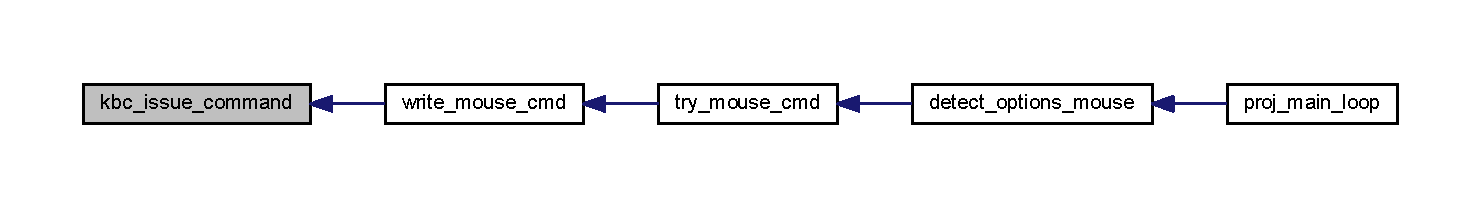
\includegraphics[width=350pt]{group__kbc_ga547e83b3378cd67366e45d3c9565374a_icgraph}
\end{center}
\end{figure}
\mbox{\Hypertarget{group__kbc_ga51a87bc28290c19518e8bbd5423f508a}\label{group__kbc_ga51a87bc28290c19518e8bbd5423f508a}} 
\index{kbc@{kbc}!read\+\_\+information@{read\+\_\+information}}
\index{read\+\_\+information@{read\+\_\+information}!kbc@{kbc}}
\subsubsection{\texorpdfstring{read\+\_\+information()}{read\_information()}}
{\footnotesize\ttfamily int read\+\_\+information (\begin{DoxyParamCaption}\item[{uint8\+\_\+t $\ast$}]{data,  }\item[{uint8\+\_\+t}]{I\+RQ }\end{DoxyParamCaption})}



Reads information of the kbc, whether its the scancode from the keyboard or a packet from the mouse. 


\begin{DoxyParams}{Parameters}
{\em data} & -\/ Pointer to the location where data is stored \\
\hline
{\em I\+RQ} & -\/ I\+RQ line to identify which periphal needs reading \\
\hline
\end{DoxyParams}
\begin{DoxyReturn}{Returns}
int -\/ Returns 0 if successful, returns 1 otherwise 
\end{DoxyReturn}
Here is the caller graph for this function\+:
\nopagebreak
\begin{figure}[H]
\begin{center}
\leavevmode
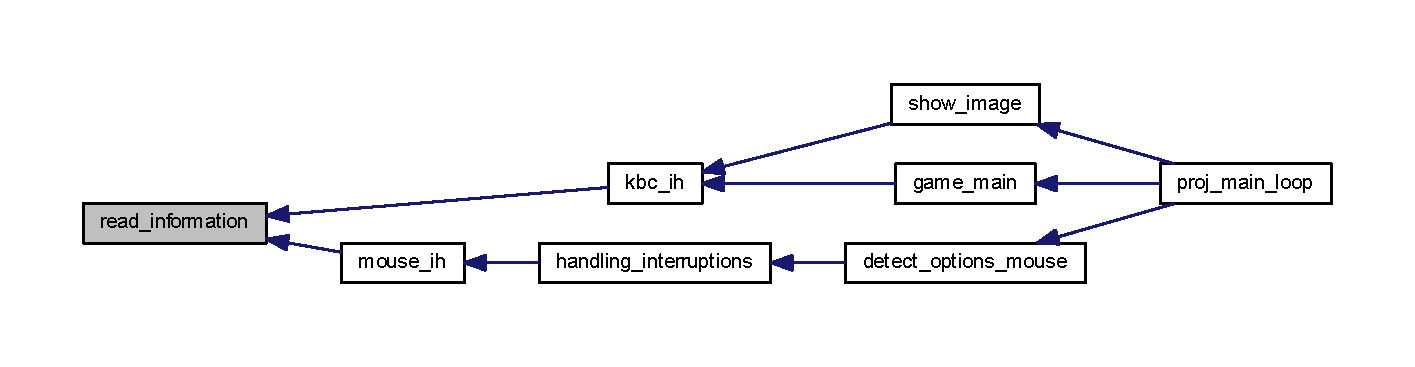
\includegraphics[width=350pt]{group__kbc_ga51a87bc28290c19518e8bbd5423f508a_icgraph}
\end{center}
\end{figure}
\mbox{\Hypertarget{group__kbc_ga77e47edd0806a3ac022baa8431f1f8b8}\label{group__kbc_ga77e47edd0806a3ac022baa8431f1f8b8}} 
\index{kbc@{kbc}!read\+\_\+kbc@{read\+\_\+kbc}}
\index{read\+\_\+kbc@{read\+\_\+kbc}!kbc@{kbc}}
\subsubsection{\texorpdfstring{read\+\_\+kbc()}{read\_kbc()}}
{\footnotesize\ttfamily int read\+\_\+kbc (\begin{DoxyParamCaption}\item[{uint32\+\_\+t $\ast$}]{data,  }\item[{int}]{port }\end{DoxyParamCaption})}



Tries to read information from the kbc status register. 


\begin{DoxyParams}{Parameters}
{\em data} & -\/ Pointer to the location where the data will be stored \\
\hline
{\em port} & -\/ The kbc port to be accessed \\
\hline
\end{DoxyParams}
\begin{DoxyReturn}{Returns}
int -\/ Returns 0 if successful, returns 1 otherwise 
\end{DoxyReturn}
Here is the caller graph for this function\+:
\nopagebreak
\begin{figure}[H]
\begin{center}
\leavevmode
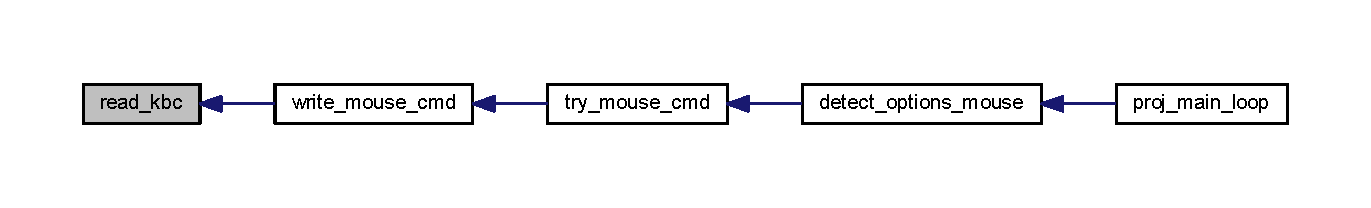
\includegraphics[width=350pt]{group__kbc_ga77e47edd0806a3ac022baa8431f1f8b8_icgraph}
\end{center}
\end{figure}

\hypertarget{group__keyboard}{}\section{keyboard}
\label{group__keyboard}\index{keyboard@{keyboard}}
\subsection*{Functions}
\begin{DoxyCompactItemize}
\item 
int \mbox{\hyperlink{group__keyboard_gaa8e63a9750dae94729779940343f0150}{keyb\+\_\+subscribe\+\_\+int}} (uint8\+\_\+t $\ast$bit\+\_\+no)
\begin{DoxyCompactList}\small\item\em Subscribe keyboard interruptions. \end{DoxyCompactList}\item 
int \mbox{\hyperlink{group__keyboard_gac95aea27a5e91b363b876fed881f368f}{keyboard\+\_\+unsubscribe\+\_\+int}} ()
\begin{DoxyCompactList}\small\item\em Unsubscribe keyboard interruptions. \end{DoxyCompactList}\item 
void \mbox{\hyperlink{group__keyboard_gab9e6ed7960d60aa4834f2038247d4536}{kbc\+\_\+ih}} ()
\begin{DoxyCompactList}\small\item\em 
\begin{DoxyItemize}
\item Keyboard interrupt handler\+: collects information from keyboard 
\end{DoxyItemize}\end{DoxyCompactList}\end{DoxyCompactItemize}


\subsection{Detailed Description}
Functions to handle the keyboard 

\subsection{Function Documentation}
\mbox{\Hypertarget{group__keyboard_gab9e6ed7960d60aa4834f2038247d4536}\label{group__keyboard_gab9e6ed7960d60aa4834f2038247d4536}} 
\index{keyboard@{keyboard}!kbc\+\_\+ih@{kbc\+\_\+ih}}
\index{kbc\+\_\+ih@{kbc\+\_\+ih}!keyboard@{keyboard}}
\subsubsection{\texorpdfstring{kbc\+\_\+ih()}{kbc\_ih()}}
{\footnotesize\ttfamily void kbc\+\_\+ih (\begin{DoxyParamCaption}{ }\end{DoxyParamCaption})}




\begin{DoxyItemize}
\item Keyboard interrupt handler\+: collects information from keyboard 
\end{DoxyItemize}

Here is the call graph for this function\+:
\nopagebreak
\begin{figure}[H]
\begin{center}
\leavevmode
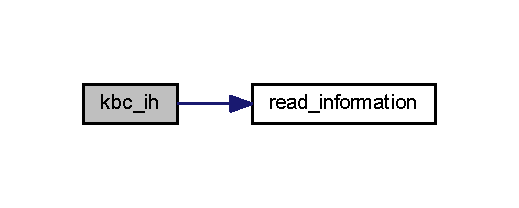
\includegraphics[width=249pt]{group__keyboard_gab9e6ed7960d60aa4834f2038247d4536_cgraph}
\end{center}
\end{figure}
Here is the caller graph for this function\+:
\nopagebreak
\begin{figure}[H]
\begin{center}
\leavevmode
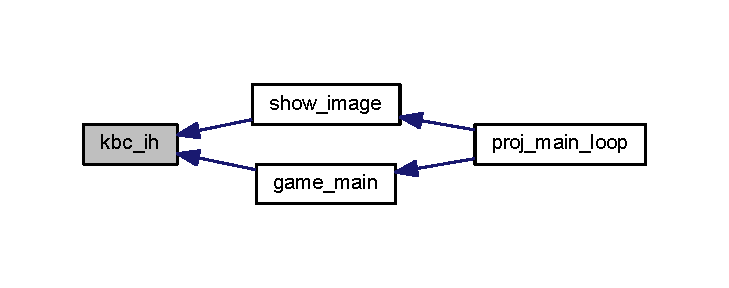
\includegraphics[width=350pt]{group__keyboard_gab9e6ed7960d60aa4834f2038247d4536_icgraph}
\end{center}
\end{figure}
\mbox{\Hypertarget{group__keyboard_gaa8e63a9750dae94729779940343f0150}\label{group__keyboard_gaa8e63a9750dae94729779940343f0150}} 
\index{keyboard@{keyboard}!keyb\+\_\+subscribe\+\_\+int@{keyb\+\_\+subscribe\+\_\+int}}
\index{keyb\+\_\+subscribe\+\_\+int@{keyb\+\_\+subscribe\+\_\+int}!keyboard@{keyboard}}
\subsubsection{\texorpdfstring{keyb\+\_\+subscribe\+\_\+int()}{keyb\_subscribe\_int()}}
{\footnotesize\ttfamily int keyb\+\_\+subscribe\+\_\+int (\begin{DoxyParamCaption}\item[{uint8\+\_\+t $\ast$}]{bit\+\_\+no }\end{DoxyParamCaption})}



Subscribe keyboard interruptions. 


\begin{DoxyParams}{Parameters}
{\em bit\+\_\+no} & -\/ address of memory to be initialized with the bit number to be set in the mask returned upon an interrupt \\
\hline
\end{DoxyParams}
\begin{DoxyReturn}{Returns}
int -\/ Return 0 upon success and non-\/zero otherwise 
\end{DoxyReturn}
Here is the caller graph for this function\+:
\nopagebreak
\begin{figure}[H]
\begin{center}
\leavevmode
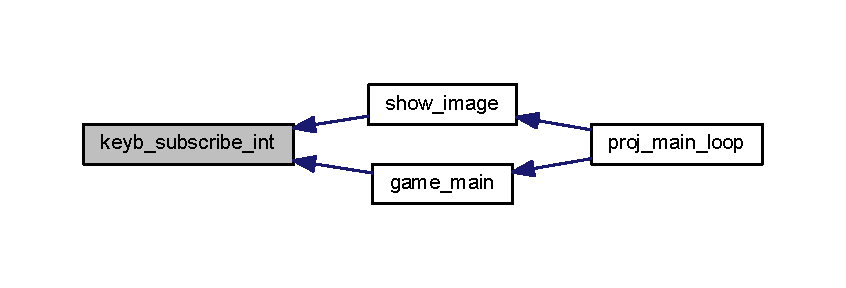
\includegraphics[width=350pt]{group__keyboard_gaa8e63a9750dae94729779940343f0150_icgraph}
\end{center}
\end{figure}
\mbox{\Hypertarget{group__keyboard_gac95aea27a5e91b363b876fed881f368f}\label{group__keyboard_gac95aea27a5e91b363b876fed881f368f}} 
\index{keyboard@{keyboard}!keyboard\+\_\+unsubscribe\+\_\+int@{keyboard\+\_\+unsubscribe\+\_\+int}}
\index{keyboard\+\_\+unsubscribe\+\_\+int@{keyboard\+\_\+unsubscribe\+\_\+int}!keyboard@{keyboard}}
\subsubsection{\texorpdfstring{keyboard\+\_\+unsubscribe\+\_\+int()}{keyboard\_unsubscribe\_int()}}
{\footnotesize\ttfamily int keyboard\+\_\+unsubscribe\+\_\+int (\begin{DoxyParamCaption}{ }\end{DoxyParamCaption})}



Unsubscribe keyboard interruptions. 

\begin{DoxyReturn}{Returns}
int -\/ Return 0 upon success and non-\/zero otherwise 
\end{DoxyReturn}
Here is the caller graph for this function\+:
\nopagebreak
\begin{figure}[H]
\begin{center}
\leavevmode
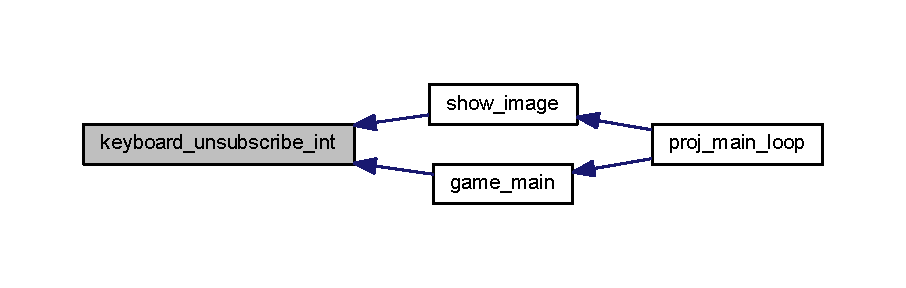
\includegraphics[width=350pt]{group__keyboard_gac95aea27a5e91b363b876fed881f368f_icgraph}
\end{center}
\end{figure}

\hypertarget{group__main__menu}{}\section{main\+\_\+menu}
\label{group__main__menu}\index{main\+\_\+menu@{main\+\_\+menu}}
\subsection*{Data Structures}
\begin{DoxyCompactItemize}
\item 
struct \mbox{\hyperlink{struct_background}{Background}}
\end{DoxyCompactItemize}
\subsection*{Macros}
\begin{DoxyCompactItemize}
\item 
\#define \mbox{\hyperlink{group__main__menu_ga44dd1b46a3f55007e78fc1ac506153b9}{M\+A\+I\+N\+\_\+\+M\+E\+NU}}~0
\item 
\#define \mbox{\hyperlink{group__main__menu_ga81dbe4cce536eb83872b539079ba4139}{G\+A\+ME}}~1
\item 
\#define \mbox{\hyperlink{group__main__menu_ga28017dea6f5becdb38eba6eac6f51bbc}{C\+R\+E\+D\+I\+TS}}~2
\item 
\#define \mbox{\hyperlink{group__main__menu_gad111e603bbebe5d87f6bc39264ce4733}{E\+X\+IT}}~3
\item 
\#define \mbox{\hyperlink{group__main__menu_ga601a4ab83713dad6008bf74c4c347914}{P\+L\+A\+Y\+\_\+X}}~330
\item 
\#define \mbox{\hyperlink{group__main__menu_gab3b9dbde965b2ad8e2b7720c26eded37}{P\+L\+A\+Y\+\_\+\+W\+I\+D\+TH}}~150
\item 
\#define \mbox{\hyperlink{group__main__menu_ga9e84b26e342c1df4348efbfa6694bccd}{P\+L\+A\+Y\+\_\+Y}}~250
\item 
\#define \mbox{\hyperlink{group__main__menu_ga265d0b9390156ec1520c0f68c3431c6c}{P\+L\+A\+Y\+\_\+\+H\+E\+I\+G\+HT}}~45
\item 
\#define \mbox{\hyperlink{group__main__menu_gaeb9fff4c05c42ce4f00cbfe3622b63d0}{C\+R\+E\+D\+I\+T\+S\+\_\+X}}~330
\item 
\#define \mbox{\hyperlink{group__main__menu_gac8aca0d07f517982d67af5081ed2b4f4}{C\+R\+E\+D\+I\+T\+S\+\_\+\+W\+I\+D\+TH}}~150
\item 
\#define \mbox{\hyperlink{group__main__menu_ga2e441d1c4e7d198f1f0d0eb60d331d86}{C\+R\+E\+D\+I\+T\+S\+\_\+Y}}~300
\item 
\#define \mbox{\hyperlink{group__main__menu_gac970a6c034ab2b622434972ef2205935}{C\+R\+E\+D\+I\+T\+S\+\_\+\+H\+E\+I\+G\+HT}}~55
\item 
\#define \mbox{\hyperlink{group__main__menu_ga3040de9a6158b6f62ae7a78d32deffb9}{Q\+U\+I\+T\+\_\+X}}~330
\item 
\#define \mbox{\hyperlink{group__main__menu_ga8e5034a101e70e1f511a56f70f32ad37}{Q\+U\+I\+T\+\_\+\+W\+I\+D\+TH}}~150
\item 
\#define \mbox{\hyperlink{group__main__menu_gae60f4142599ff024b4d8d2ca3ebe42e7}{Q\+U\+I\+T\+\_\+Y}}~380
\item 
\#define \mbox{\hyperlink{group__main__menu_ga3f826023eb74f14d5f48cd11d5385e0a}{Q\+U\+I\+T\+\_\+\+H\+E\+I\+G\+HT}}~45
\item 
\#define \mbox{\hyperlink{group__main__menu_ga5de99031704f5a4356e8fb30d56c4986}{C\+U\+R\+S\+O\+R\+\_\+\+S\+P\+E\+ED}}~1.\+2
\item 
\#define \mbox{\hyperlink{group__main__menu_gae541f04deda5a9c9683f7f3866175023}{C\+U\+R\+S\+O\+R\+\_\+\+S\+I\+ZE}}~20
\end{DoxyCompactItemize}
\subsection*{Functions}
\begin{DoxyCompactItemize}
\item 
int \mbox{\hyperlink{group__main__menu_gae70e892130949697cbf1d294be0adf55}{handling\+\_\+interruptions}} (struct packet $\ast$pp1, uint8\+\_\+t irq\+\_\+set\+\_\+mouse)
\begin{DoxyCompactList}\small\item\em Handles mouse interruptions. \end{DoxyCompactList}\item 
void \mbox{\hyperlink{group__main__menu_ga583b8136014872071b0373049b6fde3c}{draw\+\_\+pointer}} (uint16\+\_\+t x, uint16\+\_\+t y, uint16\+\_\+t color)
\begin{DoxyCompactList}\small\item\em Draw mouse pointer on screen. \end{DoxyCompactList}\item 
int \mbox{\hyperlink{group__main__menu_gadf0b351e14ba0cb60a8d69e8b4423e68}{detect\+\_\+options\+\_\+mouse}} ()
\begin{DoxyCompactList}\small\item\em Tracks the mouse related events, presenting to the user the main menu of the game. \end{DoxyCompactList}\end{DoxyCompactItemize}
\subsection*{Variables}
\begin{DoxyCompactItemize}
\item 
\mbox{\hyperlink{struct_bitmap}{Bitmap}} $\ast$ \mbox{\hyperlink{group__main__menu_ga801bef0ab9d72c95bc5d6d6a0d8f2db0}{image}}
\end{DoxyCompactItemize}


\subsection{Detailed Description}
Functions for handle the main menu events 

\subsection{Macro Definition Documentation}
\mbox{\Hypertarget{group__main__menu_ga28017dea6f5becdb38eba6eac6f51bbc}\label{group__main__menu_ga28017dea6f5becdb38eba6eac6f51bbc}} 
\index{main\+\_\+menu@{main\+\_\+menu}!C\+R\+E\+D\+I\+TS@{C\+R\+E\+D\+I\+TS}}
\index{C\+R\+E\+D\+I\+TS@{C\+R\+E\+D\+I\+TS}!main\+\_\+menu@{main\+\_\+menu}}
\subsubsection{\texorpdfstring{C\+R\+E\+D\+I\+TS}{CREDITS}}
{\footnotesize\ttfamily \#define C\+R\+E\+D\+I\+TS~2}

\mbox{\Hypertarget{group__main__menu_gac970a6c034ab2b622434972ef2205935}\label{group__main__menu_gac970a6c034ab2b622434972ef2205935}} 
\index{main\+\_\+menu@{main\+\_\+menu}!C\+R\+E\+D\+I\+T\+S\+\_\+\+H\+E\+I\+G\+HT@{C\+R\+E\+D\+I\+T\+S\+\_\+\+H\+E\+I\+G\+HT}}
\index{C\+R\+E\+D\+I\+T\+S\+\_\+\+H\+E\+I\+G\+HT@{C\+R\+E\+D\+I\+T\+S\+\_\+\+H\+E\+I\+G\+HT}!main\+\_\+menu@{main\+\_\+menu}}
\subsubsection{\texorpdfstring{C\+R\+E\+D\+I\+T\+S\+\_\+\+H\+E\+I\+G\+HT}{CREDITS\_HEIGHT}}
{\footnotesize\ttfamily \#define C\+R\+E\+D\+I\+T\+S\+\_\+\+H\+E\+I\+G\+HT~55}

\mbox{\Hypertarget{group__main__menu_gac8aca0d07f517982d67af5081ed2b4f4}\label{group__main__menu_gac8aca0d07f517982d67af5081ed2b4f4}} 
\index{main\+\_\+menu@{main\+\_\+menu}!C\+R\+E\+D\+I\+T\+S\+\_\+\+W\+I\+D\+TH@{C\+R\+E\+D\+I\+T\+S\+\_\+\+W\+I\+D\+TH}}
\index{C\+R\+E\+D\+I\+T\+S\+\_\+\+W\+I\+D\+TH@{C\+R\+E\+D\+I\+T\+S\+\_\+\+W\+I\+D\+TH}!main\+\_\+menu@{main\+\_\+menu}}
\subsubsection{\texorpdfstring{C\+R\+E\+D\+I\+T\+S\+\_\+\+W\+I\+D\+TH}{CREDITS\_WIDTH}}
{\footnotesize\ttfamily \#define C\+R\+E\+D\+I\+T\+S\+\_\+\+W\+I\+D\+TH~150}

\mbox{\Hypertarget{group__main__menu_gaeb9fff4c05c42ce4f00cbfe3622b63d0}\label{group__main__menu_gaeb9fff4c05c42ce4f00cbfe3622b63d0}} 
\index{main\+\_\+menu@{main\+\_\+menu}!C\+R\+E\+D\+I\+T\+S\+\_\+X@{C\+R\+E\+D\+I\+T\+S\+\_\+X}}
\index{C\+R\+E\+D\+I\+T\+S\+\_\+X@{C\+R\+E\+D\+I\+T\+S\+\_\+X}!main\+\_\+menu@{main\+\_\+menu}}
\subsubsection{\texorpdfstring{C\+R\+E\+D\+I\+T\+S\+\_\+X}{CREDITS\_X}}
{\footnotesize\ttfamily \#define C\+R\+E\+D\+I\+T\+S\+\_\+X~330}

\mbox{\Hypertarget{group__main__menu_ga2e441d1c4e7d198f1f0d0eb60d331d86}\label{group__main__menu_ga2e441d1c4e7d198f1f0d0eb60d331d86}} 
\index{main\+\_\+menu@{main\+\_\+menu}!C\+R\+E\+D\+I\+T\+S\+\_\+Y@{C\+R\+E\+D\+I\+T\+S\+\_\+Y}}
\index{C\+R\+E\+D\+I\+T\+S\+\_\+Y@{C\+R\+E\+D\+I\+T\+S\+\_\+Y}!main\+\_\+menu@{main\+\_\+menu}}
\subsubsection{\texorpdfstring{C\+R\+E\+D\+I\+T\+S\+\_\+Y}{CREDITS\_Y}}
{\footnotesize\ttfamily \#define C\+R\+E\+D\+I\+T\+S\+\_\+Y~300}

\mbox{\Hypertarget{group__main__menu_gae541f04deda5a9c9683f7f3866175023}\label{group__main__menu_gae541f04deda5a9c9683f7f3866175023}} 
\index{main\+\_\+menu@{main\+\_\+menu}!C\+U\+R\+S\+O\+R\+\_\+\+S\+I\+ZE@{C\+U\+R\+S\+O\+R\+\_\+\+S\+I\+ZE}}
\index{C\+U\+R\+S\+O\+R\+\_\+\+S\+I\+ZE@{C\+U\+R\+S\+O\+R\+\_\+\+S\+I\+ZE}!main\+\_\+menu@{main\+\_\+menu}}
\subsubsection{\texorpdfstring{C\+U\+R\+S\+O\+R\+\_\+\+S\+I\+ZE}{CURSOR\_SIZE}}
{\footnotesize\ttfamily \#define C\+U\+R\+S\+O\+R\+\_\+\+S\+I\+ZE~20}

\mbox{\Hypertarget{group__main__menu_ga5de99031704f5a4356e8fb30d56c4986}\label{group__main__menu_ga5de99031704f5a4356e8fb30d56c4986}} 
\index{main\+\_\+menu@{main\+\_\+menu}!C\+U\+R\+S\+O\+R\+\_\+\+S\+P\+E\+ED@{C\+U\+R\+S\+O\+R\+\_\+\+S\+P\+E\+ED}}
\index{C\+U\+R\+S\+O\+R\+\_\+\+S\+P\+E\+ED@{C\+U\+R\+S\+O\+R\+\_\+\+S\+P\+E\+ED}!main\+\_\+menu@{main\+\_\+menu}}
\subsubsection{\texorpdfstring{C\+U\+R\+S\+O\+R\+\_\+\+S\+P\+E\+ED}{CURSOR\_SPEED}}
{\footnotesize\ttfamily \#define C\+U\+R\+S\+O\+R\+\_\+\+S\+P\+E\+ED~1.\+2}

\mbox{\Hypertarget{group__main__menu_gad111e603bbebe5d87f6bc39264ce4733}\label{group__main__menu_gad111e603bbebe5d87f6bc39264ce4733}} 
\index{main\+\_\+menu@{main\+\_\+menu}!E\+X\+IT@{E\+X\+IT}}
\index{E\+X\+IT@{E\+X\+IT}!main\+\_\+menu@{main\+\_\+menu}}
\subsubsection{\texorpdfstring{E\+X\+IT}{EXIT}}
{\footnotesize\ttfamily \#define E\+X\+IT~3}

\mbox{\Hypertarget{group__main__menu_ga81dbe4cce536eb83872b539079ba4139}\label{group__main__menu_ga81dbe4cce536eb83872b539079ba4139}} 
\index{main\+\_\+menu@{main\+\_\+menu}!G\+A\+ME@{G\+A\+ME}}
\index{G\+A\+ME@{G\+A\+ME}!main\+\_\+menu@{main\+\_\+menu}}
\subsubsection{\texorpdfstring{G\+A\+ME}{GAME}}
{\footnotesize\ttfamily \#define G\+A\+ME~1}

\mbox{\Hypertarget{group__main__menu_ga44dd1b46a3f55007e78fc1ac506153b9}\label{group__main__menu_ga44dd1b46a3f55007e78fc1ac506153b9}} 
\index{main\+\_\+menu@{main\+\_\+menu}!M\+A\+I\+N\+\_\+\+M\+E\+NU@{M\+A\+I\+N\+\_\+\+M\+E\+NU}}
\index{M\+A\+I\+N\+\_\+\+M\+E\+NU@{M\+A\+I\+N\+\_\+\+M\+E\+NU}!main\+\_\+menu@{main\+\_\+menu}}
\subsubsection{\texorpdfstring{M\+A\+I\+N\+\_\+\+M\+E\+NU}{MAIN\_MENU}}
{\footnotesize\ttfamily \#define M\+A\+I\+N\+\_\+\+M\+E\+NU~0}

\mbox{\Hypertarget{group__main__menu_ga265d0b9390156ec1520c0f68c3431c6c}\label{group__main__menu_ga265d0b9390156ec1520c0f68c3431c6c}} 
\index{main\+\_\+menu@{main\+\_\+menu}!P\+L\+A\+Y\+\_\+\+H\+E\+I\+G\+HT@{P\+L\+A\+Y\+\_\+\+H\+E\+I\+G\+HT}}
\index{P\+L\+A\+Y\+\_\+\+H\+E\+I\+G\+HT@{P\+L\+A\+Y\+\_\+\+H\+E\+I\+G\+HT}!main\+\_\+menu@{main\+\_\+menu}}
\subsubsection{\texorpdfstring{P\+L\+A\+Y\+\_\+\+H\+E\+I\+G\+HT}{PLAY\_HEIGHT}}
{\footnotesize\ttfamily \#define P\+L\+A\+Y\+\_\+\+H\+E\+I\+G\+HT~45}

\mbox{\Hypertarget{group__main__menu_gab3b9dbde965b2ad8e2b7720c26eded37}\label{group__main__menu_gab3b9dbde965b2ad8e2b7720c26eded37}} 
\index{main\+\_\+menu@{main\+\_\+menu}!P\+L\+A\+Y\+\_\+\+W\+I\+D\+TH@{P\+L\+A\+Y\+\_\+\+W\+I\+D\+TH}}
\index{P\+L\+A\+Y\+\_\+\+W\+I\+D\+TH@{P\+L\+A\+Y\+\_\+\+W\+I\+D\+TH}!main\+\_\+menu@{main\+\_\+menu}}
\subsubsection{\texorpdfstring{P\+L\+A\+Y\+\_\+\+W\+I\+D\+TH}{PLAY\_WIDTH}}
{\footnotesize\ttfamily \#define P\+L\+A\+Y\+\_\+\+W\+I\+D\+TH~150}

\mbox{\Hypertarget{group__main__menu_ga601a4ab83713dad6008bf74c4c347914}\label{group__main__menu_ga601a4ab83713dad6008bf74c4c347914}} 
\index{main\+\_\+menu@{main\+\_\+menu}!P\+L\+A\+Y\+\_\+X@{P\+L\+A\+Y\+\_\+X}}
\index{P\+L\+A\+Y\+\_\+X@{P\+L\+A\+Y\+\_\+X}!main\+\_\+menu@{main\+\_\+menu}}
\subsubsection{\texorpdfstring{P\+L\+A\+Y\+\_\+X}{PLAY\_X}}
{\footnotesize\ttfamily \#define P\+L\+A\+Y\+\_\+X~330}

\mbox{\Hypertarget{group__main__menu_ga9e84b26e342c1df4348efbfa6694bccd}\label{group__main__menu_ga9e84b26e342c1df4348efbfa6694bccd}} 
\index{main\+\_\+menu@{main\+\_\+menu}!P\+L\+A\+Y\+\_\+Y@{P\+L\+A\+Y\+\_\+Y}}
\index{P\+L\+A\+Y\+\_\+Y@{P\+L\+A\+Y\+\_\+Y}!main\+\_\+menu@{main\+\_\+menu}}
\subsubsection{\texorpdfstring{P\+L\+A\+Y\+\_\+Y}{PLAY\_Y}}
{\footnotesize\ttfamily \#define P\+L\+A\+Y\+\_\+Y~250}

\mbox{\Hypertarget{group__main__menu_ga3f826023eb74f14d5f48cd11d5385e0a}\label{group__main__menu_ga3f826023eb74f14d5f48cd11d5385e0a}} 
\index{main\+\_\+menu@{main\+\_\+menu}!Q\+U\+I\+T\+\_\+\+H\+E\+I\+G\+HT@{Q\+U\+I\+T\+\_\+\+H\+E\+I\+G\+HT}}
\index{Q\+U\+I\+T\+\_\+\+H\+E\+I\+G\+HT@{Q\+U\+I\+T\+\_\+\+H\+E\+I\+G\+HT}!main\+\_\+menu@{main\+\_\+menu}}
\subsubsection{\texorpdfstring{Q\+U\+I\+T\+\_\+\+H\+E\+I\+G\+HT}{QUIT\_HEIGHT}}
{\footnotesize\ttfamily \#define Q\+U\+I\+T\+\_\+\+H\+E\+I\+G\+HT~45}

\mbox{\Hypertarget{group__main__menu_ga8e5034a101e70e1f511a56f70f32ad37}\label{group__main__menu_ga8e5034a101e70e1f511a56f70f32ad37}} 
\index{main\+\_\+menu@{main\+\_\+menu}!Q\+U\+I\+T\+\_\+\+W\+I\+D\+TH@{Q\+U\+I\+T\+\_\+\+W\+I\+D\+TH}}
\index{Q\+U\+I\+T\+\_\+\+W\+I\+D\+TH@{Q\+U\+I\+T\+\_\+\+W\+I\+D\+TH}!main\+\_\+menu@{main\+\_\+menu}}
\subsubsection{\texorpdfstring{Q\+U\+I\+T\+\_\+\+W\+I\+D\+TH}{QUIT\_WIDTH}}
{\footnotesize\ttfamily \#define Q\+U\+I\+T\+\_\+\+W\+I\+D\+TH~150}

\mbox{\Hypertarget{group__main__menu_ga3040de9a6158b6f62ae7a78d32deffb9}\label{group__main__menu_ga3040de9a6158b6f62ae7a78d32deffb9}} 
\index{main\+\_\+menu@{main\+\_\+menu}!Q\+U\+I\+T\+\_\+X@{Q\+U\+I\+T\+\_\+X}}
\index{Q\+U\+I\+T\+\_\+X@{Q\+U\+I\+T\+\_\+X}!main\+\_\+menu@{main\+\_\+menu}}
\subsubsection{\texorpdfstring{Q\+U\+I\+T\+\_\+X}{QUIT\_X}}
{\footnotesize\ttfamily \#define Q\+U\+I\+T\+\_\+X~330}

\mbox{\Hypertarget{group__main__menu_gae60f4142599ff024b4d8d2ca3ebe42e7}\label{group__main__menu_gae60f4142599ff024b4d8d2ca3ebe42e7}} 
\index{main\+\_\+menu@{main\+\_\+menu}!Q\+U\+I\+T\+\_\+Y@{Q\+U\+I\+T\+\_\+Y}}
\index{Q\+U\+I\+T\+\_\+Y@{Q\+U\+I\+T\+\_\+Y}!main\+\_\+menu@{main\+\_\+menu}}
\subsubsection{\texorpdfstring{Q\+U\+I\+T\+\_\+Y}{QUIT\_Y}}
{\footnotesize\ttfamily \#define Q\+U\+I\+T\+\_\+Y~380}



\subsection{Function Documentation}
\mbox{\Hypertarget{group__main__menu_gadf0b351e14ba0cb60a8d69e8b4423e68}\label{group__main__menu_gadf0b351e14ba0cb60a8d69e8b4423e68}} 
\index{main\+\_\+menu@{main\+\_\+menu}!detect\+\_\+options\+\_\+mouse@{detect\+\_\+options\+\_\+mouse}}
\index{detect\+\_\+options\+\_\+mouse@{detect\+\_\+options\+\_\+mouse}!main\+\_\+menu@{main\+\_\+menu}}
\subsubsection{\texorpdfstring{detect\+\_\+options\+\_\+mouse()}{detect\_options\_mouse()}}
{\footnotesize\ttfamily int detect\+\_\+options\+\_\+mouse (\begin{DoxyParamCaption}{ }\end{DoxyParamCaption})}



Tracks the mouse related events, presenting to the user the main menu of the game. 

\begin{DoxyReturn}{Returns}
int -\/ Returns 0 upon sucess and non-\/zero otherwise 
\end{DoxyReturn}
Here is the call graph for this function\+:
\nopagebreak
\begin{figure}[H]
\begin{center}
\leavevmode
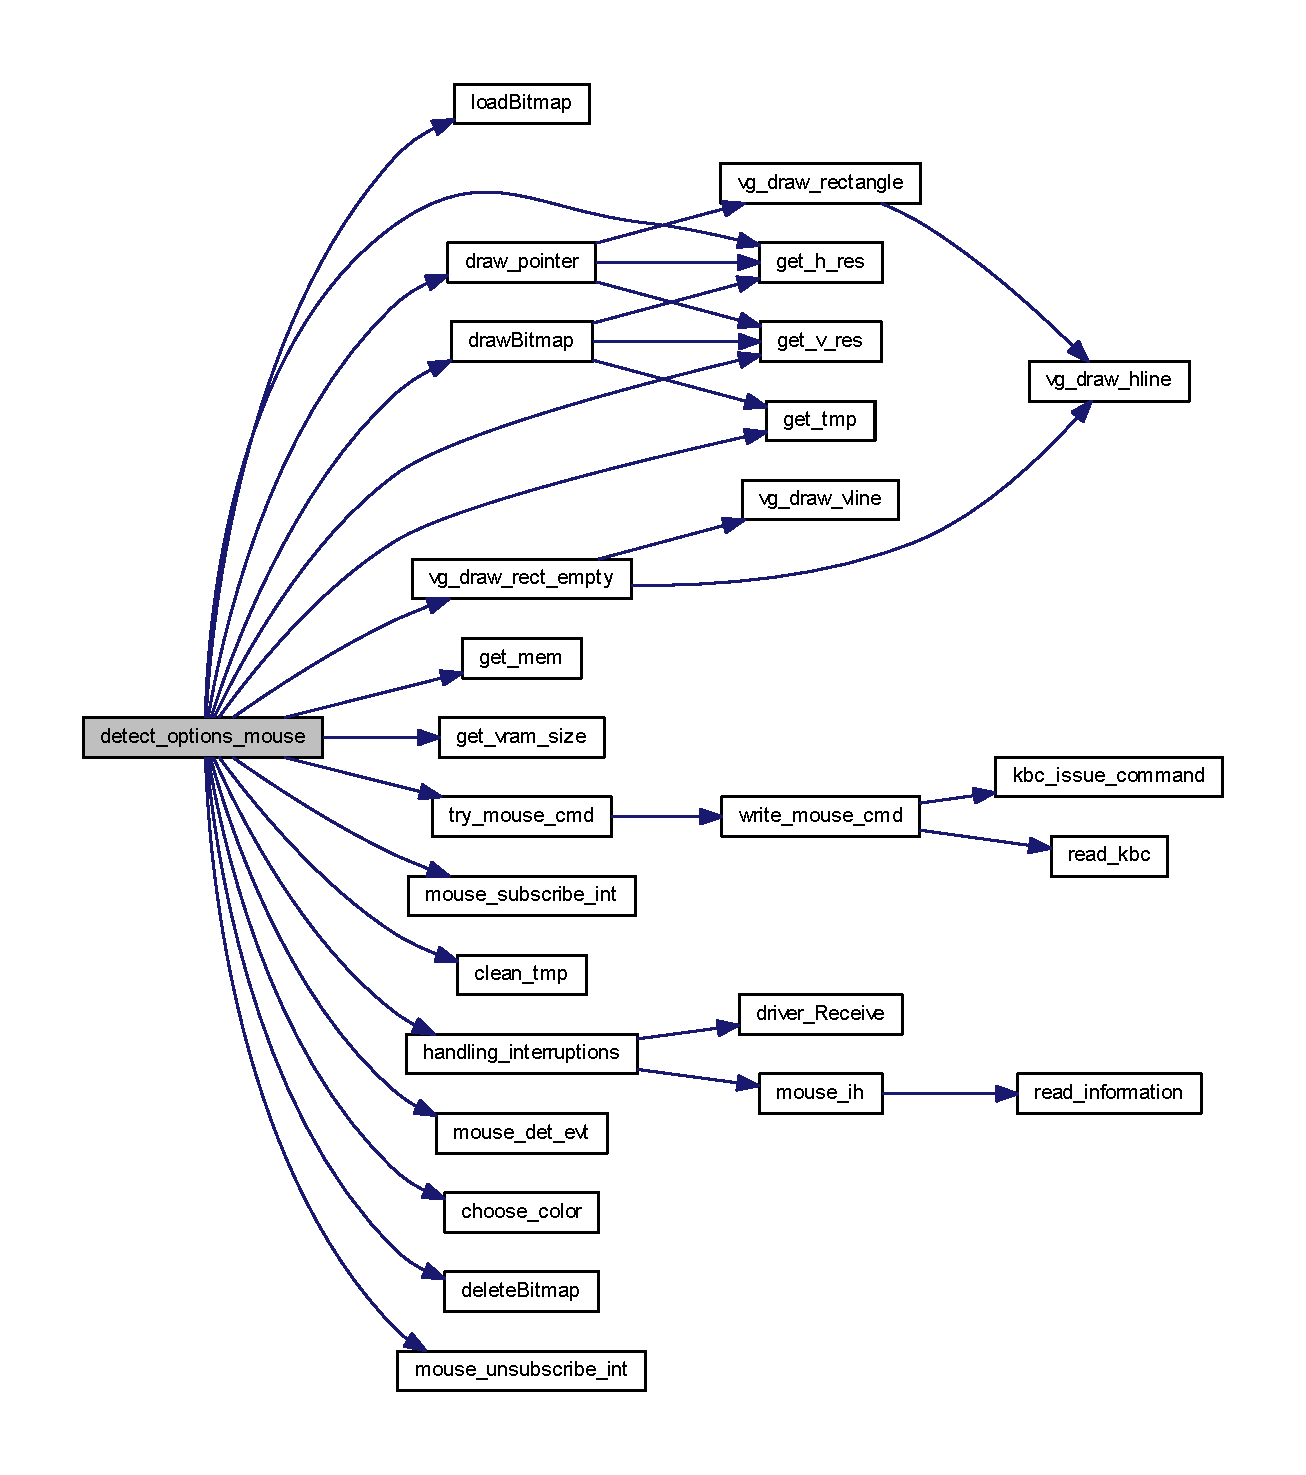
\includegraphics[width=350pt]{group__main__menu_gadf0b351e14ba0cb60a8d69e8b4423e68_cgraph}
\end{center}
\end{figure}
Here is the caller graph for this function\+:
\nopagebreak
\begin{figure}[H]
\begin{center}
\leavevmode
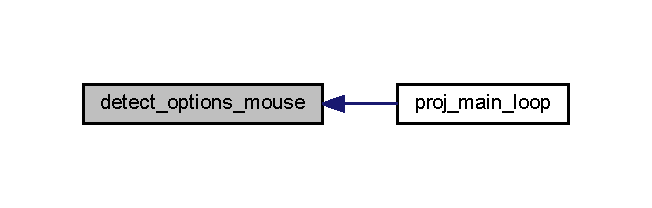
\includegraphics[width=313pt]{group__main__menu_gadf0b351e14ba0cb60a8d69e8b4423e68_icgraph}
\end{center}
\end{figure}
\mbox{\Hypertarget{group__main__menu_ga583b8136014872071b0373049b6fde3c}\label{group__main__menu_ga583b8136014872071b0373049b6fde3c}} 
\index{main\+\_\+menu@{main\+\_\+menu}!draw\+\_\+pointer@{draw\+\_\+pointer}}
\index{draw\+\_\+pointer@{draw\+\_\+pointer}!main\+\_\+menu@{main\+\_\+menu}}
\subsubsection{\texorpdfstring{draw\+\_\+pointer()}{draw\_pointer()}}
{\footnotesize\ttfamily void draw\+\_\+pointer (\begin{DoxyParamCaption}\item[{uint16\+\_\+t}]{x,  }\item[{uint16\+\_\+t}]{y,  }\item[{uint16\+\_\+t}]{color }\end{DoxyParamCaption})}



Draw mouse pointer on screen. 


\begin{DoxyParams}{Parameters}
{\em x} & -\/ horizontal position of mouse on screen \\
\hline
{\em y} & -\/ vertical position of mouse on screen \\
\hline
{\em color} & -\/ color to fill the pointer \\
\hline
\end{DoxyParams}
Here is the call graph for this function\+:
\nopagebreak
\begin{figure}[H]
\begin{center}
\leavevmode
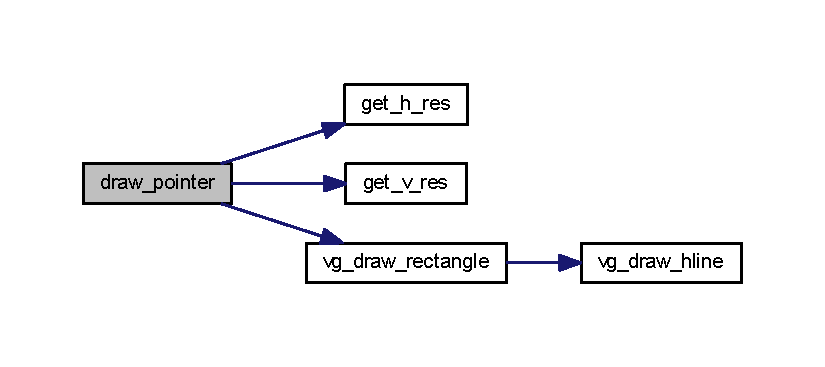
\includegraphics[width=350pt]{group__main__menu_ga583b8136014872071b0373049b6fde3c_cgraph}
\end{center}
\end{figure}
Here is the caller graph for this function\+:
\nopagebreak
\begin{figure}[H]
\begin{center}
\leavevmode
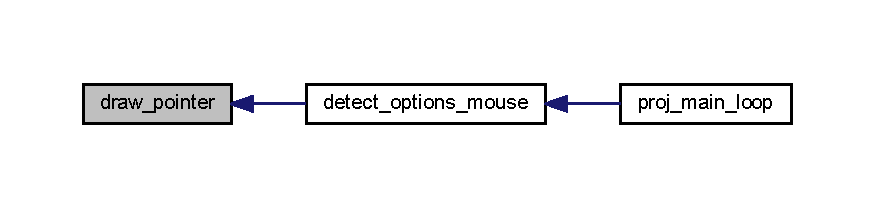
\includegraphics[width=350pt]{group__main__menu_ga583b8136014872071b0373049b6fde3c_icgraph}
\end{center}
\end{figure}
\mbox{\Hypertarget{group__main__menu_gae70e892130949697cbf1d294be0adf55}\label{group__main__menu_gae70e892130949697cbf1d294be0adf55}} 
\index{main\+\_\+menu@{main\+\_\+menu}!handling\+\_\+interruptions@{handling\+\_\+interruptions}}
\index{handling\+\_\+interruptions@{handling\+\_\+interruptions}!main\+\_\+menu@{main\+\_\+menu}}
\subsubsection{\texorpdfstring{handling\+\_\+interruptions()}{handling\_interruptions()}}
{\footnotesize\ttfamily int handling\+\_\+interruptions (\begin{DoxyParamCaption}\item[{struct packet $\ast$}]{pp1,  }\item[{uint8\+\_\+t}]{irq\+\_\+set\+\_\+mouse }\end{DoxyParamCaption})}



Handles mouse interruptions. 


\begin{DoxyParams}{Parameters}
{\em pp1} & -\/ packet of information from mouse \\
\hline
{\em irq\+\_\+set\+\_\+mouse} & -\/ \\
\hline
\end{DoxyParams}
\begin{DoxyReturn}{Returns}
int -\/ Return 0 upon success and non-\/zero otherwise 
\end{DoxyReturn}
Here is the call graph for this function\+:
\nopagebreak
\begin{figure}[H]
\begin{center}
\leavevmode
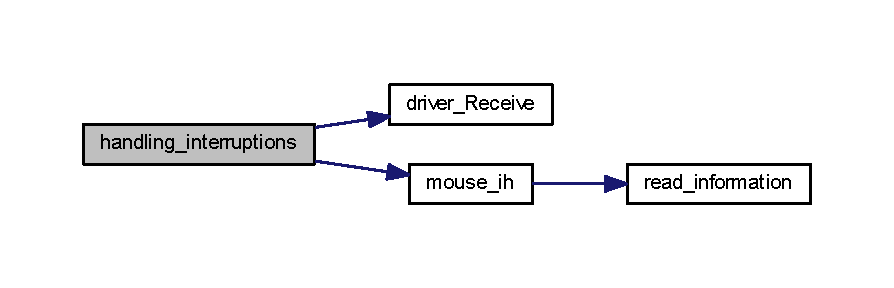
\includegraphics[width=350pt]{group__main__menu_gae70e892130949697cbf1d294be0adf55_cgraph}
\end{center}
\end{figure}
Here is the caller graph for this function\+:
\nopagebreak
\begin{figure}[H]
\begin{center}
\leavevmode
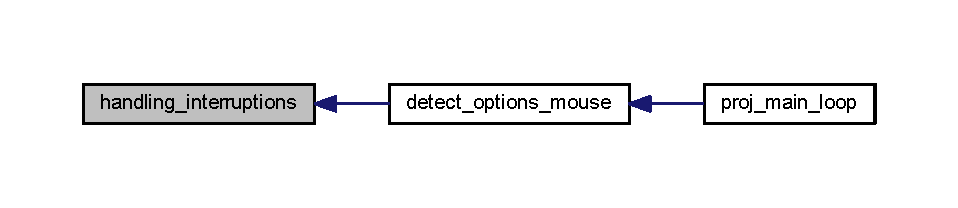
\includegraphics[width=350pt]{group__main__menu_gae70e892130949697cbf1d294be0adf55_icgraph}
\end{center}
\end{figure}


\subsection{Variable Documentation}
\mbox{\Hypertarget{group__main__menu_ga801bef0ab9d72c95bc5d6d6a0d8f2db0}\label{group__main__menu_ga801bef0ab9d72c95bc5d6d6a0d8f2db0}} 
\index{main\+\_\+menu@{main\+\_\+menu}!image@{image}}
\index{image@{image}!main\+\_\+menu@{main\+\_\+menu}}
\subsubsection{\texorpdfstring{image}{image}}
{\footnotesize\ttfamily \mbox{\hyperlink{struct_bitmap}{Bitmap}}$\ast$ image}


\hypertarget{group__mouse}{}\section{mouse}
\label{group__mouse}\index{mouse@{mouse}}
\subsection*{Functions}
\begin{DoxyCompactItemize}
\item 
int \mbox{\hyperlink{group__mouse_ga9da18257ff113b686bb826d154bfaa87}{mouse\+\_\+subscribe\+\_\+int}} (uint8\+\_\+t $\ast$bit\+\_\+no)
\begin{DoxyCompactList}\small\item\em Subscribes mouse interruptions. \end{DoxyCompactList}\item 
int \mbox{\hyperlink{group__mouse_ga685ad2706aca36d9869a30a19b9f446a}{mouse\+\_\+unsubscribe\+\_\+int}} ()
\begin{DoxyCompactList}\small\item\em Unsubscribes mouse interruptions. \end{DoxyCompactList}\item 
int \mbox{\hyperlink{group__mouse_ga992ee1b8a073ba102ee34e483b25c380}{write\+\_\+mouse\+\_\+cmd}} (uint32\+\_\+t mcmd)
\begin{DoxyCompactList}\small\item\em Issues a mouse related command to the keyboard. \end{DoxyCompactList}\item 
int \mbox{\hyperlink{group__mouse_ga34f5d4446d7bc96bd4456ceab5d08ec9}{try\+\_\+mouse\+\_\+cmd}} (uint32\+\_\+t mcmd)
\begin{DoxyCompactList}\small\item\em Tries to issue mouse command while its not successful or an E\+R\+R\+OR byte is received. \end{DoxyCompactList}\item 
void \mbox{\hyperlink{group__mouse_ga834b6d7efe311484d6da234db333cb97}{mouse\+\_\+ih}} ()
\begin{DoxyCompactList}\small\item\em Mouse interrupt handler, reads mouse data from kbc. \end{DoxyCompactList}\item 
struct mouse\+\_\+ev $\ast$ \mbox{\hyperlink{group__mouse_ga992f9c38f09f0aa71b62cba658094dbe}{mouse\+\_\+det\+\_\+evt}} (struct packet $\ast$pp)
\begin{DoxyCompactList}\small\item\em Detects the mouse event by processing the packet passed in the parameter. \end{DoxyCompactList}\end{DoxyCompactItemize}


\subsection{Detailed Description}
Functions for using the P\+S2 mouse 

\subsection{Function Documentation}
\mbox{\Hypertarget{group__mouse_ga992f9c38f09f0aa71b62cba658094dbe}\label{group__mouse_ga992f9c38f09f0aa71b62cba658094dbe}} 
\index{mouse@{mouse}!mouse\+\_\+det\+\_\+evt@{mouse\+\_\+det\+\_\+evt}}
\index{mouse\+\_\+det\+\_\+evt@{mouse\+\_\+det\+\_\+evt}!mouse@{mouse}}
\subsubsection{\texorpdfstring{mouse\+\_\+det\+\_\+evt()}{mouse\_det\_evt()}}
{\footnotesize\ttfamily struct mouse\+\_\+ev$\ast$ mouse\+\_\+det\+\_\+evt (\begin{DoxyParamCaption}\item[{struct packet $\ast$}]{pp }\end{DoxyParamCaption})}



Detects the mouse event by processing the packet passed in the parameter. 


\begin{DoxyParams}{Parameters}
{\em pp} & -\/ Mouse packet to be processed \\
\hline
\end{DoxyParams}
\begin{DoxyReturn}{Returns}
struct mouse\+\_\+ev$\ast$ -\/ Returns a pointer to a struct where the event information is stored 
\end{DoxyReturn}
Here is the caller graph for this function\+:
\nopagebreak
\begin{figure}[H]
\begin{center}
\leavevmode
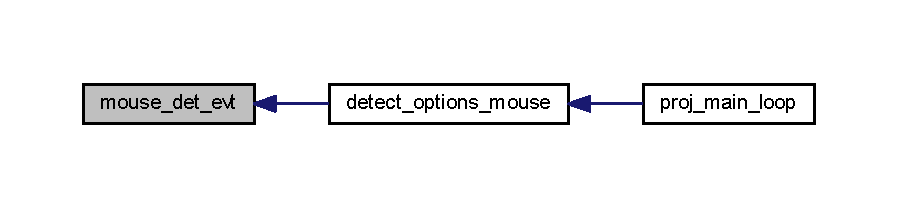
\includegraphics[width=350pt]{group__mouse_ga992f9c38f09f0aa71b62cba658094dbe_icgraph}
\end{center}
\end{figure}
\mbox{\Hypertarget{group__mouse_ga834b6d7efe311484d6da234db333cb97}\label{group__mouse_ga834b6d7efe311484d6da234db333cb97}} 
\index{mouse@{mouse}!mouse\+\_\+ih@{mouse\+\_\+ih}}
\index{mouse\+\_\+ih@{mouse\+\_\+ih}!mouse@{mouse}}
\subsubsection{\texorpdfstring{mouse\+\_\+ih()}{mouse\_ih()}}
{\footnotesize\ttfamily void mouse\+\_\+ih (\begin{DoxyParamCaption}{ }\end{DoxyParamCaption})}



Mouse interrupt handler, reads mouse data from kbc. 

Here is the call graph for this function\+:
\nopagebreak
\begin{figure}[H]
\begin{center}
\leavevmode
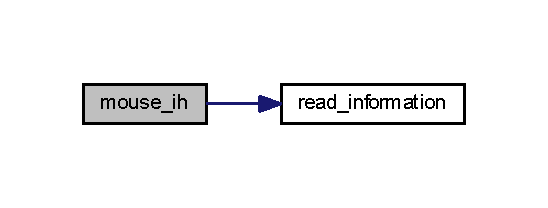
\includegraphics[width=263pt]{group__mouse_ga834b6d7efe311484d6da234db333cb97_cgraph}
\end{center}
\end{figure}
Here is the caller graph for this function\+:
\nopagebreak
\begin{figure}[H]
\begin{center}
\leavevmode
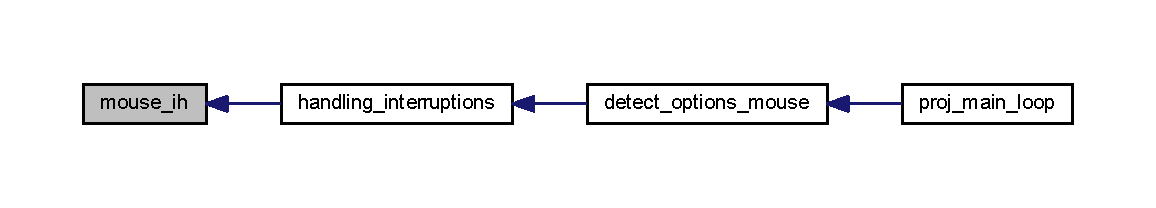
\includegraphics[width=350pt]{group__mouse_ga834b6d7efe311484d6da234db333cb97_icgraph}
\end{center}
\end{figure}
\mbox{\Hypertarget{group__mouse_ga9da18257ff113b686bb826d154bfaa87}\label{group__mouse_ga9da18257ff113b686bb826d154bfaa87}} 
\index{mouse@{mouse}!mouse\+\_\+subscribe\+\_\+int@{mouse\+\_\+subscribe\+\_\+int}}
\index{mouse\+\_\+subscribe\+\_\+int@{mouse\+\_\+subscribe\+\_\+int}!mouse@{mouse}}
\subsubsection{\texorpdfstring{mouse\+\_\+subscribe\+\_\+int()}{mouse\_subscribe\_int()}}
{\footnotesize\ttfamily int mouse\+\_\+subscribe\+\_\+int (\begin{DoxyParamCaption}\item[{uint8\+\_\+t $\ast$}]{bit\+\_\+no }\end{DoxyParamCaption})}



Subscribes mouse interruptions. 


\begin{DoxyParams}{Parameters}
{\em bit\+\_\+no} & -\/ address of memory to be initialized with the bit number to be set in the mask returned upon an interrupt \\
\hline
\end{DoxyParams}
\begin{DoxyReturn}{Returns}
int -\/ Return 0 upon success and non-\/zero otherwise 
\end{DoxyReturn}
Here is the caller graph for this function\+:
\nopagebreak
\begin{figure}[H]
\begin{center}
\leavevmode
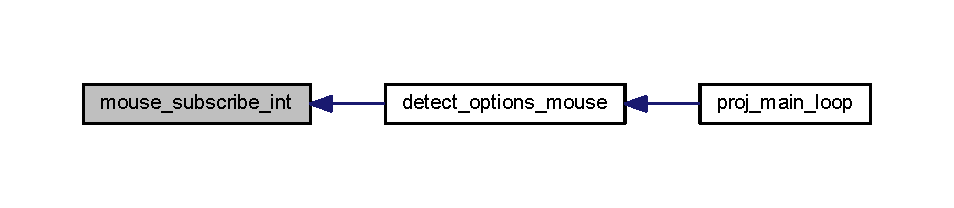
\includegraphics[width=350pt]{group__mouse_ga9da18257ff113b686bb826d154bfaa87_icgraph}
\end{center}
\end{figure}
\mbox{\Hypertarget{group__mouse_ga685ad2706aca36d9869a30a19b9f446a}\label{group__mouse_ga685ad2706aca36d9869a30a19b9f446a}} 
\index{mouse@{mouse}!mouse\+\_\+unsubscribe\+\_\+int@{mouse\+\_\+unsubscribe\+\_\+int}}
\index{mouse\+\_\+unsubscribe\+\_\+int@{mouse\+\_\+unsubscribe\+\_\+int}!mouse@{mouse}}
\subsubsection{\texorpdfstring{mouse\+\_\+unsubscribe\+\_\+int()}{mouse\_unsubscribe\_int()}}
{\footnotesize\ttfamily int mouse\+\_\+unsubscribe\+\_\+int (\begin{DoxyParamCaption}{ }\end{DoxyParamCaption})}



Unsubscribes mouse interruptions. 

\begin{DoxyReturn}{Returns}
int -\/ Return 0 upon success and non-\/zero otherwise 
\end{DoxyReturn}
Here is the caller graph for this function\+:
\nopagebreak
\begin{figure}[H]
\begin{center}
\leavevmode
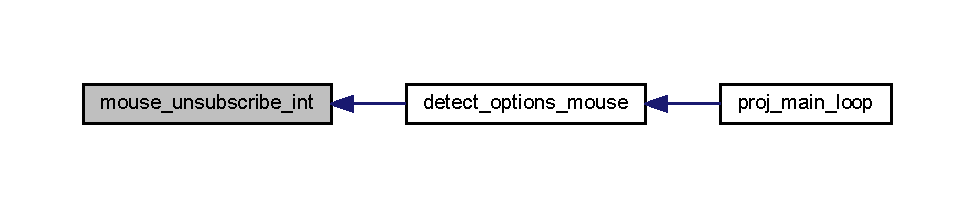
\includegraphics[width=350pt]{group__mouse_ga685ad2706aca36d9869a30a19b9f446a_icgraph}
\end{center}
\end{figure}
\mbox{\Hypertarget{group__mouse_ga34f5d4446d7bc96bd4456ceab5d08ec9}\label{group__mouse_ga34f5d4446d7bc96bd4456ceab5d08ec9}} 
\index{mouse@{mouse}!try\+\_\+mouse\+\_\+cmd@{try\+\_\+mouse\+\_\+cmd}}
\index{try\+\_\+mouse\+\_\+cmd@{try\+\_\+mouse\+\_\+cmd}!mouse@{mouse}}
\subsubsection{\texorpdfstring{try\+\_\+mouse\+\_\+cmd()}{try\_mouse\_cmd()}}
{\footnotesize\ttfamily int try\+\_\+mouse\+\_\+cmd (\begin{DoxyParamCaption}\item[{uint32\+\_\+t}]{mcmd }\end{DoxyParamCaption})}



Tries to issue mouse command while its not successful or an E\+R\+R\+OR byte is received. 


\begin{DoxyParams}{Parameters}
{\em mcmd} & -\/ Command to be issued \\
\hline
\end{DoxyParams}
\begin{DoxyReturn}{Returns}
int -\/ Return 0 upon success and non-\/zero otherwise 
\end{DoxyReturn}
Here is the call graph for this function\+:
\nopagebreak
\begin{figure}[H]
\begin{center}
\leavevmode
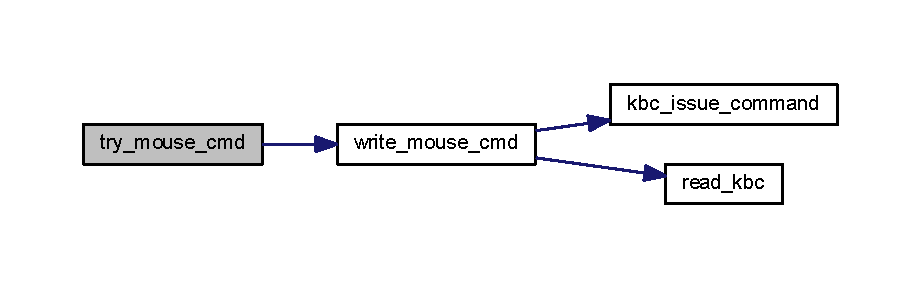
\includegraphics[width=350pt]{group__mouse_ga34f5d4446d7bc96bd4456ceab5d08ec9_cgraph}
\end{center}
\end{figure}
Here is the caller graph for this function\+:
\nopagebreak
\begin{figure}[H]
\begin{center}
\leavevmode
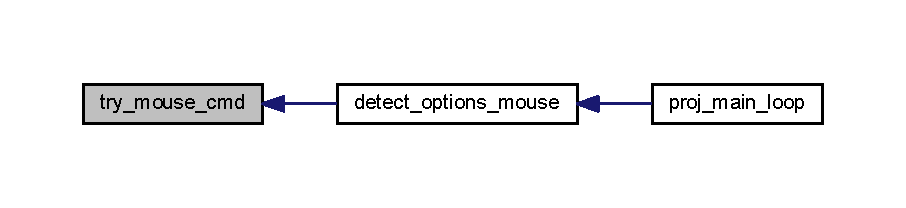
\includegraphics[width=350pt]{group__mouse_ga34f5d4446d7bc96bd4456ceab5d08ec9_icgraph}
\end{center}
\end{figure}
\mbox{\Hypertarget{group__mouse_ga992ee1b8a073ba102ee34e483b25c380}\label{group__mouse_ga992ee1b8a073ba102ee34e483b25c380}} 
\index{mouse@{mouse}!write\+\_\+mouse\+\_\+cmd@{write\+\_\+mouse\+\_\+cmd}}
\index{write\+\_\+mouse\+\_\+cmd@{write\+\_\+mouse\+\_\+cmd}!mouse@{mouse}}
\subsubsection{\texorpdfstring{write\+\_\+mouse\+\_\+cmd()}{write\_mouse\_cmd()}}
{\footnotesize\ttfamily int write\+\_\+mouse\+\_\+cmd (\begin{DoxyParamCaption}\item[{uint32\+\_\+t}]{mcmd }\end{DoxyParamCaption})}



Issues a mouse related command to the keyboard. 


\begin{DoxyParams}{Parameters}
{\em mcmd} & -\/ Command to be issued \\
\hline
\end{DoxyParams}
\begin{DoxyReturn}{Returns}
int -\/ Return 0 if A\+CK byte is received, 1 if N\+A\+CK byte is received and 2 if E\+R\+R\+OR byte is received. 
\end{DoxyReturn}
Here is the call graph for this function\+:
\nopagebreak
\begin{figure}[H]
\begin{center}
\leavevmode
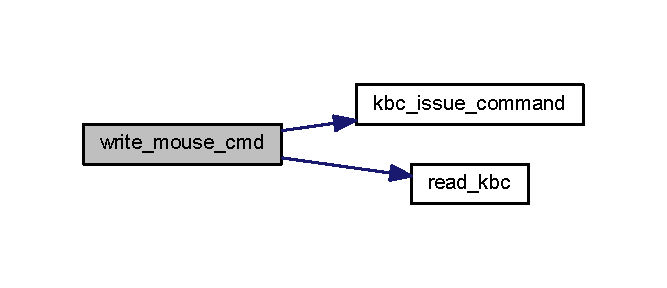
\includegraphics[width=320pt]{group__mouse_ga992ee1b8a073ba102ee34e483b25c380_cgraph}
\end{center}
\end{figure}
Here is the caller graph for this function\+:
\nopagebreak
\begin{figure}[H]
\begin{center}
\leavevmode
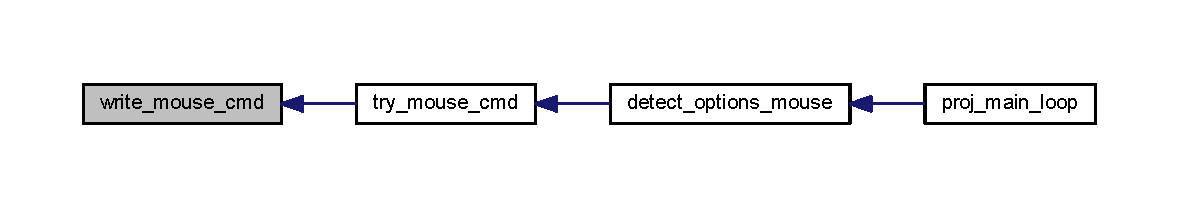
\includegraphics[width=350pt]{group__mouse_ga992ee1b8a073ba102ee34e483b25c380_icgraph}
\end{center}
\end{figure}

\hypertarget{group__rtc}{}\section{rtc}
\label{group__rtc}\index{rtc@{rtc}}
\subsection*{Data Structures}
\begin{DoxyCompactItemize}
\item 
struct \mbox{\hyperlink{struct_date}{Date}}
\end{DoxyCompactItemize}
\subsection*{Macros}
\begin{DoxyCompactItemize}
\item 
\#define \mbox{\hyperlink{group__rtc_gad27cc17b25bb93134368d5eb21126eae}{B\+IT}}(x)~1$<$$<$x
\item 
\#define \mbox{\hyperlink{group__rtc_ga4e22feb6ffbc1cda32fadff5c740dc51}{R\+T\+C\+\_\+\+I\+RQ}}~8
\item 
\#define \mbox{\hyperlink{group__rtc_gaee714b0468cb683740ae28b1e0ad25e6}{A\+D\+D\+R\+\_\+\+R\+EG}}~0x70
\item 
\#define \mbox{\hyperlink{group__rtc_ga71b8ba376f687142f60a82d18c2715e0}{D\+A\+T\+A\+\_\+\+R\+EG}}~0x71
\item 
\#define \mbox{\hyperlink{group__rtc_ga48fcf4f2eeef6769d588168d4ac2ab0e}{S\+E\+C\+O\+N\+DS}}~0x00
\item 
\#define \mbox{\hyperlink{group__rtc_ga84be9dcfa5a172ee83121620d15c8e29}{M\+I\+N\+U\+T\+ES}}~0x02
\item 
\#define \mbox{\hyperlink{group__rtc_ga212d0f839f6f7ca43ccde311f93d5892}{H\+O\+U\+RS}}~0x04
\item 
\#define \mbox{\hyperlink{group__rtc_gacd522b0e92d01c9bb65527206fc17508}{D\+A\+Y\+\_\+\+W\+E\+EK}}~0x06
\item 
\#define \mbox{\hyperlink{group__rtc_gaa652d6d52e8e86bfd3659f873c87a340}{D\+A\+Y\+\_\+\+M\+O\+N\+TH}}~0x07
\item 
\#define \mbox{\hyperlink{group__rtc_ga3729d06495d9713592f79f3122c9e677}{M\+O\+N\+TH}}~0x08
\item 
\#define \mbox{\hyperlink{group__rtc_ga5871356500f559add06ea81d60331b1b}{Y\+E\+AR}}~0x09
\item 
\#define \mbox{\hyperlink{group__rtc_gaa0e40d1cb9fea79e800aa79b8ca291f7}{R\+E\+G\+\_\+A}}~0x0A
\item 
\#define \mbox{\hyperlink{group__rtc_ga28ed75c6727784e56c2bb8d828c876c9}{R\+E\+G\+\_\+B}}~0x0B
\item 
\#define \mbox{\hyperlink{group__rtc_ga088e580de0961d5f30eb3366f97b324c}{R\+E\+G\+\_\+C}}~0x0C
\item 
\#define \mbox{\hyperlink{group__rtc_ga8f2a2da8b96e20112d3f225636392424}{R\+E\+G\+\_\+D}}~0\+X0D
\item 
\#define \mbox{\hyperlink{group__rtc_ga3289eebd69837790d4aacaccd18d46db}{U\+IP}}~\mbox{\hyperlink{group__vbe_ga3a8ea58898cb58fc96013383d39f482c}{B\+IT}}(7)
\item 
\#define \mbox{\hyperlink{group__rtc_ga7ebe68dabb3864696a8a466499fbc37d}{S\+E\+T\+\_\+\+R\+TC}}~\mbox{\hyperlink{group__vbe_ga3a8ea58898cb58fc96013383d39f482c}{B\+IT}}(7)
\item 
\#define \mbox{\hyperlink{group__rtc_gac40c2b49eb51e2adc237b530adfcadf4}{P\+IE}}~\mbox{\hyperlink{group__vbe_ga3a8ea58898cb58fc96013383d39f482c}{B\+IT}}(6)
\item 
\#define \mbox{\hyperlink{group__rtc_ga113847820d539c6a6836993b84d22800}{A\+IE}}~\mbox{\hyperlink{group__vbe_ga3a8ea58898cb58fc96013383d39f482c}{B\+IT}}(5)
\item 
\#define \mbox{\hyperlink{group__rtc_ga2c276876faf62c1b29fe2383ce4ccfda}{U\+IE}}~\mbox{\hyperlink{group__vbe_ga3a8ea58898cb58fc96013383d39f482c}{B\+IT}}(4)
\item 
\#define \mbox{\hyperlink{group__rtc_ga96df1c1afaaa70a1b805c83bad18ff26}{B\+I\+N\+A\+R\+Y\+\_\+\+DM}}~\mbox{\hyperlink{group__vbe_ga3a8ea58898cb58fc96013383d39f482c}{B\+IT}}(2)
\item 
\#define \mbox{\hyperlink{group__rtc_ga70514fa1fe27f2ca52b651ff16ed0069}{T\+I\+M\+E\+\_\+\+F\+O\+R\+M\+A\+T\+\_\+24H}}~\mbox{\hyperlink{group__vbe_ga3a8ea58898cb58fc96013383d39f482c}{B\+IT}}(1)
\item 
\#define \mbox{\hyperlink{group__rtc_ga8565773f11252b9d615f1b12ac73032d}{I\+R\+QF}}~\mbox{\hyperlink{group__vbe_ga3a8ea58898cb58fc96013383d39f482c}{B\+IT}}(7)
\item 
\#define \mbox{\hyperlink{group__rtc_gaa0e278c26c25558741febfadd7216caa}{PF}}~\mbox{\hyperlink{group__vbe_ga3a8ea58898cb58fc96013383d39f482c}{B\+IT}}(6)
\item 
\#define \mbox{\hyperlink{group__rtc_ga76ba789cde9c36cd57dbb390bdee7661}{AF}}~\mbox{\hyperlink{group__vbe_ga3a8ea58898cb58fc96013383d39f482c}{B\+IT}}(5)
\item 
\#define \mbox{\hyperlink{group__rtc_ga2657a76f02e47fa3f3320fa9c6353f31}{UF}}~\mbox{\hyperlink{group__vbe_ga3a8ea58898cb58fc96013383d39f482c}{B\+IT}}(4)
\end{DoxyCompactItemize}
\subsection*{Functions}
\begin{DoxyCompactItemize}
\item 
int \mbox{\hyperlink{group__rtc_ga7c28e3528db0f743706f9c01608331a7}{rtc\+\_\+subscribe\+\_\+int}} (uint8\+\_\+t $\ast$bitno)
\begin{DoxyCompactList}\small\item\em Subscribes R\+TC interruptions. \end{DoxyCompactList}\item 
int \mbox{\hyperlink{group__rtc_gab8f17bf5280c908c8b199a90fefcc758}{rtc\+\_\+unsubscribe\+\_\+int}} ()
\begin{DoxyCompactList}\small\item\em Unsubscribes R\+TC interruptions. \end{DoxyCompactList}\item 
int \mbox{\hyperlink{group__rtc_gaf6f18245f611a9c8f64055feae5ec73d}{rtc\+\_\+read\+\_\+register}} (uint32\+\_\+t addr, uint32\+\_\+t $\ast$\mbox{\hyperlink{mouse_8c_a325819a8e492ac69542e8b31705af6e9}{data}})
\begin{DoxyCompactList}\small\item\em Reads R\+TC address passed in the arguments and stores it. \end{DoxyCompactList}\item 
int \mbox{\hyperlink{group__rtc_ga9b5d85527d676067a8c05780ec46d4f1}{rtc\+\_\+write\+\_\+register}} (uint32\+\_\+t addr, uint32\+\_\+t \mbox{\hyperlink{mouse_8c_a325819a8e492ac69542e8b31705af6e9}{data}})
\begin{DoxyCompactList}\small\item\em Writes to the R\+TC address passed in the arguments. \end{DoxyCompactList}\item 
int \mbox{\hyperlink{group__rtc_ga33036209deeaa3ca32027fdab0c8b2d7}{rtc\+\_\+enable\+\_\+update\+\_\+ints}} ()
\begin{DoxyCompactList}\small\item\em Enables update-\/ended interruptions. \end{DoxyCompactList}\item 
int \mbox{\hyperlink{group__rtc_ga6222d2da81f961f574c428db117e610e}{rtc\+\_\+disable\+\_\+update\+\_\+ints}} ()
\begin{DoxyCompactList}\small\item\em Disables update-\/ended interruptions. \end{DoxyCompactList}\item 
uint32\+\_\+t \mbox{\hyperlink{group__rtc_ga3d9330b99a772073f924e69bc1b2df05}{rtc\+\_\+read\+\_\+seconds}} ()
\begin{DoxyCompactList}\small\item\em Reads seconds from the appropriate register. \end{DoxyCompactList}\item 
uint32\+\_\+t \mbox{\hyperlink{group__rtc_gaac43b2266aa06ad5a572d0fa3976ebb0}{rtc\+\_\+read\+\_\+minutes}} ()
\begin{DoxyCompactList}\small\item\em Reads minutes from the appropriate register. \end{DoxyCompactList}\item 
uint32\+\_\+t \mbox{\hyperlink{group__rtc_ga512adcbde067ca5bb83b1af0e0a7a444}{rtc\+\_\+read\+\_\+hours}} ()
\begin{DoxyCompactList}\small\item\em Reads hour from the appropriate register. \end{DoxyCompactList}\item 
uint32\+\_\+t \mbox{\hyperlink{group__rtc_ga2e585f34d69246a60a1db0e94ca09c05}{rtc\+\_\+read\+\_\+day\+\_\+week}} ()
\begin{DoxyCompactList}\small\item\em Reads day of the week from the appropriate register. \end{DoxyCompactList}\item 
uint32\+\_\+t \mbox{\hyperlink{group__rtc_ga59359f9460af7b7dce7a2c8dc9d98211}{rtc\+\_\+read\+\_\+day\+\_\+month}} ()
\begin{DoxyCompactList}\small\item\em Reads day of the month from the appropriate register. \end{DoxyCompactList}\item 
uint32\+\_\+t \mbox{\hyperlink{group__rtc_gabd90445bf474121fa89636a17f4c7369}{rtc\+\_\+read\+\_\+month}} ()
\begin{DoxyCompactList}\small\item\em Reads month from the appropriate register. \end{DoxyCompactList}\item 
uint32\+\_\+t \mbox{\hyperlink{group__rtc_ga4ddd82a19df760d95b2dd0c92ec6c63b}{rtc\+\_\+read\+\_\+year}} ()
\begin{DoxyCompactList}\small\item\em Reads year from the appropriate register. \end{DoxyCompactList}\item 
void \mbox{\hyperlink{group__rtc_ga75dad42881d64cf07cf1bdc2979a7056}{rtc\+\_\+ih}} ()
\begin{DoxyCompactList}\small\item\em R\+TC interrupt handler, reads register C to verify what is the source of the interruptions and handles the information accordingly. \end{DoxyCompactList}\item 
\mbox{\hyperlink{struct_date}{Date}} \mbox{\hyperlink{group__rtc_ga1f2c4f317d879fe00426ee4317bc625f}{get\+\_\+date}} ()
\begin{DoxyCompactList}\small\item\em Get the \mbox{\hyperlink{struct_date}{Date}} object. \end{DoxyCompactList}\item 
int \mbox{\hyperlink{group__rtc_ga1c7900b102529826ac1662355e6cf058}{rtc\+\_\+update\+\_\+date}} ()
\begin{DoxyCompactList}\small\item\em Update the \mbox{\hyperlink{struct_date}{Date}} object with new information. \end{DoxyCompactList}\end{DoxyCompactItemize}
\subsection*{Variables}
\begin{DoxyCompactItemize}
\item 
uint32\+\_\+t \mbox{\hyperlink{group__rtc_gaac3a162d2f192fe2360aba534eac7198}{year}}
\item 
uint32\+\_\+t \mbox{\hyperlink{group__rtc_ga55a5fa57878363d803833666ddf3c16f}{month}}
\item 
uint32\+\_\+t \mbox{\hyperlink{group__rtc_ga897ed87b95b7a37afeeb935ca0b2366b}{day}}
\item 
uint32\+\_\+t \mbox{\hyperlink{group__rtc_gaa24f12f79f7553236083be08521c546e}{dayW}}
\item 
uint32\+\_\+t \mbox{\hyperlink{group__rtc_ga26d5bae76d83086900174b266fd2cd82}{hour}}
\item 
uint32\+\_\+t \mbox{\hyperlink{group__rtc_ga2dcb690348d97b756f4d165c80c9af7d}{minutes}}
\item 
uint32\+\_\+t \mbox{\hyperlink{group__rtc_ga6d5694839ec935781627e5c52de21fda}{seconds}}
\end{DoxyCompactItemize}


\subsection{Detailed Description}
Functions for using the real-\/time clock 

\subsection{Macro Definition Documentation}
\mbox{\Hypertarget{group__rtc_gaee714b0468cb683740ae28b1e0ad25e6}\label{group__rtc_gaee714b0468cb683740ae28b1e0ad25e6}} 
\index{rtc@{rtc}!A\+D\+D\+R\+\_\+\+R\+EG@{A\+D\+D\+R\+\_\+\+R\+EG}}
\index{A\+D\+D\+R\+\_\+\+R\+EG@{A\+D\+D\+R\+\_\+\+R\+EG}!rtc@{rtc}}
\subsubsection{\texorpdfstring{A\+D\+D\+R\+\_\+\+R\+EG}{ADDR\_REG}}
{\footnotesize\ttfamily \#define A\+D\+D\+R\+\_\+\+R\+EG~0x70}

\mbox{\Hypertarget{group__rtc_ga76ba789cde9c36cd57dbb390bdee7661}\label{group__rtc_ga76ba789cde9c36cd57dbb390bdee7661}} 
\index{rtc@{rtc}!AF@{AF}}
\index{AF@{AF}!rtc@{rtc}}
\subsubsection{\texorpdfstring{AF}{AF}}
{\footnotesize\ttfamily \#define AF~\mbox{\hyperlink{group__vbe_ga3a8ea58898cb58fc96013383d39f482c}{B\+IT}}(5)}

\mbox{\Hypertarget{group__rtc_ga113847820d539c6a6836993b84d22800}\label{group__rtc_ga113847820d539c6a6836993b84d22800}} 
\index{rtc@{rtc}!A\+IE@{A\+IE}}
\index{A\+IE@{A\+IE}!rtc@{rtc}}
\subsubsection{\texorpdfstring{A\+IE}{AIE}}
{\footnotesize\ttfamily \#define A\+IE~\mbox{\hyperlink{group__vbe_ga3a8ea58898cb58fc96013383d39f482c}{B\+IT}}(5)}

\mbox{\Hypertarget{group__rtc_ga96df1c1afaaa70a1b805c83bad18ff26}\label{group__rtc_ga96df1c1afaaa70a1b805c83bad18ff26}} 
\index{rtc@{rtc}!B\+I\+N\+A\+R\+Y\+\_\+\+DM@{B\+I\+N\+A\+R\+Y\+\_\+\+DM}}
\index{B\+I\+N\+A\+R\+Y\+\_\+\+DM@{B\+I\+N\+A\+R\+Y\+\_\+\+DM}!rtc@{rtc}}
\subsubsection{\texorpdfstring{B\+I\+N\+A\+R\+Y\+\_\+\+DM}{BINARY\_DM}}
{\footnotesize\ttfamily \#define B\+I\+N\+A\+R\+Y\+\_\+\+DM~\mbox{\hyperlink{group__vbe_ga3a8ea58898cb58fc96013383d39f482c}{B\+IT}}(2)}

\mbox{\Hypertarget{group__rtc_gad27cc17b25bb93134368d5eb21126eae}\label{group__rtc_gad27cc17b25bb93134368d5eb21126eae}} 
\index{rtc@{rtc}!B\+IT@{B\+IT}}
\index{B\+IT@{B\+IT}!rtc@{rtc}}
\subsubsection{\texorpdfstring{B\+IT}{BIT}}
{\footnotesize\ttfamily \#define B\+IT(\begin{DoxyParamCaption}\item[{}]{x }\end{DoxyParamCaption})~1$<$$<$x}

\mbox{\Hypertarget{group__rtc_ga71b8ba376f687142f60a82d18c2715e0}\label{group__rtc_ga71b8ba376f687142f60a82d18c2715e0}} 
\index{rtc@{rtc}!D\+A\+T\+A\+\_\+\+R\+EG@{D\+A\+T\+A\+\_\+\+R\+EG}}
\index{D\+A\+T\+A\+\_\+\+R\+EG@{D\+A\+T\+A\+\_\+\+R\+EG}!rtc@{rtc}}
\subsubsection{\texorpdfstring{D\+A\+T\+A\+\_\+\+R\+EG}{DATA\_REG}}
{\footnotesize\ttfamily \#define D\+A\+T\+A\+\_\+\+R\+EG~0x71}

\mbox{\Hypertarget{group__rtc_gaa652d6d52e8e86bfd3659f873c87a340}\label{group__rtc_gaa652d6d52e8e86bfd3659f873c87a340}} 
\index{rtc@{rtc}!D\+A\+Y\+\_\+\+M\+O\+N\+TH@{D\+A\+Y\+\_\+\+M\+O\+N\+TH}}
\index{D\+A\+Y\+\_\+\+M\+O\+N\+TH@{D\+A\+Y\+\_\+\+M\+O\+N\+TH}!rtc@{rtc}}
\subsubsection{\texorpdfstring{D\+A\+Y\+\_\+\+M\+O\+N\+TH}{DAY\_MONTH}}
{\footnotesize\ttfamily \#define D\+A\+Y\+\_\+\+M\+O\+N\+TH~0x07}

\mbox{\Hypertarget{group__rtc_gacd522b0e92d01c9bb65527206fc17508}\label{group__rtc_gacd522b0e92d01c9bb65527206fc17508}} 
\index{rtc@{rtc}!D\+A\+Y\+\_\+\+W\+E\+EK@{D\+A\+Y\+\_\+\+W\+E\+EK}}
\index{D\+A\+Y\+\_\+\+W\+E\+EK@{D\+A\+Y\+\_\+\+W\+E\+EK}!rtc@{rtc}}
\subsubsection{\texorpdfstring{D\+A\+Y\+\_\+\+W\+E\+EK}{DAY\_WEEK}}
{\footnotesize\ttfamily \#define D\+A\+Y\+\_\+\+W\+E\+EK~0x06}

\mbox{\Hypertarget{group__rtc_ga212d0f839f6f7ca43ccde311f93d5892}\label{group__rtc_ga212d0f839f6f7ca43ccde311f93d5892}} 
\index{rtc@{rtc}!H\+O\+U\+RS@{H\+O\+U\+RS}}
\index{H\+O\+U\+RS@{H\+O\+U\+RS}!rtc@{rtc}}
\subsubsection{\texorpdfstring{H\+O\+U\+RS}{HOURS}}
{\footnotesize\ttfamily \#define H\+O\+U\+RS~0x04}

\mbox{\Hypertarget{group__rtc_ga8565773f11252b9d615f1b12ac73032d}\label{group__rtc_ga8565773f11252b9d615f1b12ac73032d}} 
\index{rtc@{rtc}!I\+R\+QF@{I\+R\+QF}}
\index{I\+R\+QF@{I\+R\+QF}!rtc@{rtc}}
\subsubsection{\texorpdfstring{I\+R\+QF}{IRQF}}
{\footnotesize\ttfamily \#define I\+R\+QF~\mbox{\hyperlink{group__vbe_ga3a8ea58898cb58fc96013383d39f482c}{B\+IT}}(7)}

\mbox{\Hypertarget{group__rtc_ga84be9dcfa5a172ee83121620d15c8e29}\label{group__rtc_ga84be9dcfa5a172ee83121620d15c8e29}} 
\index{rtc@{rtc}!M\+I\+N\+U\+T\+ES@{M\+I\+N\+U\+T\+ES}}
\index{M\+I\+N\+U\+T\+ES@{M\+I\+N\+U\+T\+ES}!rtc@{rtc}}
\subsubsection{\texorpdfstring{M\+I\+N\+U\+T\+ES}{MINUTES}}
{\footnotesize\ttfamily \#define M\+I\+N\+U\+T\+ES~0x02}

\mbox{\Hypertarget{group__rtc_ga3729d06495d9713592f79f3122c9e677}\label{group__rtc_ga3729d06495d9713592f79f3122c9e677}} 
\index{rtc@{rtc}!M\+O\+N\+TH@{M\+O\+N\+TH}}
\index{M\+O\+N\+TH@{M\+O\+N\+TH}!rtc@{rtc}}
\subsubsection{\texorpdfstring{M\+O\+N\+TH}{MONTH}}
{\footnotesize\ttfamily \#define M\+O\+N\+TH~0x08}

\mbox{\Hypertarget{group__rtc_gaa0e278c26c25558741febfadd7216caa}\label{group__rtc_gaa0e278c26c25558741febfadd7216caa}} 
\index{rtc@{rtc}!PF@{PF}}
\index{PF@{PF}!rtc@{rtc}}
\subsubsection{\texorpdfstring{PF}{PF}}
{\footnotesize\ttfamily \#define PF~\mbox{\hyperlink{group__vbe_ga3a8ea58898cb58fc96013383d39f482c}{B\+IT}}(6)}

\mbox{\Hypertarget{group__rtc_gac40c2b49eb51e2adc237b530adfcadf4}\label{group__rtc_gac40c2b49eb51e2adc237b530adfcadf4}} 
\index{rtc@{rtc}!P\+IE@{P\+IE}}
\index{P\+IE@{P\+IE}!rtc@{rtc}}
\subsubsection{\texorpdfstring{P\+IE}{PIE}}
{\footnotesize\ttfamily \#define P\+IE~\mbox{\hyperlink{group__vbe_ga3a8ea58898cb58fc96013383d39f482c}{B\+IT}}(6)}

\mbox{\Hypertarget{group__rtc_gaa0e40d1cb9fea79e800aa79b8ca291f7}\label{group__rtc_gaa0e40d1cb9fea79e800aa79b8ca291f7}} 
\index{rtc@{rtc}!R\+E\+G\+\_\+A@{R\+E\+G\+\_\+A}}
\index{R\+E\+G\+\_\+A@{R\+E\+G\+\_\+A}!rtc@{rtc}}
\subsubsection{\texorpdfstring{R\+E\+G\+\_\+A}{REG\_A}}
{\footnotesize\ttfamily \#define R\+E\+G\+\_\+A~0x0A}

\mbox{\Hypertarget{group__rtc_ga28ed75c6727784e56c2bb8d828c876c9}\label{group__rtc_ga28ed75c6727784e56c2bb8d828c876c9}} 
\index{rtc@{rtc}!R\+E\+G\+\_\+B@{R\+E\+G\+\_\+B}}
\index{R\+E\+G\+\_\+B@{R\+E\+G\+\_\+B}!rtc@{rtc}}
\subsubsection{\texorpdfstring{R\+E\+G\+\_\+B}{REG\_B}}
{\footnotesize\ttfamily \#define R\+E\+G\+\_\+B~0x0B}

\mbox{\Hypertarget{group__rtc_ga088e580de0961d5f30eb3366f97b324c}\label{group__rtc_ga088e580de0961d5f30eb3366f97b324c}} 
\index{rtc@{rtc}!R\+E\+G\+\_\+C@{R\+E\+G\+\_\+C}}
\index{R\+E\+G\+\_\+C@{R\+E\+G\+\_\+C}!rtc@{rtc}}
\subsubsection{\texorpdfstring{R\+E\+G\+\_\+C}{REG\_C}}
{\footnotesize\ttfamily \#define R\+E\+G\+\_\+C~0x0C}

\mbox{\Hypertarget{group__rtc_ga8f2a2da8b96e20112d3f225636392424}\label{group__rtc_ga8f2a2da8b96e20112d3f225636392424}} 
\index{rtc@{rtc}!R\+E\+G\+\_\+D@{R\+E\+G\+\_\+D}}
\index{R\+E\+G\+\_\+D@{R\+E\+G\+\_\+D}!rtc@{rtc}}
\subsubsection{\texorpdfstring{R\+E\+G\+\_\+D}{REG\_D}}
{\footnotesize\ttfamily \#define R\+E\+G\+\_\+D~0\+X0D}

\mbox{\Hypertarget{group__rtc_ga4e22feb6ffbc1cda32fadff5c740dc51}\label{group__rtc_ga4e22feb6ffbc1cda32fadff5c740dc51}} 
\index{rtc@{rtc}!R\+T\+C\+\_\+\+I\+RQ@{R\+T\+C\+\_\+\+I\+RQ}}
\index{R\+T\+C\+\_\+\+I\+RQ@{R\+T\+C\+\_\+\+I\+RQ}!rtc@{rtc}}
\subsubsection{\texorpdfstring{R\+T\+C\+\_\+\+I\+RQ}{RTC\_IRQ}}
{\footnotesize\ttfamily \#define R\+T\+C\+\_\+\+I\+RQ~8}

\mbox{\Hypertarget{group__rtc_ga48fcf4f2eeef6769d588168d4ac2ab0e}\label{group__rtc_ga48fcf4f2eeef6769d588168d4ac2ab0e}} 
\index{rtc@{rtc}!S\+E\+C\+O\+N\+DS@{S\+E\+C\+O\+N\+DS}}
\index{S\+E\+C\+O\+N\+DS@{S\+E\+C\+O\+N\+DS}!rtc@{rtc}}
\subsubsection{\texorpdfstring{S\+E\+C\+O\+N\+DS}{SECONDS}}
{\footnotesize\ttfamily \#define S\+E\+C\+O\+N\+DS~0x00}

\mbox{\Hypertarget{group__rtc_ga7ebe68dabb3864696a8a466499fbc37d}\label{group__rtc_ga7ebe68dabb3864696a8a466499fbc37d}} 
\index{rtc@{rtc}!S\+E\+T\+\_\+\+R\+TC@{S\+E\+T\+\_\+\+R\+TC}}
\index{S\+E\+T\+\_\+\+R\+TC@{S\+E\+T\+\_\+\+R\+TC}!rtc@{rtc}}
\subsubsection{\texorpdfstring{S\+E\+T\+\_\+\+R\+TC}{SET\_RTC}}
{\footnotesize\ttfamily \#define S\+E\+T\+\_\+\+R\+TC~\mbox{\hyperlink{group__vbe_ga3a8ea58898cb58fc96013383d39f482c}{B\+IT}}(7)}

\mbox{\Hypertarget{group__rtc_ga70514fa1fe27f2ca52b651ff16ed0069}\label{group__rtc_ga70514fa1fe27f2ca52b651ff16ed0069}} 
\index{rtc@{rtc}!T\+I\+M\+E\+\_\+\+F\+O\+R\+M\+A\+T\+\_\+24H@{T\+I\+M\+E\+\_\+\+F\+O\+R\+M\+A\+T\+\_\+24H}}
\index{T\+I\+M\+E\+\_\+\+F\+O\+R\+M\+A\+T\+\_\+24H@{T\+I\+M\+E\+\_\+\+F\+O\+R\+M\+A\+T\+\_\+24H}!rtc@{rtc}}
\subsubsection{\texorpdfstring{T\+I\+M\+E\+\_\+\+F\+O\+R\+M\+A\+T\+\_\+24H}{TIME\_FORMAT\_24H}}
{\footnotesize\ttfamily \#define T\+I\+M\+E\+\_\+\+F\+O\+R\+M\+A\+T\+\_\+24H~\mbox{\hyperlink{group__vbe_ga3a8ea58898cb58fc96013383d39f482c}{B\+IT}}(1)}

\mbox{\Hypertarget{group__rtc_ga2657a76f02e47fa3f3320fa9c6353f31}\label{group__rtc_ga2657a76f02e47fa3f3320fa9c6353f31}} 
\index{rtc@{rtc}!UF@{UF}}
\index{UF@{UF}!rtc@{rtc}}
\subsubsection{\texorpdfstring{UF}{UF}}
{\footnotesize\ttfamily \#define UF~\mbox{\hyperlink{group__vbe_ga3a8ea58898cb58fc96013383d39f482c}{B\+IT}}(4)}

\mbox{\Hypertarget{group__rtc_ga2c276876faf62c1b29fe2383ce4ccfda}\label{group__rtc_ga2c276876faf62c1b29fe2383ce4ccfda}} 
\index{rtc@{rtc}!U\+IE@{U\+IE}}
\index{U\+IE@{U\+IE}!rtc@{rtc}}
\subsubsection{\texorpdfstring{U\+IE}{UIE}}
{\footnotesize\ttfamily \#define U\+IE~\mbox{\hyperlink{group__vbe_ga3a8ea58898cb58fc96013383d39f482c}{B\+IT}}(4)}

\mbox{\Hypertarget{group__rtc_ga3289eebd69837790d4aacaccd18d46db}\label{group__rtc_ga3289eebd69837790d4aacaccd18d46db}} 
\index{rtc@{rtc}!U\+IP@{U\+IP}}
\index{U\+IP@{U\+IP}!rtc@{rtc}}
\subsubsection{\texorpdfstring{U\+IP}{UIP}}
{\footnotesize\ttfamily \#define U\+IP~\mbox{\hyperlink{group__vbe_ga3a8ea58898cb58fc96013383d39f482c}{B\+IT}}(7)}

\mbox{\Hypertarget{group__rtc_ga5871356500f559add06ea81d60331b1b}\label{group__rtc_ga5871356500f559add06ea81d60331b1b}} 
\index{rtc@{rtc}!Y\+E\+AR@{Y\+E\+AR}}
\index{Y\+E\+AR@{Y\+E\+AR}!rtc@{rtc}}
\subsubsection{\texorpdfstring{Y\+E\+AR}{YEAR}}
{\footnotesize\ttfamily \#define Y\+E\+AR~0x09}



\subsection{Function Documentation}
\mbox{\Hypertarget{group__rtc_ga1f2c4f317d879fe00426ee4317bc625f}\label{group__rtc_ga1f2c4f317d879fe00426ee4317bc625f}} 
\index{rtc@{rtc}!get\+\_\+date@{get\+\_\+date}}
\index{get\+\_\+date@{get\+\_\+date}!rtc@{rtc}}
\subsubsection{\texorpdfstring{get\+\_\+date()}{get\_date()}}
{\footnotesize\ttfamily \mbox{\hyperlink{struct_date}{Date}} get\+\_\+date (\begin{DoxyParamCaption}{ }\end{DoxyParamCaption})}



Get the \mbox{\hyperlink{struct_date}{Date}} object. 

\begin{DoxyReturn}{Returns}
\mbox{\hyperlink{struct_date}{Date}} -\/ returns the current date 
\end{DoxyReturn}
Here is the caller graph for this function\+:
\nopagebreak
\begin{figure}[H]
\begin{center}
\leavevmode
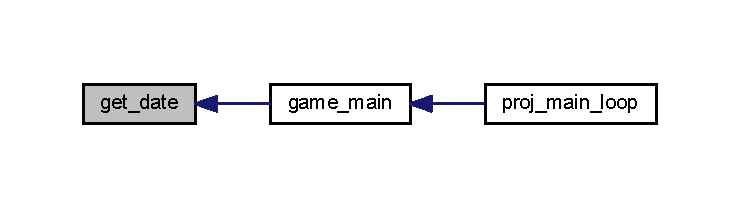
\includegraphics[width=350pt]{group__rtc_ga1f2c4f317d879fe00426ee4317bc625f_icgraph}
\end{center}
\end{figure}
\mbox{\Hypertarget{group__rtc_ga6222d2da81f961f574c428db117e610e}\label{group__rtc_ga6222d2da81f961f574c428db117e610e}} 
\index{rtc@{rtc}!rtc\+\_\+disable\+\_\+update\+\_\+ints@{rtc\+\_\+disable\+\_\+update\+\_\+ints}}
\index{rtc\+\_\+disable\+\_\+update\+\_\+ints@{rtc\+\_\+disable\+\_\+update\+\_\+ints}!rtc@{rtc}}
\subsubsection{\texorpdfstring{rtc\+\_\+disable\+\_\+update\+\_\+ints()}{rtc\_disable\_update\_ints()}}
{\footnotesize\ttfamily int rtc\+\_\+disable\+\_\+update\+\_\+ints (\begin{DoxyParamCaption}{ }\end{DoxyParamCaption})}



Disables update-\/ended interruptions. 

\begin{DoxyReturn}{Returns}
int -\/ Return 0 upon success and non-\/zero otherwise 
\end{DoxyReturn}
Here is the call graph for this function\+:
\nopagebreak
\begin{figure}[H]
\begin{center}
\leavevmode
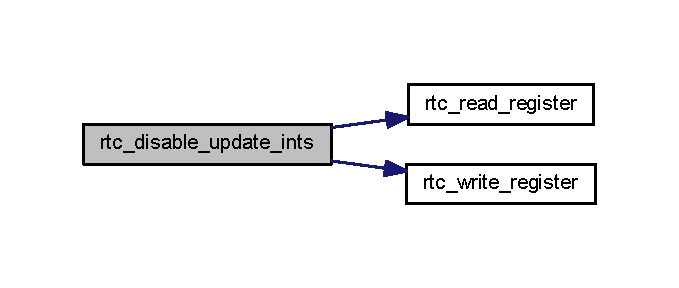
\includegraphics[width=326pt]{group__rtc_ga6222d2da81f961f574c428db117e610e_cgraph}
\end{center}
\end{figure}
Here is the caller graph for this function\+:
\nopagebreak
\begin{figure}[H]
\begin{center}
\leavevmode
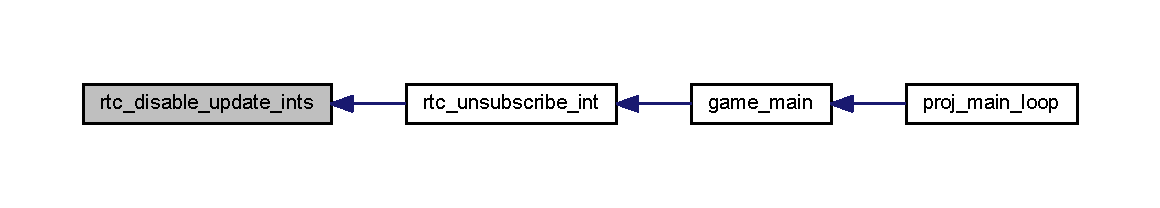
\includegraphics[width=350pt]{group__rtc_ga6222d2da81f961f574c428db117e610e_icgraph}
\end{center}
\end{figure}
\mbox{\Hypertarget{group__rtc_ga33036209deeaa3ca32027fdab0c8b2d7}\label{group__rtc_ga33036209deeaa3ca32027fdab0c8b2d7}} 
\index{rtc@{rtc}!rtc\+\_\+enable\+\_\+update\+\_\+ints@{rtc\+\_\+enable\+\_\+update\+\_\+ints}}
\index{rtc\+\_\+enable\+\_\+update\+\_\+ints@{rtc\+\_\+enable\+\_\+update\+\_\+ints}!rtc@{rtc}}
\subsubsection{\texorpdfstring{rtc\+\_\+enable\+\_\+update\+\_\+ints()}{rtc\_enable\_update\_ints()}}
{\footnotesize\ttfamily int rtc\+\_\+enable\+\_\+update\+\_\+ints (\begin{DoxyParamCaption}{ }\end{DoxyParamCaption})}



Enables update-\/ended interruptions. 

\begin{DoxyReturn}{Returns}
int -\/ Return 0 upon success and non-\/zero otherwise 
\end{DoxyReturn}
Here is the call graph for this function\+:
\nopagebreak
\begin{figure}[H]
\begin{center}
\leavevmode
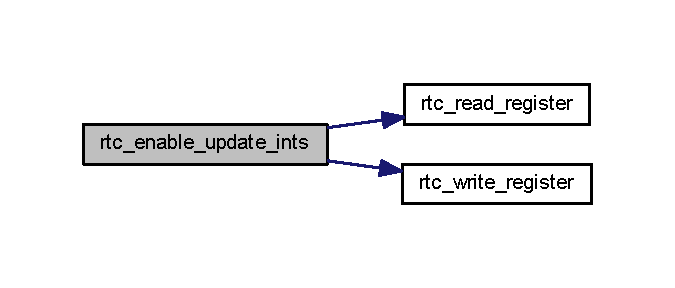
\includegraphics[width=324pt]{group__rtc_ga33036209deeaa3ca32027fdab0c8b2d7_cgraph}
\end{center}
\end{figure}
Here is the caller graph for this function\+:
\nopagebreak
\begin{figure}[H]
\begin{center}
\leavevmode
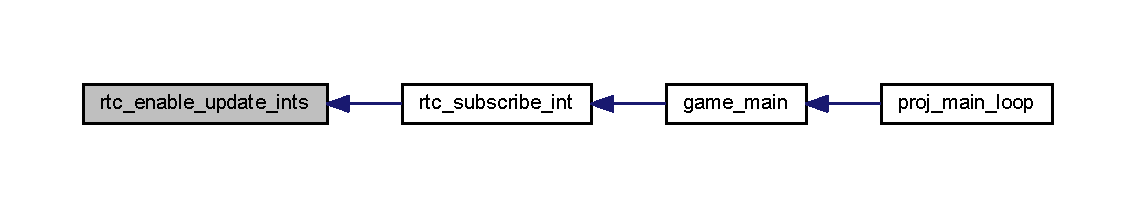
\includegraphics[width=350pt]{group__rtc_ga33036209deeaa3ca32027fdab0c8b2d7_icgraph}
\end{center}
\end{figure}
\mbox{\Hypertarget{group__rtc_ga75dad42881d64cf07cf1bdc2979a7056}\label{group__rtc_ga75dad42881d64cf07cf1bdc2979a7056}} 
\index{rtc@{rtc}!rtc\+\_\+ih@{rtc\+\_\+ih}}
\index{rtc\+\_\+ih@{rtc\+\_\+ih}!rtc@{rtc}}
\subsubsection{\texorpdfstring{rtc\+\_\+ih()}{rtc\_ih()}}
{\footnotesize\ttfamily void rtc\+\_\+ih (\begin{DoxyParamCaption}{ }\end{DoxyParamCaption})}



R\+TC interrupt handler, reads register C to verify what is the source of the interruptions and handles the information accordingly. 

Here is the call graph for this function\+:
\nopagebreak
\begin{figure}[H]
\begin{center}
\leavevmode
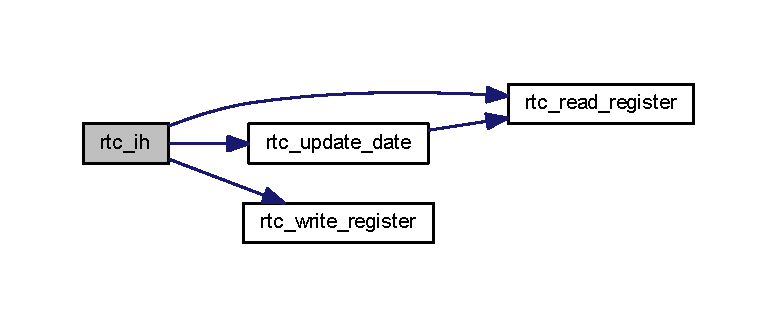
\includegraphics[width=350pt]{group__rtc_ga75dad42881d64cf07cf1bdc2979a7056_cgraph}
\end{center}
\end{figure}
Here is the caller graph for this function\+:
\nopagebreak
\begin{figure}[H]
\begin{center}
\leavevmode
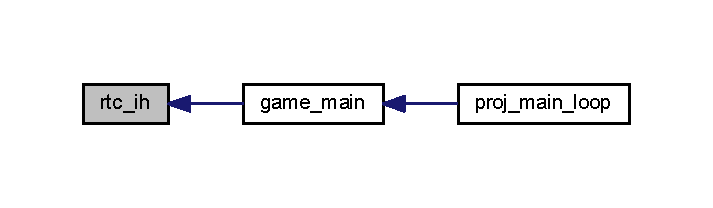
\includegraphics[width=342pt]{group__rtc_ga75dad42881d64cf07cf1bdc2979a7056_icgraph}
\end{center}
\end{figure}
\mbox{\Hypertarget{group__rtc_ga59359f9460af7b7dce7a2c8dc9d98211}\label{group__rtc_ga59359f9460af7b7dce7a2c8dc9d98211}} 
\index{rtc@{rtc}!rtc\+\_\+read\+\_\+day\+\_\+month@{rtc\+\_\+read\+\_\+day\+\_\+month}}
\index{rtc\+\_\+read\+\_\+day\+\_\+month@{rtc\+\_\+read\+\_\+day\+\_\+month}!rtc@{rtc}}
\subsubsection{\texorpdfstring{rtc\+\_\+read\+\_\+day\+\_\+month()}{rtc\_read\_day\_month()}}
{\footnotesize\ttfamily uint32\+\_\+t rtc\+\_\+read\+\_\+day\+\_\+month (\begin{DoxyParamCaption}{ }\end{DoxyParamCaption})}



Reads day of the month from the appropriate register. 

\begin{DoxyReturn}{Returns}
uint32\+\_\+t -\/ Returns the day of the month in the B\+CD format 
\end{DoxyReturn}
Here is the call graph for this function\+:
\nopagebreak
\begin{figure}[H]
\begin{center}
\leavevmode
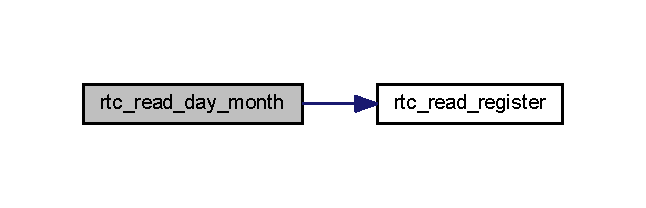
\includegraphics[width=310pt]{group__rtc_ga59359f9460af7b7dce7a2c8dc9d98211_cgraph}
\end{center}
\end{figure}
\mbox{\Hypertarget{group__rtc_ga2e585f34d69246a60a1db0e94ca09c05}\label{group__rtc_ga2e585f34d69246a60a1db0e94ca09c05}} 
\index{rtc@{rtc}!rtc\+\_\+read\+\_\+day\+\_\+week@{rtc\+\_\+read\+\_\+day\+\_\+week}}
\index{rtc\+\_\+read\+\_\+day\+\_\+week@{rtc\+\_\+read\+\_\+day\+\_\+week}!rtc@{rtc}}
\subsubsection{\texorpdfstring{rtc\+\_\+read\+\_\+day\+\_\+week()}{rtc\_read\_day\_week()}}
{\footnotesize\ttfamily uint32\+\_\+t rtc\+\_\+read\+\_\+day\+\_\+week (\begin{DoxyParamCaption}{ }\end{DoxyParamCaption})}



Reads day of the week from the appropriate register. 

\begin{DoxyReturn}{Returns}
uint32\+\_\+t -\/ Returns the day of the week in the B\+CD format 
\end{DoxyReturn}
Here is the call graph for this function\+:
\nopagebreak
\begin{figure}[H]
\begin{center}
\leavevmode
\includegraphics[width=306pt]{group__rtc_ga2e585f34d69246a60a1db0e94ca09c05_cgraph}
\end{center}
\end{figure}
\mbox{\Hypertarget{group__rtc_ga512adcbde067ca5bb83b1af0e0a7a444}\label{group__rtc_ga512adcbde067ca5bb83b1af0e0a7a444}} 
\index{rtc@{rtc}!rtc\+\_\+read\+\_\+hours@{rtc\+\_\+read\+\_\+hours}}
\index{rtc\+\_\+read\+\_\+hours@{rtc\+\_\+read\+\_\+hours}!rtc@{rtc}}
\subsubsection{\texorpdfstring{rtc\+\_\+read\+\_\+hours()}{rtc\_read\_hours()}}
{\footnotesize\ttfamily uint32\+\_\+t rtc\+\_\+read\+\_\+hours (\begin{DoxyParamCaption}{ }\end{DoxyParamCaption})}



Reads hour from the appropriate register. 

\begin{DoxyReturn}{Returns}
uint32\+\_\+t -\/ Returns the hour in the B\+CD format 
\end{DoxyReturn}
Here is the call graph for this function\+:
\nopagebreak
\begin{figure}[H]
\begin{center}
\leavevmode
\includegraphics[width=286pt]{group__rtc_ga512adcbde067ca5bb83b1af0e0a7a444_cgraph}
\end{center}
\end{figure}
\mbox{\Hypertarget{group__rtc_gaac43b2266aa06ad5a572d0fa3976ebb0}\label{group__rtc_gaac43b2266aa06ad5a572d0fa3976ebb0}} 
\index{rtc@{rtc}!rtc\+\_\+read\+\_\+minutes@{rtc\+\_\+read\+\_\+minutes}}
\index{rtc\+\_\+read\+\_\+minutes@{rtc\+\_\+read\+\_\+minutes}!rtc@{rtc}}
\subsubsection{\texorpdfstring{rtc\+\_\+read\+\_\+minutes()}{rtc\_read\_minutes()}}
{\footnotesize\ttfamily uint32\+\_\+t rtc\+\_\+read\+\_\+minutes (\begin{DoxyParamCaption}{ }\end{DoxyParamCaption})}



Reads minutes from the appropriate register. 

\begin{DoxyReturn}{Returns}
uint32\+\_\+t -\/ Returns the minutes in the B\+CD format 
\end{DoxyReturn}
Here is the call graph for this function\+:
\nopagebreak
\begin{figure}[H]
\begin{center}
\leavevmode
\includegraphics[width=297pt]{group__rtc_gaac43b2266aa06ad5a572d0fa3976ebb0_cgraph}
\end{center}
\end{figure}
\mbox{\Hypertarget{group__rtc_gabd90445bf474121fa89636a17f4c7369}\label{group__rtc_gabd90445bf474121fa89636a17f4c7369}} 
\index{rtc@{rtc}!rtc\+\_\+read\+\_\+month@{rtc\+\_\+read\+\_\+month}}
\index{rtc\+\_\+read\+\_\+month@{rtc\+\_\+read\+\_\+month}!rtc@{rtc}}
\subsubsection{\texorpdfstring{rtc\+\_\+read\+\_\+month()}{rtc\_read\_month()}}
{\footnotesize\ttfamily uint32\+\_\+t rtc\+\_\+read\+\_\+month (\begin{DoxyParamCaption}{ }\end{DoxyParamCaption})}



Reads month from the appropriate register. 

\begin{DoxyReturn}{Returns}
uint32\+\_\+t -\/ Returns the month in the B\+CD format 
\end{DoxyReturn}
Here is the call graph for this function\+:
\nopagebreak
\begin{figure}[H]
\begin{center}
\leavevmode
\includegraphics[width=289pt]{group__rtc_gabd90445bf474121fa89636a17f4c7369_cgraph}
\end{center}
\end{figure}
\mbox{\Hypertarget{group__rtc_gaf6f18245f611a9c8f64055feae5ec73d}\label{group__rtc_gaf6f18245f611a9c8f64055feae5ec73d}} 
\index{rtc@{rtc}!rtc\+\_\+read\+\_\+register@{rtc\+\_\+read\+\_\+register}}
\index{rtc\+\_\+read\+\_\+register@{rtc\+\_\+read\+\_\+register}!rtc@{rtc}}
\subsubsection{\texorpdfstring{rtc\+\_\+read\+\_\+register()}{rtc\_read\_register()}}
{\footnotesize\ttfamily int rtc\+\_\+read\+\_\+register (\begin{DoxyParamCaption}\item[{uint32\+\_\+t}]{addr,  }\item[{uint32\+\_\+t $\ast$}]{data }\end{DoxyParamCaption})}



Reads R\+TC address passed in the arguments and stores it. 


\begin{DoxyParams}{Parameters}
{\em addr} & -\/ R\+TC address to be accessed and read \\
\hline
{\em data} & -\/ pointer to the location where data will be stored \\
\hline
\end{DoxyParams}
\begin{DoxyReturn}{Returns}
int -\/ Return 0 upon success and non-\/zero otherwise 
\end{DoxyReturn}
Here is the caller graph for this function\+:
\nopagebreak
\begin{figure}[H]
\begin{center}
\leavevmode
\includegraphics[width=350pt]{group__rtc_gaf6f18245f611a9c8f64055feae5ec73d_icgraph}
\end{center}
\end{figure}
\mbox{\Hypertarget{group__rtc_ga3d9330b99a772073f924e69bc1b2df05}\label{group__rtc_ga3d9330b99a772073f924e69bc1b2df05}} 
\index{rtc@{rtc}!rtc\+\_\+read\+\_\+seconds@{rtc\+\_\+read\+\_\+seconds}}
\index{rtc\+\_\+read\+\_\+seconds@{rtc\+\_\+read\+\_\+seconds}!rtc@{rtc}}
\subsubsection{\texorpdfstring{rtc\+\_\+read\+\_\+seconds()}{rtc\_read\_seconds()}}
{\footnotesize\ttfamily uint32\+\_\+t rtc\+\_\+read\+\_\+seconds (\begin{DoxyParamCaption}{ }\end{DoxyParamCaption})}



Reads seconds from the appropriate register. 

\begin{DoxyReturn}{Returns}
uint32\+\_\+t -\/ Returns the seconds in the B\+CD format 
\end{DoxyReturn}
Here is the call graph for this function\+:
\nopagebreak
\begin{figure}[H]
\begin{center}
\leavevmode
\includegraphics[width=299pt]{group__rtc_ga3d9330b99a772073f924e69bc1b2df05_cgraph}
\end{center}
\end{figure}
\mbox{\Hypertarget{group__rtc_ga4ddd82a19df760d95b2dd0c92ec6c63b}\label{group__rtc_ga4ddd82a19df760d95b2dd0c92ec6c63b}} 
\index{rtc@{rtc}!rtc\+\_\+read\+\_\+year@{rtc\+\_\+read\+\_\+year}}
\index{rtc\+\_\+read\+\_\+year@{rtc\+\_\+read\+\_\+year}!rtc@{rtc}}
\subsubsection{\texorpdfstring{rtc\+\_\+read\+\_\+year()}{rtc\_read\_year()}}
{\footnotesize\ttfamily uint32\+\_\+t rtc\+\_\+read\+\_\+year (\begin{DoxyParamCaption}{ }\end{DoxyParamCaption})}



Reads year from the appropriate register. 

\begin{DoxyReturn}{Returns}
uint32\+\_\+t -\/ Returns the year in the B\+CD format 
\end{DoxyReturn}
Here is the call graph for this function\+:
\nopagebreak
\begin{figure}[H]
\begin{center}
\leavevmode
\includegraphics[width=281pt]{group__rtc_ga4ddd82a19df760d95b2dd0c92ec6c63b_cgraph}
\end{center}
\end{figure}
\mbox{\Hypertarget{group__rtc_ga7c28e3528db0f743706f9c01608331a7}\label{group__rtc_ga7c28e3528db0f743706f9c01608331a7}} 
\index{rtc@{rtc}!rtc\+\_\+subscribe\+\_\+int@{rtc\+\_\+subscribe\+\_\+int}}
\index{rtc\+\_\+subscribe\+\_\+int@{rtc\+\_\+subscribe\+\_\+int}!rtc@{rtc}}
\subsubsection{\texorpdfstring{rtc\+\_\+subscribe\+\_\+int()}{rtc\_subscribe\_int()}}
{\footnotesize\ttfamily int rtc\+\_\+subscribe\+\_\+int (\begin{DoxyParamCaption}\item[{uint8\+\_\+t $\ast$}]{bitno }\end{DoxyParamCaption})}



Subscribes R\+TC interruptions. 


\begin{DoxyParams}{Parameters}
{\em bitno} & -\/ address of memory to be initialized with the bit number to be set in the mask returned upon an interrupt \\
\hline
\end{DoxyParams}
\begin{DoxyReturn}{Returns}
int -\/ Return 0 upon success and non-\/zero otherwise 
\end{DoxyReturn}
Here is the call graph for this function\+:
\nopagebreak
\begin{figure}[H]
\begin{center}
\leavevmode
\includegraphics[width=350pt]{group__rtc_ga7c28e3528db0f743706f9c01608331a7_cgraph}
\end{center}
\end{figure}
Here is the caller graph for this function\+:
\nopagebreak
\begin{figure}[H]
\begin{center}
\leavevmode
\includegraphics[width=350pt]{group__rtc_ga7c28e3528db0f743706f9c01608331a7_icgraph}
\end{center}
\end{figure}
\mbox{\Hypertarget{group__rtc_gab8f17bf5280c908c8b199a90fefcc758}\label{group__rtc_gab8f17bf5280c908c8b199a90fefcc758}} 
\index{rtc@{rtc}!rtc\+\_\+unsubscribe\+\_\+int@{rtc\+\_\+unsubscribe\+\_\+int}}
\index{rtc\+\_\+unsubscribe\+\_\+int@{rtc\+\_\+unsubscribe\+\_\+int}!rtc@{rtc}}
\subsubsection{\texorpdfstring{rtc\+\_\+unsubscribe\+\_\+int()}{rtc\_unsubscribe\_int()}}
{\footnotesize\ttfamily int rtc\+\_\+unsubscribe\+\_\+int (\begin{DoxyParamCaption}{ }\end{DoxyParamCaption})}



Unsubscribes R\+TC interruptions. 

\begin{DoxyReturn}{Returns}
int -\/ Return 0 upon success and non-\/zero otherwise 
\end{DoxyReturn}
Here is the call graph for this function\+:
\nopagebreak
\begin{figure}[H]
\begin{center}
\leavevmode
\includegraphics[width=350pt]{group__rtc_gab8f17bf5280c908c8b199a90fefcc758_cgraph}
\end{center}
\end{figure}
Here is the caller graph for this function\+:
\nopagebreak
\begin{figure}[H]
\begin{center}
\leavevmode
\includegraphics[width=350pt]{group__rtc_gab8f17bf5280c908c8b199a90fefcc758_icgraph}
\end{center}
\end{figure}
\mbox{\Hypertarget{group__rtc_ga1c7900b102529826ac1662355e6cf058}\label{group__rtc_ga1c7900b102529826ac1662355e6cf058}} 
\index{rtc@{rtc}!rtc\+\_\+update\+\_\+date@{rtc\+\_\+update\+\_\+date}}
\index{rtc\+\_\+update\+\_\+date@{rtc\+\_\+update\+\_\+date}!rtc@{rtc}}
\subsubsection{\texorpdfstring{rtc\+\_\+update\+\_\+date()}{rtc\_update\_date()}}
{\footnotesize\ttfamily int rtc\+\_\+update\+\_\+date (\begin{DoxyParamCaption}{ }\end{DoxyParamCaption})}



Update the \mbox{\hyperlink{struct_date}{Date}} object with new information. 

\begin{DoxyReturn}{Returns}
int -\/ Return 0 upon success and non-\/zero otherwise 
\end{DoxyReturn}
Here is the call graph for this function\+:
\nopagebreak
\begin{figure}[H]
\begin{center}
\leavevmode
\includegraphics[width=291pt]{group__rtc_ga1c7900b102529826ac1662355e6cf058_cgraph}
\end{center}
\end{figure}
Here is the caller graph for this function\+:
\nopagebreak
\begin{figure}[H]
\begin{center}
\leavevmode
\includegraphics[width=350pt]{group__rtc_ga1c7900b102529826ac1662355e6cf058_icgraph}
\end{center}
\end{figure}
\mbox{\Hypertarget{group__rtc_ga9b5d85527d676067a8c05780ec46d4f1}\label{group__rtc_ga9b5d85527d676067a8c05780ec46d4f1}} 
\index{rtc@{rtc}!rtc\+\_\+write\+\_\+register@{rtc\+\_\+write\+\_\+register}}
\index{rtc\+\_\+write\+\_\+register@{rtc\+\_\+write\+\_\+register}!rtc@{rtc}}
\subsubsection{\texorpdfstring{rtc\+\_\+write\+\_\+register()}{rtc\_write\_register()}}
{\footnotesize\ttfamily int rtc\+\_\+write\+\_\+register (\begin{DoxyParamCaption}\item[{uint32\+\_\+t}]{addr,  }\item[{uint32\+\_\+t}]{data }\end{DoxyParamCaption})}



Writes to the R\+TC address passed in the arguments. 


\begin{DoxyParams}{Parameters}
{\em addr} & -\/ R\+TC address to be accesed and altered \\
\hline
{\em data} & -\/ Data to be written to the register \\
\hline
\end{DoxyParams}
\begin{DoxyReturn}{Returns}
int -\/ Return 0 upon success and non-\/zero otherwise 
\end{DoxyReturn}
Here is the caller graph for this function\+:
\nopagebreak
\begin{figure}[H]
\begin{center}
\leavevmode
\includegraphics[width=350pt]{group__rtc_ga9b5d85527d676067a8c05780ec46d4f1_icgraph}
\end{center}
\end{figure}


\subsection{Variable Documentation}
\mbox{\Hypertarget{group__rtc_ga897ed87b95b7a37afeeb935ca0b2366b}\label{group__rtc_ga897ed87b95b7a37afeeb935ca0b2366b}} 
\index{rtc@{rtc}!day@{day}}
\index{day@{day}!rtc@{rtc}}
\subsubsection{\texorpdfstring{day}{day}}
{\footnotesize\ttfamily uint32\+\_\+t day}

\mbox{\Hypertarget{group__rtc_gaa24f12f79f7553236083be08521c546e}\label{group__rtc_gaa24f12f79f7553236083be08521c546e}} 
\index{rtc@{rtc}!dayW@{dayW}}
\index{dayW@{dayW}!rtc@{rtc}}
\subsubsection{\texorpdfstring{dayW}{dayW}}
{\footnotesize\ttfamily uint32\+\_\+t dayW}

\mbox{\Hypertarget{group__rtc_ga26d5bae76d83086900174b266fd2cd82}\label{group__rtc_ga26d5bae76d83086900174b266fd2cd82}} 
\index{rtc@{rtc}!hour@{hour}}
\index{hour@{hour}!rtc@{rtc}}
\subsubsection{\texorpdfstring{hour}{hour}}
{\footnotesize\ttfamily uint32\+\_\+t hour}

\mbox{\Hypertarget{group__rtc_ga2dcb690348d97b756f4d165c80c9af7d}\label{group__rtc_ga2dcb690348d97b756f4d165c80c9af7d}} 
\index{rtc@{rtc}!minutes@{minutes}}
\index{minutes@{minutes}!rtc@{rtc}}
\subsubsection{\texorpdfstring{minutes}{minutes}}
{\footnotesize\ttfamily uint32\+\_\+t minutes}

\mbox{\Hypertarget{group__rtc_ga55a5fa57878363d803833666ddf3c16f}\label{group__rtc_ga55a5fa57878363d803833666ddf3c16f}} 
\index{rtc@{rtc}!month@{month}}
\index{month@{month}!rtc@{rtc}}
\subsubsection{\texorpdfstring{month}{month}}
{\footnotesize\ttfamily uint32\+\_\+t month}

\mbox{\Hypertarget{group__rtc_ga6d5694839ec935781627e5c52de21fda}\label{group__rtc_ga6d5694839ec935781627e5c52de21fda}} 
\index{rtc@{rtc}!seconds@{seconds}}
\index{seconds@{seconds}!rtc@{rtc}}
\subsubsection{\texorpdfstring{seconds}{seconds}}
{\footnotesize\ttfamily uint32\+\_\+t seconds}

\mbox{\Hypertarget{group__rtc_gaac3a162d2f192fe2360aba534eac7198}\label{group__rtc_gaac3a162d2f192fe2360aba534eac7198}} 
\index{rtc@{rtc}!year@{year}}
\index{year@{year}!rtc@{rtc}}
\subsubsection{\texorpdfstring{year}{year}}
{\footnotesize\ttfamily uint32\+\_\+t year}


\hypertarget{group__tetramino}{}\section{tetramino}
\label{group__tetramino}\index{tetramino@{tetramino}}
\subsection*{Data Structures}
\begin{DoxyCompactItemize}
\item 
struct \mbox{\hyperlink{struct_square}{Square}}
\item 
struct \mbox{\hyperlink{struct_board}{Board}}
\item 
struct \mbox{\hyperlink{struct_tetramino}{Tetramino}}
\end{DoxyCompactItemize}
\subsection*{Macros}
\begin{DoxyCompactItemize}
\item 
\#define \mbox{\hyperlink{group__tetramino_ga70ed59adcb4159ac551058053e649640}{S\+I\+ZE}}~20
\item 
\#define \mbox{\hyperlink{group__tetramino_gaf53d889f840b107b1a7ffd5534d8a484}{S\+O\+U\+T\+H\+\_\+\+B\+O\+R\+D\+ER}}~580
\item 
\#define \mbox{\hyperlink{group__tetramino_ga3aca436a21c820e0632d5d815a520189}{N\+O\+R\+T\+H\+\_\+\+B\+O\+R\+D\+ER}}~160
\item 
\#define \mbox{\hyperlink{group__tetramino_gaec71d31827b6eb16515454097e75cf12}{E\+A\+S\+T\+\_\+\+B\+O\+R\+D\+ER}}~550
\item 
\#define \mbox{\hyperlink{group__tetramino_gae6a8f15a920bce5c0cbcf2577915268e}{W\+E\+S\+T\+\_\+\+B\+O\+R\+D\+ER}}~230
\item 
\#define \mbox{\hyperlink{group__tetramino_gab6ccafbecf8edd9189e074574b652c91}{M\+O\+V\+E\+\_\+\+D\+O\+WN}}~true
\item 
\#define \mbox{\hyperlink{group__tetramino_gac6d51f1ce7e6114465d635e6b8411d2c}{M\+A\+X\+\_\+\+B\+O\+A\+RD}}~299
\end{DoxyCompactItemize}
\subsection*{Functions}
\begin{DoxyCompactItemize}
\item 
uint16\+\_\+t \mbox{\hyperlink{group__tetramino_gaec1f53f8b300eba51c8863f3fcb5478b}{choose\+\_\+color}} (int shape\+\_\+n)
\begin{DoxyCompactList}\small\item\em Chooses the color of the piece according to its shape. \end{DoxyCompactList}\item 
bool \mbox{\hyperlink{group__tetramino_gaed055860f4584eb217234f06c29d3ab4}{check\+\_\+for\+\_\+gameover}} (\mbox{\hyperlink{struct_board}{Board}} $\ast$board)
\begin{DoxyCompactList}\small\item\em Checks the board current status and if the player has reached to gameover state. \end{DoxyCompactList}\item 
void \mbox{\hyperlink{group__tetramino_gaab50f02f99355b3ceb43290e186fe609}{check\+\_\+eliminate\+\_\+line}} (\mbox{\hyperlink{struct_tetramino}{Tetramino}} $\ast$t, int $\ast$pos)
\begin{DoxyCompactList}\small\item\em Check the lines where a \mbox{\hyperlink{struct_tetramino}{Tetramino}} lands to see if a line has been completed. \end{DoxyCompactList}\item 
void \mbox{\hyperlink{group__tetramino_ga2f2a68722efc3ecbd82eea0a337f6b7f}{update\+\_\+board\+\_\+after\+\_\+line}} (\mbox{\hyperlink{struct_board}{Board}} $\ast$bd, int position)
\begin{DoxyCompactList}\small\item\em Updates the board after a line has been removed. \end{DoxyCompactList}\item 
void \mbox{\hyperlink{group__tetramino_ga64e78e0b93dcd6d9b3092b4b8d1fd339}{draw\+\_\+squares}} (\mbox{\hyperlink{struct_board}{Board}} $\ast$bd)
\begin{DoxyCompactList}\small\item\em Draws all squares of the board, painting it black the empty positions and non-\/black those who belong to tetraminos. \end{DoxyCompactList}\item 
\mbox{\hyperlink{struct_tetramino}{Tetramino}} $\ast$ \mbox{\hyperlink{group__tetramino_ga9a2309ca24e8dec1a1bf31a995db2de1}{new\+\_\+tetramino}} (\mbox{\hyperlink{struct_board}{Board}} $\ast$board)
\begin{DoxyCompactList}\small\item\em Creates a new tetramino and loads initial information of the piece. \end{DoxyCompactList}\item 
\mbox{\hyperlink{struct_board}{Board}} $\ast$ \mbox{\hyperlink{group__tetramino_ga3d4977293a2989f9483b897b1a5bd073}{new\+\_\+board}} ()
\begin{DoxyCompactList}\small\item\em Creates a new board and loads initial information. \end{DoxyCompactList}\item 
void \mbox{\hyperlink{group__tetramino_ga5ab138241d19c1826240ea803c970d9d}{delete\+\_\+board}} (\mbox{\hyperlink{struct_board}{Board}} $\ast$board)
\begin{DoxyCompactList}\small\item\em Deletes a board and frees the memory allocated to the struct. \end{DoxyCompactList}\item 
void \mbox{\hyperlink{group__tetramino_ga562ee8dcd3b145bafdf0311f1a3b7296}{delete\+\_\+tetramino}} (\mbox{\hyperlink{struct_tetramino}{Tetramino}} $\ast$t)
\begin{DoxyCompactList}\small\item\em Deletes a tetramino and frees the memory alloacted to the struct. \end{DoxyCompactList}\end{DoxyCompactItemize}
\subsection*{Variables}
\begin{DoxyCompactItemize}
\item 
uint16\+\_\+t \mbox{\hyperlink{group__tetramino_ga4dde988b1b2adba65ae3efa69f65d960}{x}}
\item 
uint16\+\_\+t \mbox{\hyperlink{group__tetramino_gab0580f504a7428539be299fa71565f30}{y}}
\item 
uint16\+\_\+t \mbox{\hyperlink{group__tetramino_ga0b10c5b0fa8e65e009263b93ba2671ae}{color}}
\item 
\mbox{\hyperlink{struct_square}{Square}} \mbox{\hyperlink{group__tetramino_ga4eedd16e00191125d9b7c28eed681ef4}{positions}} \mbox{[}300\mbox{]}
\item 
uint16\+\_\+t \mbox{\hyperlink{group__tetramino_gad0eab1042455a2067c812ab8071d5376}{width}}
\item 
uint16\+\_\+t \mbox{\hyperlink{group__tetramino_ga81c9f8d0b8c3b49d770be14dbe9f0d37}{height}}
\item 
uint16\+\_\+t \mbox{\hyperlink{group__tetramino_ga92d26140c764e05f62f37639fb87fc88}{x\+\_\+gini}}
\item 
uint16\+\_\+t \mbox{\hyperlink{group__tetramino_gafccac8a8a85671bdaf9a927aaefb0b05}{y\+\_\+gini}}
\item 
uint16\+\_\+t \mbox{\hyperlink{group__tetramino_ga9d0491d7027bf54689b51ff9e57b3703}{sqidx}} \mbox{[}4\mbox{]}
\item 
uint16\+\_\+t \mbox{\hyperlink{group__tetramino_ga0b10c5b0fa8e65e009263b93ba2671ae}{color}}
\item 
int \mbox{\hyperlink{group__tetramino_gae4edf8f6630ef7f8b4c587348a3001a7}{rot}}
\item 
\mbox{\hyperlink{struct_board}{Board}} $\ast$ \mbox{\hyperlink{group__tetramino_ga30c121d94ba906148e5a4b0546e723a3}{bd}}
\item 
int \mbox{\hyperlink{group__tetramino_ga7aa41fc2efed4bde82530b155c4000f1}{shape\+\_\+n}}
\end{DoxyCompactItemize}


\subsection{Detailed Description}
Functions for manipulating tetraminos and board 

\subsection{Macro Definition Documentation}
\mbox{\Hypertarget{group__tetramino_gaec71d31827b6eb16515454097e75cf12}\label{group__tetramino_gaec71d31827b6eb16515454097e75cf12}} 
\index{tetramino@{tetramino}!E\+A\+S\+T\+\_\+\+B\+O\+R\+D\+ER@{E\+A\+S\+T\+\_\+\+B\+O\+R\+D\+ER}}
\index{E\+A\+S\+T\+\_\+\+B\+O\+R\+D\+ER@{E\+A\+S\+T\+\_\+\+B\+O\+R\+D\+ER}!tetramino@{tetramino}}
\subsubsection{\texorpdfstring{E\+A\+S\+T\+\_\+\+B\+O\+R\+D\+ER}{EAST\_BORDER}}
{\footnotesize\ttfamily \#define E\+A\+S\+T\+\_\+\+B\+O\+R\+D\+ER~550}

\mbox{\Hypertarget{group__tetramino_gac6d51f1ce7e6114465d635e6b8411d2c}\label{group__tetramino_gac6d51f1ce7e6114465d635e6b8411d2c}} 
\index{tetramino@{tetramino}!M\+A\+X\+\_\+\+B\+O\+A\+RD@{M\+A\+X\+\_\+\+B\+O\+A\+RD}}
\index{M\+A\+X\+\_\+\+B\+O\+A\+RD@{M\+A\+X\+\_\+\+B\+O\+A\+RD}!tetramino@{tetramino}}
\subsubsection{\texorpdfstring{M\+A\+X\+\_\+\+B\+O\+A\+RD}{MAX\_BOARD}}
{\footnotesize\ttfamily \#define M\+A\+X\+\_\+\+B\+O\+A\+RD~299}

\mbox{\Hypertarget{group__tetramino_gab6ccafbecf8edd9189e074574b652c91}\label{group__tetramino_gab6ccafbecf8edd9189e074574b652c91}} 
\index{tetramino@{tetramino}!M\+O\+V\+E\+\_\+\+D\+O\+WN@{M\+O\+V\+E\+\_\+\+D\+O\+WN}}
\index{M\+O\+V\+E\+\_\+\+D\+O\+WN@{M\+O\+V\+E\+\_\+\+D\+O\+WN}!tetramino@{tetramino}}
\subsubsection{\texorpdfstring{M\+O\+V\+E\+\_\+\+D\+O\+WN}{MOVE\_DOWN}}
{\footnotesize\ttfamily \#define M\+O\+V\+E\+\_\+\+D\+O\+WN~true}

\mbox{\Hypertarget{group__tetramino_ga3aca436a21c820e0632d5d815a520189}\label{group__tetramino_ga3aca436a21c820e0632d5d815a520189}} 
\index{tetramino@{tetramino}!N\+O\+R\+T\+H\+\_\+\+B\+O\+R\+D\+ER@{N\+O\+R\+T\+H\+\_\+\+B\+O\+R\+D\+ER}}
\index{N\+O\+R\+T\+H\+\_\+\+B\+O\+R\+D\+ER@{N\+O\+R\+T\+H\+\_\+\+B\+O\+R\+D\+ER}!tetramino@{tetramino}}
\subsubsection{\texorpdfstring{N\+O\+R\+T\+H\+\_\+\+B\+O\+R\+D\+ER}{NORTH\_BORDER}}
{\footnotesize\ttfamily \#define N\+O\+R\+T\+H\+\_\+\+B\+O\+R\+D\+ER~160}

\mbox{\Hypertarget{group__tetramino_ga70ed59adcb4159ac551058053e649640}\label{group__tetramino_ga70ed59adcb4159ac551058053e649640}} 
\index{tetramino@{tetramino}!S\+I\+ZE@{S\+I\+ZE}}
\index{S\+I\+ZE@{S\+I\+ZE}!tetramino@{tetramino}}
\subsubsection{\texorpdfstring{S\+I\+ZE}{SIZE}}
{\footnotesize\ttfamily \#define S\+I\+ZE~20}

\mbox{\Hypertarget{group__tetramino_gaf53d889f840b107b1a7ffd5534d8a484}\label{group__tetramino_gaf53d889f840b107b1a7ffd5534d8a484}} 
\index{tetramino@{tetramino}!S\+O\+U\+T\+H\+\_\+\+B\+O\+R\+D\+ER@{S\+O\+U\+T\+H\+\_\+\+B\+O\+R\+D\+ER}}
\index{S\+O\+U\+T\+H\+\_\+\+B\+O\+R\+D\+ER@{S\+O\+U\+T\+H\+\_\+\+B\+O\+R\+D\+ER}!tetramino@{tetramino}}
\subsubsection{\texorpdfstring{S\+O\+U\+T\+H\+\_\+\+B\+O\+R\+D\+ER}{SOUTH\_BORDER}}
{\footnotesize\ttfamily \#define S\+O\+U\+T\+H\+\_\+\+B\+O\+R\+D\+ER~580}

\mbox{\Hypertarget{group__tetramino_gae6a8f15a920bce5c0cbcf2577915268e}\label{group__tetramino_gae6a8f15a920bce5c0cbcf2577915268e}} 
\index{tetramino@{tetramino}!W\+E\+S\+T\+\_\+\+B\+O\+R\+D\+ER@{W\+E\+S\+T\+\_\+\+B\+O\+R\+D\+ER}}
\index{W\+E\+S\+T\+\_\+\+B\+O\+R\+D\+ER@{W\+E\+S\+T\+\_\+\+B\+O\+R\+D\+ER}!tetramino@{tetramino}}
\subsubsection{\texorpdfstring{W\+E\+S\+T\+\_\+\+B\+O\+R\+D\+ER}{WEST\_BORDER}}
{\footnotesize\ttfamily \#define W\+E\+S\+T\+\_\+\+B\+O\+R\+D\+ER~230}



\subsection{Function Documentation}
\mbox{\Hypertarget{group__tetramino_gaab50f02f99355b3ceb43290e186fe609}\label{group__tetramino_gaab50f02f99355b3ceb43290e186fe609}} 
\index{tetramino@{tetramino}!check\+\_\+eliminate\+\_\+line@{check\+\_\+eliminate\+\_\+line}}
\index{check\+\_\+eliminate\+\_\+line@{check\+\_\+eliminate\+\_\+line}!tetramino@{tetramino}}
\subsubsection{\texorpdfstring{check\+\_\+eliminate\+\_\+line()}{check\_eliminate\_line()}}
{\footnotesize\ttfamily void check\+\_\+eliminate\+\_\+line (\begin{DoxyParamCaption}\item[{\mbox{\hyperlink{struct_tetramino}{Tetramino}} $\ast$}]{t,  }\item[{int $\ast$}]{pos }\end{DoxyParamCaption})}



Check the lines where a \mbox{\hyperlink{struct_tetramino}{Tetramino}} lands to see if a line has been completed. 


\begin{DoxyParams}{Parameters}
{\em t} & -\/ Pointer to the tetramino struct \\
\hline
{\em pos} & -\/ Pointer to the array of positions \\
\hline
\end{DoxyParams}
Here is the caller graph for this function\+:
\nopagebreak
\begin{figure}[H]
\begin{center}
\leavevmode
\includegraphics[width=350pt]{group__tetramino_gaab50f02f99355b3ceb43290e186fe609_icgraph}
\end{center}
\end{figure}
\mbox{\Hypertarget{group__tetramino_gaed055860f4584eb217234f06c29d3ab4}\label{group__tetramino_gaed055860f4584eb217234f06c29d3ab4}} 
\index{tetramino@{tetramino}!check\+\_\+for\+\_\+gameover@{check\+\_\+for\+\_\+gameover}}
\index{check\+\_\+for\+\_\+gameover@{check\+\_\+for\+\_\+gameover}!tetramino@{tetramino}}
\subsubsection{\texorpdfstring{check\+\_\+for\+\_\+gameover()}{check\_for\_gameover()}}
{\footnotesize\ttfamily bool check\+\_\+for\+\_\+gameover (\begin{DoxyParamCaption}\item[{\mbox{\hyperlink{struct_board}{Board}} $\ast$}]{board }\end{DoxyParamCaption})}



Checks the board current status and if the player has reached to gameover state. 


\begin{DoxyParams}{Parameters}
{\em board} & -\/ Pointer to the board struct \\
\hline
\end{DoxyParams}
\begin{DoxyReturn}{Returns}
true -\/ If the player reached game over 

false -\/ If the player hasn\textquotesingle{}t reached the end game 
\end{DoxyReturn}
Here is the caller graph for this function\+:
\nopagebreak
\begin{figure}[H]
\begin{center}
\leavevmode
\includegraphics[width=350pt]{group__tetramino_gaed055860f4584eb217234f06c29d3ab4_icgraph}
\end{center}
\end{figure}
\mbox{\Hypertarget{group__tetramino_gaec1f53f8b300eba51c8863f3fcb5478b}\label{group__tetramino_gaec1f53f8b300eba51c8863f3fcb5478b}} 
\index{tetramino@{tetramino}!choose\+\_\+color@{choose\+\_\+color}}
\index{choose\+\_\+color@{choose\+\_\+color}!tetramino@{tetramino}}
\subsubsection{\texorpdfstring{choose\+\_\+color()}{choose\_color()}}
{\footnotesize\ttfamily uint16\+\_\+t choose\+\_\+color (\begin{DoxyParamCaption}\item[{int}]{shape\+\_\+n }\end{DoxyParamCaption})}



Chooses the color of the piece according to its shape. 


\begin{DoxyParams}{Parameters}
{\em shape\+\_\+n} & -\/ Identifies the piece shape \\
\hline
\end{DoxyParams}
\begin{DoxyReturn}{Returns}
uint16\+\_\+t -\/ Return the color in 16-\/bit mode 
\end{DoxyReturn}
Here is the caller graph for this function\+:
\nopagebreak
\begin{figure}[H]
\begin{center}
\leavevmode
\includegraphics[width=350pt]{group__tetramino_gaec1f53f8b300eba51c8863f3fcb5478b_icgraph}
\end{center}
\end{figure}
\mbox{\Hypertarget{group__tetramino_ga5ab138241d19c1826240ea803c970d9d}\label{group__tetramino_ga5ab138241d19c1826240ea803c970d9d}} 
\index{tetramino@{tetramino}!delete\+\_\+board@{delete\+\_\+board}}
\index{delete\+\_\+board@{delete\+\_\+board}!tetramino@{tetramino}}
\subsubsection{\texorpdfstring{delete\+\_\+board()}{delete\_board()}}
{\footnotesize\ttfamily void delete\+\_\+board (\begin{DoxyParamCaption}\item[{\mbox{\hyperlink{struct_board}{Board}} $\ast$}]{board }\end{DoxyParamCaption})}



Deletes a board and frees the memory allocated to the struct. 


\begin{DoxyParams}{Parameters}
{\em board} & -\/ Pointer to the board to be deleted \\
\hline
\end{DoxyParams}
Here is the caller graph for this function\+:
\nopagebreak
\begin{figure}[H]
\begin{center}
\leavevmode
\includegraphics[width=350pt]{group__tetramino_ga5ab138241d19c1826240ea803c970d9d_icgraph}
\end{center}
\end{figure}
\mbox{\Hypertarget{group__tetramino_ga562ee8dcd3b145bafdf0311f1a3b7296}\label{group__tetramino_ga562ee8dcd3b145bafdf0311f1a3b7296}} 
\index{tetramino@{tetramino}!delete\+\_\+tetramino@{delete\+\_\+tetramino}}
\index{delete\+\_\+tetramino@{delete\+\_\+tetramino}!tetramino@{tetramino}}
\subsubsection{\texorpdfstring{delete\+\_\+tetramino()}{delete\_tetramino()}}
{\footnotesize\ttfamily void delete\+\_\+tetramino (\begin{DoxyParamCaption}\item[{\mbox{\hyperlink{struct_tetramino}{Tetramino}} $\ast$}]{t }\end{DoxyParamCaption})}



Deletes a tetramino and frees the memory alloacted to the struct. 


\begin{DoxyParams}{Parameters}
{\em t} & -\/ Pointer to the tetramino to be deleted \\
\hline
\end{DoxyParams}
Here is the caller graph for this function\+:
\nopagebreak
\begin{figure}[H]
\begin{center}
\leavevmode
\includegraphics[width=350pt]{group__tetramino_ga562ee8dcd3b145bafdf0311f1a3b7296_icgraph}
\end{center}
\end{figure}
\mbox{\Hypertarget{group__tetramino_ga64e78e0b93dcd6d9b3092b4b8d1fd339}\label{group__tetramino_ga64e78e0b93dcd6d9b3092b4b8d1fd339}} 
\index{tetramino@{tetramino}!draw\+\_\+squares@{draw\+\_\+squares}}
\index{draw\+\_\+squares@{draw\+\_\+squares}!tetramino@{tetramino}}
\subsubsection{\texorpdfstring{draw\+\_\+squares()}{draw\_squares()}}
{\footnotesize\ttfamily void draw\+\_\+squares (\begin{DoxyParamCaption}\item[{\mbox{\hyperlink{struct_board}{Board}} $\ast$}]{bd }\end{DoxyParamCaption})}



Draws all squares of the board, painting it black the empty positions and non-\/black those who belong to tetraminos. 


\begin{DoxyParams}{Parameters}
{\em bd} & -\/ Pointer to the board \\
\hline
\end{DoxyParams}
Here is the call graph for this function\+:
\nopagebreak
\begin{figure}[H]
\begin{center}
\leavevmode
\includegraphics[width=350pt]{group__tetramino_ga64e78e0b93dcd6d9b3092b4b8d1fd339_cgraph}
\end{center}
\end{figure}
Here is the caller graph for this function\+:
\nopagebreak
\begin{figure}[H]
\begin{center}
\leavevmode
\includegraphics[width=350pt]{group__tetramino_ga64e78e0b93dcd6d9b3092b4b8d1fd339_icgraph}
\end{center}
\end{figure}
\mbox{\Hypertarget{group__tetramino_ga3d4977293a2989f9483b897b1a5bd073}\label{group__tetramino_ga3d4977293a2989f9483b897b1a5bd073}} 
\index{tetramino@{tetramino}!new\+\_\+board@{new\+\_\+board}}
\index{new\+\_\+board@{new\+\_\+board}!tetramino@{tetramino}}
\subsubsection{\texorpdfstring{new\+\_\+board()}{new\_board()}}
{\footnotesize\ttfamily \mbox{\hyperlink{struct_board}{Board}}$\ast$ new\+\_\+board (\begin{DoxyParamCaption}{ }\end{DoxyParamCaption})}



Creates a new board and loads initial information. 

\begin{DoxyReturn}{Returns}
Board$\ast$ -\/ Returns pointer to the \mbox{\hyperlink{struct_board}{Board}} struct created 
\end{DoxyReturn}
Here is the caller graph for this function\+:
\nopagebreak
\begin{figure}[H]
\begin{center}
\leavevmode
\includegraphics[width=350pt]{group__tetramino_ga3d4977293a2989f9483b897b1a5bd073_icgraph}
\end{center}
\end{figure}
\mbox{\Hypertarget{group__tetramino_ga9a2309ca24e8dec1a1bf31a995db2de1}\label{group__tetramino_ga9a2309ca24e8dec1a1bf31a995db2de1}} 
\index{tetramino@{tetramino}!new\+\_\+tetramino@{new\+\_\+tetramino}}
\index{new\+\_\+tetramino@{new\+\_\+tetramino}!tetramino@{tetramino}}
\subsubsection{\texorpdfstring{new\+\_\+tetramino()}{new\_tetramino()}}
{\footnotesize\ttfamily \mbox{\hyperlink{struct_tetramino}{Tetramino}}$\ast$ new\+\_\+tetramino (\begin{DoxyParamCaption}\item[{\mbox{\hyperlink{struct_board}{Board}} $\ast$}]{board }\end{DoxyParamCaption})}



Creates a new tetramino and loads initial information of the piece. 


\begin{DoxyParams}{Parameters}
{\em board} & -\/ Pointer to the board \\
\hline
\end{DoxyParams}
\begin{DoxyReturn}{Returns}
Tetramino$\ast$ -\/ Returns a pointer to the \mbox{\hyperlink{struct_tetramino}{Tetramino}} struct created
\end{DoxyReturn}
Shape number\+: 1-\/ square shape (red) 2-\/ T shape (light blue) 3-\/ L shape (green) 4-\/ 7 shape inverted (pink) 5-\/ z shape inverted (orange) 6-\/ z shape (blue) 7-\/ $\vert$ shape (yellow) Here is the call graph for this function\+:
\nopagebreak
\begin{figure}[H]
\begin{center}
\leavevmode
\includegraphics[width=270pt]{group__tetramino_ga9a2309ca24e8dec1a1bf31a995db2de1_cgraph}
\end{center}
\end{figure}
Here is the caller graph for this function\+:
\nopagebreak
\begin{figure}[H]
\begin{center}
\leavevmode
\includegraphics[width=350pt]{group__tetramino_ga9a2309ca24e8dec1a1bf31a995db2de1_icgraph}
\end{center}
\end{figure}
\mbox{\Hypertarget{group__tetramino_ga2f2a68722efc3ecbd82eea0a337f6b7f}\label{group__tetramino_ga2f2a68722efc3ecbd82eea0a337f6b7f}} 
\index{tetramino@{tetramino}!update\+\_\+board\+\_\+after\+\_\+line@{update\+\_\+board\+\_\+after\+\_\+line}}
\index{update\+\_\+board\+\_\+after\+\_\+line@{update\+\_\+board\+\_\+after\+\_\+line}!tetramino@{tetramino}}
\subsubsection{\texorpdfstring{update\+\_\+board\+\_\+after\+\_\+line()}{update\_board\_after\_line()}}
{\footnotesize\ttfamily void update\+\_\+board\+\_\+after\+\_\+line (\begin{DoxyParamCaption}\item[{\mbox{\hyperlink{struct_board}{Board}} $\ast$}]{bd,  }\item[{int}]{position }\end{DoxyParamCaption})}



Updates the board after a line has been removed. 


\begin{DoxyParams}{Parameters}
{\em bd} & -\/ Pointer to the board \\
\hline
{\em position} & -\/ Position of the first square on the eliminated line \\
\hline
\end{DoxyParams}
Here is the caller graph for this function\+:
\nopagebreak
\begin{figure}[H]
\begin{center}
\leavevmode
\includegraphics[width=350pt]{group__tetramino_ga2f2a68722efc3ecbd82eea0a337f6b7f_icgraph}
\end{center}
\end{figure}


\subsection{Variable Documentation}
\mbox{\Hypertarget{group__tetramino_ga30c121d94ba906148e5a4b0546e723a3}\label{group__tetramino_ga30c121d94ba906148e5a4b0546e723a3}} 
\index{tetramino@{tetramino}!bd@{bd}}
\index{bd@{bd}!tetramino@{tetramino}}
\subsubsection{\texorpdfstring{bd}{bd}}
{\footnotesize\ttfamily \mbox{\hyperlink{struct_board}{Board}}$\ast$ bd}

\mbox{\Hypertarget{group__tetramino_ga0b10c5b0fa8e65e009263b93ba2671ae}\label{group__tetramino_ga0b10c5b0fa8e65e009263b93ba2671ae}} 
\index{tetramino@{tetramino}!color@{color}}
\index{color@{color}!tetramino@{tetramino}}
\subsubsection{\texorpdfstring{color}{color}\hspace{0.1cm}{\footnotesize\ttfamily [1/2]}}
{\footnotesize\ttfamily uint16\+\_\+t color}

\mbox{\Hypertarget{group__tetramino_ga0b10c5b0fa8e65e009263b93ba2671ae}\label{group__tetramino_ga0b10c5b0fa8e65e009263b93ba2671ae}} 
\index{tetramino@{tetramino}!color@{color}}
\index{color@{color}!tetramino@{tetramino}}
\subsubsection{\texorpdfstring{color}{color}\hspace{0.1cm}{\footnotesize\ttfamily [2/2]}}
{\footnotesize\ttfamily uint16\+\_\+t color}

\mbox{\Hypertarget{group__tetramino_ga81c9f8d0b8c3b49d770be14dbe9f0d37}\label{group__tetramino_ga81c9f8d0b8c3b49d770be14dbe9f0d37}} 
\index{tetramino@{tetramino}!height@{height}}
\index{height@{height}!tetramino@{tetramino}}
\subsubsection{\texorpdfstring{height}{height}}
{\footnotesize\ttfamily uint16\+\_\+t height}

\mbox{\Hypertarget{group__tetramino_ga4eedd16e00191125d9b7c28eed681ef4}\label{group__tetramino_ga4eedd16e00191125d9b7c28eed681ef4}} 
\index{tetramino@{tetramino}!positions@{positions}}
\index{positions@{positions}!tetramino@{tetramino}}
\subsubsection{\texorpdfstring{positions}{positions}}
{\footnotesize\ttfamily \mbox{\hyperlink{struct_square}{Square}} positions\mbox{[}300\mbox{]}}

\mbox{\Hypertarget{group__tetramino_gae4edf8f6630ef7f8b4c587348a3001a7}\label{group__tetramino_gae4edf8f6630ef7f8b4c587348a3001a7}} 
\index{tetramino@{tetramino}!rot@{rot}}
\index{rot@{rot}!tetramino@{tetramino}}
\subsubsection{\texorpdfstring{rot}{rot}}
{\footnotesize\ttfamily int rot}

\mbox{\Hypertarget{group__tetramino_ga7aa41fc2efed4bde82530b155c4000f1}\label{group__tetramino_ga7aa41fc2efed4bde82530b155c4000f1}} 
\index{tetramino@{tetramino}!shape\+\_\+n@{shape\+\_\+n}}
\index{shape\+\_\+n@{shape\+\_\+n}!tetramino@{tetramino}}
\subsubsection{\texorpdfstring{shape\+\_\+n}{shape\_n}}
{\footnotesize\ttfamily int shape\+\_\+n}

\mbox{\Hypertarget{group__tetramino_ga9d0491d7027bf54689b51ff9e57b3703}\label{group__tetramino_ga9d0491d7027bf54689b51ff9e57b3703}} 
\index{tetramino@{tetramino}!sqidx@{sqidx}}
\index{sqidx@{sqidx}!tetramino@{tetramino}}
\subsubsection{\texorpdfstring{sqidx}{sqidx}}
{\footnotesize\ttfamily uint16\+\_\+t sqidx\mbox{[}4\mbox{]}}

\mbox{\Hypertarget{group__tetramino_gad0eab1042455a2067c812ab8071d5376}\label{group__tetramino_gad0eab1042455a2067c812ab8071d5376}} 
\index{tetramino@{tetramino}!width@{width}}
\index{width@{width}!tetramino@{tetramino}}
\subsubsection{\texorpdfstring{width}{width}}
{\footnotesize\ttfamily uint16\+\_\+t width}

\mbox{\Hypertarget{group__tetramino_ga4dde988b1b2adba65ae3efa69f65d960}\label{group__tetramino_ga4dde988b1b2adba65ae3efa69f65d960}} 
\index{tetramino@{tetramino}!x@{x}}
\index{x@{x}!tetramino@{tetramino}}
\subsubsection{\texorpdfstring{x}{x}}
{\footnotesize\ttfamily uint16\+\_\+t x}

\mbox{\Hypertarget{group__tetramino_ga92d26140c764e05f62f37639fb87fc88}\label{group__tetramino_ga92d26140c764e05f62f37639fb87fc88}} 
\index{tetramino@{tetramino}!x\+\_\+gini@{x\+\_\+gini}}
\index{x\+\_\+gini@{x\+\_\+gini}!tetramino@{tetramino}}
\subsubsection{\texorpdfstring{x\+\_\+gini}{x\_gini}}
{\footnotesize\ttfamily uint16\+\_\+t x\+\_\+gini}

\mbox{\Hypertarget{group__tetramino_gab0580f504a7428539be299fa71565f30}\label{group__tetramino_gab0580f504a7428539be299fa71565f30}} 
\index{tetramino@{tetramino}!y@{y}}
\index{y@{y}!tetramino@{tetramino}}
\subsubsection{\texorpdfstring{y}{y}}
{\footnotesize\ttfamily uint16\+\_\+t y}

\mbox{\Hypertarget{group__tetramino_gafccac8a8a85671bdaf9a927aaefb0b05}\label{group__tetramino_gafccac8a8a85671bdaf9a927aaefb0b05}} 
\index{tetramino@{tetramino}!y\+\_\+gini@{y\+\_\+gini}}
\index{y\+\_\+gini@{y\+\_\+gini}!tetramino@{tetramino}}
\subsubsection{\texorpdfstring{y\+\_\+gini}{y\_gini}}
{\footnotesize\ttfamily uint16\+\_\+t y\+\_\+gini}


\hypertarget{group__timer}{}\section{timer}
\label{group__timer}\index{timer@{timer}}
\subsection*{Functions}
\begin{DoxyCompactItemize}
\item 
int \mbox{\hyperlink{group__timer_ga6f786481e80308348d629d605ffa2d84}{timer\+\_\+subscribe\+\_\+int}} (uint8\+\_\+t $\ast$bit\+\_\+no)
\begin{DoxyCompactList}\small\item\em Subscribes and enables Timer 0 interrupts. \end{DoxyCompactList}\item 
int \mbox{\hyperlink{group__timer_gab9eea51549744bca5c5c923b388bb4ee}{timer\+\_\+unsubscribe\+\_\+int}} ()
\begin{DoxyCompactList}\small\item\em Unsubscribes Timer 0 interrupts. \end{DoxyCompactList}\item 
void \mbox{\hyperlink{group__timer_ga10fc9c867b15c7da6649311c9987cd17}{timer\+\_\+int\+\_\+handler}} ()
\begin{DoxyCompactList}\small\item\em Timer 0 interrupt handler. \end{DoxyCompactList}\end{DoxyCompactItemize}


\subsection{Detailed Description}
Functions for using the i8254 timers 

\subsection{Function Documentation}
\mbox{\Hypertarget{group__timer_ga10fc9c867b15c7da6649311c9987cd17}\label{group__timer_ga10fc9c867b15c7da6649311c9987cd17}} 
\index{timer@{timer}!timer\+\_\+int\+\_\+handler@{timer\+\_\+int\+\_\+handler}}
\index{timer\+\_\+int\+\_\+handler@{timer\+\_\+int\+\_\+handler}!timer@{timer}}
\subsubsection{\texorpdfstring{timer\+\_\+int\+\_\+handler()}{timer\_int\_handler()}}
{\footnotesize\ttfamily void timer\+\_\+int\+\_\+handler (\begin{DoxyParamCaption}{ }\end{DoxyParamCaption})}



Timer 0 interrupt handler. 

Increments counter Here is the caller graph for this function\+:
\nopagebreak
\begin{figure}[H]
\begin{center}
\leavevmode
\includegraphics[width=350pt]{group__timer_ga10fc9c867b15c7da6649311c9987cd17_icgraph}
\end{center}
\end{figure}
\mbox{\Hypertarget{group__timer_ga6f786481e80308348d629d605ffa2d84}\label{group__timer_ga6f786481e80308348d629d605ffa2d84}} 
\index{timer@{timer}!timer\+\_\+subscribe\+\_\+int@{timer\+\_\+subscribe\+\_\+int}}
\index{timer\+\_\+subscribe\+\_\+int@{timer\+\_\+subscribe\+\_\+int}!timer@{timer}}
\subsubsection{\texorpdfstring{timer\+\_\+subscribe\+\_\+int()}{timer\_subscribe\_int()}}
{\footnotesize\ttfamily int timer\+\_\+subscribe\+\_\+int (\begin{DoxyParamCaption}\item[{uint8\+\_\+t $\ast$}]{bit\+\_\+no }\end{DoxyParamCaption})}



Subscribes and enables Timer 0 interrupts. 


\begin{DoxyParams}{Parameters}
{\em bit\+\_\+no} & address of memory to be initialized with the bit number to be set in the mask returned upon an interrupt \\
\hline
\end{DoxyParams}
\begin{DoxyReturn}{Returns}
Return 0 upon success and non-\/zero otherwise 
\end{DoxyReturn}
Here is the caller graph for this function\+:
\nopagebreak
\begin{figure}[H]
\begin{center}
\leavevmode
\includegraphics[width=350pt]{group__timer_ga6f786481e80308348d629d605ffa2d84_icgraph}
\end{center}
\end{figure}
\mbox{\Hypertarget{group__timer_gab9eea51549744bca5c5c923b388bb4ee}\label{group__timer_gab9eea51549744bca5c5c923b388bb4ee}} 
\index{timer@{timer}!timer\+\_\+unsubscribe\+\_\+int@{timer\+\_\+unsubscribe\+\_\+int}}
\index{timer\+\_\+unsubscribe\+\_\+int@{timer\+\_\+unsubscribe\+\_\+int}!timer@{timer}}
\subsubsection{\texorpdfstring{timer\+\_\+unsubscribe\+\_\+int()}{timer\_unsubscribe\_int()}}
{\footnotesize\ttfamily int timer\+\_\+unsubscribe\+\_\+int (\begin{DoxyParamCaption}{ }\end{DoxyParamCaption})}



Unsubscribes Timer 0 interrupts. 

\begin{DoxyReturn}{Returns}
Return 0 upon success and non-\/zero otherwise 
\end{DoxyReturn}
Here is the caller graph for this function\+:
\nopagebreak
\begin{figure}[H]
\begin{center}
\leavevmode
\includegraphics[width=350pt]{group__timer_gab9eea51549744bca5c5c923b388bb4ee_icgraph}
\end{center}
\end{figure}

\hypertarget{group__update__mov}{}\section{update\+\_\+mov}
\label{group__update__mov}\index{update\+\_\+mov@{update\+\_\+mov}}
\subsection*{Functions}
\begin{DoxyCompactItemize}
\item 
bool \mbox{\hyperlink{group__update__mov_ga2ccd7d6cf601a13f15d3d3f49ba81470}{update\+\_\+movement}} (\mbox{\hyperlink{struct_tetramino}{Tetramino}} $\ast$t, bool down, bool left, bool rot)
\begin{DoxyCompactList}\small\item\em Update tetramino\textquotesingle{}s movement if possible. \end{DoxyCompactList}\item 
bool \mbox{\hyperlink{group__update__mov_ga8721950ab9fce53424e645c9ba3e8e5a}{update\+\_\+rotation}} (\mbox{\hyperlink{struct_tetramino}{Tetramino}} $\ast$t, uint16\+\_\+t $\ast$n)
\begin{DoxyCompactList}\small\item\em Update tetramino\textquotesingle{}s rotation if possible. \end{DoxyCompactList}\end{DoxyCompactItemize}


\subsection{Detailed Description}
Functions for update the tetraminos movement 

\subsection{Function Documentation}
\mbox{\Hypertarget{group__update__mov_ga2ccd7d6cf601a13f15d3d3f49ba81470}\label{group__update__mov_ga2ccd7d6cf601a13f15d3d3f49ba81470}} 
\index{update\+\_\+mov@{update\+\_\+mov}!update\+\_\+movement@{update\+\_\+movement}}
\index{update\+\_\+movement@{update\+\_\+movement}!update\+\_\+mov@{update\+\_\+mov}}
\subsubsection{\texorpdfstring{update\+\_\+movement()}{update\_movement()}}
{\footnotesize\ttfamily bool update\+\_\+movement (\begin{DoxyParamCaption}\item[{\mbox{\hyperlink{struct_tetramino}{Tetramino}} $\ast$}]{t,  }\item[{bool}]{down,  }\item[{bool}]{left,  }\item[{bool}]{rot }\end{DoxyParamCaption})}



Update tetramino\textquotesingle{}s movement if possible. 


\begin{DoxyParams}{Parameters}
{\em t} & -\/ tetramino to update movement \\
\hline
{\em down} & -\/ movement down case true \\
\hline
{\em left} & -\/ movement left case true else movement is rigth \\
\hline
{\em rot} & -\/ rotation case true \\
\hline
\end{DoxyParams}
\begin{DoxyReturn}{Returns}
true -\/ update movement is succesful 

false -\/ update movement is not possible 
\end{DoxyReturn}
Here is the call graph for this function\+:
\nopagebreak
\begin{figure}[H]
\begin{center}
\leavevmode
\includegraphics[width=294pt]{group__update__mov_ga2ccd7d6cf601a13f15d3d3f49ba81470_cgraph}
\end{center}
\end{figure}
Here is the caller graph for this function\+:
\nopagebreak
\begin{figure}[H]
\begin{center}
\leavevmode
\includegraphics[width=350pt]{group__update__mov_ga2ccd7d6cf601a13f15d3d3f49ba81470_icgraph}
\end{center}
\end{figure}
\mbox{\Hypertarget{group__update__mov_ga8721950ab9fce53424e645c9ba3e8e5a}\label{group__update__mov_ga8721950ab9fce53424e645c9ba3e8e5a}} 
\index{update\+\_\+mov@{update\+\_\+mov}!update\+\_\+rotation@{update\+\_\+rotation}}
\index{update\+\_\+rotation@{update\+\_\+rotation}!update\+\_\+mov@{update\+\_\+mov}}
\subsubsection{\texorpdfstring{update\+\_\+rotation()}{update\_rotation()}}
{\footnotesize\ttfamily bool update\+\_\+rotation (\begin{DoxyParamCaption}\item[{\mbox{\hyperlink{struct_tetramino}{Tetramino}} $\ast$}]{t,  }\item[{uint16\+\_\+t $\ast$}]{n }\end{DoxyParamCaption})}



Update tetramino\textquotesingle{}s rotation if possible. 


\begin{DoxyParams}{Parameters}
{\em t} & -\/ tetramino to update rotation \\
\hline
{\em n} & -\/ array with new positions of tetramino agter rotation \\
\hline
\end{DoxyParams}
\begin{DoxyReturn}{Returns}
true -\/ rotation is succesful 

false -\/ rotation is not possible 
\end{DoxyReturn}
Here is the caller graph for this function\+:
\nopagebreak
\begin{figure}[H]
\begin{center}
\leavevmode
\includegraphics[width=350pt]{group__update__mov_ga8721950ab9fce53424e645c9ba3e8e5a_icgraph}
\end{center}
\end{figure}

\hypertarget{group__vbe}{}\section{vbe}
\label{group__vbe}\index{vbe@{vbe}}
\subsection*{Macros}
\begin{DoxyCompactItemize}
\item 
\#define \mbox{\hyperlink{group__vbe_ga3a8ea58898cb58fc96013383d39f482c}{B\+IT}}(n)~(0x01$<$$<$(n))
\item 
\#define \mbox{\hyperlink{group__vbe_gab32156e1d72cb92b120bb16883c87eea}{S\+E\+T\+\_\+\+V\+B\+E\+\_\+\+M\+O\+DE}}~0x4\+F02
\item 
\#define \mbox{\hyperlink{group__vbe_ga8197e70eeb80a1f0cc36435458f43baf}{R\+E\+T\+\_\+\+V\+B\+E\+\_\+\+M\+O\+D\+E\+\_\+\+I\+N\+FO}}~0x4\+F01
\item 
\#define \mbox{\hyperlink{group__vbe_gad2b9e60cf16cf300fb5538fed61a0709}{R\+E\+T\+\_\+\+V\+B\+E\+\_\+\+C\+T\+R\+L\+\_\+\+I\+N\+FO}}~0x4\+F00
\item 
\#define \mbox{\hyperlink{group__vbe_ga0ab1b58dbc6c6d4c63156c11f0a4d854}{V\+B\+E\+\_\+\+I\+NT}}~0x10
\item 
\#define \mbox{\hyperlink{group__vbe_gac80fb38edf3a38ac5322ff07dcf8d892}{F\+U\+N\+C\+\_\+\+C\+A\+L\+L\+\_\+\+F\+A\+I\+L\+ED}}~0x01
\item 
\#define \mbox{\hyperlink{group__vbe_ga70496bc11110b7324b61691cb9539c39}{F\+U\+N\+C\+\_\+\+N\+O\+T\+\_\+\+S\+U\+P\+P\+O\+R\+T\+\_\+\+HW}}~0x02
\item 
\#define \mbox{\hyperlink{group__vbe_ga850928fe6587cfce16fce2d3aaec01f8}{F\+U\+N\+C\+\_\+\+C\+A\+L\+L\+\_\+\+I\+N\+V\+A\+L\+ID}}~0x03
\item 
\#define \mbox{\hyperlink{group__vbe_ga355fae1bcd41c31540b439bcae26ce65}{S\+E\+G\+M\+E\+NT}}(x)~((x $>$$>$ 16) $<$$<$ 4)
\item 
\#define \mbox{\hyperlink{group__vbe_gad12dce0a7bf9d908b172a28155b3d261}{O\+F\+F\+S\+ET}}(x)~(x \& 0x\+F\+F\+F\+F)
\end{DoxyCompactItemize}
\subsection*{Functions}
\begin{DoxyCompactItemize}
\item 
int \mbox{\hyperlink{group__vbe_ga3ed45ade635fef064bfe8c181df1a08f}{change\+\_\+vbe\+\_\+mode}} (uint16\+\_\+t mode)
\begin{DoxyCompactList}\small\item\em Changes the video graphic mode. \end{DoxyCompactList}\item 
int \mbox{\hyperlink{group__vbe_ga384e6657ec15cb7f19a2d15b0337b72a}{vbe\+\_\+get\+\_\+info\+\_\+mode}} (uint16\+\_\+t mode, vbe\+\_\+mode\+\_\+info\+\_\+t $\ast$vbe\+\_\+info)
\begin{DoxyCompactList}\small\item\em Retrieves information about the video graphics memory and stores in a given struct. \end{DoxyCompactList}\end{DoxyCompactItemize}


\subsection{Detailed Description}
Functions for using the vbe driver 

\subsection{Macro Definition Documentation}
\mbox{\Hypertarget{group__vbe_ga3a8ea58898cb58fc96013383d39f482c}\label{group__vbe_ga3a8ea58898cb58fc96013383d39f482c}} 
\index{vbe@{vbe}!B\+IT@{B\+IT}}
\index{B\+IT@{B\+IT}!vbe@{vbe}}
\subsubsection{\texorpdfstring{B\+IT}{BIT}}
{\footnotesize\ttfamily \#define B\+IT(\begin{DoxyParamCaption}\item[{}]{n }\end{DoxyParamCaption})~(0x01$<$$<$(n))}

\mbox{\Hypertarget{group__vbe_gac80fb38edf3a38ac5322ff07dcf8d892}\label{group__vbe_gac80fb38edf3a38ac5322ff07dcf8d892}} 
\index{vbe@{vbe}!F\+U\+N\+C\+\_\+\+C\+A\+L\+L\+\_\+\+F\+A\+I\+L\+ED@{F\+U\+N\+C\+\_\+\+C\+A\+L\+L\+\_\+\+F\+A\+I\+L\+ED}}
\index{F\+U\+N\+C\+\_\+\+C\+A\+L\+L\+\_\+\+F\+A\+I\+L\+ED@{F\+U\+N\+C\+\_\+\+C\+A\+L\+L\+\_\+\+F\+A\+I\+L\+ED}!vbe@{vbe}}
\subsubsection{\texorpdfstring{F\+U\+N\+C\+\_\+\+C\+A\+L\+L\+\_\+\+F\+A\+I\+L\+ED}{FUNC\_CALL\_FAILED}}
{\footnotesize\ttfamily \#define F\+U\+N\+C\+\_\+\+C\+A\+L\+L\+\_\+\+F\+A\+I\+L\+ED~0x01}

\mbox{\Hypertarget{group__vbe_ga850928fe6587cfce16fce2d3aaec01f8}\label{group__vbe_ga850928fe6587cfce16fce2d3aaec01f8}} 
\index{vbe@{vbe}!F\+U\+N\+C\+\_\+\+C\+A\+L\+L\+\_\+\+I\+N\+V\+A\+L\+ID@{F\+U\+N\+C\+\_\+\+C\+A\+L\+L\+\_\+\+I\+N\+V\+A\+L\+ID}}
\index{F\+U\+N\+C\+\_\+\+C\+A\+L\+L\+\_\+\+I\+N\+V\+A\+L\+ID@{F\+U\+N\+C\+\_\+\+C\+A\+L\+L\+\_\+\+I\+N\+V\+A\+L\+ID}!vbe@{vbe}}
\subsubsection{\texorpdfstring{F\+U\+N\+C\+\_\+\+C\+A\+L\+L\+\_\+\+I\+N\+V\+A\+L\+ID}{FUNC\_CALL\_INVALID}}
{\footnotesize\ttfamily \#define F\+U\+N\+C\+\_\+\+C\+A\+L\+L\+\_\+\+I\+N\+V\+A\+L\+ID~0x03}

\mbox{\Hypertarget{group__vbe_ga70496bc11110b7324b61691cb9539c39}\label{group__vbe_ga70496bc11110b7324b61691cb9539c39}} 
\index{vbe@{vbe}!F\+U\+N\+C\+\_\+\+N\+O\+T\+\_\+\+S\+U\+P\+P\+O\+R\+T\+\_\+\+HW@{F\+U\+N\+C\+\_\+\+N\+O\+T\+\_\+\+S\+U\+P\+P\+O\+R\+T\+\_\+\+HW}}
\index{F\+U\+N\+C\+\_\+\+N\+O\+T\+\_\+\+S\+U\+P\+P\+O\+R\+T\+\_\+\+HW@{F\+U\+N\+C\+\_\+\+N\+O\+T\+\_\+\+S\+U\+P\+P\+O\+R\+T\+\_\+\+HW}!vbe@{vbe}}
\subsubsection{\texorpdfstring{F\+U\+N\+C\+\_\+\+N\+O\+T\+\_\+\+S\+U\+P\+P\+O\+R\+T\+\_\+\+HW}{FUNC\_NOT\_SUPPORT\_HW}}
{\footnotesize\ttfamily \#define F\+U\+N\+C\+\_\+\+N\+O\+T\+\_\+\+S\+U\+P\+P\+O\+R\+T\+\_\+\+HW~0x02}

\mbox{\Hypertarget{group__vbe_gad12dce0a7bf9d908b172a28155b3d261}\label{group__vbe_gad12dce0a7bf9d908b172a28155b3d261}} 
\index{vbe@{vbe}!O\+F\+F\+S\+ET@{O\+F\+F\+S\+ET}}
\index{O\+F\+F\+S\+ET@{O\+F\+F\+S\+ET}!vbe@{vbe}}
\subsubsection{\texorpdfstring{O\+F\+F\+S\+ET}{OFFSET}}
{\footnotesize\ttfamily \#define O\+F\+F\+S\+ET(\begin{DoxyParamCaption}\item[{}]{x }\end{DoxyParamCaption})~(x \& 0x\+F\+F\+F\+F)}

\mbox{\Hypertarget{group__vbe_gad2b9e60cf16cf300fb5538fed61a0709}\label{group__vbe_gad2b9e60cf16cf300fb5538fed61a0709}} 
\index{vbe@{vbe}!R\+E\+T\+\_\+\+V\+B\+E\+\_\+\+C\+T\+R\+L\+\_\+\+I\+N\+FO@{R\+E\+T\+\_\+\+V\+B\+E\+\_\+\+C\+T\+R\+L\+\_\+\+I\+N\+FO}}
\index{R\+E\+T\+\_\+\+V\+B\+E\+\_\+\+C\+T\+R\+L\+\_\+\+I\+N\+FO@{R\+E\+T\+\_\+\+V\+B\+E\+\_\+\+C\+T\+R\+L\+\_\+\+I\+N\+FO}!vbe@{vbe}}
\subsubsection{\texorpdfstring{R\+E\+T\+\_\+\+V\+B\+E\+\_\+\+C\+T\+R\+L\+\_\+\+I\+N\+FO}{RET\_VBE\_CTRL\_INFO}}
{\footnotesize\ttfamily \#define R\+E\+T\+\_\+\+V\+B\+E\+\_\+\+C\+T\+R\+L\+\_\+\+I\+N\+FO~0x4\+F00}

\mbox{\Hypertarget{group__vbe_ga8197e70eeb80a1f0cc36435458f43baf}\label{group__vbe_ga8197e70eeb80a1f0cc36435458f43baf}} 
\index{vbe@{vbe}!R\+E\+T\+\_\+\+V\+B\+E\+\_\+\+M\+O\+D\+E\+\_\+\+I\+N\+FO@{R\+E\+T\+\_\+\+V\+B\+E\+\_\+\+M\+O\+D\+E\+\_\+\+I\+N\+FO}}
\index{R\+E\+T\+\_\+\+V\+B\+E\+\_\+\+M\+O\+D\+E\+\_\+\+I\+N\+FO@{R\+E\+T\+\_\+\+V\+B\+E\+\_\+\+M\+O\+D\+E\+\_\+\+I\+N\+FO}!vbe@{vbe}}
\subsubsection{\texorpdfstring{R\+E\+T\+\_\+\+V\+B\+E\+\_\+\+M\+O\+D\+E\+\_\+\+I\+N\+FO}{RET\_VBE\_MODE\_INFO}}
{\footnotesize\ttfamily \#define R\+E\+T\+\_\+\+V\+B\+E\+\_\+\+M\+O\+D\+E\+\_\+\+I\+N\+FO~0x4\+F01}

\mbox{\Hypertarget{group__vbe_ga355fae1bcd41c31540b439bcae26ce65}\label{group__vbe_ga355fae1bcd41c31540b439bcae26ce65}} 
\index{vbe@{vbe}!S\+E\+G\+M\+E\+NT@{S\+E\+G\+M\+E\+NT}}
\index{S\+E\+G\+M\+E\+NT@{S\+E\+G\+M\+E\+NT}!vbe@{vbe}}
\subsubsection{\texorpdfstring{S\+E\+G\+M\+E\+NT}{SEGMENT}}
{\footnotesize\ttfamily \#define S\+E\+G\+M\+E\+NT(\begin{DoxyParamCaption}\item[{}]{x }\end{DoxyParamCaption})~((x $>$$>$ 16) $<$$<$ 4)}

\mbox{\Hypertarget{group__vbe_gab32156e1d72cb92b120bb16883c87eea}\label{group__vbe_gab32156e1d72cb92b120bb16883c87eea}} 
\index{vbe@{vbe}!S\+E\+T\+\_\+\+V\+B\+E\+\_\+\+M\+O\+DE@{S\+E\+T\+\_\+\+V\+B\+E\+\_\+\+M\+O\+DE}}
\index{S\+E\+T\+\_\+\+V\+B\+E\+\_\+\+M\+O\+DE@{S\+E\+T\+\_\+\+V\+B\+E\+\_\+\+M\+O\+DE}!vbe@{vbe}}
\subsubsection{\texorpdfstring{S\+E\+T\+\_\+\+V\+B\+E\+\_\+\+M\+O\+DE}{SET\_VBE\_MODE}}
{\footnotesize\ttfamily \#define S\+E\+T\+\_\+\+V\+B\+E\+\_\+\+M\+O\+DE~0x4\+F02}

\mbox{\Hypertarget{group__vbe_ga0ab1b58dbc6c6d4c63156c11f0a4d854}\label{group__vbe_ga0ab1b58dbc6c6d4c63156c11f0a4d854}} 
\index{vbe@{vbe}!V\+B\+E\+\_\+\+I\+NT@{V\+B\+E\+\_\+\+I\+NT}}
\index{V\+B\+E\+\_\+\+I\+NT@{V\+B\+E\+\_\+\+I\+NT}!vbe@{vbe}}
\subsubsection{\texorpdfstring{V\+B\+E\+\_\+\+I\+NT}{VBE\_INT}}
{\footnotesize\ttfamily \#define V\+B\+E\+\_\+\+I\+NT~0x10}



\subsection{Function Documentation}
\mbox{\Hypertarget{group__vbe_ga3ed45ade635fef064bfe8c181df1a08f}\label{group__vbe_ga3ed45ade635fef064bfe8c181df1a08f}} 
\index{vbe@{vbe}!change\+\_\+vbe\+\_\+mode@{change\+\_\+vbe\+\_\+mode}}
\index{change\+\_\+vbe\+\_\+mode@{change\+\_\+vbe\+\_\+mode}!vbe@{vbe}}
\subsubsection{\texorpdfstring{change\+\_\+vbe\+\_\+mode()}{change\_vbe\_mode()}}
{\footnotesize\ttfamily int change\+\_\+vbe\+\_\+mode (\begin{DoxyParamCaption}\item[{uint16\+\_\+t}]{mode }\end{DoxyParamCaption})}



Changes the video graphic mode. 


\begin{DoxyParams}{Parameters}
{\em mode} & -\/ Mode to be set \\
\hline
\end{DoxyParams}
\begin{DoxyReturn}{Returns}
int -\/ Return 0 upon success and non-\/zero otherwise 
\end{DoxyReturn}
\mbox{\Hypertarget{group__vbe_ga384e6657ec15cb7f19a2d15b0337b72a}\label{group__vbe_ga384e6657ec15cb7f19a2d15b0337b72a}} 
\index{vbe@{vbe}!vbe\+\_\+get\+\_\+info\+\_\+mode@{vbe\+\_\+get\+\_\+info\+\_\+mode}}
\index{vbe\+\_\+get\+\_\+info\+\_\+mode@{vbe\+\_\+get\+\_\+info\+\_\+mode}!vbe@{vbe}}
\subsubsection{\texorpdfstring{vbe\+\_\+get\+\_\+info\+\_\+mode()}{vbe\_get\_info\_mode()}}
{\footnotesize\ttfamily int vbe\+\_\+get\+\_\+info\+\_\+mode (\begin{DoxyParamCaption}\item[{uint16\+\_\+t}]{mode,  }\item[{vbe\+\_\+mode\+\_\+info\+\_\+t $\ast$}]{vbe\+\_\+info }\end{DoxyParamCaption})}



Retrieves information about the video graphics memory and stores in a given struct. 


\begin{DoxyParams}{Parameters}
{\em mode} & -\/ Mode to receive information about \\
\hline
{\em vbe\+\_\+info} & -\/ Pointer to the struct where the information will be stored \\
\hline
\end{DoxyParams}
\begin{DoxyReturn}{Returns}
int -\/ Return 0 upon success and non-\/zero otherwise 
\end{DoxyReturn}
Here is the caller graph for this function\+:
\nopagebreak
\begin{figure}[H]
\begin{center}
\leavevmode
\includegraphics[width=350pt]{group__vbe_ga384e6657ec15cb7f19a2d15b0337b72a_icgraph}
\end{center}
\end{figure}

\hypertarget{group__videog}{}\section{videog}
\label{group__videog}\index{videog@{videog}}
\subsection*{Macros}
\begin{DoxyCompactItemize}
\item 
\#define \mbox{\hyperlink{group__videog_ga06ccfea6efec9fe0bd908d0b142a172d}{B\+Y\+T\+E\+S\+\_\+\+P\+E\+R\+\_\+\+P\+I\+X\+EL}}(x)~((x+7)/8)
\item 
\#define \mbox{\hyperlink{group__videog_gac6885dbfb371c33e523c7fb046118b36}{I\+N\+D\+EX}}~0x105
\item 
\#define \mbox{\hyperlink{group__videog_ga86720ded03b3f5b5ca53d30b33cb33bb}{D\+I\+R\+E\+CT}}~0x114
\item 
\#define \mbox{\hyperlink{group__videog_gac0c27ee88c2ac7437b37445026083b1f}{M\+A\+X\+\_\+\+F\+R\+\_\+\+R\+A\+TE}}~60
\item 
\#define \mbox{\hyperlink{group__videog_ga7b3b25cba33b07c303f3060fe41887f6}{B\+L\+A\+CK}}~0x0000
\item 
\#define \mbox{\hyperlink{group__videog_ga959d1249a76cfbd90fc6d96e2a9744e9}{L\+I\+G\+H\+T\+\_\+\+B\+L\+UE}}~0x05\+FF
\item 
\#define \mbox{\hyperlink{group__videog_gacfbc006ea433ad708fdee3e82996e721}{G\+R\+E\+EN}}~0x0\+F00
\item 
\#define \mbox{\hyperlink{group__videog_ga8d23feea868a983c8c2b661e1e16972f}{R\+ED}}~0x\+F000
\item 
\#define \mbox{\hyperlink{group__videog_gada419fe3b48fcf19daed7cc57ccf1174}{P\+I\+NK}}~0x\+F0\+FF
\item 
\#define \mbox{\hyperlink{group__videog_gabf681265909adf3d3e8116c93c0ba179}{Y\+E\+L\+L\+OW}}~0x\+F\+F00
\item 
\#define \mbox{\hyperlink{group__videog_gadce122f566c88a1eceeb79a635afa964}{G\+R\+EY}}~0x7\+B\+EF
\item 
\#define \mbox{\hyperlink{group__videog_ga79d10e672abb49ad63eeaa8aaef57c38}{B\+L\+UE}}~0x00\+FF
\item 
\#define \mbox{\hyperlink{group__videog_gac5b6e19bf06822021f35602c59658de3}{O\+R\+A\+N\+GE}}~0x\+E\+C00
\item 
\#define \mbox{\hyperlink{group__videog_ga87b537f5fa5c109d3c05c13d6b18f382}{W\+H\+I\+TE}}~0x\+F\+F\+FF
\end{DoxyCompactItemize}
\subsection*{Functions}
\begin{DoxyCompactItemize}
\item 
int \mbox{\hyperlink{group__videog_ga442a8d042167564d8248fcd57de6b837}{vg\+\_\+draw\+\_\+pixel}} (unsigned int i, uint16\+\_\+t x, uint16\+\_\+t y, uint32\+\_\+t color2)
\begin{DoxyCompactList}\small\item\em Paints a certain pixel with a given color. \end{DoxyCompactList}\item 
int \mbox{\hyperlink{group__videog_ga240fc458a4f42c9396bcc98d47f253e3}{vg\+\_\+draw\+\_\+vline}} (uint16\+\_\+t x, uint16\+\_\+t y, uint16\+\_\+t len, uint32\+\_\+t color)
\begin{DoxyCompactList}\small\item\em Draws a vertical line on the screem. \end{DoxyCompactList}\item 
int \mbox{\hyperlink{group__videog_gac13ab0fea467c2b1f0ea2f9f4a481270}{vg\+\_\+draw\+\_\+rect\+\_\+empty}} (uint16\+\_\+t x, uint16\+\_\+t y, uint16\+\_\+t width, uint16\+\_\+t height, uint32\+\_\+t color)
\begin{DoxyCompactList}\small\item\em Draws a rectangle composed only by its borders. \end{DoxyCompactList}\item 
int \mbox{\hyperlink{group__videog_ga4d53728322f948683b768482bf4906e8}{vg\+\_\+draw\+\_\+rectangle}} (uint16\+\_\+t x, uint16\+\_\+t y, uint16\+\_\+t width, uint16\+\_\+t height, uint32\+\_\+t color)
\begin{DoxyCompactList}\small\item\em Draws a rectangle on the screen. \end{DoxyCompactList}\item 
uint16\+\_\+t \mbox{\hyperlink{group__videog_ga8ecfc1971f8bce697d1e02ebf57e6801}{get\+\_\+v\+\_\+res}} ()
\begin{DoxyCompactList}\small\item\em Gets the vertical resolution. \end{DoxyCompactList}\item 
uint16\+\_\+t \mbox{\hyperlink{group__videog_ga53190a84d33dca987a32592d55b0e764}{get\+\_\+h\+\_\+res}} ()
\begin{DoxyCompactList}\small\item\em Gets the horizontal resolution. \end{DoxyCompactList}\item 
char $\ast$ \mbox{\hyperlink{group__videog_ga753e43171fab6674507b8b8042be0906}{get\+\_\+mem}} ()
\begin{DoxyCompactList}\small\item\em Gets the video memory buffer. \end{DoxyCompactList}\item 
char $\ast$ \mbox{\hyperlink{group__videog_gae16576a0c83561a7c462fb76956e06dc}{get\+\_\+tmp}} ()
\begin{DoxyCompactList}\small\item\em Gets the temporary video buffer. \end{DoxyCompactList}\item 
unsigned \mbox{\hyperlink{group__videog_ga0a3c7d7f5ab9ad65df3f52a43354c5f7}{get\+\_\+vram\+\_\+size}} ()
\begin{DoxyCompactList}\small\item\em Gets the vram size. \end{DoxyCompactList}\item 
void \mbox{\hyperlink{group__videog_ga0d199b5702695c4d7b78ef83759c32d5}{clean\+\_\+screen}} ()
\begin{DoxyCompactList}\small\item\em Cleans the video memory, setting all its content to 0x0000 (Black) \end{DoxyCompactList}\item 
void \mbox{\hyperlink{group__videog_ga330b56594412c06fcf7c605709352a19}{clean\+\_\+tmp}} ()
\begin{DoxyCompactList}\small\item\em Cleans the temporary buffer, setting all its content to 0x0000 (Black) \end{DoxyCompactList}\end{DoxyCompactItemize}


\subsection{Detailed Description}
Functions for using the video graphics 

\subsection{Macro Definition Documentation}
\mbox{\Hypertarget{group__videog_ga7b3b25cba33b07c303f3060fe41887f6}\label{group__videog_ga7b3b25cba33b07c303f3060fe41887f6}} 
\index{videog@{videog}!B\+L\+A\+CK@{B\+L\+A\+CK}}
\index{B\+L\+A\+CK@{B\+L\+A\+CK}!videog@{videog}}
\subsubsection{\texorpdfstring{B\+L\+A\+CK}{BLACK}}
{\footnotesize\ttfamily \#define B\+L\+A\+CK~0x0000}

\mbox{\Hypertarget{group__videog_ga79d10e672abb49ad63eeaa8aaef57c38}\label{group__videog_ga79d10e672abb49ad63eeaa8aaef57c38}} 
\index{videog@{videog}!B\+L\+UE@{B\+L\+UE}}
\index{B\+L\+UE@{B\+L\+UE}!videog@{videog}}
\subsubsection{\texorpdfstring{B\+L\+UE}{BLUE}}
{\footnotesize\ttfamily \#define B\+L\+UE~0x00\+FF}

\mbox{\Hypertarget{group__videog_ga06ccfea6efec9fe0bd908d0b142a172d}\label{group__videog_ga06ccfea6efec9fe0bd908d0b142a172d}} 
\index{videog@{videog}!B\+Y\+T\+E\+S\+\_\+\+P\+E\+R\+\_\+\+P\+I\+X\+EL@{B\+Y\+T\+E\+S\+\_\+\+P\+E\+R\+\_\+\+P\+I\+X\+EL}}
\index{B\+Y\+T\+E\+S\+\_\+\+P\+E\+R\+\_\+\+P\+I\+X\+EL@{B\+Y\+T\+E\+S\+\_\+\+P\+E\+R\+\_\+\+P\+I\+X\+EL}!videog@{videog}}
\subsubsection{\texorpdfstring{B\+Y\+T\+E\+S\+\_\+\+P\+E\+R\+\_\+\+P\+I\+X\+EL}{BYTES\_PER\_PIXEL}}
{\footnotesize\ttfamily \#define B\+Y\+T\+E\+S\+\_\+\+P\+E\+R\+\_\+\+P\+I\+X\+EL(\begin{DoxyParamCaption}\item[{}]{x }\end{DoxyParamCaption})~((x+7)/8)}

\mbox{\Hypertarget{group__videog_ga86720ded03b3f5b5ca53d30b33cb33bb}\label{group__videog_ga86720ded03b3f5b5ca53d30b33cb33bb}} 
\index{videog@{videog}!D\+I\+R\+E\+CT@{D\+I\+R\+E\+CT}}
\index{D\+I\+R\+E\+CT@{D\+I\+R\+E\+CT}!videog@{videog}}
\subsubsection{\texorpdfstring{D\+I\+R\+E\+CT}{DIRECT}}
{\footnotesize\ttfamily \#define D\+I\+R\+E\+CT~0x114}

\mbox{\Hypertarget{group__videog_gacfbc006ea433ad708fdee3e82996e721}\label{group__videog_gacfbc006ea433ad708fdee3e82996e721}} 
\index{videog@{videog}!G\+R\+E\+EN@{G\+R\+E\+EN}}
\index{G\+R\+E\+EN@{G\+R\+E\+EN}!videog@{videog}}
\subsubsection{\texorpdfstring{G\+R\+E\+EN}{GREEN}}
{\footnotesize\ttfamily \#define G\+R\+E\+EN~0x0\+F00}

\mbox{\Hypertarget{group__videog_gadce122f566c88a1eceeb79a635afa964}\label{group__videog_gadce122f566c88a1eceeb79a635afa964}} 
\index{videog@{videog}!G\+R\+EY@{G\+R\+EY}}
\index{G\+R\+EY@{G\+R\+EY}!videog@{videog}}
\subsubsection{\texorpdfstring{G\+R\+EY}{GREY}}
{\footnotesize\ttfamily \#define G\+R\+EY~0x7\+B\+EF}

\mbox{\Hypertarget{group__videog_gac6885dbfb371c33e523c7fb046118b36}\label{group__videog_gac6885dbfb371c33e523c7fb046118b36}} 
\index{videog@{videog}!I\+N\+D\+EX@{I\+N\+D\+EX}}
\index{I\+N\+D\+EX@{I\+N\+D\+EX}!videog@{videog}}
\subsubsection{\texorpdfstring{I\+N\+D\+EX}{INDEX}}
{\footnotesize\ttfamily \#define I\+N\+D\+EX~0x105}

\mbox{\Hypertarget{group__videog_ga959d1249a76cfbd90fc6d96e2a9744e9}\label{group__videog_ga959d1249a76cfbd90fc6d96e2a9744e9}} 
\index{videog@{videog}!L\+I\+G\+H\+T\+\_\+\+B\+L\+UE@{L\+I\+G\+H\+T\+\_\+\+B\+L\+UE}}
\index{L\+I\+G\+H\+T\+\_\+\+B\+L\+UE@{L\+I\+G\+H\+T\+\_\+\+B\+L\+UE}!videog@{videog}}
\subsubsection{\texorpdfstring{L\+I\+G\+H\+T\+\_\+\+B\+L\+UE}{LIGHT\_BLUE}}
{\footnotesize\ttfamily \#define L\+I\+G\+H\+T\+\_\+\+B\+L\+UE~0x05\+FF}

\mbox{\Hypertarget{group__videog_gac0c27ee88c2ac7437b37445026083b1f}\label{group__videog_gac0c27ee88c2ac7437b37445026083b1f}} 
\index{videog@{videog}!M\+A\+X\+\_\+\+F\+R\+\_\+\+R\+A\+TE@{M\+A\+X\+\_\+\+F\+R\+\_\+\+R\+A\+TE}}
\index{M\+A\+X\+\_\+\+F\+R\+\_\+\+R\+A\+TE@{M\+A\+X\+\_\+\+F\+R\+\_\+\+R\+A\+TE}!videog@{videog}}
\subsubsection{\texorpdfstring{M\+A\+X\+\_\+\+F\+R\+\_\+\+R\+A\+TE}{MAX\_FR\_RATE}}
{\footnotesize\ttfamily \#define M\+A\+X\+\_\+\+F\+R\+\_\+\+R\+A\+TE~60}

\mbox{\Hypertarget{group__videog_gac5b6e19bf06822021f35602c59658de3}\label{group__videog_gac5b6e19bf06822021f35602c59658de3}} 
\index{videog@{videog}!O\+R\+A\+N\+GE@{O\+R\+A\+N\+GE}}
\index{O\+R\+A\+N\+GE@{O\+R\+A\+N\+GE}!videog@{videog}}
\subsubsection{\texorpdfstring{O\+R\+A\+N\+GE}{ORANGE}}
{\footnotesize\ttfamily \#define O\+R\+A\+N\+GE~0x\+E\+C00}

\mbox{\Hypertarget{group__videog_gada419fe3b48fcf19daed7cc57ccf1174}\label{group__videog_gada419fe3b48fcf19daed7cc57ccf1174}} 
\index{videog@{videog}!P\+I\+NK@{P\+I\+NK}}
\index{P\+I\+NK@{P\+I\+NK}!videog@{videog}}
\subsubsection{\texorpdfstring{P\+I\+NK}{PINK}}
{\footnotesize\ttfamily \#define P\+I\+NK~0x\+F0\+FF}

\mbox{\Hypertarget{group__videog_ga8d23feea868a983c8c2b661e1e16972f}\label{group__videog_ga8d23feea868a983c8c2b661e1e16972f}} 
\index{videog@{videog}!R\+ED@{R\+ED}}
\index{R\+ED@{R\+ED}!videog@{videog}}
\subsubsection{\texorpdfstring{R\+ED}{RED}}
{\footnotesize\ttfamily \#define R\+ED~0x\+F000}

\mbox{\Hypertarget{group__videog_ga87b537f5fa5c109d3c05c13d6b18f382}\label{group__videog_ga87b537f5fa5c109d3c05c13d6b18f382}} 
\index{videog@{videog}!W\+H\+I\+TE@{W\+H\+I\+TE}}
\index{W\+H\+I\+TE@{W\+H\+I\+TE}!videog@{videog}}
\subsubsection{\texorpdfstring{W\+H\+I\+TE}{WHITE}}
{\footnotesize\ttfamily \#define W\+H\+I\+TE~0x\+F\+F\+FF}

\mbox{\Hypertarget{group__videog_gabf681265909adf3d3e8116c93c0ba179}\label{group__videog_gabf681265909adf3d3e8116c93c0ba179}} 
\index{videog@{videog}!Y\+E\+L\+L\+OW@{Y\+E\+L\+L\+OW}}
\index{Y\+E\+L\+L\+OW@{Y\+E\+L\+L\+OW}!videog@{videog}}
\subsubsection{\texorpdfstring{Y\+E\+L\+L\+OW}{YELLOW}}
{\footnotesize\ttfamily \#define Y\+E\+L\+L\+OW~0x\+F\+F00}



\subsection{Function Documentation}
\mbox{\Hypertarget{group__videog_ga0d199b5702695c4d7b78ef83759c32d5}\label{group__videog_ga0d199b5702695c4d7b78ef83759c32d5}} 
\index{videog@{videog}!clean\+\_\+screen@{clean\+\_\+screen}}
\index{clean\+\_\+screen@{clean\+\_\+screen}!videog@{videog}}
\subsubsection{\texorpdfstring{clean\+\_\+screen()}{clean\_screen()}}
{\footnotesize\ttfamily void clean\+\_\+screen (\begin{DoxyParamCaption}{ }\end{DoxyParamCaption})}



Cleans the video memory, setting all its content to 0x0000 (Black) 

Here is the caller graph for this function\+:
\nopagebreak
\begin{figure}[H]
\begin{center}
\leavevmode
\includegraphics[width=350pt]{group__videog_ga0d199b5702695c4d7b78ef83759c32d5_icgraph}
\end{center}
\end{figure}
\mbox{\Hypertarget{group__videog_ga330b56594412c06fcf7c605709352a19}\label{group__videog_ga330b56594412c06fcf7c605709352a19}} 
\index{videog@{videog}!clean\+\_\+tmp@{clean\+\_\+tmp}}
\index{clean\+\_\+tmp@{clean\+\_\+tmp}!videog@{videog}}
\subsubsection{\texorpdfstring{clean\+\_\+tmp()}{clean\_tmp()}}
{\footnotesize\ttfamily void clean\+\_\+tmp (\begin{DoxyParamCaption}{ }\end{DoxyParamCaption})}



Cleans the temporary buffer, setting all its content to 0x0000 (Black) 

Here is the caller graph for this function\+:
\nopagebreak
\begin{figure}[H]
\begin{center}
\leavevmode
\includegraphics[width=350pt]{group__videog_ga330b56594412c06fcf7c605709352a19_icgraph}
\end{center}
\end{figure}
\mbox{\Hypertarget{group__videog_ga53190a84d33dca987a32592d55b0e764}\label{group__videog_ga53190a84d33dca987a32592d55b0e764}} 
\index{videog@{videog}!get\+\_\+h\+\_\+res@{get\+\_\+h\+\_\+res}}
\index{get\+\_\+h\+\_\+res@{get\+\_\+h\+\_\+res}!videog@{videog}}
\subsubsection{\texorpdfstring{get\+\_\+h\+\_\+res()}{get\_h\_res()}}
{\footnotesize\ttfamily uint16\+\_\+t get\+\_\+h\+\_\+res (\begin{DoxyParamCaption}{ }\end{DoxyParamCaption})}



Gets the horizontal resolution. 

\begin{DoxyReturn}{Returns}
uint16\+\_\+t -\/ Returns the horizontal resolution of the video graphics set 
\end{DoxyReturn}
Here is the caller graph for this function\+:
\nopagebreak
\begin{figure}[H]
\begin{center}
\leavevmode
\includegraphics[width=350pt]{group__videog_ga53190a84d33dca987a32592d55b0e764_icgraph}
\end{center}
\end{figure}
\mbox{\Hypertarget{group__videog_ga753e43171fab6674507b8b8042be0906}\label{group__videog_ga753e43171fab6674507b8b8042be0906}} 
\index{videog@{videog}!get\+\_\+mem@{get\+\_\+mem}}
\index{get\+\_\+mem@{get\+\_\+mem}!videog@{videog}}
\subsubsection{\texorpdfstring{get\+\_\+mem()}{get\_mem()}}
{\footnotesize\ttfamily char$\ast$ get\+\_\+mem (\begin{DoxyParamCaption}{ }\end{DoxyParamCaption})}



Gets the video memory buffer. 

\begin{DoxyReturn}{Returns}
char$\ast$ -\/ Returns a pointer to the video memory 
\end{DoxyReturn}
Here is the caller graph for this function\+:
\nopagebreak
\begin{figure}[H]
\begin{center}
\leavevmode
\includegraphics[width=350pt]{group__videog_ga753e43171fab6674507b8b8042be0906_icgraph}
\end{center}
\end{figure}
\mbox{\Hypertarget{group__videog_gae16576a0c83561a7c462fb76956e06dc}\label{group__videog_gae16576a0c83561a7c462fb76956e06dc}} 
\index{videog@{videog}!get\+\_\+tmp@{get\+\_\+tmp}}
\index{get\+\_\+tmp@{get\+\_\+tmp}!videog@{videog}}
\subsubsection{\texorpdfstring{get\+\_\+tmp()}{get\_tmp()}}
{\footnotesize\ttfamily char$\ast$ get\+\_\+tmp (\begin{DoxyParamCaption}{ }\end{DoxyParamCaption})}



Gets the temporary video buffer. 

\begin{DoxyReturn}{Returns}
char$\ast$ -\/ Returns a pointer to the temporary buffer 
\end{DoxyReturn}
Here is the caller graph for this function\+:
\nopagebreak
\begin{figure}[H]
\begin{center}
\leavevmode
\includegraphics[width=350pt]{group__videog_gae16576a0c83561a7c462fb76956e06dc_icgraph}
\end{center}
\end{figure}
\mbox{\Hypertarget{group__videog_ga8ecfc1971f8bce697d1e02ebf57e6801}\label{group__videog_ga8ecfc1971f8bce697d1e02ebf57e6801}} 
\index{videog@{videog}!get\+\_\+v\+\_\+res@{get\+\_\+v\+\_\+res}}
\index{get\+\_\+v\+\_\+res@{get\+\_\+v\+\_\+res}!videog@{videog}}
\subsubsection{\texorpdfstring{get\+\_\+v\+\_\+res()}{get\_v\_res()}}
{\footnotesize\ttfamily uint16\+\_\+t get\+\_\+v\+\_\+res (\begin{DoxyParamCaption}{ }\end{DoxyParamCaption})}



Gets the vertical resolution. 

\begin{DoxyReturn}{Returns}
uint16\+\_\+t -\/ Returns the vertical resolution of the video graphics set 
\end{DoxyReturn}
Here is the caller graph for this function\+:
\nopagebreak
\begin{figure}[H]
\begin{center}
\leavevmode
\includegraphics[width=350pt]{group__videog_ga8ecfc1971f8bce697d1e02ebf57e6801_icgraph}
\end{center}
\end{figure}
\mbox{\Hypertarget{group__videog_ga0a3c7d7f5ab9ad65df3f52a43354c5f7}\label{group__videog_ga0a3c7d7f5ab9ad65df3f52a43354c5f7}} 
\index{videog@{videog}!get\+\_\+vram\+\_\+size@{get\+\_\+vram\+\_\+size}}
\index{get\+\_\+vram\+\_\+size@{get\+\_\+vram\+\_\+size}!videog@{videog}}
\subsubsection{\texorpdfstring{get\+\_\+vram\+\_\+size()}{get\_vram\_size()}}
{\footnotesize\ttfamily unsigned get\+\_\+vram\+\_\+size (\begin{DoxyParamCaption}{ }\end{DoxyParamCaption})}



Gets the vram size. 

\begin{DoxyReturn}{Returns}
unsigned -\/ Returns the vram size 
\end{DoxyReturn}
Here is the caller graph for this function\+:
\nopagebreak
\begin{figure}[H]
\begin{center}
\leavevmode
\includegraphics[width=350pt]{group__videog_ga0a3c7d7f5ab9ad65df3f52a43354c5f7_icgraph}
\end{center}
\end{figure}
\mbox{\Hypertarget{group__videog_ga442a8d042167564d8248fcd57de6b837}\label{group__videog_ga442a8d042167564d8248fcd57de6b837}} 
\index{videog@{videog}!vg\+\_\+draw\+\_\+pixel@{vg\+\_\+draw\+\_\+pixel}}
\index{vg\+\_\+draw\+\_\+pixel@{vg\+\_\+draw\+\_\+pixel}!videog@{videog}}
\subsubsection{\texorpdfstring{vg\+\_\+draw\+\_\+pixel()}{vg\_draw\_pixel()}}
{\footnotesize\ttfamily int vg\+\_\+draw\+\_\+pixel (\begin{DoxyParamCaption}\item[{unsigned int}]{i,  }\item[{uint16\+\_\+t}]{x,  }\item[{uint16\+\_\+t}]{y,  }\item[{uint32\+\_\+t}]{color2 }\end{DoxyParamCaption})}



Paints a certain pixel with a given color. 


\begin{DoxyParams}{Parameters}
{\em i} & -\/ Ratio of bits/pixel \\
\hline
{\em x} & -\/ Coordinate x of pixel \\
\hline
{\em y} & -\/ Coordinate y of pixel \\
\hline
{\em color2} & -\/ Color to paint the pixel \\
\hline
\end{DoxyParams}
\begin{DoxyReturn}{Returns}
int -\/ Return 0 upon success and non-\/zero otherwise 
\end{DoxyReturn}
\mbox{\Hypertarget{group__videog_gac13ab0fea467c2b1f0ea2f9f4a481270}\label{group__videog_gac13ab0fea467c2b1f0ea2f9f4a481270}} 
\index{videog@{videog}!vg\+\_\+draw\+\_\+rect\+\_\+empty@{vg\+\_\+draw\+\_\+rect\+\_\+empty}}
\index{vg\+\_\+draw\+\_\+rect\+\_\+empty@{vg\+\_\+draw\+\_\+rect\+\_\+empty}!videog@{videog}}
\subsubsection{\texorpdfstring{vg\+\_\+draw\+\_\+rect\+\_\+empty()}{vg\_draw\_rect\_empty()}}
{\footnotesize\ttfamily int vg\+\_\+draw\+\_\+rect\+\_\+empty (\begin{DoxyParamCaption}\item[{uint16\+\_\+t}]{x,  }\item[{uint16\+\_\+t}]{y,  }\item[{uint16\+\_\+t}]{width,  }\item[{uint16\+\_\+t}]{height,  }\item[{uint32\+\_\+t}]{color }\end{DoxyParamCaption})}



Draws a rectangle composed only by its borders. 


\begin{DoxyParams}{Parameters}
{\em x} & -\/ Coordinate x of the rectangle \\
\hline
{\em y} & -\/ Coordinate y of the rectangle \\
\hline
{\em width} & -\/ Width of the rectangle \\
\hline
{\em height} & -\/ Height of the rectangle \\
\hline
{\em color} & -\/ Color of the rectangle \\
\hline
\end{DoxyParams}
\begin{DoxyReturn}{Returns}
int -\/ Return 0 upon success and non-\/zero otherwise 
\end{DoxyReturn}
Here is the call graph for this function\+:
\nopagebreak
\begin{figure}[H]
\begin{center}
\leavevmode
\includegraphics[width=298pt]{group__videog_gac13ab0fea467c2b1f0ea2f9f4a481270_cgraph}
\end{center}
\end{figure}
Here is the caller graph for this function\+:
\nopagebreak
\begin{figure}[H]
\begin{center}
\leavevmode
\includegraphics[width=350pt]{group__videog_gac13ab0fea467c2b1f0ea2f9f4a481270_icgraph}
\end{center}
\end{figure}
\mbox{\Hypertarget{group__videog_ga4d53728322f948683b768482bf4906e8}\label{group__videog_ga4d53728322f948683b768482bf4906e8}} 
\index{videog@{videog}!vg\+\_\+draw\+\_\+rectangle@{vg\+\_\+draw\+\_\+rectangle}}
\index{vg\+\_\+draw\+\_\+rectangle@{vg\+\_\+draw\+\_\+rectangle}!videog@{videog}}
\subsubsection{\texorpdfstring{vg\+\_\+draw\+\_\+rectangle()}{vg\_draw\_rectangle()}}
{\footnotesize\ttfamily int vg\+\_\+draw\+\_\+rectangle (\begin{DoxyParamCaption}\item[{uint16\+\_\+t}]{x,  }\item[{uint16\+\_\+t}]{y,  }\item[{uint16\+\_\+t}]{width,  }\item[{uint16\+\_\+t}]{height,  }\item[{uint32\+\_\+t}]{color }\end{DoxyParamCaption})}



Draws a rectangle on the screen. 


\begin{DoxyParams}{Parameters}
{\em x} & -\/ Coordinate x of the rectangle \\
\hline
{\em y} & -\/ Coordinate y of the rectangle \\
\hline
{\em width} & -\/ Width of the rectangle \\
\hline
{\em height} & -\/ Height of the rectangle \\
\hline
{\em color} & -\/ Color of the rectangle \\
\hline
\end{DoxyParams}
\begin{DoxyReturn}{Returns}
int -\/ Return 0 upon success and non-\/zero otherwise 
\end{DoxyReturn}
Here is the call graph for this function\+:
\nopagebreak
\begin{figure}[H]
\begin{center}
\leavevmode
\includegraphics[width=289pt]{group__videog_ga4d53728322f948683b768482bf4906e8_cgraph}
\end{center}
\end{figure}
Here is the caller graph for this function\+:
\nopagebreak
\begin{figure}[H]
\begin{center}
\leavevmode
\includegraphics[width=350pt]{group__videog_ga4d53728322f948683b768482bf4906e8_icgraph}
\end{center}
\end{figure}
\mbox{\Hypertarget{group__videog_ga240fc458a4f42c9396bcc98d47f253e3}\label{group__videog_ga240fc458a4f42c9396bcc98d47f253e3}} 
\index{videog@{videog}!vg\+\_\+draw\+\_\+vline@{vg\+\_\+draw\+\_\+vline}}
\index{vg\+\_\+draw\+\_\+vline@{vg\+\_\+draw\+\_\+vline}!videog@{videog}}
\subsubsection{\texorpdfstring{vg\+\_\+draw\+\_\+vline()}{vg\_draw\_vline()}}
{\footnotesize\ttfamily int vg\+\_\+draw\+\_\+vline (\begin{DoxyParamCaption}\item[{uint16\+\_\+t}]{x,  }\item[{uint16\+\_\+t}]{y,  }\item[{uint16\+\_\+t}]{len,  }\item[{uint32\+\_\+t}]{color }\end{DoxyParamCaption})}



Draws a vertical line on the screem. 


\begin{DoxyParams}{Parameters}
{\em x} & -\/ Coordinate x of the line \\
\hline
{\em y} & -\/ Coordinate y of the line \\
\hline
{\em len} & -\/ Length of the line \\
\hline
{\em color} & -\/ Color of the line \\
\hline
\end{DoxyParams}
\begin{DoxyReturn}{Returns}
int -\/ Return 0 upon success and non-\/zero otherwise 
\end{DoxyReturn}
Here is the caller graph for this function\+:
\nopagebreak
\begin{figure}[H]
\begin{center}
\leavevmode
\includegraphics[width=350pt]{group__videog_ga240fc458a4f42c9396bcc98d47f253e3_icgraph}
\end{center}
\end{figure}

\chapter{Data Structure Documentation}
\hypertarget{struct_background}{}\section{Background Struct Reference}
\label{struct_background}\index{Background@{Background}}


{\ttfamily \#include $<$main\+\_\+menu.\+h$>$}

\subsection*{Data Fields}
\begin{DoxyCompactItemize}
\item 
\mbox{\hyperlink{struct_bitmap}{Bitmap}} $\ast$ \mbox{\hyperlink{group__main__menu_ga801bef0ab9d72c95bc5d6d6a0d8f2db0}{image}}
\end{DoxyCompactItemize}


The documentation for this struct was generated from the following file\+:\begin{DoxyCompactItemize}
\item 
C\+:/\+Users/joaom/\+Desktop/\+F\+E\+U\+P/2º ano/\+L\+C\+O\+M/\+M\+I\+N\+I\+X-\/\+L\+C\+O\+M/shared/proj/src/\mbox{\hyperlink{main__menu_8h}{main\+\_\+menu.\+h}}\end{DoxyCompactItemize}

\hypertarget{struct_bitmap}{}\section{Bitmap Struct Reference}
\label{struct_bitmap}\index{Bitmap@{Bitmap}}


Represents a \mbox{\hyperlink{struct_bitmap}{Bitmap}}.  




{\ttfamily \#include $<$bitmap.\+h$>$}

\subsection*{Data Fields}
\begin{DoxyCompactItemize}
\item 
\mbox{\hyperlink{struct_bitmap_info_header}{Bitmap\+Info\+Header}} \mbox{\hyperlink{group__bitmap_ga7157ca7f3ce4be47481c472fafd89313}{bitmap\+Info\+Header}}
\item 
char $\ast$ \mbox{\hyperlink{group__bitmap_ga212b0ad51a5ac5d020dcf840678ef146}{bitmap\+Data}}
\end{DoxyCompactItemize}


\subsection{Detailed Description}
Represents a \mbox{\hyperlink{struct_bitmap}{Bitmap}}. 

The documentation for this struct was generated from the following file\+:\begin{DoxyCompactItemize}
\item 
C\+:/\+Users/joaom/\+Desktop/\+F\+E\+U\+P/2º ano/\+L\+C\+O\+M/\+M\+I\+N\+I\+X-\/\+L\+C\+O\+M/shared/proj/src/\mbox{\hyperlink{bitmap_8h}{bitmap.\+h}}\end{DoxyCompactItemize}

\hypertarget{struct_bitmap_file_header}{}\section{Bitmap\+File\+Header Struct Reference}
\label{struct_bitmap_file_header}\index{Bitmap\+File\+Header@{Bitmap\+File\+Header}}


{\ttfamily \#include $<$bitmap.\+h$>$}

\subsection*{Data Fields}
\begin{DoxyCompactItemize}
\item 
unsigned short \mbox{\hyperlink{group__bitmap_gaa929142c5ddf34cf0915c97a617a1a63}{type}}
\item 
unsigned int \mbox{\hyperlink{group__bitmap_gaac913b3a1f6ef005d66bf7a84428773e}{size}}
\item 
unsigned int \mbox{\hyperlink{group__bitmap_ga05d5cbcb44f437341bd9fa37d589aced}{reserved}}
\item 
unsigned int \mbox{\hyperlink{group__bitmap_ga29b5297d3393519050e3126c4cb07c1c}{offset}}
\end{DoxyCompactItemize}


The documentation for this struct was generated from the following file\+:\begin{DoxyCompactItemize}
\item 
C\+:/\+Users/joaom/\+Desktop/\+F\+E\+U\+P/2º ano/\+L\+C\+O\+M/\+M\+I\+N\+I\+X-\/\+L\+C\+O\+M/shared/proj/src/\mbox{\hyperlink{bitmap_8h}{bitmap.\+h}}\end{DoxyCompactItemize}

\hypertarget{struct_bitmap_info_header}{}\section{Bitmap\+Info\+Header Struct Reference}
\label{struct_bitmap_info_header}\index{Bitmap\+Info\+Header@{Bitmap\+Info\+Header}}


{\ttfamily \#include $<$bitmap.\+h$>$}

\subsection*{Data Fields}
\begin{DoxyCompactItemize}
\item 
unsigned int \mbox{\hyperlink{group__bitmap_gaac913b3a1f6ef005d66bf7a84428773e}{size}}
\item 
int \mbox{\hyperlink{group__bitmap_ga2474a5474cbff19523a51eb1de01cda4}{width}}
\item 
int \mbox{\hyperlink{group__bitmap_gad12fc34ce789bce6c8a05d8a17138534}{height}}
\item 
unsigned short \mbox{\hyperlink{group__bitmap_ga8c89d091e05544a82dc2398eed99634f}{planes}}
\item 
unsigned short \mbox{\hyperlink{group__bitmap_ga47d1d4d776f8fd3bb0f7dbc3c5aeb534}{bits}}
\item 
unsigned int \mbox{\hyperlink{group__bitmap_gad180079f62b44e49ec672c9ef6e078b3}{compression}}
\item 
unsigned int \mbox{\hyperlink{group__bitmap_gadcd57a0168319e747bc8099218d3822c}{image\+Size}}
\item 
int \mbox{\hyperlink{group__bitmap_gac6eaeb4c0876cf6cd899f41fe3c25ff5}{x\+Resolution}}
\item 
int \mbox{\hyperlink{group__bitmap_gaa2f350dd0bda750656d5db5f5e37b2b3}{y\+Resolution}}
\item 
unsigned int \mbox{\hyperlink{group__bitmap_gaed4506bad904845183194f199f1bdb98}{n\+Colors}}
\item 
unsigned int \mbox{\hyperlink{group__bitmap_ga8f7abfbc446b12f385d2b42c3b4fd9b0}{important\+Colors}}
\end{DoxyCompactItemize}


The documentation for this struct was generated from the following file\+:\begin{DoxyCompactItemize}
\item 
C\+:/\+Users/joaom/\+Desktop/\+F\+E\+U\+P/2º ano/\+L\+C\+O\+M/\+M\+I\+N\+I\+X-\/\+L\+C\+O\+M/shared/proj/src/\mbox{\hyperlink{bitmap_8h}{bitmap.\+h}}\end{DoxyCompactItemize}

\hypertarget{struct_board}{}\section{Board Struct Reference}
\label{struct_board}\index{Board@{Board}}


{\ttfamily \#include $<$tetromino.\+h$>$}

\subsection*{Data Fields}
\begin{DoxyCompactItemize}
\item 
\mbox{\hyperlink{struct_square}{Square}} \mbox{\hyperlink{group__tetramino_ga4eedd16e00191125d9b7c28eed681ef4}{positions}} \mbox{[}300\mbox{]}
\item 
uint16\+\_\+t \mbox{\hyperlink{group__tetramino_gad0eab1042455a2067c812ab8071d5376}{width}}
\item 
uint16\+\_\+t \mbox{\hyperlink{group__tetramino_ga81c9f8d0b8c3b49d770be14dbe9f0d37}{height}}
\item 
uint16\+\_\+t \mbox{\hyperlink{group__tetramino_ga92d26140c764e05f62f37639fb87fc88}{x\+\_\+gini}}
\item 
uint16\+\_\+t \mbox{\hyperlink{group__tetramino_gafccac8a8a85671bdaf9a927aaefb0b05}{y\+\_\+gini}}
\end{DoxyCompactItemize}


The documentation for this struct was generated from the following file\+:\begin{DoxyCompactItemize}
\item 
C\+:/\+Users/joaom/\+Desktop/\+F\+E\+U\+P/2º ano/\+L\+C\+O\+M/\+M\+I\+N\+I\+X-\/\+L\+C\+O\+M/shared/proj/src/\mbox{\hyperlink{tetromino_8h}{tetromino.\+h}}\end{DoxyCompactItemize}

\hypertarget{struct_date}{}\section{Date Struct Reference}
\label{struct_date}\index{Date@{Date}}


{\ttfamily \#include $<$rtc.\+h$>$}

\subsection*{Data Fields}
\begin{DoxyCompactItemize}
\item 
uint32\+\_\+t \mbox{\hyperlink{group__rtc_gaac3a162d2f192fe2360aba534eac7198}{year}}
\item 
uint32\+\_\+t \mbox{\hyperlink{group__rtc_ga55a5fa57878363d803833666ddf3c16f}{month}}
\item 
uint32\+\_\+t \mbox{\hyperlink{group__rtc_ga897ed87b95b7a37afeeb935ca0b2366b}{day}}
\item 
uint32\+\_\+t \mbox{\hyperlink{group__rtc_gaa24f12f79f7553236083be08521c546e}{dayW}}
\item 
uint32\+\_\+t \mbox{\hyperlink{group__rtc_ga26d5bae76d83086900174b266fd2cd82}{hour}}
\item 
uint32\+\_\+t \mbox{\hyperlink{group__rtc_ga2dcb690348d97b756f4d165c80c9af7d}{minutes}}
\item 
uint32\+\_\+t \mbox{\hyperlink{group__rtc_ga6d5694839ec935781627e5c52de21fda}{seconds}}
\end{DoxyCompactItemize}


The documentation for this struct was generated from the following file\+:\begin{DoxyCompactItemize}
\item 
C\+:/\+Users/joaom/\+Desktop/\+F\+E\+U\+P/2º ano/\+L\+C\+O\+M/\+M\+I\+N\+I\+X-\/\+L\+C\+O\+M/shared/proj/src/\mbox{\hyperlink{rtc_8h}{rtc.\+h}}\end{DoxyCompactItemize}

\hypertarget{struct_date__image}{}\section{Date\+\_\+image Struct Reference}
\label{struct_date__image}\index{Date\+\_\+image@{Date\+\_\+image}}


{\ttfamily \#include $<$game.\+h$>$}

\subsection*{Data Fields}
\begin{DoxyCompactItemize}
\item 
\mbox{\hyperlink{struct_bitmap}{Bitmap}} $\ast$ \mbox{\hyperlink{group__game_ga801bef0ab9d72c95bc5d6d6a0d8f2db0}{image}}
\end{DoxyCompactItemize}


The documentation for this struct was generated from the following file\+:\begin{DoxyCompactItemize}
\item 
C\+:/\+Users/joaom/\+Desktop/\+F\+E\+U\+P/2º ano/\+L\+C\+O\+M/\+M\+I\+N\+I\+X-\/\+L\+C\+O\+M/shared/proj/src/\mbox{\hyperlink{game_8h}{game.\+h}}\end{DoxyCompactItemize}

\hypertarget{structgame_over}{}\section{game\+Over Struct Reference}
\label{structgame_over}\index{game\+Over@{game\+Over}}


{\ttfamily \#include $<$game.\+h$>$}

\subsection*{Data Fields}
\begin{DoxyCompactItemize}
\item 
\mbox{\hyperlink{struct_bitmap}{Bitmap}} $\ast$ \mbox{\hyperlink{group__game_ga801bef0ab9d72c95bc5d6d6a0d8f2db0}{image}}
\end{DoxyCompactItemize}


The documentation for this struct was generated from the following file\+:\begin{DoxyCompactItemize}
\item 
C\+:/\+Users/joaom/\+Desktop/\+F\+E\+U\+P/2º ano/\+L\+C\+O\+M/\+M\+I\+N\+I\+X-\/\+L\+C\+O\+M/shared/proj/src/\mbox{\hyperlink{game_8h}{game.\+h}}\end{DoxyCompactItemize}

\hypertarget{struct_graphic}{}\section{Graphic Struct Reference}
\label{struct_graphic}\index{Graphic@{Graphic}}


{\ttfamily \#include $<$credits.\+h$>$}

\subsection*{Data Fields}
\begin{DoxyCompactItemize}
\item 
\mbox{\hyperlink{struct_bitmap}{Bitmap}} $\ast$ \mbox{\hyperlink{group__credits_ga801bef0ab9d72c95bc5d6d6a0d8f2db0}{image}}
\end{DoxyCompactItemize}


The documentation for this struct was generated from the following file\+:\begin{DoxyCompactItemize}
\item 
C\+:/\+Users/joaom/\+Desktop/\+F\+E\+U\+P/2º ano/\+L\+C\+O\+M/\+M\+I\+N\+I\+X-\/\+L\+C\+O\+M/shared/proj/src/\mbox{\hyperlink{credits_8h}{credits.\+h}}\end{DoxyCompactItemize}

\hypertarget{structldig}{}\section{ldig Struct Reference}
\label{structldig}\index{ldig@{ldig}}


{\ttfamily \#include $<$game.\+h$>$}

\subsection*{Data Fields}
\begin{DoxyCompactItemize}
\item 
\mbox{\hyperlink{struct_bitmap}{Bitmap}} $\ast$ \mbox{\hyperlink{group__game_ga801bef0ab9d72c95bc5d6d6a0d8f2db0}{image}}
\end{DoxyCompactItemize}


The documentation for this struct was generated from the following file\+:\begin{DoxyCompactItemize}
\item 
C\+:/\+Users/joaom/\+Desktop/\+F\+E\+U\+P/2º ano/\+L\+C\+O\+M/\+M\+I\+N\+I\+X-\/\+L\+C\+O\+M/shared/proj/src/\mbox{\hyperlink{game_8h}{game.\+h}}\end{DoxyCompactItemize}

\hypertarget{structlvl}{}\section{lvl Struct Reference}
\label{structlvl}\index{lvl@{lvl}}


{\ttfamily \#include $<$game.\+h$>$}

\subsection*{Data Fields}
\begin{DoxyCompactItemize}
\item 
\mbox{\hyperlink{struct_bitmap}{Bitmap}} $\ast$ \mbox{\hyperlink{group__game_ga801bef0ab9d72c95bc5d6d6a0d8f2db0}{image}}
\end{DoxyCompactItemize}


The documentation for this struct was generated from the following file\+:\begin{DoxyCompactItemize}
\item 
C\+:/\+Users/joaom/\+Desktop/\+F\+E\+U\+P/2º ano/\+L\+C\+O\+M/\+M\+I\+N\+I\+X-\/\+L\+C\+O\+M/shared/proj/src/\mbox{\hyperlink{game_8h}{game.\+h}}\end{DoxyCompactItemize}

\hypertarget{structpnt}{}\section{pnt Struct Reference}
\label{structpnt}\index{pnt@{pnt}}


{\ttfamily \#include $<$game.\+h$>$}

\subsection*{Data Fields}
\begin{DoxyCompactItemize}
\item 
\mbox{\hyperlink{struct_bitmap}{Bitmap}} $\ast$ \mbox{\hyperlink{group__game_ga801bef0ab9d72c95bc5d6d6a0d8f2db0}{image}}
\end{DoxyCompactItemize}


The documentation for this struct was generated from the following file\+:\begin{DoxyCompactItemize}
\item 
C\+:/\+Users/joaom/\+Desktop/\+F\+E\+U\+P/2º ano/\+L\+C\+O\+M/\+M\+I\+N\+I\+X-\/\+L\+C\+O\+M/shared/proj/src/\mbox{\hyperlink{game_8h}{game.\+h}}\end{DoxyCompactItemize}

\hypertarget{structscoreimg}{}\section{scoreimg Struct Reference}
\label{structscoreimg}\index{scoreimg@{scoreimg}}


{\ttfamily \#include $<$game.\+h$>$}

\subsection*{Data Fields}
\begin{DoxyCompactItemize}
\item 
\mbox{\hyperlink{struct_bitmap}{Bitmap}} $\ast$ \mbox{\hyperlink{group__game_ga801bef0ab9d72c95bc5d6d6a0d8f2db0}{image}}
\end{DoxyCompactItemize}


The documentation for this struct was generated from the following file\+:\begin{DoxyCompactItemize}
\item 
C\+:/\+Users/joaom/\+Desktop/\+F\+E\+U\+P/2º ano/\+L\+C\+O\+M/\+M\+I\+N\+I\+X-\/\+L\+C\+O\+M/shared/proj/src/\mbox{\hyperlink{game_8h}{game.\+h}}\end{DoxyCompactItemize}

\hypertarget{struct_square}{}\section{Square Struct Reference}
\label{struct_square}\index{Square@{Square}}


{\ttfamily \#include $<$tetromino.\+h$>$}

\subsection*{Data Fields}
\begin{DoxyCompactItemize}
\item 
uint16\+\_\+t \mbox{\hyperlink{group__tetramino_ga4dde988b1b2adba65ae3efa69f65d960}{x}}
\item 
uint16\+\_\+t \mbox{\hyperlink{group__tetramino_gab0580f504a7428539be299fa71565f30}{y}}
\item 
uint16\+\_\+t \mbox{\hyperlink{group__tetramino_ga0b10c5b0fa8e65e009263b93ba2671ae}{color}}
\end{DoxyCompactItemize}


The documentation for this struct was generated from the following file\+:\begin{DoxyCompactItemize}
\item 
C\+:/\+Users/joaom/\+Desktop/\+F\+E\+U\+P/2º ano/\+L\+C\+O\+M/\+M\+I\+N\+I\+X-\/\+L\+C\+O\+M/shared/proj/src/\mbox{\hyperlink{tetromino_8h}{tetromino.\+h}}\end{DoxyCompactItemize}

\hypertarget{struct_tetramino}{}\section{Tetramino Struct Reference}
\label{struct_tetramino}\index{Tetramino@{Tetramino}}


{\ttfamily \#include $<$tetromino.\+h$>$}

\subsection*{Data Fields}
\begin{DoxyCompactItemize}
\item 
uint16\+\_\+t \mbox{\hyperlink{group__tetramino_ga9d0491d7027bf54689b51ff9e57b3703}{sqidx}} \mbox{[}4\mbox{]}
\item 
uint16\+\_\+t \mbox{\hyperlink{group__tetramino_ga0b10c5b0fa8e65e009263b93ba2671ae}{color}}
\item 
int \mbox{\hyperlink{group__tetramino_gae4edf8f6630ef7f8b4c587348a3001a7}{rot}}
\item 
\mbox{\hyperlink{struct_board}{Board}} $\ast$ \mbox{\hyperlink{group__tetramino_ga30c121d94ba906148e5a4b0546e723a3}{bd}}
\item 
int \mbox{\hyperlink{group__tetramino_ga7aa41fc2efed4bde82530b155c4000f1}{shape\+\_\+n}}
\end{DoxyCompactItemize}


The documentation for this struct was generated from the following file\+:\begin{DoxyCompactItemize}
\item 
C\+:/\+Users/joaom/\+Desktop/\+F\+E\+U\+P/2º ano/\+L\+C\+O\+M/\+M\+I\+N\+I\+X-\/\+L\+C\+O\+M/shared/proj/src/\mbox{\hyperlink{tetromino_8h}{tetromino.\+h}}\end{DoxyCompactItemize}

\hypertarget{structtetris}{}\section{tetris Struct Reference}
\label{structtetris}\index{tetris@{tetris}}


{\ttfamily \#include $<$game.\+h$>$}

\subsection*{Data Fields}
\begin{DoxyCompactItemize}
\item 
\mbox{\hyperlink{struct_bitmap}{Bitmap}} $\ast$ \mbox{\hyperlink{group__game_ga801bef0ab9d72c95bc5d6d6a0d8f2db0}{image}}
\end{DoxyCompactItemize}


The documentation for this struct was generated from the following file\+:\begin{DoxyCompactItemize}
\item 
C\+:/\+Users/joaom/\+Desktop/\+F\+E\+U\+P/2º ano/\+L\+C\+O\+M/\+M\+I\+N\+I\+X-\/\+L\+C\+O\+M/shared/proj/src/\mbox{\hyperlink{game_8h}{game.\+h}}\end{DoxyCompactItemize}

\chapter{File Documentation}
\hypertarget{bitmap_8c}{}\section{C\+:/\+Users/joaom/\+Desktop/\+F\+E\+U\+P/2º ano/\+L\+C\+O\+M/\+M\+I\+N\+I\+X-\/\+L\+C\+O\+M/shared/proj/src/bitmap.c File Reference}
\label{bitmap_8c}\index{C\+:/\+Users/joaom/\+Desktop/\+F\+E\+U\+P/2º ano/\+L\+C\+O\+M/\+M\+I\+N\+I\+X-\/\+L\+C\+O\+M/shared/proj/src/bitmap.\+c@{C\+:/\+Users/joaom/\+Desktop/\+F\+E\+U\+P/2º ano/\+L\+C\+O\+M/\+M\+I\+N\+I\+X-\/\+L\+C\+O\+M/shared/proj/src/bitmap.\+c}}
{\ttfamily \#include \char`\"{}lcom/lcf.\+h\char`\"{}}\newline
{\ttfamily \#include \char`\"{}lcom/pixmap.\+h\char`\"{}}\newline
{\ttfamily \#include \char`\"{}lcom/timer.\+h\char`\"{}}\newline
{\ttfamily \#include \char`\"{}lcom/vbe.\+h\char`\"{}}\newline
{\ttfamily \#include \char`\"{}bitmap.\+h\char`\"{}}\newline
{\ttfamily \#include \char`\"{}videog.\+h\char`\"{}}\newline
\subsection*{Functions}
\begin{DoxyCompactItemize}
\item 
\mbox{\hyperlink{struct_bitmap}{Bitmap}} $\ast$ \mbox{\hyperlink{group__bitmap_ga3506880ffd407c36eb8aaddd2c1606d2}{load\+Bitmap}} (const char $\ast$filename)
\begin{DoxyCompactList}\small\item\em Loads a bmp image. \end{DoxyCompactList}\item 
void \mbox{\hyperlink{group__bitmap_ga6652acd82369d03df807a689437efc1b}{draw\+Bitmap}} (\mbox{\hyperlink{struct_bitmap}{Bitmap}} $\ast$bmp, int x, int y, \mbox{\hyperlink{group__bitmap_gacdfaca60ec19c0265bac2692d7982726}{Alignment}} alignment)
\begin{DoxyCompactList}\small\item\em Draws an unscaled, unrotated bitmap at the given position. \end{DoxyCompactList}\item 
void \mbox{\hyperlink{group__bitmap_ga08c1d4f4fff81df260d979ea8fc1aa61}{delete\+Bitmap}} (\mbox{\hyperlink{struct_bitmap}{Bitmap}} $\ast$bmp)
\begin{DoxyCompactList}\small\item\em Destroys the given bitmap, freeing all resources used by it. \end{DoxyCompactList}\end{DoxyCompactItemize}

\hypertarget{bitmap_8h}{}\section{C\+:/\+Users/joaom/\+Desktop/\+F\+E\+U\+P/2º ano/\+L\+C\+O\+M/\+M\+I\+N\+I\+X-\/\+L\+C\+O\+M/shared/proj/src/bitmap.h File Reference}
\label{bitmap_8h}\index{C\+:/\+Users/joaom/\+Desktop/\+F\+E\+U\+P/2º ano/\+L\+C\+O\+M/\+M\+I\+N\+I\+X-\/\+L\+C\+O\+M/shared/proj/src/bitmap.\+h@{C\+:/\+Users/joaom/\+Desktop/\+F\+E\+U\+P/2º ano/\+L\+C\+O\+M/\+M\+I\+N\+I\+X-\/\+L\+C\+O\+M/shared/proj/src/bitmap.\+h}}
\subsection*{Data Structures}
\begin{DoxyCompactItemize}
\item 
struct \mbox{\hyperlink{struct_bitmap_file_header}{Bitmap\+File\+Header}}
\item 
struct \mbox{\hyperlink{struct_bitmap_info_header}{Bitmap\+Info\+Header}}
\item 
struct \mbox{\hyperlink{struct_bitmap}{Bitmap}}
\begin{DoxyCompactList}\small\item\em Represents a \mbox{\hyperlink{struct_bitmap}{Bitmap}}. \end{DoxyCompactList}\end{DoxyCompactItemize}
\subsection*{Enumerations}
\begin{DoxyCompactItemize}
\item 
enum \mbox{\hyperlink{group__bitmap_gacdfaca60ec19c0265bac2692d7982726}{Alignment}} \{ \mbox{\hyperlink{group__bitmap_ggacdfaca60ec19c0265bac2692d7982726a6ec599857e15466988726932dd592305}{A\+L\+I\+G\+N\+\_\+\+L\+E\+FT}}, 
\mbox{\hyperlink{group__bitmap_ggacdfaca60ec19c0265bac2692d7982726a5624165187e56db612253e608a45b1c6}{A\+L\+I\+G\+N\+\_\+\+C\+E\+N\+T\+ER}}, 
\mbox{\hyperlink{group__bitmap_ggacdfaca60ec19c0265bac2692d7982726a9c81840e8cad46418b39a8b74a246354}{A\+L\+I\+G\+N\+\_\+\+R\+I\+G\+HT}}
 \}
\end{DoxyCompactItemize}
\subsection*{Functions}
\begin{DoxyCompactItemize}
\item 
\mbox{\hyperlink{struct_bitmap}{Bitmap}} $\ast$ \mbox{\hyperlink{group__bitmap_ga3506880ffd407c36eb8aaddd2c1606d2}{load\+Bitmap}} (const char $\ast$filename)
\begin{DoxyCompactList}\small\item\em Loads a bmp image. \end{DoxyCompactList}\item 
void \mbox{\hyperlink{group__bitmap_ga6652acd82369d03df807a689437efc1b}{draw\+Bitmap}} (\mbox{\hyperlink{struct_bitmap}{Bitmap}} $\ast$bmp, int x, int y, \mbox{\hyperlink{group__bitmap_gacdfaca60ec19c0265bac2692d7982726}{Alignment}} alignment)
\begin{DoxyCompactList}\small\item\em Draws an unscaled, unrotated bitmap at the given position. \end{DoxyCompactList}\item 
void \mbox{\hyperlink{group__bitmap_ga08c1d4f4fff81df260d979ea8fc1aa61}{delete\+Bitmap}} (\mbox{\hyperlink{struct_bitmap}{Bitmap}} $\ast$bmp)
\begin{DoxyCompactList}\small\item\em Destroys the given bitmap, freeing all resources used by it. \end{DoxyCompactList}\end{DoxyCompactItemize}

\hypertarget{credits_8c}{}\section{C\+:/\+Users/joaom/\+Desktop/\+F\+E\+U\+P/2º ano/\+L\+C\+O\+M/\+M\+I\+N\+I\+X-\/\+L\+C\+O\+M/shared/proj/src/credits.c File Reference}
\label{credits_8c}\index{C\+:/\+Users/joaom/\+Desktop/\+F\+E\+U\+P/2º ano/\+L\+C\+O\+M/\+M\+I\+N\+I\+X-\/\+L\+C\+O\+M/shared/proj/src/credits.\+c@{C\+:/\+Users/joaom/\+Desktop/\+F\+E\+U\+P/2º ano/\+L\+C\+O\+M/\+M\+I\+N\+I\+X-\/\+L\+C\+O\+M/shared/proj/src/credits.\+c}}
{\ttfamily \#include $<$lcom/lcf.\+h$>$}\newline
{\ttfamily \#include $<$minix/drivers.\+h$>$}\newline
{\ttfamily \#include $<$minix/syslib.\+h$>$}\newline
{\ttfamily \#include $<$minix/sysutil.\+h$>$}\newline
{\ttfamily \#include $<$stdint.\+h$>$}\newline
{\ttfamily \#include \char`\"{}credits.\+h\char`\"{}}\newline
{\ttfamily \#include \char`\"{}game.\+h\char`\"{}}\newline
{\ttfamily \#include \char`\"{}keyboard.\+h\char`\"{}}\newline
\subsection*{Functions}
\begin{DoxyCompactItemize}
\item 
int() \mbox{\hyperlink{group__credits_ga2d90e43cf8b9ee19d3dca31eb1c9cddd}{show\+\_\+image}} ()
\begin{DoxyCompactList}\small\item\em Presents Credits to user while E\+SC key isn\textquotesingle{}t pressed. \end{DoxyCompactList}\end{DoxyCompactItemize}
\subsection*{Variables}
\begin{DoxyCompactItemize}
\item 
int \mbox{\hyperlink{credits_8c_ab9f863ebaa3805a6e366e055cd35626a}{ipc\+\_\+status}}
\item 
message \mbox{\hyperlink{credits_8c_a9a27098ef2c3f4770fd8d4102a089c35}{msg}}
\item 
uint8\+\_\+t \mbox{\hyperlink{credits_8c_a4c5c6ceb8ed33456261fa907136e0c3a}{r}}
\item 
uint8\+\_\+t \mbox{\hyperlink{credits_8c_a97412d869ceb53b4677d30395bc57eac}{irq\+\_\+set\+\_\+key}}
\item 
uint8\+\_\+t \mbox{\hyperlink{credits_8c_a325819a8e492ac69542e8b31705af6e9}{data}}
\item 
int \mbox{\hyperlink{credits_8c_a581d7c6b8c128e2d037cce52bdc168cf}{ih\+\_\+bool}}
\item 
int \mbox{\hyperlink{credits_8c_aaff4cc33242426c9f02dd7bc09ea0f07}{\+\_\+int\+\_\+handler}}
\item 
uint8\+\_\+t \mbox{\hyperlink{credits_8c_a2f85476a22fd71cb54fee61ca96060f4}{sc\+\_\+code}} \mbox{[}2\mbox{]}
\item 
int \mbox{\hyperlink{credits_8c_a439227feff9d7f55384e8780cfc2eb82}{size}}
\item 
bool \mbox{\hyperlink{credits_8c_ad4fc2d544f41a6c2751efb12dd908213}{make}}
\end{DoxyCompactItemize}


\subsection{Variable Documentation}
\mbox{\Hypertarget{credits_8c_aaff4cc33242426c9f02dd7bc09ea0f07}\label{credits_8c_aaff4cc33242426c9f02dd7bc09ea0f07}} 
\index{credits.\+c@{credits.\+c}!\+\_\+int\+\_\+handler@{\+\_\+int\+\_\+handler}}
\index{\+\_\+int\+\_\+handler@{\+\_\+int\+\_\+handler}!credits.\+c@{credits.\+c}}
\subsubsection{\texorpdfstring{\+\_\+int\+\_\+handler}{\_int\_handler}}
{\footnotesize\ttfamily int \+\_\+int\+\_\+handler}

\mbox{\Hypertarget{credits_8c_a325819a8e492ac69542e8b31705af6e9}\label{credits_8c_a325819a8e492ac69542e8b31705af6e9}} 
\index{credits.\+c@{credits.\+c}!data@{data}}
\index{data@{data}!credits.\+c@{credits.\+c}}
\subsubsection{\texorpdfstring{data}{data}}
{\footnotesize\ttfamily uint8\+\_\+t data}

\mbox{\Hypertarget{credits_8c_a581d7c6b8c128e2d037cce52bdc168cf}\label{credits_8c_a581d7c6b8c128e2d037cce52bdc168cf}} 
\index{credits.\+c@{credits.\+c}!ih\+\_\+bool@{ih\+\_\+bool}}
\index{ih\+\_\+bool@{ih\+\_\+bool}!credits.\+c@{credits.\+c}}
\subsubsection{\texorpdfstring{ih\+\_\+bool}{ih\_bool}}
{\footnotesize\ttfamily int ih\+\_\+bool}

\mbox{\Hypertarget{credits_8c_ab9f863ebaa3805a6e366e055cd35626a}\label{credits_8c_ab9f863ebaa3805a6e366e055cd35626a}} 
\index{credits.\+c@{credits.\+c}!ipc\+\_\+status@{ipc\+\_\+status}}
\index{ipc\+\_\+status@{ipc\+\_\+status}!credits.\+c@{credits.\+c}}
\subsubsection{\texorpdfstring{ipc\+\_\+status}{ipc\_status}}
{\footnotesize\ttfamily int ipc\+\_\+status}

\mbox{\Hypertarget{credits_8c_a97412d869ceb53b4677d30395bc57eac}\label{credits_8c_a97412d869ceb53b4677d30395bc57eac}} 
\index{credits.\+c@{credits.\+c}!irq\+\_\+set\+\_\+key@{irq\+\_\+set\+\_\+key}}
\index{irq\+\_\+set\+\_\+key@{irq\+\_\+set\+\_\+key}!credits.\+c@{credits.\+c}}
\subsubsection{\texorpdfstring{irq\+\_\+set\+\_\+key}{irq\_set\_key}}
{\footnotesize\ttfamily uint8\+\_\+t irq\+\_\+set\+\_\+key}

\mbox{\Hypertarget{credits_8c_ad4fc2d544f41a6c2751efb12dd908213}\label{credits_8c_ad4fc2d544f41a6c2751efb12dd908213}} 
\index{credits.\+c@{credits.\+c}!make@{make}}
\index{make@{make}!credits.\+c@{credits.\+c}}
\subsubsection{\texorpdfstring{make}{make}}
{\footnotesize\ttfamily bool make}

\mbox{\Hypertarget{credits_8c_a9a27098ef2c3f4770fd8d4102a089c35}\label{credits_8c_a9a27098ef2c3f4770fd8d4102a089c35}} 
\index{credits.\+c@{credits.\+c}!msg@{msg}}
\index{msg@{msg}!credits.\+c@{credits.\+c}}
\subsubsection{\texorpdfstring{msg}{msg}}
{\footnotesize\ttfamily message msg}

\mbox{\Hypertarget{credits_8c_a4c5c6ceb8ed33456261fa907136e0c3a}\label{credits_8c_a4c5c6ceb8ed33456261fa907136e0c3a}} 
\index{credits.\+c@{credits.\+c}!r@{r}}
\index{r@{r}!credits.\+c@{credits.\+c}}
\subsubsection{\texorpdfstring{r}{r}}
{\footnotesize\ttfamily uint8\+\_\+t r}

\mbox{\Hypertarget{credits_8c_a2f85476a22fd71cb54fee61ca96060f4}\label{credits_8c_a2f85476a22fd71cb54fee61ca96060f4}} 
\index{credits.\+c@{credits.\+c}!sc\+\_\+code@{sc\+\_\+code}}
\index{sc\+\_\+code@{sc\+\_\+code}!credits.\+c@{credits.\+c}}
\subsubsection{\texorpdfstring{sc\+\_\+code}{sc\_code}}
{\footnotesize\ttfamily uint8\+\_\+t sc\+\_\+code\mbox{[}2\mbox{]}}

\mbox{\Hypertarget{credits_8c_a439227feff9d7f55384e8780cfc2eb82}\label{credits_8c_a439227feff9d7f55384e8780cfc2eb82}} 
\index{credits.\+c@{credits.\+c}!size@{size}}
\index{size@{size}!credits.\+c@{credits.\+c}}
\subsubsection{\texorpdfstring{size}{size}}
{\footnotesize\ttfamily int size}


\hypertarget{credits_8h}{}\section{C\+:/\+Users/joaom/\+Desktop/\+F\+E\+U\+P/2º ano/\+L\+C\+O\+M/\+M\+I\+N\+I\+X-\/\+L\+C\+O\+M/shared/proj/src/credits.h File Reference}
\label{credits_8h}\index{C\+:/\+Users/joaom/\+Desktop/\+F\+E\+U\+P/2º ano/\+L\+C\+O\+M/\+M\+I\+N\+I\+X-\/\+L\+C\+O\+M/shared/proj/src/credits.\+h@{C\+:/\+Users/joaom/\+Desktop/\+F\+E\+U\+P/2º ano/\+L\+C\+O\+M/\+M\+I\+N\+I\+X-\/\+L\+C\+O\+M/shared/proj/src/credits.\+h}}
{\ttfamily \#include \char`\"{}bitmap.\+h\char`\"{}}\newline
{\ttfamily \#include \char`\"{}videog.\+h\char`\"{}}\newline
\subsection*{Data Structures}
\begin{DoxyCompactItemize}
\item 
struct \mbox{\hyperlink{struct_graphic}{Graphic}}
\end{DoxyCompactItemize}
\subsection*{Functions}
\begin{DoxyCompactItemize}
\item 
int \mbox{\hyperlink{group__credits_ga2d90e43cf8b9ee19d3dca31eb1c9cddd}{show\+\_\+image}} ()
\begin{DoxyCompactList}\small\item\em Presents Credits to user while E\+SC key isn\textquotesingle{}t pressed. \end{DoxyCompactList}\end{DoxyCompactItemize}

\hypertarget{game_8c}{}\section{C\+:/\+Users/joaom/\+Desktop/\+F\+E\+U\+P/2º ano/\+L\+C\+O\+M/\+M\+I\+N\+I\+X-\/\+L\+C\+O\+M/shared/proj/src/game.c File Reference}
\label{game_8c}\index{C\+:/\+Users/joaom/\+Desktop/\+F\+E\+U\+P/2º ano/\+L\+C\+O\+M/\+M\+I\+N\+I\+X-\/\+L\+C\+O\+M/shared/proj/src/game.\+c@{C\+:/\+Users/joaom/\+Desktop/\+F\+E\+U\+P/2º ano/\+L\+C\+O\+M/\+M\+I\+N\+I\+X-\/\+L\+C\+O\+M/shared/proj/src/game.\+c}}
{\ttfamily \#include \char`\"{}lcom/lcf.\+h\char`\"{}}\newline
{\ttfamily \#include \char`\"{}lcom/pixmap.\+h\char`\"{}}\newline
{\ttfamily \#include \char`\"{}lcom/timer.\+h\char`\"{}}\newline
{\ttfamily \#include \char`\"{}lcom/vbe.\+h\char`\"{}}\newline
{\ttfamily \#include \char`\"{}game.\+h\char`\"{}}\newline
{\ttfamily \#include \char`\"{}kbc.\+h\char`\"{}}\newline
{\ttfamily \#include \char`\"{}keyboard.\+h\char`\"{}}\newline
{\ttfamily \#include \char`\"{}rtc.\+h\char`\"{}}\newline
{\ttfamily \#include \char`\"{}update\+\_\+mov.\+h\char`\"{}}\newline
\subsection*{Functions}
\begin{DoxyCompactItemize}
\item 
char $\ast$ \mbox{\hyperlink{game_8c_acc1807ff5cfc5a22eba094a13ed6089e}{concat}} (const char $\ast$s1, const char $\ast$s2)
\item 
void \mbox{\hyperlink{group__game_gaf426df873300d051272115729c8fa5a1}{write\+\_\+lvL}} (int level, \mbox{\hyperlink{structldig}{ldig}} $\ast$ld)
\begin{DoxyCompactList}\small\item\em Writes the level on the screen. \end{DoxyCompactList}\item 
void \mbox{\hyperlink{group__game_ga4447b1a565fed3c6130bf9e38970b933}{write\+\_\+score}} (int pont, \mbox{\hyperlink{structpnt}{pnt}} $\ast$u, int x, int y)
\begin{DoxyCompactList}\small\item\em Writes the score on the screen and in the game end. \end{DoxyCompactList}\item 
void \mbox{\hyperlink{group__game_ga75e50926d07db9cfd2bad44c163f2bdd}{draw\+\_\+date\+\_\+str}} (\mbox{\hyperlink{struct_date}{Date}} date, \mbox{\hyperlink{struct_date__image}{Date\+\_\+image}} $\ast$di)
\begin{DoxyCompactList}\small\item\em Writes the date on the screen. \end{DoxyCompactList}\item 
void \mbox{\hyperlink{group__game_ga11d44633d3eb30282274511c8a8d7511}{paint\+\_\+game}} ()
\begin{DoxyCompactList}\small\item\em Draws on the screen the exteriors of the game\+: title, borders,score and level. \end{DoxyCompactList}\item 
void \mbox{\hyperlink{group__game_ga553ba6d099151083884ae0d6c1e76771}{game\+\_\+movement\+\_\+options}} (uint32\+\_\+t \mbox{\hyperlink{mouse_8c_a325819a8e492ac69542e8b31705af6e9}{data}}, int $\ast$make\+\_\+nbr, \mbox{\hyperlink{struct_tetramino}{Tetramino}} $\ast$t)
\begin{DoxyCompactList}\small\item\em Receives keyboard information and handles the event of the game accordingly. \end{DoxyCompactList}\item 
uint8\+\_\+t \mbox{\hyperlink{group__game_ga221b757ab658deb87f4ccd865d29a9ff}{driver\+\_\+\+Receive}} (endpoint\+\_\+t any, message $\ast$m, int $\ast$\mbox{\hyperlink{game_8c_ab9f863ebaa3805a6e366e055cd35626a}{ipc\+\_\+status}})
\begin{DoxyCompactList}\small\item\em Wrapper function for driver\+\_\+receive. Used only for function call graph. \end{DoxyCompactList}\item 
int \mbox{\hyperlink{group__game_gaa449f1959d3595ac0d0b88d643b1acd4}{game\+\_\+main}} ()
\begin{DoxyCompactList}\small\item\em Main function of the game, handles the flow of the game and presents the info to the player. \end{DoxyCompactList}\item 
void \mbox{\hyperlink{group__game_gac6c44260c9d002d8a21c4bfd44b2fd88}{delete\+\_\+info}} (\mbox{\hyperlink{structpnt}{pnt}} $\ast$u, \mbox{\hyperlink{structldig}{ldig}} $\ast$ld, \mbox{\hyperlink{struct_date__image}{Date\+\_\+image}} $\ast$dimag)
\begin{DoxyCompactList}\small\item\em Deletes the allocated memory, allowing to free memory space. \end{DoxyCompactList}\end{DoxyCompactItemize}
\subsection*{Variables}
\begin{DoxyCompactItemize}
\item 
int \mbox{\hyperlink{game_8c_ab9f863ebaa3805a6e366e055cd35626a}{ipc\+\_\+status}} = 0
\item 
message \mbox{\hyperlink{game_8c_a9a27098ef2c3f4770fd8d4102a089c35}{msg}}
\item 
uint8\+\_\+t \mbox{\hyperlink{game_8c_a4c5c6ceb8ed33456261fa907136e0c3a}{r}}
\item 
uint8\+\_\+t \mbox{\hyperlink{game_8c_a2689ae0fca38ea3503bba4d3836f3c05}{irq\+\_\+set\+\_\+tim}}
\item 
uint8\+\_\+t \mbox{\hyperlink{game_8c_a97412d869ceb53b4677d30395bc57eac}{irq\+\_\+set\+\_\+key}}
\item 
uint8\+\_\+t \mbox{\hyperlink{game_8c_a0f7ecc47ac40b06d401be059c9ce5711}{irq\+\_\+set\+\_\+rtc}}
\item 
uint8\+\_\+t \mbox{\hyperlink{game_8c_a325819a8e492ac69542e8b31705af6e9}{data}}
\item 
int \mbox{\hyperlink{game_8c_a581d7c6b8c128e2d037cce52bdc168cf}{ih\+\_\+bool}}
\item 
int \mbox{\hyperlink{game_8c_aaff4cc33242426c9f02dd7bc09ea0f07}{\+\_\+int\+\_\+handler}}
\item 
uint8\+\_\+t \mbox{\hyperlink{game_8c_a2f85476a22fd71cb54fee61ca96060f4}{sc\+\_\+code}} \mbox{[}2\mbox{]}
\item 
int \mbox{\hyperlink{game_8c_a439227feff9d7f55384e8780cfc2eb82}{size}}
\item 
bool \mbox{\hyperlink{game_8c_ad4fc2d544f41a6c2751efb12dd908213}{make}}
\item 
int \mbox{\hyperlink{game_8c_aef160b7437d94056f1dc59646cd5b87d}{score}} = 0
\item 
\mbox{\hyperlink{struct_date}{Date}} \mbox{\hyperlink{game_8c_a85641069b0d4478ab8a7356c3bf32ea3}{d}}
\end{DoxyCompactItemize}


\subsection{Function Documentation}
\mbox{\Hypertarget{game_8c_acc1807ff5cfc5a22eba094a13ed6089e}\label{game_8c_acc1807ff5cfc5a22eba094a13ed6089e}} 
\index{game.\+c@{game.\+c}!concat@{concat}}
\index{concat@{concat}!game.\+c@{game.\+c}}
\subsubsection{\texorpdfstring{concat()}{concat()}}
{\footnotesize\ttfamily char$\ast$ concat (\begin{DoxyParamCaption}\item[{const char $\ast$}]{s1,  }\item[{const char $\ast$}]{s2 }\end{DoxyParamCaption})}

Here is the caller graph for this function\+:
\nopagebreak
\begin{figure}[H]
\begin{center}
\leavevmode
\includegraphics[width=350pt]{game_8c_acc1807ff5cfc5a22eba094a13ed6089e_icgraph}
\end{center}
\end{figure}


\subsection{Variable Documentation}
\mbox{\Hypertarget{game_8c_aaff4cc33242426c9f02dd7bc09ea0f07}\label{game_8c_aaff4cc33242426c9f02dd7bc09ea0f07}} 
\index{game.\+c@{game.\+c}!\+\_\+int\+\_\+handler@{\+\_\+int\+\_\+handler}}
\index{\+\_\+int\+\_\+handler@{\+\_\+int\+\_\+handler}!game.\+c@{game.\+c}}
\subsubsection{\texorpdfstring{\+\_\+int\+\_\+handler}{\_int\_handler}}
{\footnotesize\ttfamily int \+\_\+int\+\_\+handler}

\mbox{\Hypertarget{game_8c_a85641069b0d4478ab8a7356c3bf32ea3}\label{game_8c_a85641069b0d4478ab8a7356c3bf32ea3}} 
\index{game.\+c@{game.\+c}!d@{d}}
\index{d@{d}!game.\+c@{game.\+c}}
\subsubsection{\texorpdfstring{d}{d}}
{\footnotesize\ttfamily \mbox{\hyperlink{struct_date}{Date}} d}

\mbox{\Hypertarget{game_8c_a325819a8e492ac69542e8b31705af6e9}\label{game_8c_a325819a8e492ac69542e8b31705af6e9}} 
\index{game.\+c@{game.\+c}!data@{data}}
\index{data@{data}!game.\+c@{game.\+c}}
\subsubsection{\texorpdfstring{data}{data}}
{\footnotesize\ttfamily uint8\+\_\+t data}

\mbox{\Hypertarget{game_8c_a581d7c6b8c128e2d037cce52bdc168cf}\label{game_8c_a581d7c6b8c128e2d037cce52bdc168cf}} 
\index{game.\+c@{game.\+c}!ih\+\_\+bool@{ih\+\_\+bool}}
\index{ih\+\_\+bool@{ih\+\_\+bool}!game.\+c@{game.\+c}}
\subsubsection{\texorpdfstring{ih\+\_\+bool}{ih\_bool}}
{\footnotesize\ttfamily int ih\+\_\+bool}

\mbox{\Hypertarget{game_8c_ab9f863ebaa3805a6e366e055cd35626a}\label{game_8c_ab9f863ebaa3805a6e366e055cd35626a}} 
\index{game.\+c@{game.\+c}!ipc\+\_\+status@{ipc\+\_\+status}}
\index{ipc\+\_\+status@{ipc\+\_\+status}!game.\+c@{game.\+c}}
\subsubsection{\texorpdfstring{ipc\+\_\+status}{ipc\_status}}
{\footnotesize\ttfamily int ipc\+\_\+status = 0}

\mbox{\Hypertarget{game_8c_a97412d869ceb53b4677d30395bc57eac}\label{game_8c_a97412d869ceb53b4677d30395bc57eac}} 
\index{game.\+c@{game.\+c}!irq\+\_\+set\+\_\+key@{irq\+\_\+set\+\_\+key}}
\index{irq\+\_\+set\+\_\+key@{irq\+\_\+set\+\_\+key}!game.\+c@{game.\+c}}
\subsubsection{\texorpdfstring{irq\+\_\+set\+\_\+key}{irq\_set\_key}}
{\footnotesize\ttfamily uint8\+\_\+t irq\+\_\+set\+\_\+key}

\mbox{\Hypertarget{game_8c_a0f7ecc47ac40b06d401be059c9ce5711}\label{game_8c_a0f7ecc47ac40b06d401be059c9ce5711}} 
\index{game.\+c@{game.\+c}!irq\+\_\+set\+\_\+rtc@{irq\+\_\+set\+\_\+rtc}}
\index{irq\+\_\+set\+\_\+rtc@{irq\+\_\+set\+\_\+rtc}!game.\+c@{game.\+c}}
\subsubsection{\texorpdfstring{irq\+\_\+set\+\_\+rtc}{irq\_set\_rtc}}
{\footnotesize\ttfamily uint8\+\_\+t irq\+\_\+set\+\_\+rtc}

\mbox{\Hypertarget{game_8c_a2689ae0fca38ea3503bba4d3836f3c05}\label{game_8c_a2689ae0fca38ea3503bba4d3836f3c05}} 
\index{game.\+c@{game.\+c}!irq\+\_\+set\+\_\+tim@{irq\+\_\+set\+\_\+tim}}
\index{irq\+\_\+set\+\_\+tim@{irq\+\_\+set\+\_\+tim}!game.\+c@{game.\+c}}
\subsubsection{\texorpdfstring{irq\+\_\+set\+\_\+tim}{irq\_set\_tim}}
{\footnotesize\ttfamily uint8\+\_\+t irq\+\_\+set\+\_\+tim}

\mbox{\Hypertarget{game_8c_ad4fc2d544f41a6c2751efb12dd908213}\label{game_8c_ad4fc2d544f41a6c2751efb12dd908213}} 
\index{game.\+c@{game.\+c}!make@{make}}
\index{make@{make}!game.\+c@{game.\+c}}
\subsubsection{\texorpdfstring{make}{make}}
{\footnotesize\ttfamily bool make}

\mbox{\Hypertarget{game_8c_a9a27098ef2c3f4770fd8d4102a089c35}\label{game_8c_a9a27098ef2c3f4770fd8d4102a089c35}} 
\index{game.\+c@{game.\+c}!msg@{msg}}
\index{msg@{msg}!game.\+c@{game.\+c}}
\subsubsection{\texorpdfstring{msg}{msg}}
{\footnotesize\ttfamily message msg}

\mbox{\Hypertarget{game_8c_a4c5c6ceb8ed33456261fa907136e0c3a}\label{game_8c_a4c5c6ceb8ed33456261fa907136e0c3a}} 
\index{game.\+c@{game.\+c}!r@{r}}
\index{r@{r}!game.\+c@{game.\+c}}
\subsubsection{\texorpdfstring{r}{r}}
{\footnotesize\ttfamily uint8\+\_\+t r}

\mbox{\Hypertarget{game_8c_a2f85476a22fd71cb54fee61ca96060f4}\label{game_8c_a2f85476a22fd71cb54fee61ca96060f4}} 
\index{game.\+c@{game.\+c}!sc\+\_\+code@{sc\+\_\+code}}
\index{sc\+\_\+code@{sc\+\_\+code}!game.\+c@{game.\+c}}
\subsubsection{\texorpdfstring{sc\+\_\+code}{sc\_code}}
{\footnotesize\ttfamily uint8\+\_\+t sc\+\_\+code\mbox{[}2\mbox{]}}

\mbox{\Hypertarget{game_8c_aef160b7437d94056f1dc59646cd5b87d}\label{game_8c_aef160b7437d94056f1dc59646cd5b87d}} 
\index{game.\+c@{game.\+c}!score@{score}}
\index{score@{score}!game.\+c@{game.\+c}}
\subsubsection{\texorpdfstring{score}{score}}
{\footnotesize\ttfamily int score = 0}

\mbox{\Hypertarget{game_8c_a439227feff9d7f55384e8780cfc2eb82}\label{game_8c_a439227feff9d7f55384e8780cfc2eb82}} 
\index{game.\+c@{game.\+c}!size@{size}}
\index{size@{size}!game.\+c@{game.\+c}}
\subsubsection{\texorpdfstring{size}{size}}
{\footnotesize\ttfamily int size}


\hypertarget{game_8h}{}\section{C\+:/\+Users/joaom/\+Desktop/\+F\+E\+U\+P/2º ano/\+L\+C\+O\+M/\+M\+I\+N\+I\+X-\/\+L\+C\+O\+M/shared/proj/src/game.h File Reference}
\label{game_8h}\index{C\+:/\+Users/joaom/\+Desktop/\+F\+E\+U\+P/2º ano/\+L\+C\+O\+M/\+M\+I\+N\+I\+X-\/\+L\+C\+O\+M/shared/proj/src/game.\+h@{C\+:/\+Users/joaom/\+Desktop/\+F\+E\+U\+P/2º ano/\+L\+C\+O\+M/\+M\+I\+N\+I\+X-\/\+L\+C\+O\+M/shared/proj/src/game.\+h}}
{\ttfamily \#include \char`\"{}bitmap.\+h\char`\"{}}\newline
{\ttfamily \#include \char`\"{}tetromino.\+h\char`\"{}}\newline
{\ttfamily \#include \char`\"{}rtc.\+h\char`\"{}}\newline
\subsection*{Data Structures}
\begin{DoxyCompactItemize}
\item 
struct \mbox{\hyperlink{structgame_over}{game\+Over}}
\item 
struct \mbox{\hyperlink{structtetris}{tetris}}
\item 
struct \mbox{\hyperlink{structpnt}{pnt}}
\item 
struct \mbox{\hyperlink{structscoreimg}{scoreimg}}
\item 
struct \mbox{\hyperlink{structlvl}{lvl}}
\item 
struct \mbox{\hyperlink{structldig}{ldig}}
\item 
struct \mbox{\hyperlink{struct_date__image}{Date\+\_\+image}}
\end{DoxyCompactItemize}
\subsection*{Macros}
\begin{DoxyCompactItemize}
\item 
\#define \mbox{\hyperlink{group__game_ga690efe7a045abbfc9b27e560a2ec9513}{A\+M\+A\+KE}}~0x1E
\item 
\#define \mbox{\hyperlink{group__game_ga44e36af0ac2ecc5ef350ba0be8942ec2}{D\+M\+A\+KE}}~0x20
\item 
\#define \mbox{\hyperlink{group__game_gac1a92d19df172666cb200a4af8dda91c}{S\+P\+A\+C\+E\+M\+A\+KE}}~0x39
\item 
\#define \mbox{\hyperlink{group__game_ga03947a021c40104691ad783d365f4e10}{S\+M\+A\+KE}}~0x1F
\item 
\#define \mbox{\hyperlink{group__game_ga1e09a1aa8665e3937510ff8c14fc7fa7}{A\+B\+R\+E\+AK}}~0x9E
\item 
\#define \mbox{\hyperlink{group__game_gab38702ad72d18f40a1ee070106d30718}{D\+B\+R\+E\+AK}}~0x\+A0
\item 
\#define \mbox{\hyperlink{group__game_gae1b188c4c1653daaa218b7de29a1d743}{S\+P\+A\+C\+E\+B\+R\+E\+AK}}~0x\+B9
\item 
\#define \mbox{\hyperlink{group__game_ga5b832c74ca8bf6ffabf7d4190eded9f9}{S\+B\+R\+E\+AK}}~0x9F
\item 
\#define \mbox{\hyperlink{group__game_ga4af1b6159e447ba72652bb7fcdfa726e}{E\+SC}}~0x81
\item 
\#define \mbox{\hyperlink{group__game_ga8c3a1040415b05ec42d4ff34b27a7c29}{G\+A\+M\+E\+O\+V\+E\+R\+\_\+\+E\+ND}}~3
\item 
\#define \mbox{\hyperlink{group__game_ga3b5dc51b11999829eff0e40d21279e3b}{P\+O\+I\+N\+T\+S\+\_\+\+P\+E\+R\+\_\+\+L\+I\+NE}}~10
\item 
\#define \mbox{\hyperlink{group__game_ga66dedf1c8c1aefa0530444a033186ac8}{P\+O\+I\+N\+T\+S\+\_\+\+P\+E\+R\+\_\+\+L\+I\+N\+E\+\_\+2}}~30
\item 
\#define \mbox{\hyperlink{group__game_ga9de0f4d507922c46865095e4d4ddd538}{P\+O\+I\+N\+T\+S\+\_\+\+P\+E\+R\+\_\+\+L\+I\+N\+E\+\_\+3}}~40
\item 
\#define \mbox{\hyperlink{group__game_ga16a7908b8d52a1c554db7f11af689c78}{P\+O\+I\+N\+T\+S\+\_\+\+P\+E\+R\+\_\+\+L\+I\+N\+E\+\_\+4}}~60
\item 
\#define \mbox{\hyperlink{group__game_ga77fed468d8077df04b2a583249ea9ec3}{R\+A\+T\+E\+\_\+\+L\+V\+L1}}~20
\item 
\#define \mbox{\hyperlink{group__game_ga53f5b2e837f82146bdbbfcbe864a3787}{R\+A\+T\+E\+\_\+\+L\+V\+L2}}~15
\item 
\#define \mbox{\hyperlink{group__game_gad8d89481d86fee32a968b72da932456d}{R\+A\+T\+E\+\_\+\+L\+V\+L13}}~10
\item 
\#define \mbox{\hyperlink{group__game_ga43ac83d9bacb381715d00f2d81869c81}{S\+C\+O\+R\+E\+\_\+\+Y\+\_\+\+P\+OS}}~100
\item 
\#define \mbox{\hyperlink{group__game_ga52fa9d2055cff71b5a6fbdaef721dad0}{S\+C\+O\+R\+E\+\_\+\+X\+\_\+\+P\+OS}}~700
\item 
\#define \mbox{\hyperlink{group__game_ga1943a6fd02085a111e2e228b6c8257c8}{S\+C\+O\+R\+E\+\_\+\+F\+I\+N\+A\+L\+\_\+\+Y\+\_\+\+P\+OS}}~510
\item 
\#define \mbox{\hyperlink{group__game_ga0798d3f568ec40fefb913cf04738fe38}{S\+C\+O\+R\+E\+\_\+\+F\+I\+N\+A\+L\+\_\+\+X\+\_\+\+P\+OS}}~400
\item 
\#define \mbox{\hyperlink{group__game_ga3d9c227aaa4ac1d98dfb5f13af4106f2}{T\+E\+T\+R\+I\+S\+\_\+\+I\+M\+G\+\_\+X}}~400
\item 
\#define \mbox{\hyperlink{group__game_ga443a6b6a37a38501a81ab30095410ac1}{x\+\_\+b\+\_\+left}}~230
\item 
\#define \mbox{\hyperlink{group__game_gaf01c6e35b7b83fe4f9365249f997e26c}{x\+\_\+b\+\_\+right}}~550
\end{DoxyCompactItemize}
\subsection*{Functions}
\begin{DoxyCompactItemize}
\item 
void \mbox{\hyperlink{group__game_gaf426df873300d051272115729c8fa5a1}{write\+\_\+lvL}} (int level, \mbox{\hyperlink{structldig}{ldig}} $\ast$l)
\begin{DoxyCompactList}\small\item\em Writes the level on the screen. \end{DoxyCompactList}\item 
void \mbox{\hyperlink{group__game_ga4447b1a565fed3c6130bf9e38970b933}{write\+\_\+score}} (int pont, \mbox{\hyperlink{structpnt}{pnt}} $\ast$u, int x, int y)
\begin{DoxyCompactList}\small\item\em Writes the score on the screen and in the game end. \end{DoxyCompactList}\item 
void \mbox{\hyperlink{group__game_ga75e50926d07db9cfd2bad44c163f2bdd}{draw\+\_\+date\+\_\+str}} (\mbox{\hyperlink{struct_date}{Date}} \mbox{\hyperlink{game_8c_a85641069b0d4478ab8a7356c3bf32ea3}{d}}, \mbox{\hyperlink{struct_date__image}{Date\+\_\+image}} $\ast$di)
\begin{DoxyCompactList}\small\item\em Writes the date on the screen. \end{DoxyCompactList}\item 
void \mbox{\hyperlink{group__game_ga11d44633d3eb30282274511c8a8d7511}{paint\+\_\+game}} ()
\begin{DoxyCompactList}\small\item\em Draws on the screen the exteriors of the game\+: title, borders,score and level. \end{DoxyCompactList}\item 
void \mbox{\hyperlink{group__game_ga553ba6d099151083884ae0d6c1e76771}{game\+\_\+movement\+\_\+options}} (uint32\+\_\+t \mbox{\hyperlink{mouse_8c_a325819a8e492ac69542e8b31705af6e9}{data}}, int $\ast$make\+\_\+nbr, \mbox{\hyperlink{struct_tetramino}{Tetramino}} $\ast$t)
\begin{DoxyCompactList}\small\item\em Receives keyboard information and handles the event of the game accordingly. \end{DoxyCompactList}\item 
int \mbox{\hyperlink{group__game_gaa449f1959d3595ac0d0b88d643b1acd4}{game\+\_\+main}} ()
\begin{DoxyCompactList}\small\item\em Main function of the game, handles the flow of the game and presents the info to the player. \end{DoxyCompactList}\item 
void \mbox{\hyperlink{group__game_gac6c44260c9d002d8a21c4bfd44b2fd88}{delete\+\_\+info}} (\mbox{\hyperlink{structpnt}{pnt}} $\ast$u, \mbox{\hyperlink{structldig}{ldig}} $\ast$ld, \mbox{\hyperlink{struct_date__image}{Date\+\_\+image}} $\ast$dimag)
\begin{DoxyCompactList}\small\item\em Deletes the allocated memory, allowing to free memory space. \end{DoxyCompactList}\item 
uint8\+\_\+t \mbox{\hyperlink{group__game_ga221b757ab658deb87f4ccd865d29a9ff}{driver\+\_\+\+Receive}} (endpoint\+\_\+t any, message $\ast$m, int $\ast$\mbox{\hyperlink{game_8c_ab9f863ebaa3805a6e366e055cd35626a}{ipc\+\_\+status}})
\begin{DoxyCompactList}\small\item\em Wrapper function for driver\+\_\+receive. Used only for function call graph. \end{DoxyCompactList}\end{DoxyCompactItemize}

\hypertarget{i8042_8h}{}\section{C\+:/\+Users/joaom/\+Desktop/\+F\+E\+U\+P/2º ano/\+L\+C\+O\+M/\+M\+I\+N\+I\+X-\/\+L\+C\+O\+M/shared/proj/src/i8042.h File Reference}
\label{i8042_8h}\index{C\+:/\+Users/joaom/\+Desktop/\+F\+E\+U\+P/2º ano/\+L\+C\+O\+M/\+M\+I\+N\+I\+X-\/\+L\+C\+O\+M/shared/proj/src/i8042.\+h@{C\+:/\+Users/joaom/\+Desktop/\+F\+E\+U\+P/2º ano/\+L\+C\+O\+M/\+M\+I\+N\+I\+X-\/\+L\+C\+O\+M/shared/proj/src/i8042.\+h}}
\subsection*{Macros}
\begin{DoxyCompactItemize}
\item 
\#define \mbox{\hyperlink{group__i8042_ga2d17911b50c0aeebb2e3325c5b36d4f2}{K\+E\+Y\+B\+O\+A\+R\+D\+\_\+\+I\+RQ}}~1
\item 
\#define \mbox{\hyperlink{group__i8042_ga85964cb90343bb1a029b1d1b4229f910}{M\+O\+U\+S\+E\+\_\+\+I\+RQ}}~12
\item 
\#define \mbox{\hyperlink{group__i8042_ga89c4d098b53809674457b1660b1af780}{S\+T\+A\+T\+\_\+\+R\+EG}}~0x64
\item 
\#define \mbox{\hyperlink{group__i8042_ga87da1954d01adc893f21e25bdfd48630}{I\+N\+\_\+\+B\+U\+F\+\_\+\+C\+MD}}~0x64
\item 
\#define \mbox{\hyperlink{group__i8042_ga67a4b3af0329557ddaf60c0ee0c4d906}{I\+N\+\_\+\+B\+U\+F\+\_\+\+A\+RG}}~0x60
\item 
\#define \mbox{\hyperlink{group__i8042_gacfb42dde389e8ca36ab267002fbf5c6a}{O\+U\+T\+\_\+\+B\+UF}}~0x60
\item 
\#define \mbox{\hyperlink{group__i8042_gac954b7c022e8d5b3d04300259313051e}{T\+W\+O\+\_\+\+B\+\_\+\+C\+O\+DE}}~0xe0
\item 
\#define \mbox{\hyperlink{group__i8042_gac6b47609a951e77244ef2be1691c298a}{B\+R\+E\+A\+K\+\_\+\+C\+O\+DE}}~\mbox{\hyperlink{group__vbe_ga3a8ea58898cb58fc96013383d39f482c}{B\+IT}}(7)
\item 
\#define \mbox{\hyperlink{group__i8042_ga343f44cb034d2d2ff3438b3d45dcde1f}{E\+S\+C\+\_\+\+B\+R\+E\+AK}}~0x81
\item 
\#define \mbox{\hyperlink{group__i8042_gaa554763d6a066605edecacdea834da9b}{W\+A\+I\+T\+\_\+\+K\+BC}}~20000
\item 
\#define \mbox{\hyperlink{group__i8042_gafd63d23830ad86d01b6fff2e6c615f7e}{M\+A\+X\+\_\+\+T\+R\+I\+ES}}~5
\item 
\#define \mbox{\hyperlink{group__i8042_ga307ab71673e26ec42b28a3bca05d4cb5}{P\+A\+R\+\_\+\+E\+RR}}~\mbox{\hyperlink{group__vbe_ga3a8ea58898cb58fc96013383d39f482c}{B\+IT}}(7)
\item 
\#define \mbox{\hyperlink{group__i8042_gad16f61e2bf70f6c7685e826224ed177f}{T\+O\+\_\+\+E\+RR}}~\mbox{\hyperlink{group__vbe_ga3a8ea58898cb58fc96013383d39f482c}{B\+IT}}(6)
\item 
\#define \mbox{\hyperlink{group__i8042_gad319807c29493b0d5c6916b5e50269d8}{A\+U\+X\+\_\+\+S\+ET}}~\mbox{\hyperlink{group__vbe_ga3a8ea58898cb58fc96013383d39f482c}{B\+IT}}(5)
\item 
\#define \mbox{\hyperlink{group__i8042_ga3c48b10907056351582baf9f6478598e}{I\+BF}}~\mbox{\hyperlink{group__vbe_ga3a8ea58898cb58fc96013383d39f482c}{B\+IT}}(1)
\item 
\#define \mbox{\hyperlink{group__i8042_ga45967c9e25447ba853cf6fb4ac545fe6}{O\+BF}}~\mbox{\hyperlink{group__vbe_ga3a8ea58898cb58fc96013383d39f482c}{B\+IT}}(0)
\item 
\#define \mbox{\hyperlink{group__i8042_ga3c8f3d570f82da1110d0f57effa3112f}{R\+E\+A\+D\+\_\+\+C\+M\+D\+\_\+B}}~0x20
\item 
\#define \mbox{\hyperlink{group__i8042_ga7e8f90e986320fbd1d6f22b71d967528}{I\+S\+S\+U\+E\+\_\+\+C\+M\+D\+\_\+B}}~0x60
\item 
\#define \mbox{\hyperlink{group__i8042_ga730367445dff6b45213ac50c475b02ba}{E\+N\+\_\+\+I\+N\+T\+\_\+\+K\+BD}}~\mbox{\hyperlink{group__vbe_ga3a8ea58898cb58fc96013383d39f482c}{B\+IT}}(0)
\item 
\#define \mbox{\hyperlink{group__i8042_ga91a8577f9ccfdba456eb4cb568a35b07}{D\+I\+S\+\_\+\+C\+M\+D\+\_\+\+M\+O\+U\+SE}}~\mbox{\hyperlink{group__vbe_ga3a8ea58898cb58fc96013383d39f482c}{B\+IT}}(5)
\item 
\#define \mbox{\hyperlink{group__i8042_ga038bc8729428bdd48e35ff23538da385}{D\+I\+S\+\_\+\+K\+EY}}~\mbox{\hyperlink{group__vbe_ga3a8ea58898cb58fc96013383d39f482c}{B\+IT}}(4)
\item 
\#define \mbox{\hyperlink{group__i8042_ga48caab510032bf5e44c41f9b1e30b266}{E\+N\+\_\+\+I\+N\+T\+\_\+\+M\+O\+U\+SE}}~\mbox{\hyperlink{group__vbe_ga3a8ea58898cb58fc96013383d39f482c}{B\+IT}}(1)
\item 
\#define \mbox{\hyperlink{group__i8042_ga1ddfd048fd8ccbdc07f69723de35b3b7}{D\+I\+S\+\_\+\+I\+N\+T\+\_\+\+K\+BD}}~0x\+FE
\item 
\#define \mbox{\hyperlink{group__i8042_ga229365f650b36906bd1868ec0b0346c8}{D\+I\+S\+\_\+\+I\+N\+T\+\_\+\+M\+O\+U\+SE}}~0x\+FD
\item 
\#define \mbox{\hyperlink{group__i8042_ga77c4c69c52a0d0a44e35a72d47e083dc}{F\+L\+A\+G\+\_\+\+B\+Y\+T\+E1}}~\mbox{\hyperlink{group__vbe_ga3a8ea58898cb58fc96013383d39f482c}{B\+IT}}(3)
\item 
\#define \mbox{\hyperlink{group__i8042_gacc55daa58d88a3612f2ef74a6abbe97f}{LB}}~\mbox{\hyperlink{group__vbe_ga3a8ea58898cb58fc96013383d39f482c}{B\+IT}}(0)
\item 
\#define \mbox{\hyperlink{group__i8042_ga171160a766f85c8816b898ed24d28408}{RB}}~\mbox{\hyperlink{group__vbe_ga3a8ea58898cb58fc96013383d39f482c}{B\+IT}}(1)
\item 
\#define \mbox{\hyperlink{group__i8042_gaa6b38d492364d98453284934ed7caee9}{MB}}~\mbox{\hyperlink{group__vbe_ga3a8ea58898cb58fc96013383d39f482c}{B\+IT}}(2)
\item 
\#define \mbox{\hyperlink{group__i8042_ga181f1c2860e4d7fd7788990378061137}{X\+\_\+\+S\+I\+GN}}~\mbox{\hyperlink{group__vbe_ga3a8ea58898cb58fc96013383d39f482c}{B\+IT}}(4)
\item 
\#define \mbox{\hyperlink{group__i8042_ga2a0064e2f0979eea21b81e4fe6b2ac32}{Y\+\_\+\+S\+I\+GN}}~\mbox{\hyperlink{group__vbe_ga3a8ea58898cb58fc96013383d39f482c}{B\+IT}}(5)
\item 
\#define \mbox{\hyperlink{group__i8042_ga858379c2252a71bc12dd9ff796477d90}{X\+\_\+\+O\+VF}}~\mbox{\hyperlink{group__vbe_ga3a8ea58898cb58fc96013383d39f482c}{B\+IT}}(6)
\item 
\#define \mbox{\hyperlink{group__i8042_ga8238446128710bc20d7c73b2fa785c72}{Y\+\_\+\+O\+VF}}~\mbox{\hyperlink{group__vbe_ga3a8ea58898cb58fc96013383d39f482c}{B\+IT}}(7)
\item 
\#define \mbox{\hyperlink{group__i8042_gaec49e28277af866462cbe6e426a120ef}{D\+I\+S\+\_\+\+M\+O\+U\+SE}}~0x\+A7
\item 
\#define \mbox{\hyperlink{group__i8042_gaf9776e4566c3a77a7c3631530998f386}{E\+N\+\_\+\+M\+O\+U\+SE}}~0x\+A8
\item 
\#define \mbox{\hyperlink{group__i8042_gae3d0f97115be6f01d0ad43399f709868}{C\+H\+E\+C\+K\+\_\+\+M\+O\+U\+S\+E\+\_\+\+I\+NT}}~0x\+A9
\item 
\#define \mbox{\hyperlink{group__i8042_gaa0b21fb358640f27c94090e845b497ae}{I\+S\+S\+U\+E\+\_\+\+B\+Y2\+M\+O\+U\+SE}}~0x\+D4
\item 
\#define \mbox{\hyperlink{group__i8042_ga9316ae006907490c32654ca0248e678a}{E\+N\+\_\+\+D\+A\+T\+A\+\_\+\+R\+EP}}~0x\+F4
\item 
\#define \mbox{\hyperlink{group__i8042_ga1c84607e844d7b3736a1a3491c18e872}{D\+I\+S\+\_\+\+D\+A\+T\+A\+\_\+\+R\+EP}}~0\+X\+F5
\item 
\#define \mbox{\hyperlink{group__i8042_gab3919f33b46e0808c4ed1c56a6a423f2}{S\+T\+R\+E\+A\+M\+\_\+\+M\+O\+DE}}~0x\+EA
\item 
\#define \mbox{\hyperlink{group__i8042_ga17981ca5836957abd2dfe6b77d96744d}{R\+E\+M\+O\+T\+E\+\_\+\+M\+O\+DE}}~0x\+F0
\item 
\#define \mbox{\hyperlink{group__i8042_ga8d406d5aff787991429e62cfd9bac721}{R\+E\+A\+D\+\_\+\+D\+A\+TA}}~0x\+EB
\item 
\#define \mbox{\hyperlink{group__i8042_ga6f6489887e08bff4887d0bc5dcf214d8}{A\+CK}}~0x\+FA
\item 
\#define \mbox{\hyperlink{group__i8042_ga958518a45b12053ae33606ee7cb68a55}{N\+A\+CK}}~0x\+FE
\item 
\#define \mbox{\hyperlink{group__i8042_ga8fe83ac76edc595f6b98cd4a4127aed5}{E\+R\+R\+OR}}~0x\+FC
\end{DoxyCompactItemize}

\hypertarget{i8254_8h}{}\section{C\+:/\+Users/joaom/\+Desktop/\+F\+E\+U\+P/2º ano/\+L\+C\+O\+M/\+M\+I\+N\+I\+X-\/\+L\+C\+O\+M/shared/proj/src/i8254.h File Reference}
\label{i8254_8h}\index{C\+:/\+Users/joaom/\+Desktop/\+F\+E\+U\+P/2º ano/\+L\+C\+O\+M/\+M\+I\+N\+I\+X-\/\+L\+C\+O\+M/shared/proj/src/i8254.\+h@{C\+:/\+Users/joaom/\+Desktop/\+F\+E\+U\+P/2º ano/\+L\+C\+O\+M/\+M\+I\+N\+I\+X-\/\+L\+C\+O\+M/shared/proj/src/i8254.\+h}}
\subsection*{Macros}
\begin{DoxyCompactItemize}
\item 
\#define \mbox{\hyperlink{group__i8254_gacf926951944b6cf370b7229ebd50dd8b}{T\+I\+M\+E\+R\+\_\+\+F\+R\+EQ}}~1193182
\begin{DoxyCompactList}\small\item\em clock frequency for timer in PC and AT \end{DoxyCompactList}\item 
\#define \mbox{\hyperlink{group__i8254_ga3a8ea58898cb58fc96013383d39f482c}{B\+IT}}(n)~(0x01$<$$<$(n))
\item 
\#define \mbox{\hyperlink{group__i8254_ga30bf84c312af248cb81bb224e09f9ba8}{T\+I\+M\+E\+R0\+\_\+\+I\+RQ}}~0
\begin{DoxyCompactList}\small\item\em Timer 0 I\+RQ line. \end{DoxyCompactList}\item 
\#define \mbox{\hyperlink{group__i8254_gacc9ff9df4a9674a1ce9ba08fc4a4679e}{T\+I\+M\+E\+R\+\_\+0}}~0x40
\begin{DoxyCompactList}\small\item\em Timer 0 count register. \end{DoxyCompactList}\item 
\#define \mbox{\hyperlink{group__i8254_gac62c99c2a9289891c1b83052242cca49}{T\+I\+M\+E\+R\+\_\+1}}~0x41
\begin{DoxyCompactList}\small\item\em Timer 1 count register. \end{DoxyCompactList}\item 
\#define \mbox{\hyperlink{group__i8254_ga1f34f18ad0ab8cace46b615773b48735}{T\+I\+M\+E\+R\+\_\+2}}~0x42
\begin{DoxyCompactList}\small\item\em Timer 2 count register. \end{DoxyCompactList}\item 
\#define \mbox{\hyperlink{group__i8254_ga282832448fb0281ef53d243c1cd48491}{T\+I\+M\+E\+R\+\_\+\+C\+T\+RL}}~0x43
\begin{DoxyCompactList}\small\item\em Control register. \end{DoxyCompactList}\item 
\#define \mbox{\hyperlink{group__i8254_ga51b3a5e3d4811ca063fe25e35560ab40}{S\+P\+E\+A\+K\+E\+R\+\_\+\+C\+T\+RL}}~0x61
\begin{DoxyCompactList}\small\item\em Register for speaker control. \end{DoxyCompactList}\item 
\#define \mbox{\hyperlink{group__i8254_ga6a4822642d40c248435692324a818010}{T\+I\+M\+E\+R\+\_\+\+S\+E\+L0}}~0x00
\begin{DoxyCompactList}\small\item\em Control Word for Timer 0. \end{DoxyCompactList}\item 
\#define \mbox{\hyperlink{group__i8254_ga8349623fd8d99f9cc5d8ae29d78594fc}{T\+I\+M\+E\+R\+\_\+\+S\+E\+L1}}~\mbox{\hyperlink{group__vbe_ga3a8ea58898cb58fc96013383d39f482c}{B\+IT}}(6)
\begin{DoxyCompactList}\small\item\em Control Word for Timer 1. \end{DoxyCompactList}\item 
\#define \mbox{\hyperlink{group__i8254_ga142a255de0dbc48aeabd45fc10c33672}{T\+I\+M\+E\+R\+\_\+\+S\+E\+L2}}~\mbox{\hyperlink{group__vbe_ga3a8ea58898cb58fc96013383d39f482c}{B\+IT}}(7)
\begin{DoxyCompactList}\small\item\em Control Word for Timer 2. \end{DoxyCompactList}\item 
\#define \mbox{\hyperlink{group__i8254_ga4c2eecbfb96744a9c2af71dba75ecb18}{T\+I\+M\+E\+R\+\_\+\+R\+B\+\_\+\+C\+MD}}~(\mbox{\hyperlink{group__vbe_ga3a8ea58898cb58fc96013383d39f482c}{B\+IT}}(7)$\vert$\mbox{\hyperlink{group__vbe_ga3a8ea58898cb58fc96013383d39f482c}{B\+IT}}(6))
\begin{DoxyCompactList}\small\item\em Read Back Command. \end{DoxyCompactList}\item 
\#define \mbox{\hyperlink{group__i8254_gac18cb814ebd0d67235392c330e0e3504}{T\+I\+M\+E\+R\+\_\+\+L\+SB}}~\mbox{\hyperlink{group__vbe_ga3a8ea58898cb58fc96013383d39f482c}{B\+IT}}(4)
\begin{DoxyCompactList}\small\item\em Initialize Counter L\+SB only. \end{DoxyCompactList}\item 
\#define \mbox{\hyperlink{group__i8254_ga2a8a6d363c612d756cd8d78480f7cd04}{T\+I\+M\+E\+R\+\_\+\+M\+SB}}~\mbox{\hyperlink{group__vbe_ga3a8ea58898cb58fc96013383d39f482c}{B\+IT}}(5)
\begin{DoxyCompactList}\small\item\em Initialize Counter M\+SB only. \end{DoxyCompactList}\item 
\#define \mbox{\hyperlink{group__i8254_ga8c0f1933323274c765e23837e4fbc8c7}{T\+I\+M\+E\+R\+\_\+\+L\+S\+B\+\_\+\+M\+SB}}~(\mbox{\hyperlink{group__i8254_gac18cb814ebd0d67235392c330e0e3504}{T\+I\+M\+E\+R\+\_\+\+L\+SB}} $\vert$ \mbox{\hyperlink{group__i8254_ga2a8a6d363c612d756cd8d78480f7cd04}{T\+I\+M\+E\+R\+\_\+\+M\+SB}})
\begin{DoxyCompactList}\small\item\em Initialize L\+SB first and M\+SB afterwards. \end{DoxyCompactList}\item 
\#define \mbox{\hyperlink{group__i8254_ga4745cbf21da3d3fea5dbb080b2b73bac}{T\+I\+M\+E\+R\+\_\+\+S\+Q\+R\+\_\+\+W\+A\+VE}}~(\mbox{\hyperlink{group__vbe_ga3a8ea58898cb58fc96013383d39f482c}{B\+IT}}(2)$\vert$\mbox{\hyperlink{group__vbe_ga3a8ea58898cb58fc96013383d39f482c}{B\+IT}}(1))
\begin{DoxyCompactList}\small\item\em Mode 3\+: square wave generator. \end{DoxyCompactList}\item 
\#define \mbox{\hyperlink{group__i8254_ga5d4449e0fa1cf4a4d107a48a04a1265f}{T\+I\+M\+E\+R\+\_\+\+R\+A\+T\+E\+\_\+\+G\+EN}}~\mbox{\hyperlink{group__vbe_ga3a8ea58898cb58fc96013383d39f482c}{B\+IT}}(2)
\begin{DoxyCompactList}\small\item\em Mode 2\+: rate generator. \end{DoxyCompactList}\item 
\#define \mbox{\hyperlink{group__i8254_ga325b992a371d5d981c4eceff42fa5956}{T\+I\+M\+E\+R\+\_\+\+B\+CD}}~0x01
\begin{DoxyCompactList}\small\item\em Count in B\+CD. \end{DoxyCompactList}\item 
\#define \mbox{\hyperlink{group__i8254_gad2913dcf2f91453317bd035589ac0a7d}{T\+I\+M\+E\+R\+\_\+\+B\+IN}}~0x00
\begin{DoxyCompactList}\small\item\em Count in binary. \end{DoxyCompactList}\item 
\#define \mbox{\hyperlink{group__i8254_ga6c248216df24b5e9d907d126d80bd195}{T\+I\+M\+E\+R\+\_\+\+R\+B\+\_\+\+C\+O\+U\+N\+T\+\_\+}}~\mbox{\hyperlink{group__vbe_ga3a8ea58898cb58fc96013383d39f482c}{B\+IT}}(5)
\item 
\#define \mbox{\hyperlink{group__i8254_ga08b4952bb7058684a3f8f66be04dd45e}{T\+I\+M\+E\+R\+\_\+\+R\+B\+\_\+\+S\+T\+A\+T\+U\+S\+\_\+}}~\mbox{\hyperlink{group__vbe_ga3a8ea58898cb58fc96013383d39f482c}{B\+IT}}(4)
\item 
\#define \mbox{\hyperlink{group__i8254_gaf598b17740e07842a0545af512714711}{T\+I\+M\+E\+R\+\_\+\+R\+B\+\_\+\+S\+EL}}(n)~\mbox{\hyperlink{group__vbe_ga3a8ea58898cb58fc96013383d39f482c}{B\+IT}}((n)+1)
\end{DoxyCompactItemize}

\hypertarget{kbc_8c}{}\section{C\+:/\+Users/joaom/\+Desktop/\+F\+E\+U\+P/2º ano/\+L\+C\+O\+M/\+M\+I\+N\+I\+X-\/\+L\+C\+O\+M/shared/proj/src/kbc.c File Reference}
\label{kbc_8c}\index{C\+:/\+Users/joaom/\+Desktop/\+F\+E\+U\+P/2º ano/\+L\+C\+O\+M/\+M\+I\+N\+I\+X-\/\+L\+C\+O\+M/shared/proj/src/kbc.\+c@{C\+:/\+Users/joaom/\+Desktop/\+F\+E\+U\+P/2º ano/\+L\+C\+O\+M/\+M\+I\+N\+I\+X-\/\+L\+C\+O\+M/shared/proj/src/kbc.\+c}}
{\ttfamily \#include \char`\"{}lcom/timer.\+h\char`\"{}}\newline
{\ttfamily \#include $<$lcom/lcf.\+h$>$}\newline
{\ttfamily \#include $<$minix/drivers.\+h$>$}\newline
{\ttfamily \#include $<$minix/syslib.\+h$>$}\newline
{\ttfamily \#include $<$minix/sysutil.\+h$>$}\newline
{\ttfamily \#include $<$stdint.\+h$>$}\newline
{\ttfamily \#include \char`\"{}kbc.\+h\char`\"{}}\newline
\subsection*{Functions}
\begin{DoxyCompactItemize}
\item 
int \mbox{\hyperlink{group__kbc_ga77e47edd0806a3ac022baa8431f1f8b8}{read\+\_\+kbc}} (uint32\+\_\+t $\ast$\mbox{\hyperlink{mouse_8c_a325819a8e492ac69542e8b31705af6e9}{data}}, int port)
\begin{DoxyCompactList}\small\item\em Tries to read information from the kbc status register. \end{DoxyCompactList}\item 
int() \mbox{\hyperlink{group__kbc_ga51a87bc28290c19518e8bbd5423f508a}{read\+\_\+information}} (uint8\+\_\+t $\ast$\mbox{\hyperlink{mouse_8c_a325819a8e492ac69542e8b31705af6e9}{data}}, uint8\+\_\+t I\+RQ)
\begin{DoxyCompactList}\small\item\em Reads information of the kbc, whether its the scancode from the keyboard or a packet from the mouse. \end{DoxyCompactList}\item 
int() \mbox{\hyperlink{group__kbc_ga547e83b3378cd67366e45d3c9565374a}{kbc\+\_\+issue\+\_\+command}} (uint32\+\_\+t cmd, int port)
\begin{DoxyCompactList}\small\item\em Issues a command to the kbc. \end{DoxyCompactList}\end{DoxyCompactItemize}

\hypertarget{kbc_8h}{}\section{C\+:/\+Users/joaom/\+Desktop/\+F\+E\+U\+P/2º ano/\+L\+C\+O\+M/\+M\+I\+N\+I\+X-\/\+L\+C\+O\+M/shared/proj/src/kbc.h File Reference}
\label{kbc_8h}\index{C\+:/\+Users/joaom/\+Desktop/\+F\+E\+U\+P/2º ano/\+L\+C\+O\+M/\+M\+I\+N\+I\+X-\/\+L\+C\+O\+M/shared/proj/src/kbc.\+h@{C\+:/\+Users/joaom/\+Desktop/\+F\+E\+U\+P/2º ano/\+L\+C\+O\+M/\+M\+I\+N\+I\+X-\/\+L\+C\+O\+M/shared/proj/src/kbc.\+h}}
{\ttfamily \#include \char`\"{}i8042.\+h\char`\"{}}\newline
{\ttfamily \#include \char`\"{}i8254.\+h\char`\"{}}\newline
\subsection*{Macros}
\begin{DoxyCompactItemize}
\item 
\#define \mbox{\hyperlink{group__kbc_gaefb2d8ab6a450744c686e348063ebc32}{sys\+\_\+inb\+\_\+cnt}}(p,  q)~sys\+\_\+inb(p,q)
\end{DoxyCompactItemize}
\subsection*{Functions}
\begin{DoxyCompactItemize}
\item 
int \mbox{\hyperlink{group__kbc_ga77e47edd0806a3ac022baa8431f1f8b8}{read\+\_\+kbc}} (uint32\+\_\+t $\ast$\mbox{\hyperlink{mouse_8c_a325819a8e492ac69542e8b31705af6e9}{data}}, int port)
\begin{DoxyCompactList}\small\item\em Tries to read information from the kbc status register. \end{DoxyCompactList}\item 
int \mbox{\hyperlink{group__kbc_ga51a87bc28290c19518e8bbd5423f508a}{read\+\_\+information}} (uint8\+\_\+t $\ast$\mbox{\hyperlink{mouse_8c_a325819a8e492ac69542e8b31705af6e9}{data}}, uint8\+\_\+t I\+RQ)
\begin{DoxyCompactList}\small\item\em Reads information of the kbc, whether its the scancode from the keyboard or a packet from the mouse. \end{DoxyCompactList}\item 
int \mbox{\hyperlink{group__kbc_ga547e83b3378cd67366e45d3c9565374a}{kbc\+\_\+issue\+\_\+command}} (uint32\+\_\+t cmd, int port)
\begin{DoxyCompactList}\small\item\em Issues a command to the kbc. \end{DoxyCompactList}\end{DoxyCompactItemize}

\hypertarget{keyboard_8c}{}\section{C\+:/\+Users/joaom/\+Desktop/\+F\+E\+U\+P/2º ano/\+L\+C\+O\+M/\+M\+I\+N\+I\+X-\/\+L\+C\+O\+M/shared/proj/src/keyboard.c File Reference}
\label{keyboard_8c}\index{C\+:/\+Users/joaom/\+Desktop/\+F\+E\+U\+P/2º ano/\+L\+C\+O\+M/\+M\+I\+N\+I\+X-\/\+L\+C\+O\+M/shared/proj/src/keyboard.\+c@{C\+:/\+Users/joaom/\+Desktop/\+F\+E\+U\+P/2º ano/\+L\+C\+O\+M/\+M\+I\+N\+I\+X-\/\+L\+C\+O\+M/shared/proj/src/keyboard.\+c}}
{\ttfamily \#include $<$lcom/lcf.\+h$>$}\newline
{\ttfamily \#include $<$minix/drivers.\+h$>$}\newline
{\ttfamily \#include $<$minix/syslib.\+h$>$}\newline
{\ttfamily \#include $<$minix/sysutil.\+h$>$}\newline
{\ttfamily \#include $<$stdint.\+h$>$}\newline
{\ttfamily \#include \char`\"{}keyboard.\+h\char`\"{}}\newline
\subsection*{Functions}
\begin{DoxyCompactItemize}
\item 
int() \mbox{\hyperlink{group__keyboard_gaa8e63a9750dae94729779940343f0150}{keyb\+\_\+subscribe\+\_\+int}} (uint8\+\_\+t $\ast$bit\+\_\+no)
\begin{DoxyCompactList}\small\item\em Subscribe keyboard interruptions. \end{DoxyCompactList}\item 
int() \mbox{\hyperlink{group__keyboard_gac95aea27a5e91b363b876fed881f368f}{keyboard\+\_\+unsubscribe\+\_\+int}} ()
\begin{DoxyCompactList}\small\item\em Unsubscribe keyboard interruptions. \end{DoxyCompactList}\item 
void() \mbox{\hyperlink{group__keyboard_gab9e6ed7960d60aa4834f2038247d4536}{kbc\+\_\+ih}} (void)
\begin{DoxyCompactList}\small\item\em 
\begin{DoxyItemize}
\item Keyboard interrupt handler\+: collects information from keyboard 
\end{DoxyItemize}\end{DoxyCompactList}\end{DoxyCompactItemize}
\subsection*{Variables}
\begin{DoxyCompactItemize}
\item 
int \mbox{\hyperlink{keyboard_8c_a9cfbb269728dc4185236d28be58d9eab}{cnt}} = 0
\item 
uint8\+\_\+t \mbox{\hyperlink{keyboard_8c_a325819a8e492ac69542e8b31705af6e9}{data}} = 0
\item 
int \mbox{\hyperlink{keyboard_8c_a581d7c6b8c128e2d037cce52bdc168cf}{ih\+\_\+bool}} = 0
\item 
uint8\+\_\+t \mbox{\hyperlink{keyboard_8c_a2f85476a22fd71cb54fee61ca96060f4}{sc\+\_\+code}} \mbox{[}2\mbox{]}
\item 
int \mbox{\hyperlink{keyboard_8c_a439227feff9d7f55384e8780cfc2eb82}{size}} = 0
\item 
bool \mbox{\hyperlink{keyboard_8c_ad4fc2d544f41a6c2751efb12dd908213}{make}}
\end{DoxyCompactItemize}


\subsection{Variable Documentation}
\mbox{\Hypertarget{keyboard_8c_a9cfbb269728dc4185236d28be58d9eab}\label{keyboard_8c_a9cfbb269728dc4185236d28be58d9eab}} 
\index{keyboard.\+c@{keyboard.\+c}!cnt@{cnt}}
\index{cnt@{cnt}!keyboard.\+c@{keyboard.\+c}}
\subsubsection{\texorpdfstring{cnt}{cnt}}
{\footnotesize\ttfamily int cnt = 0}

\mbox{\Hypertarget{keyboard_8c_a325819a8e492ac69542e8b31705af6e9}\label{keyboard_8c_a325819a8e492ac69542e8b31705af6e9}} 
\index{keyboard.\+c@{keyboard.\+c}!data@{data}}
\index{data@{data}!keyboard.\+c@{keyboard.\+c}}
\subsubsection{\texorpdfstring{data}{data}}
{\footnotesize\ttfamily uint8\+\_\+t data = 0}

\mbox{\Hypertarget{keyboard_8c_a581d7c6b8c128e2d037cce52bdc168cf}\label{keyboard_8c_a581d7c6b8c128e2d037cce52bdc168cf}} 
\index{keyboard.\+c@{keyboard.\+c}!ih\+\_\+bool@{ih\+\_\+bool}}
\index{ih\+\_\+bool@{ih\+\_\+bool}!keyboard.\+c@{keyboard.\+c}}
\subsubsection{\texorpdfstring{ih\+\_\+bool}{ih\_bool}}
{\footnotesize\ttfamily int ih\+\_\+bool = 0}

\mbox{\Hypertarget{keyboard_8c_ad4fc2d544f41a6c2751efb12dd908213}\label{keyboard_8c_ad4fc2d544f41a6c2751efb12dd908213}} 
\index{keyboard.\+c@{keyboard.\+c}!make@{make}}
\index{make@{make}!keyboard.\+c@{keyboard.\+c}}
\subsubsection{\texorpdfstring{make}{make}}
{\footnotesize\ttfamily bool make}

\mbox{\Hypertarget{keyboard_8c_a2f85476a22fd71cb54fee61ca96060f4}\label{keyboard_8c_a2f85476a22fd71cb54fee61ca96060f4}} 
\index{keyboard.\+c@{keyboard.\+c}!sc\+\_\+code@{sc\+\_\+code}}
\index{sc\+\_\+code@{sc\+\_\+code}!keyboard.\+c@{keyboard.\+c}}
\subsubsection{\texorpdfstring{sc\+\_\+code}{sc\_code}}
{\footnotesize\ttfamily uint8\+\_\+t sc\+\_\+code\mbox{[}2\mbox{]}}

\mbox{\Hypertarget{keyboard_8c_a439227feff9d7f55384e8780cfc2eb82}\label{keyboard_8c_a439227feff9d7f55384e8780cfc2eb82}} 
\index{keyboard.\+c@{keyboard.\+c}!size@{size}}
\index{size@{size}!keyboard.\+c@{keyboard.\+c}}
\subsubsection{\texorpdfstring{size}{size}}
{\footnotesize\ttfamily int size = 0}


\hypertarget{keyboard_8h}{}\section{C\+:/\+Users/joaom/\+Desktop/\+F\+E\+U\+P/2º ano/\+L\+C\+O\+M/\+M\+I\+N\+I\+X-\/\+L\+C\+O\+M/shared/proj/src/keyboard.h File Reference}
\label{keyboard_8h}\index{C\+:/\+Users/joaom/\+Desktop/\+F\+E\+U\+P/2º ano/\+L\+C\+O\+M/\+M\+I\+N\+I\+X-\/\+L\+C\+O\+M/shared/proj/src/keyboard.\+h@{C\+:/\+Users/joaom/\+Desktop/\+F\+E\+U\+P/2º ano/\+L\+C\+O\+M/\+M\+I\+N\+I\+X-\/\+L\+C\+O\+M/shared/proj/src/keyboard.\+h}}
{\ttfamily \#include \char`\"{}i8042.\+h\char`\"{}}\newline
{\ttfamily \#include \char`\"{}i8254.\+h\char`\"{}}\newline
{\ttfamily \#include \char`\"{}kbc.\+h\char`\"{}}\newline
\subsection*{Functions}
\begin{DoxyCompactItemize}
\item 
int \mbox{\hyperlink{group__keyboard_gaa8e63a9750dae94729779940343f0150}{keyb\+\_\+subscribe\+\_\+int}} (uint8\+\_\+t $\ast$bit\+\_\+no)
\begin{DoxyCompactList}\small\item\em Subscribe keyboard interruptions. \end{DoxyCompactList}\item 
int \mbox{\hyperlink{group__keyboard_gac95aea27a5e91b363b876fed881f368f}{keyboard\+\_\+unsubscribe\+\_\+int}} ()
\begin{DoxyCompactList}\small\item\em Unsubscribe keyboard interruptions. \end{DoxyCompactList}\item 
void \mbox{\hyperlink{group__keyboard_gab9e6ed7960d60aa4834f2038247d4536}{kbc\+\_\+ih}} ()
\begin{DoxyCompactList}\small\item\em 
\begin{DoxyItemize}
\item Keyboard interrupt handler\+: collects information from keyboard 
\end{DoxyItemize}\end{DoxyCompactList}\end{DoxyCompactItemize}

\hypertarget{main__menu_8c}{}\section{C\+:/\+Users/joaom/\+Desktop/\+F\+E\+U\+P/2º ano/\+L\+C\+O\+M/\+M\+I\+N\+I\+X-\/\+L\+C\+O\+M/shared/proj/src/main\+\_\+menu.c File Reference}
\label{main__menu_8c}\index{C\+:/\+Users/joaom/\+Desktop/\+F\+E\+U\+P/2º ano/\+L\+C\+O\+M/\+M\+I\+N\+I\+X-\/\+L\+C\+O\+M/shared/proj/src/main\+\_\+menu.\+c@{C\+:/\+Users/joaom/\+Desktop/\+F\+E\+U\+P/2º ano/\+L\+C\+O\+M/\+M\+I\+N\+I\+X-\/\+L\+C\+O\+M/shared/proj/src/main\+\_\+menu.\+c}}
{\ttfamily \#include $<$lcom/lcf.\+h$>$}\newline
{\ttfamily \#include $<$minix/drivers.\+h$>$}\newline
{\ttfamily \#include $<$minix/syslib.\+h$>$}\newline
{\ttfamily \#include $<$minix/sysutil.\+h$>$}\newline
{\ttfamily \#include $<$stdint.\+h$>$}\newline
{\ttfamily \#include \char`\"{}main\+\_\+menu.\+h\char`\"{}}\newline
{\ttfamily \#include \char`\"{}mouse.\+h\char`\"{}}\newline
{\ttfamily \#include \char`\"{}game.\+h\char`\"{}}\newline
\subsection*{Functions}
\begin{DoxyCompactItemize}
\item 
int \mbox{\hyperlink{group__main__menu_gae70e892130949697cbf1d294be0adf55}{handling\+\_\+interruptions}} (struct packet $\ast$pp, uint8\+\_\+t irq\+\_\+set\+\_\+mouse)
\begin{DoxyCompactList}\small\item\em Handles mouse interruptions. \end{DoxyCompactList}\item 
void \mbox{\hyperlink{group__main__menu_ga583b8136014872071b0373049b6fde3c}{draw\+\_\+pointer}} (uint16\+\_\+t x, uint16\+\_\+t y, uint16\+\_\+t color)
\begin{DoxyCompactList}\small\item\em Draw mouse pointer on screen. \end{DoxyCompactList}\item 
int \mbox{\hyperlink{group__main__menu_gadf0b351e14ba0cb60a8d69e8b4423e68}{detect\+\_\+options\+\_\+mouse}} ()
\begin{DoxyCompactList}\small\item\em Tracks the mouse related events, presenting to the user the main menu of the game. \end{DoxyCompactList}\end{DoxyCompactItemize}
\subsection*{Variables}
\begin{DoxyCompactItemize}
\item 
int \mbox{\hyperlink{main__menu_8c_aaff4cc33242426c9f02dd7bc09ea0f07}{\+\_\+int\+\_\+handler}}
\item 
uint8\+\_\+t \mbox{\hyperlink{main__menu_8c_a325819a8e492ac69542e8b31705af6e9}{data}}
\item 
int \mbox{\hyperlink{main__menu_8c_a89f234133d3efe315836311cbf21c64b}{state}}
\end{DoxyCompactItemize}


\subsection{Variable Documentation}
\mbox{\Hypertarget{main__menu_8c_aaff4cc33242426c9f02dd7bc09ea0f07}\label{main__menu_8c_aaff4cc33242426c9f02dd7bc09ea0f07}} 
\index{main\+\_\+menu.\+c@{main\+\_\+menu.\+c}!\+\_\+int\+\_\+handler@{\+\_\+int\+\_\+handler}}
\index{\+\_\+int\+\_\+handler@{\+\_\+int\+\_\+handler}!main\+\_\+menu.\+c@{main\+\_\+menu.\+c}}
\subsubsection{\texorpdfstring{\+\_\+int\+\_\+handler}{\_int\_handler}}
{\footnotesize\ttfamily int \+\_\+int\+\_\+handler}

\mbox{\Hypertarget{main__menu_8c_a325819a8e492ac69542e8b31705af6e9}\label{main__menu_8c_a325819a8e492ac69542e8b31705af6e9}} 
\index{main\+\_\+menu.\+c@{main\+\_\+menu.\+c}!data@{data}}
\index{data@{data}!main\+\_\+menu.\+c@{main\+\_\+menu.\+c}}
\subsubsection{\texorpdfstring{data}{data}}
{\footnotesize\ttfamily uint8\+\_\+t data}

\mbox{\Hypertarget{main__menu_8c_a89f234133d3efe315836311cbf21c64b}\label{main__menu_8c_a89f234133d3efe315836311cbf21c64b}} 
\index{main\+\_\+menu.\+c@{main\+\_\+menu.\+c}!state@{state}}
\index{state@{state}!main\+\_\+menu.\+c@{main\+\_\+menu.\+c}}
\subsubsection{\texorpdfstring{state}{state}}
{\footnotesize\ttfamily int state}


\hypertarget{main__menu_8h}{}\section{C\+:/\+Users/joaom/\+Desktop/\+F\+E\+U\+P/2º ano/\+L\+C\+O\+M/\+M\+I\+N\+I\+X-\/\+L\+C\+O\+M/shared/proj/src/main\+\_\+menu.h File Reference}
\label{main__menu_8h}\index{C\+:/\+Users/joaom/\+Desktop/\+F\+E\+U\+P/2º ano/\+L\+C\+O\+M/\+M\+I\+N\+I\+X-\/\+L\+C\+O\+M/shared/proj/src/main\+\_\+menu.\+h@{C\+:/\+Users/joaom/\+Desktop/\+F\+E\+U\+P/2º ano/\+L\+C\+O\+M/\+M\+I\+N\+I\+X-\/\+L\+C\+O\+M/shared/proj/src/main\+\_\+menu.\+h}}
{\ttfamily \#include \char`\"{}bitmap.\+h\char`\"{}}\newline
{\ttfamily \#include \char`\"{}videog.\+h\char`\"{}}\newline
{\ttfamily \#include \char`\"{}tetromino.\+h\char`\"{}}\newline
\subsection*{Data Structures}
\begin{DoxyCompactItemize}
\item 
struct \mbox{\hyperlink{struct_background}{Background}}
\end{DoxyCompactItemize}
\subsection*{Macros}
\begin{DoxyCompactItemize}
\item 
\#define \mbox{\hyperlink{group__main__menu_ga44dd1b46a3f55007e78fc1ac506153b9}{M\+A\+I\+N\+\_\+\+M\+E\+NU}}~0
\item 
\#define \mbox{\hyperlink{group__main__menu_ga81dbe4cce536eb83872b539079ba4139}{G\+A\+ME}}~1
\item 
\#define \mbox{\hyperlink{group__main__menu_ga28017dea6f5becdb38eba6eac6f51bbc}{C\+R\+E\+D\+I\+TS}}~2
\item 
\#define \mbox{\hyperlink{group__main__menu_gad111e603bbebe5d87f6bc39264ce4733}{E\+X\+IT}}~3
\item 
\#define \mbox{\hyperlink{group__main__menu_ga601a4ab83713dad6008bf74c4c347914}{P\+L\+A\+Y\+\_\+X}}~330
\item 
\#define \mbox{\hyperlink{group__main__menu_gab3b9dbde965b2ad8e2b7720c26eded37}{P\+L\+A\+Y\+\_\+\+W\+I\+D\+TH}}~150
\item 
\#define \mbox{\hyperlink{group__main__menu_ga9e84b26e342c1df4348efbfa6694bccd}{P\+L\+A\+Y\+\_\+Y}}~250
\item 
\#define \mbox{\hyperlink{group__main__menu_ga265d0b9390156ec1520c0f68c3431c6c}{P\+L\+A\+Y\+\_\+\+H\+E\+I\+G\+HT}}~45
\item 
\#define \mbox{\hyperlink{group__main__menu_gaeb9fff4c05c42ce4f00cbfe3622b63d0}{C\+R\+E\+D\+I\+T\+S\+\_\+X}}~330
\item 
\#define \mbox{\hyperlink{group__main__menu_gac8aca0d07f517982d67af5081ed2b4f4}{C\+R\+E\+D\+I\+T\+S\+\_\+\+W\+I\+D\+TH}}~150
\item 
\#define \mbox{\hyperlink{group__main__menu_ga2e441d1c4e7d198f1f0d0eb60d331d86}{C\+R\+E\+D\+I\+T\+S\+\_\+Y}}~300
\item 
\#define \mbox{\hyperlink{group__main__menu_gac970a6c034ab2b622434972ef2205935}{C\+R\+E\+D\+I\+T\+S\+\_\+\+H\+E\+I\+G\+HT}}~55
\item 
\#define \mbox{\hyperlink{group__main__menu_ga3040de9a6158b6f62ae7a78d32deffb9}{Q\+U\+I\+T\+\_\+X}}~330
\item 
\#define \mbox{\hyperlink{group__main__menu_ga8e5034a101e70e1f511a56f70f32ad37}{Q\+U\+I\+T\+\_\+\+W\+I\+D\+TH}}~150
\item 
\#define \mbox{\hyperlink{group__main__menu_gae60f4142599ff024b4d8d2ca3ebe42e7}{Q\+U\+I\+T\+\_\+Y}}~380
\item 
\#define \mbox{\hyperlink{group__main__menu_ga3f826023eb74f14d5f48cd11d5385e0a}{Q\+U\+I\+T\+\_\+\+H\+E\+I\+G\+HT}}~45
\item 
\#define \mbox{\hyperlink{group__main__menu_ga5de99031704f5a4356e8fb30d56c4986}{C\+U\+R\+S\+O\+R\+\_\+\+S\+P\+E\+ED}}~1.\+2
\item 
\#define \mbox{\hyperlink{group__main__menu_gae541f04deda5a9c9683f7f3866175023}{C\+U\+R\+S\+O\+R\+\_\+\+S\+I\+ZE}}~20
\end{DoxyCompactItemize}
\subsection*{Functions}
\begin{DoxyCompactItemize}
\item 
int \mbox{\hyperlink{group__main__menu_gae70e892130949697cbf1d294be0adf55}{handling\+\_\+interruptions}} (struct packet $\ast$pp1, uint8\+\_\+t irq\+\_\+set\+\_\+mouse)
\begin{DoxyCompactList}\small\item\em Handles mouse interruptions. \end{DoxyCompactList}\item 
void \mbox{\hyperlink{group__main__menu_ga583b8136014872071b0373049b6fde3c}{draw\+\_\+pointer}} (uint16\+\_\+t x, uint16\+\_\+t y, uint16\+\_\+t color)
\begin{DoxyCompactList}\small\item\em Draw mouse pointer on screen. \end{DoxyCompactList}\item 
int \mbox{\hyperlink{group__main__menu_gadf0b351e14ba0cb60a8d69e8b4423e68}{detect\+\_\+options\+\_\+mouse}} ()
\begin{DoxyCompactList}\small\item\em Tracks the mouse related events, presenting to the user the main menu of the game. \end{DoxyCompactList}\end{DoxyCompactItemize}

\hypertarget{mouse_8c}{}\section{C\+:/\+Users/joaom/\+Desktop/\+F\+E\+U\+P/2º ano/\+L\+C\+O\+M/\+M\+I\+N\+I\+X-\/\+L\+C\+O\+M/shared/proj/src/mouse.c File Reference}
\label{mouse_8c}\index{C\+:/\+Users/joaom/\+Desktop/\+F\+E\+U\+P/2º ano/\+L\+C\+O\+M/\+M\+I\+N\+I\+X-\/\+L\+C\+O\+M/shared/proj/src/mouse.\+c@{C\+:/\+Users/joaom/\+Desktop/\+F\+E\+U\+P/2º ano/\+L\+C\+O\+M/\+M\+I\+N\+I\+X-\/\+L\+C\+O\+M/shared/proj/src/mouse.\+c}}
{\ttfamily \#include \char`\"{}lcom/timer.\+h\char`\"{}}\newline
{\ttfamily \#include $<$lcom/lcf.\+h$>$}\newline
{\ttfamily \#include $<$minix/drivers.\+h$>$}\newline
{\ttfamily \#include $<$minix/syslib.\+h$>$}\newline
{\ttfamily \#include $<$minix/sysutil.\+h$>$}\newline
{\ttfamily \#include $<$stdint.\+h$>$}\newline
{\ttfamily \#include \char`\"{}mouse.\+h\char`\"{}}\newline
\subsection*{Functions}
\begin{DoxyCompactItemize}
\item 
int() \mbox{\hyperlink{group__mouse_ga9da18257ff113b686bb826d154bfaa87}{mouse\+\_\+subscribe\+\_\+int}} (uint8\+\_\+t $\ast$bit\+\_\+no)
\begin{DoxyCompactList}\small\item\em Subscribes mouse interruptions. \end{DoxyCompactList}\item 
int() \mbox{\hyperlink{group__mouse_ga685ad2706aca36d9869a30a19b9f446a}{mouse\+\_\+unsubscribe\+\_\+int}} ()
\begin{DoxyCompactList}\small\item\em Unsubscribes mouse interruptions. \end{DoxyCompactList}\item 
int \mbox{\hyperlink{group__mouse_ga992ee1b8a073ba102ee34e483b25c380}{write\+\_\+mouse\+\_\+cmd}} (uint32\+\_\+t mcmd)
\begin{DoxyCompactList}\small\item\em Issues a mouse related command to the keyboard. \end{DoxyCompactList}\item 
int \mbox{\hyperlink{group__mouse_ga34f5d4446d7bc96bd4456ceab5d08ec9}{try\+\_\+mouse\+\_\+cmd}} (uint32\+\_\+t mcmd)
\begin{DoxyCompactList}\small\item\em Tries to issue mouse command while its not successful or an E\+R\+R\+OR byte is received. \end{DoxyCompactList}\item 
void() \mbox{\hyperlink{group__mouse_ga834b6d7efe311484d6da234db333cb97}{mouse\+\_\+ih}} ()
\begin{DoxyCompactList}\small\item\em Mouse interrupt handler, reads mouse data from kbc. \end{DoxyCompactList}\item 
struct mouse\+\_\+ev $\ast$() \mbox{\hyperlink{group__mouse_ga992f9c38f09f0aa71b62cba658094dbe}{mouse\+\_\+det\+\_\+evt}} (struct packet $\ast$pp)
\begin{DoxyCompactList}\small\item\em Detects the mouse event by processing the packet passed in the parameter. \end{DoxyCompactList}\end{DoxyCompactItemize}
\subsection*{Variables}
\begin{DoxyCompactItemize}
\item 
uint8\+\_\+t \mbox{\hyperlink{mouse_8c_a325819a8e492ac69542e8b31705af6e9}{data}}
\item 
int \mbox{\hyperlink{mouse_8c_a581d7c6b8c128e2d037cce52bdc168cf}{ih\+\_\+bool}}
\end{DoxyCompactItemize}


\subsection{Variable Documentation}
\mbox{\Hypertarget{mouse_8c_a325819a8e492ac69542e8b31705af6e9}\label{mouse_8c_a325819a8e492ac69542e8b31705af6e9}} 
\index{mouse.\+c@{mouse.\+c}!data@{data}}
\index{data@{data}!mouse.\+c@{mouse.\+c}}
\subsubsection{\texorpdfstring{data}{data}}
{\footnotesize\ttfamily uint8\+\_\+t data}

\mbox{\Hypertarget{mouse_8c_a581d7c6b8c128e2d037cce52bdc168cf}\label{mouse_8c_a581d7c6b8c128e2d037cce52bdc168cf}} 
\index{mouse.\+c@{mouse.\+c}!ih\+\_\+bool@{ih\+\_\+bool}}
\index{ih\+\_\+bool@{ih\+\_\+bool}!mouse.\+c@{mouse.\+c}}
\subsubsection{\texorpdfstring{ih\+\_\+bool}{ih\_bool}}
{\footnotesize\ttfamily int ih\+\_\+bool}


\hypertarget{mouse_8h}{}\section{C\+:/\+Users/joaom/\+Desktop/\+F\+E\+U\+P/2º ano/\+L\+C\+O\+M/\+M\+I\+N\+I\+X-\/\+L\+C\+O\+M/shared/proj/src/mouse.h File Reference}
\label{mouse_8h}\index{C\+:/\+Users/joaom/\+Desktop/\+F\+E\+U\+P/2º ano/\+L\+C\+O\+M/\+M\+I\+N\+I\+X-\/\+L\+C\+O\+M/shared/proj/src/mouse.\+h@{C\+:/\+Users/joaom/\+Desktop/\+F\+E\+U\+P/2º ano/\+L\+C\+O\+M/\+M\+I\+N\+I\+X-\/\+L\+C\+O\+M/shared/proj/src/mouse.\+h}}
{\ttfamily \#include \char`\"{}i8042.\+h\char`\"{}}\newline
{\ttfamily \#include \char`\"{}i8254.\+h\char`\"{}}\newline
{\ttfamily \#include \char`\"{}kbc.\+h\char`\"{}}\newline
{\ttfamily \#include \char`\"{}videog.\+h\char`\"{}}\newline
\subsection*{Functions}
\begin{DoxyCompactItemize}
\item 
int \mbox{\hyperlink{group__mouse_ga9da18257ff113b686bb826d154bfaa87}{mouse\+\_\+subscribe\+\_\+int}} (uint8\+\_\+t $\ast$bit\+\_\+no)
\begin{DoxyCompactList}\small\item\em Subscribes mouse interruptions. \end{DoxyCompactList}\item 
int \mbox{\hyperlink{group__mouse_ga685ad2706aca36d9869a30a19b9f446a}{mouse\+\_\+unsubscribe\+\_\+int}} ()
\begin{DoxyCompactList}\small\item\em Unsubscribes mouse interruptions. \end{DoxyCompactList}\item 
int \mbox{\hyperlink{group__mouse_ga992ee1b8a073ba102ee34e483b25c380}{write\+\_\+mouse\+\_\+cmd}} (uint32\+\_\+t mcmd)
\begin{DoxyCompactList}\small\item\em Issues a mouse related command to the keyboard. \end{DoxyCompactList}\item 
int \mbox{\hyperlink{group__mouse_ga34f5d4446d7bc96bd4456ceab5d08ec9}{try\+\_\+mouse\+\_\+cmd}} (uint32\+\_\+t mcmd)
\begin{DoxyCompactList}\small\item\em Tries to issue mouse command while its not successful or an E\+R\+R\+OR byte is received. \end{DoxyCompactList}\item 
void \mbox{\hyperlink{group__mouse_ga834b6d7efe311484d6da234db333cb97}{mouse\+\_\+ih}} ()
\begin{DoxyCompactList}\small\item\em Mouse interrupt handler, reads mouse data from kbc. \end{DoxyCompactList}\item 
struct mouse\+\_\+ev $\ast$ \mbox{\hyperlink{group__mouse_ga992f9c38f09f0aa71b62cba658094dbe}{mouse\+\_\+det\+\_\+evt}} (struct packet $\ast$pp)
\begin{DoxyCompactList}\small\item\em Detects the mouse event by processing the packet passed in the parameter. \end{DoxyCompactList}\end{DoxyCompactItemize}

\hypertarget{proj_8c}{}\section{C\+:/\+Users/joaom/\+Desktop/\+F\+E\+U\+P/2º ano/\+L\+C\+O\+M/\+M\+I\+N\+I\+X-\/\+L\+C\+O\+M/shared/proj/src/proj.c File Reference}
\label{proj_8c}\index{C\+:/\+Users/joaom/\+Desktop/\+F\+E\+U\+P/2º ano/\+L\+C\+O\+M/\+M\+I\+N\+I\+X-\/\+L\+C\+O\+M/shared/proj/src/proj.\+c@{C\+:/\+Users/joaom/\+Desktop/\+F\+E\+U\+P/2º ano/\+L\+C\+O\+M/\+M\+I\+N\+I\+X-\/\+L\+C\+O\+M/shared/proj/src/proj.\+c}}
{\ttfamily \#include $<$lcom/lcf.\+h$>$}\newline
{\ttfamily \#include \char`\"{}credits.\+h\char`\"{}}\newline
{\ttfamily \#include \char`\"{}game.\+h\char`\"{}}\newline
{\ttfamily \#include \char`\"{}main\+\_\+menu.\+h\char`\"{}}\newline
{\ttfamily \#include \char`\"{}mouse.\+h\char`\"{}}\newline
{\ttfamily \#include \char`\"{}vbe.\+h\char`\"{}}\newline
{\ttfamily \#include \char`\"{}videog.\+h\char`\"{}}\newline
\subsection*{Functions}
\begin{DoxyCompactItemize}
\item 
int \mbox{\hyperlink{proj_8c_a0ddf1224851353fc92bfbff6f499fa97}{main}} (int argc, char $\ast$argv\mbox{[}$\,$\mbox{]})
\item 
int() \mbox{\hyperlink{proj_8c_a90aad768b0a0b41e4bcacc566b0cae6e}{proj\+\_\+main\+\_\+loop}} (int U\+N\+U\+S\+ED(argc), char $\ast$U\+N\+U\+S\+ED(argv\mbox{[}$\,$\mbox{]}))
\end{DoxyCompactItemize}
\subsection*{Variables}
\begin{DoxyCompactItemize}
\item 
int \mbox{\hyperlink{proj_8c_a89f234133d3efe315836311cbf21c64b}{state}}
\end{DoxyCompactItemize}


\subsection{Function Documentation}
\mbox{\Hypertarget{proj_8c_a0ddf1224851353fc92bfbff6f499fa97}\label{proj_8c_a0ddf1224851353fc92bfbff6f499fa97}} 
\index{proj.\+c@{proj.\+c}!main@{main}}
\index{main@{main}!proj.\+c@{proj.\+c}}
\subsubsection{\texorpdfstring{main()}{main()}}
{\footnotesize\ttfamily int main (\begin{DoxyParamCaption}\item[{int}]{argc,  }\item[{char $\ast$}]{argv\mbox{[}$\,$\mbox{]} }\end{DoxyParamCaption})}

\mbox{\Hypertarget{proj_8c_a90aad768b0a0b41e4bcacc566b0cae6e}\label{proj_8c_a90aad768b0a0b41e4bcacc566b0cae6e}} 
\index{proj.\+c@{proj.\+c}!proj\+\_\+main\+\_\+loop@{proj\+\_\+main\+\_\+loop}}
\index{proj\+\_\+main\+\_\+loop@{proj\+\_\+main\+\_\+loop}!proj.\+c@{proj.\+c}}
\subsubsection{\texorpdfstring{proj\+\_\+main\+\_\+loop()}{proj\_main\_loop()}}
{\footnotesize\ttfamily int() proj\+\_\+main\+\_\+loop (\begin{DoxyParamCaption}\item[{int }]{U\+N\+U\+S\+EDargc,  }\item[{char $\ast$}]{U\+N\+U\+S\+EDargv\mbox{[}$\,$\mbox{]} }\end{DoxyParamCaption})}

Here is the call graph for this function\+:
\nopagebreak
\begin{figure}[H]
\begin{center}
\leavevmode
\includegraphics[height=550pt]{proj_8c_a90aad768b0a0b41e4bcacc566b0cae6e_cgraph}
\end{center}
\end{figure}


\subsection{Variable Documentation}
\mbox{\Hypertarget{proj_8c_a89f234133d3efe315836311cbf21c64b}\label{proj_8c_a89f234133d3efe315836311cbf21c64b}} 
\index{proj.\+c@{proj.\+c}!state@{state}}
\index{state@{state}!proj.\+c@{proj.\+c}}
\subsubsection{\texorpdfstring{state}{state}}
{\footnotesize\ttfamily int state}


\hypertarget{rtc_8c}{}\section{C\+:/\+Users/joaom/\+Desktop/\+F\+E\+U\+P/2º ano/\+L\+C\+O\+M/\+M\+I\+N\+I\+X-\/\+L\+C\+O\+M/shared/proj/src/rtc.c File Reference}
\label{rtc_8c}\index{C\+:/\+Users/joaom/\+Desktop/\+F\+E\+U\+P/2º ano/\+L\+C\+O\+M/\+M\+I\+N\+I\+X-\/\+L\+C\+O\+M/shared/proj/src/rtc.\+c@{C\+:/\+Users/joaom/\+Desktop/\+F\+E\+U\+P/2º ano/\+L\+C\+O\+M/\+M\+I\+N\+I\+X-\/\+L\+C\+O\+M/shared/proj/src/rtc.\+c}}
{\ttfamily \#include $<$lcom/lcf.\+h$>$}\newline
{\ttfamily \#include \char`\"{}rtc.\+h\char`\"{}}\newline
\subsection*{Functions}
\begin{DoxyCompactItemize}
\item 
int \mbox{\hyperlink{group__rtc_ga7c28e3528db0f743706f9c01608331a7}{rtc\+\_\+subscribe\+\_\+int}} (uint8\+\_\+t $\ast$bitno)
\begin{DoxyCompactList}\small\item\em Subscribes R\+TC interruptions. \end{DoxyCompactList}\item 
int \mbox{\hyperlink{group__rtc_gab8f17bf5280c908c8b199a90fefcc758}{rtc\+\_\+unsubscribe\+\_\+int}} ()
\begin{DoxyCompactList}\small\item\em Unsubscribes R\+TC interruptions. \end{DoxyCompactList}\item 
int \mbox{\hyperlink{group__rtc_gaf6f18245f611a9c8f64055feae5ec73d}{rtc\+\_\+read\+\_\+register}} (uint32\+\_\+t addr, uint32\+\_\+t $\ast$\mbox{\hyperlink{mouse_8c_a325819a8e492ac69542e8b31705af6e9}{data}})
\begin{DoxyCompactList}\small\item\em Reads R\+TC address passed in the arguments and stores it. \end{DoxyCompactList}\item 
int \mbox{\hyperlink{group__rtc_ga9b5d85527d676067a8c05780ec46d4f1}{rtc\+\_\+write\+\_\+register}} (uint32\+\_\+t addr, uint32\+\_\+t \mbox{\hyperlink{mouse_8c_a325819a8e492ac69542e8b31705af6e9}{data}})
\begin{DoxyCompactList}\small\item\em Writes to the R\+TC address passed in the arguments. \end{DoxyCompactList}\item 
int \mbox{\hyperlink{group__rtc_ga33036209deeaa3ca32027fdab0c8b2d7}{rtc\+\_\+enable\+\_\+update\+\_\+ints}} ()
\begin{DoxyCompactList}\small\item\em Enables update-\/ended interruptions. \end{DoxyCompactList}\item 
int \mbox{\hyperlink{group__rtc_ga6222d2da81f961f574c428db117e610e}{rtc\+\_\+disable\+\_\+update\+\_\+ints}} ()
\begin{DoxyCompactList}\small\item\em Disables update-\/ended interruptions. \end{DoxyCompactList}\item 
uint32\+\_\+t \mbox{\hyperlink{group__rtc_ga3d9330b99a772073f924e69bc1b2df05}{rtc\+\_\+read\+\_\+seconds}} ()
\begin{DoxyCompactList}\small\item\em Reads seconds from the appropriate register. \end{DoxyCompactList}\item 
uint32\+\_\+t \mbox{\hyperlink{group__rtc_gaac43b2266aa06ad5a572d0fa3976ebb0}{rtc\+\_\+read\+\_\+minutes}} ()
\begin{DoxyCompactList}\small\item\em Reads minutes from the appropriate register. \end{DoxyCompactList}\item 
uint32\+\_\+t \mbox{\hyperlink{group__rtc_ga512adcbde067ca5bb83b1af0e0a7a444}{rtc\+\_\+read\+\_\+hours}} ()
\begin{DoxyCompactList}\small\item\em Reads hour from the appropriate register. \end{DoxyCompactList}\item 
uint32\+\_\+t \mbox{\hyperlink{group__rtc_ga2e585f34d69246a60a1db0e94ca09c05}{rtc\+\_\+read\+\_\+day\+\_\+week}} ()
\begin{DoxyCompactList}\small\item\em Reads day of the week from the appropriate register. \end{DoxyCompactList}\item 
uint32\+\_\+t \mbox{\hyperlink{group__rtc_ga59359f9460af7b7dce7a2c8dc9d98211}{rtc\+\_\+read\+\_\+day\+\_\+month}} ()
\begin{DoxyCompactList}\small\item\em Reads day of the month from the appropriate register. \end{DoxyCompactList}\item 
uint32\+\_\+t \mbox{\hyperlink{group__rtc_gabd90445bf474121fa89636a17f4c7369}{rtc\+\_\+read\+\_\+month}} ()
\begin{DoxyCompactList}\small\item\em Reads month from the appropriate register. \end{DoxyCompactList}\item 
uint32\+\_\+t \mbox{\hyperlink{group__rtc_ga4ddd82a19df760d95b2dd0c92ec6c63b}{rtc\+\_\+read\+\_\+year}} ()
\begin{DoxyCompactList}\small\item\em Reads year from the appropriate register. \end{DoxyCompactList}\item 
void \mbox{\hyperlink{group__rtc_ga75dad42881d64cf07cf1bdc2979a7056}{rtc\+\_\+ih}} ()
\begin{DoxyCompactList}\small\item\em R\+TC interrupt handler, reads register C to verify what is the source of the interruptions and handles the information accordingly. \end{DoxyCompactList}\item 
\mbox{\hyperlink{struct_date}{Date}} \mbox{\hyperlink{group__rtc_ga1f2c4f317d879fe00426ee4317bc625f}{get\+\_\+date}} ()
\begin{DoxyCompactList}\small\item\em Get the \mbox{\hyperlink{struct_date}{Date}} object. \end{DoxyCompactList}\item 
int \mbox{\hyperlink{group__rtc_ga1c7900b102529826ac1662355e6cf058}{rtc\+\_\+update\+\_\+date}} ()
\begin{DoxyCompactList}\small\item\em Update the \mbox{\hyperlink{struct_date}{Date}} object with new information. \end{DoxyCompactList}\end{DoxyCompactItemize}
\subsection*{Variables}
\begin{DoxyCompactItemize}
\item 
int \mbox{\hyperlink{rtc_8c_a96f78a87d064e47d627d222f67a8d012}{hook\+\_\+id}} = 8
\end{DoxyCompactItemize}


\subsection{Variable Documentation}
\mbox{\Hypertarget{rtc_8c_a96f78a87d064e47d627d222f67a8d012}\label{rtc_8c_a96f78a87d064e47d627d222f67a8d012}} 
\index{rtc.\+c@{rtc.\+c}!hook\+\_\+id@{hook\+\_\+id}}
\index{hook\+\_\+id@{hook\+\_\+id}!rtc.\+c@{rtc.\+c}}
\subsubsection{\texorpdfstring{hook\+\_\+id}{hook\_id}}
{\footnotesize\ttfamily int hook\+\_\+id = 8}


\hypertarget{rtc_8h}{}\section{C\+:/\+Users/joaom/\+Desktop/\+F\+E\+U\+P/2º ano/\+L\+C\+O\+M/\+M\+I\+N\+I\+X-\/\+L\+C\+O\+M/shared/proj/src/rtc.h File Reference}
\label{rtc_8h}\index{C\+:/\+Users/joaom/\+Desktop/\+F\+E\+U\+P/2º ano/\+L\+C\+O\+M/\+M\+I\+N\+I\+X-\/\+L\+C\+O\+M/shared/proj/src/rtc.\+h@{C\+:/\+Users/joaom/\+Desktop/\+F\+E\+U\+P/2º ano/\+L\+C\+O\+M/\+M\+I\+N\+I\+X-\/\+L\+C\+O\+M/shared/proj/src/rtc.\+h}}
\subsection*{Data Structures}
\begin{DoxyCompactItemize}
\item 
struct \mbox{\hyperlink{struct_date}{Date}}
\end{DoxyCompactItemize}
\subsection*{Macros}
\begin{DoxyCompactItemize}
\item 
\#define \mbox{\hyperlink{group__rtc_gad27cc17b25bb93134368d5eb21126eae}{B\+IT}}(x)~1$<$$<$x
\item 
\#define \mbox{\hyperlink{group__rtc_ga4e22feb6ffbc1cda32fadff5c740dc51}{R\+T\+C\+\_\+\+I\+RQ}}~8
\item 
\#define \mbox{\hyperlink{group__rtc_gaee714b0468cb683740ae28b1e0ad25e6}{A\+D\+D\+R\+\_\+\+R\+EG}}~0x70
\item 
\#define \mbox{\hyperlink{group__rtc_ga71b8ba376f687142f60a82d18c2715e0}{D\+A\+T\+A\+\_\+\+R\+EG}}~0x71
\item 
\#define \mbox{\hyperlink{group__rtc_ga48fcf4f2eeef6769d588168d4ac2ab0e}{S\+E\+C\+O\+N\+DS}}~0x00
\item 
\#define \mbox{\hyperlink{group__rtc_ga84be9dcfa5a172ee83121620d15c8e29}{M\+I\+N\+U\+T\+ES}}~0x02
\item 
\#define \mbox{\hyperlink{group__rtc_ga212d0f839f6f7ca43ccde311f93d5892}{H\+O\+U\+RS}}~0x04
\item 
\#define \mbox{\hyperlink{group__rtc_gacd522b0e92d01c9bb65527206fc17508}{D\+A\+Y\+\_\+\+W\+E\+EK}}~0x06
\item 
\#define \mbox{\hyperlink{group__rtc_gaa652d6d52e8e86bfd3659f873c87a340}{D\+A\+Y\+\_\+\+M\+O\+N\+TH}}~0x07
\item 
\#define \mbox{\hyperlink{group__rtc_ga3729d06495d9713592f79f3122c9e677}{M\+O\+N\+TH}}~0x08
\item 
\#define \mbox{\hyperlink{group__rtc_ga5871356500f559add06ea81d60331b1b}{Y\+E\+AR}}~0x09
\item 
\#define \mbox{\hyperlink{group__rtc_gaa0e40d1cb9fea79e800aa79b8ca291f7}{R\+E\+G\+\_\+A}}~0x0A
\item 
\#define \mbox{\hyperlink{group__rtc_ga28ed75c6727784e56c2bb8d828c876c9}{R\+E\+G\+\_\+B}}~0x0B
\item 
\#define \mbox{\hyperlink{group__rtc_ga088e580de0961d5f30eb3366f97b324c}{R\+E\+G\+\_\+C}}~0x0C
\item 
\#define \mbox{\hyperlink{group__rtc_ga8f2a2da8b96e20112d3f225636392424}{R\+E\+G\+\_\+D}}~0\+X0D
\item 
\#define \mbox{\hyperlink{group__rtc_ga3289eebd69837790d4aacaccd18d46db}{U\+IP}}~\mbox{\hyperlink{group__vbe_ga3a8ea58898cb58fc96013383d39f482c}{B\+IT}}(7)
\item 
\#define \mbox{\hyperlink{group__rtc_ga7ebe68dabb3864696a8a466499fbc37d}{S\+E\+T\+\_\+\+R\+TC}}~\mbox{\hyperlink{group__vbe_ga3a8ea58898cb58fc96013383d39f482c}{B\+IT}}(7)
\item 
\#define \mbox{\hyperlink{group__rtc_gac40c2b49eb51e2adc237b530adfcadf4}{P\+IE}}~\mbox{\hyperlink{group__vbe_ga3a8ea58898cb58fc96013383d39f482c}{B\+IT}}(6)
\item 
\#define \mbox{\hyperlink{group__rtc_ga113847820d539c6a6836993b84d22800}{A\+IE}}~\mbox{\hyperlink{group__vbe_ga3a8ea58898cb58fc96013383d39f482c}{B\+IT}}(5)
\item 
\#define \mbox{\hyperlink{group__rtc_ga2c276876faf62c1b29fe2383ce4ccfda}{U\+IE}}~\mbox{\hyperlink{group__vbe_ga3a8ea58898cb58fc96013383d39f482c}{B\+IT}}(4)
\item 
\#define \mbox{\hyperlink{group__rtc_ga96df1c1afaaa70a1b805c83bad18ff26}{B\+I\+N\+A\+R\+Y\+\_\+\+DM}}~\mbox{\hyperlink{group__vbe_ga3a8ea58898cb58fc96013383d39f482c}{B\+IT}}(2)
\item 
\#define \mbox{\hyperlink{group__rtc_ga70514fa1fe27f2ca52b651ff16ed0069}{T\+I\+M\+E\+\_\+\+F\+O\+R\+M\+A\+T\+\_\+24H}}~\mbox{\hyperlink{group__vbe_ga3a8ea58898cb58fc96013383d39f482c}{B\+IT}}(1)
\item 
\#define \mbox{\hyperlink{group__rtc_ga8565773f11252b9d615f1b12ac73032d}{I\+R\+QF}}~\mbox{\hyperlink{group__vbe_ga3a8ea58898cb58fc96013383d39f482c}{B\+IT}}(7)
\item 
\#define \mbox{\hyperlink{group__rtc_gaa0e278c26c25558741febfadd7216caa}{PF}}~\mbox{\hyperlink{group__vbe_ga3a8ea58898cb58fc96013383d39f482c}{B\+IT}}(6)
\item 
\#define \mbox{\hyperlink{group__rtc_ga76ba789cde9c36cd57dbb390bdee7661}{AF}}~\mbox{\hyperlink{group__vbe_ga3a8ea58898cb58fc96013383d39f482c}{B\+IT}}(5)
\item 
\#define \mbox{\hyperlink{group__rtc_ga2657a76f02e47fa3f3320fa9c6353f31}{UF}}~\mbox{\hyperlink{group__vbe_ga3a8ea58898cb58fc96013383d39f482c}{B\+IT}}(4)
\end{DoxyCompactItemize}
\subsection*{Functions}
\begin{DoxyCompactItemize}
\item 
int \mbox{\hyperlink{group__rtc_ga7c28e3528db0f743706f9c01608331a7}{rtc\+\_\+subscribe\+\_\+int}} (uint8\+\_\+t $\ast$bitno)
\begin{DoxyCompactList}\small\item\em Subscribes R\+TC interruptions. \end{DoxyCompactList}\item 
int \mbox{\hyperlink{group__rtc_gab8f17bf5280c908c8b199a90fefcc758}{rtc\+\_\+unsubscribe\+\_\+int}} ()
\begin{DoxyCompactList}\small\item\em Unsubscribes R\+TC interruptions. \end{DoxyCompactList}\item 
int \mbox{\hyperlink{group__rtc_gaf6f18245f611a9c8f64055feae5ec73d}{rtc\+\_\+read\+\_\+register}} (uint32\+\_\+t addr, uint32\+\_\+t $\ast$\mbox{\hyperlink{mouse_8c_a325819a8e492ac69542e8b31705af6e9}{data}})
\begin{DoxyCompactList}\small\item\em Reads R\+TC address passed in the arguments and stores it. \end{DoxyCompactList}\item 
int \mbox{\hyperlink{group__rtc_ga9b5d85527d676067a8c05780ec46d4f1}{rtc\+\_\+write\+\_\+register}} (uint32\+\_\+t addr, uint32\+\_\+t \mbox{\hyperlink{mouse_8c_a325819a8e492ac69542e8b31705af6e9}{data}})
\begin{DoxyCompactList}\small\item\em Writes to the R\+TC address passed in the arguments. \end{DoxyCompactList}\item 
int \mbox{\hyperlink{group__rtc_ga33036209deeaa3ca32027fdab0c8b2d7}{rtc\+\_\+enable\+\_\+update\+\_\+ints}} ()
\begin{DoxyCompactList}\small\item\em Enables update-\/ended interruptions. \end{DoxyCompactList}\item 
int \mbox{\hyperlink{group__rtc_ga6222d2da81f961f574c428db117e610e}{rtc\+\_\+disable\+\_\+update\+\_\+ints}} ()
\begin{DoxyCompactList}\small\item\em Disables update-\/ended interruptions. \end{DoxyCompactList}\item 
uint32\+\_\+t \mbox{\hyperlink{group__rtc_ga3d9330b99a772073f924e69bc1b2df05}{rtc\+\_\+read\+\_\+seconds}} ()
\begin{DoxyCompactList}\small\item\em Reads seconds from the appropriate register. \end{DoxyCompactList}\item 
uint32\+\_\+t \mbox{\hyperlink{group__rtc_gaac43b2266aa06ad5a572d0fa3976ebb0}{rtc\+\_\+read\+\_\+minutes}} ()
\begin{DoxyCompactList}\small\item\em Reads minutes from the appropriate register. \end{DoxyCompactList}\item 
uint32\+\_\+t \mbox{\hyperlink{group__rtc_ga512adcbde067ca5bb83b1af0e0a7a444}{rtc\+\_\+read\+\_\+hours}} ()
\begin{DoxyCompactList}\small\item\em Reads hour from the appropriate register. \end{DoxyCompactList}\item 
uint32\+\_\+t \mbox{\hyperlink{group__rtc_ga2e585f34d69246a60a1db0e94ca09c05}{rtc\+\_\+read\+\_\+day\+\_\+week}} ()
\begin{DoxyCompactList}\small\item\em Reads day of the week from the appropriate register. \end{DoxyCompactList}\item 
uint32\+\_\+t \mbox{\hyperlink{group__rtc_ga59359f9460af7b7dce7a2c8dc9d98211}{rtc\+\_\+read\+\_\+day\+\_\+month}} ()
\begin{DoxyCompactList}\small\item\em Reads day of the month from the appropriate register. \end{DoxyCompactList}\item 
uint32\+\_\+t \mbox{\hyperlink{group__rtc_gabd90445bf474121fa89636a17f4c7369}{rtc\+\_\+read\+\_\+month}} ()
\begin{DoxyCompactList}\small\item\em Reads month from the appropriate register. \end{DoxyCompactList}\item 
uint32\+\_\+t \mbox{\hyperlink{group__rtc_ga4ddd82a19df760d95b2dd0c92ec6c63b}{rtc\+\_\+read\+\_\+year}} ()
\begin{DoxyCompactList}\small\item\em Reads year from the appropriate register. \end{DoxyCompactList}\item 
void \mbox{\hyperlink{group__rtc_ga75dad42881d64cf07cf1bdc2979a7056}{rtc\+\_\+ih}} ()
\begin{DoxyCompactList}\small\item\em R\+TC interrupt handler, reads register C to verify what is the source of the interruptions and handles the information accordingly. \end{DoxyCompactList}\item 
\mbox{\hyperlink{struct_date}{Date}} \mbox{\hyperlink{group__rtc_ga1f2c4f317d879fe00426ee4317bc625f}{get\+\_\+date}} ()
\begin{DoxyCompactList}\small\item\em Get the \mbox{\hyperlink{struct_date}{Date}} object. \end{DoxyCompactList}\item 
int \mbox{\hyperlink{group__rtc_ga1c7900b102529826ac1662355e6cf058}{rtc\+\_\+update\+\_\+date}} ()
\begin{DoxyCompactList}\small\item\em Update the \mbox{\hyperlink{struct_date}{Date}} object with new information. \end{DoxyCompactList}\end{DoxyCompactItemize}

\hypertarget{tetromino_8c}{}\section{C\+:/\+Users/joaom/\+Desktop/\+F\+E\+U\+P/2º ano/\+L\+C\+O\+M/\+M\+I\+N\+I\+X-\/\+L\+C\+O\+M/shared/proj/src/tetromino.c File Reference}
\label{tetromino_8c}\index{C\+:/\+Users/joaom/\+Desktop/\+F\+E\+U\+P/2º ano/\+L\+C\+O\+M/\+M\+I\+N\+I\+X-\/\+L\+C\+O\+M/shared/proj/src/tetromino.\+c@{C\+:/\+Users/joaom/\+Desktop/\+F\+E\+U\+P/2º ano/\+L\+C\+O\+M/\+M\+I\+N\+I\+X-\/\+L\+C\+O\+M/shared/proj/src/tetromino.\+c}}
{\ttfamily \#include \char`\"{}tetromino.\+h\char`\"{}}\newline
{\ttfamily \#include \char`\"{}lcom/lcf.\+h\char`\"{}}\newline
{\ttfamily \#include \char`\"{}videog.\+h\char`\"{}}\newline
{\ttfamily \#include \char`\"{}update\+\_\+mov.\+h\char`\"{}}\newline
\subsection*{Functions}
\begin{DoxyCompactItemize}
\item 
uint16\+\_\+t() \mbox{\hyperlink{group__tetramino_gaec1f53f8b300eba51c8863f3fcb5478b}{choose\+\_\+color}} (int n\+Shape)
\begin{DoxyCompactList}\small\item\em Chooses the color of the piece according to its shape. \end{DoxyCompactList}\item 
bool \mbox{\hyperlink{group__tetramino_gaed055860f4584eb217234f06c29d3ab4}{check\+\_\+for\+\_\+gameover}} (\mbox{\hyperlink{struct_board}{Board}} $\ast$board)
\begin{DoxyCompactList}\small\item\em Checks the board current status and if the player has reached to gameover state. \end{DoxyCompactList}\item 
void \mbox{\hyperlink{group__tetramino_gaab50f02f99355b3ceb43290e186fe609}{check\+\_\+eliminate\+\_\+line}} (\mbox{\hyperlink{struct_tetramino}{Tetramino}} $\ast$t, int $\ast$pos)
\begin{DoxyCompactList}\small\item\em Check the lines where a \mbox{\hyperlink{struct_tetramino}{Tetramino}} lands to see if a line has been completed. \end{DoxyCompactList}\item 
void \mbox{\hyperlink{group__tetramino_ga2f2a68722efc3ecbd82eea0a337f6b7f}{update\+\_\+board\+\_\+after\+\_\+line}} (\mbox{\hyperlink{struct_board}{Board}} $\ast$bd, int position)
\begin{DoxyCompactList}\small\item\em Updates the board after a line has been removed. \end{DoxyCompactList}\item 
void() \mbox{\hyperlink{group__tetramino_ga64e78e0b93dcd6d9b3092b4b8d1fd339}{draw\+\_\+squares}} (\mbox{\hyperlink{struct_board}{Board}} $\ast$bd)
\begin{DoxyCompactList}\small\item\em Draws all squares of the board, painting it black the empty positions and non-\/black those who belong to tetraminos. \end{DoxyCompactList}\item 
\mbox{\hyperlink{struct_tetramino}{Tetramino}} $\ast$() \mbox{\hyperlink{group__tetramino_ga9a2309ca24e8dec1a1bf31a995db2de1}{new\+\_\+tetramino}} (\mbox{\hyperlink{struct_board}{Board}} $\ast$board)
\begin{DoxyCompactList}\small\item\em Creates a new tetramino and loads initial information of the piece. \end{DoxyCompactList}\item 
\mbox{\hyperlink{struct_board}{Board}} $\ast$ \mbox{\hyperlink{group__tetramino_ga3d4977293a2989f9483b897b1a5bd073}{new\+\_\+board}} ()
\begin{DoxyCompactList}\small\item\em Creates a new board and loads initial information. \end{DoxyCompactList}\item 
void \mbox{\hyperlink{group__tetramino_ga5ab138241d19c1826240ea803c970d9d}{delete\+\_\+board}} (\mbox{\hyperlink{struct_board}{Board}} $\ast$board)
\begin{DoxyCompactList}\small\item\em Deletes a board and frees the memory allocated to the struct. \end{DoxyCompactList}\item 
void \mbox{\hyperlink{group__tetramino_ga562ee8dcd3b145bafdf0311f1a3b7296}{delete\+\_\+tetramino}} (\mbox{\hyperlink{struct_tetramino}{Tetramino}} $\ast$t)
\begin{DoxyCompactList}\small\item\em Deletes a tetramino and frees the memory alloacted to the struct. \end{DoxyCompactList}\end{DoxyCompactItemize}

\hypertarget{tetromino_8h}{}\section{C\+:/\+Users/joaom/\+Desktop/\+F\+E\+U\+P/2º ano/\+L\+C\+O\+M/\+M\+I\+N\+I\+X-\/\+L\+C\+O\+M/shared/proj/src/tetromino.h File Reference}
\label{tetromino_8h}\index{C\+:/\+Users/joaom/\+Desktop/\+F\+E\+U\+P/2º ano/\+L\+C\+O\+M/\+M\+I\+N\+I\+X-\/\+L\+C\+O\+M/shared/proj/src/tetromino.\+h@{C\+:/\+Users/joaom/\+Desktop/\+F\+E\+U\+P/2º ano/\+L\+C\+O\+M/\+M\+I\+N\+I\+X-\/\+L\+C\+O\+M/shared/proj/src/tetromino.\+h}}
{\ttfamily \#include $<$lcom/lcf.\+h$>$}\newline
{\ttfamily \#include \char`\"{}videog.\+h\char`\"{}}\newline
{\ttfamily \#include \char`\"{}vbe.\+h\char`\"{}}\newline
{\ttfamily \#include \char`\"{}keyboard.\+h\char`\"{}}\newline
{\ttfamily \#include \char`\"{}kbc.\+h\char`\"{}}\newline
\subsection*{Data Structures}
\begin{DoxyCompactItemize}
\item 
struct \mbox{\hyperlink{struct_square}{Square}}
\item 
struct \mbox{\hyperlink{struct_board}{Board}}
\item 
struct \mbox{\hyperlink{struct_tetramino}{Tetramino}}
\end{DoxyCompactItemize}
\subsection*{Macros}
\begin{DoxyCompactItemize}
\item 
\#define \mbox{\hyperlink{group__tetramino_ga70ed59adcb4159ac551058053e649640}{S\+I\+ZE}}~20
\item 
\#define \mbox{\hyperlink{group__tetramino_gaf53d889f840b107b1a7ffd5534d8a484}{S\+O\+U\+T\+H\+\_\+\+B\+O\+R\+D\+ER}}~580
\item 
\#define \mbox{\hyperlink{group__tetramino_ga3aca436a21c820e0632d5d815a520189}{N\+O\+R\+T\+H\+\_\+\+B\+O\+R\+D\+ER}}~160
\item 
\#define \mbox{\hyperlink{group__tetramino_gaec71d31827b6eb16515454097e75cf12}{E\+A\+S\+T\+\_\+\+B\+O\+R\+D\+ER}}~550
\item 
\#define \mbox{\hyperlink{group__tetramino_gae6a8f15a920bce5c0cbcf2577915268e}{W\+E\+S\+T\+\_\+\+B\+O\+R\+D\+ER}}~230
\item 
\#define \mbox{\hyperlink{group__tetramino_gab6ccafbecf8edd9189e074574b652c91}{M\+O\+V\+E\+\_\+\+D\+O\+WN}}~true
\item 
\#define \mbox{\hyperlink{group__tetramino_gac6d51f1ce7e6114465d635e6b8411d2c}{M\+A\+X\+\_\+\+B\+O\+A\+RD}}~299
\end{DoxyCompactItemize}
\subsection*{Functions}
\begin{DoxyCompactItemize}
\item 
uint16\+\_\+t \mbox{\hyperlink{group__tetramino_gaec1f53f8b300eba51c8863f3fcb5478b}{choose\+\_\+color}} (int shape\+\_\+n)
\begin{DoxyCompactList}\small\item\em Chooses the color of the piece according to its shape. \end{DoxyCompactList}\item 
bool \mbox{\hyperlink{group__tetramino_gaed055860f4584eb217234f06c29d3ab4}{check\+\_\+for\+\_\+gameover}} (\mbox{\hyperlink{struct_board}{Board}} $\ast$board)
\begin{DoxyCompactList}\small\item\em Checks the board current status and if the player has reached to gameover state. \end{DoxyCompactList}\item 
void \mbox{\hyperlink{group__tetramino_gaab50f02f99355b3ceb43290e186fe609}{check\+\_\+eliminate\+\_\+line}} (\mbox{\hyperlink{struct_tetramino}{Tetramino}} $\ast$t, int $\ast$pos)
\begin{DoxyCompactList}\small\item\em Check the lines where a \mbox{\hyperlink{struct_tetramino}{Tetramino}} lands to see if a line has been completed. \end{DoxyCompactList}\item 
void \mbox{\hyperlink{group__tetramino_ga2f2a68722efc3ecbd82eea0a337f6b7f}{update\+\_\+board\+\_\+after\+\_\+line}} (\mbox{\hyperlink{struct_board}{Board}} $\ast$bd, int position)
\begin{DoxyCompactList}\small\item\em Updates the board after a line has been removed. \end{DoxyCompactList}\item 
void \mbox{\hyperlink{group__tetramino_ga64e78e0b93dcd6d9b3092b4b8d1fd339}{draw\+\_\+squares}} (\mbox{\hyperlink{struct_board}{Board}} $\ast$bd)
\begin{DoxyCompactList}\small\item\em Draws all squares of the board, painting it black the empty positions and non-\/black those who belong to tetraminos. \end{DoxyCompactList}\item 
\mbox{\hyperlink{struct_tetramino}{Tetramino}} $\ast$ \mbox{\hyperlink{group__tetramino_ga9a2309ca24e8dec1a1bf31a995db2de1}{new\+\_\+tetramino}} (\mbox{\hyperlink{struct_board}{Board}} $\ast$board)
\begin{DoxyCompactList}\small\item\em Creates a new tetramino and loads initial information of the piece. \end{DoxyCompactList}\item 
\mbox{\hyperlink{struct_board}{Board}} $\ast$ \mbox{\hyperlink{group__tetramino_ga3d4977293a2989f9483b897b1a5bd073}{new\+\_\+board}} ()
\begin{DoxyCompactList}\small\item\em Creates a new board and loads initial information. \end{DoxyCompactList}\item 
void \mbox{\hyperlink{group__tetramino_ga5ab138241d19c1826240ea803c970d9d}{delete\+\_\+board}} (\mbox{\hyperlink{struct_board}{Board}} $\ast$board)
\begin{DoxyCompactList}\small\item\em Deletes a board and frees the memory allocated to the struct. \end{DoxyCompactList}\item 
void \mbox{\hyperlink{group__tetramino_ga562ee8dcd3b145bafdf0311f1a3b7296}{delete\+\_\+tetramino}} (\mbox{\hyperlink{struct_tetramino}{Tetramino}} $\ast$t)
\begin{DoxyCompactList}\small\item\em Deletes a tetramino and frees the memory alloacted to the struct. \end{DoxyCompactList}\end{DoxyCompactItemize}

\hypertarget{timer_8c}{}\section{C\+:/\+Users/joaom/\+Desktop/\+F\+E\+U\+P/2º ano/\+L\+C\+O\+M/\+M\+I\+N\+I\+X-\/\+L\+C\+O\+M/shared/proj/src/timer.c File Reference}
\label{timer_8c}\index{C\+:/\+Users/joaom/\+Desktop/\+F\+E\+U\+P/2º ano/\+L\+C\+O\+M/\+M\+I\+N\+I\+X-\/\+L\+C\+O\+M/shared/proj/src/timer.\+c@{C\+:/\+Users/joaom/\+Desktop/\+F\+E\+U\+P/2º ano/\+L\+C\+O\+M/\+M\+I\+N\+I\+X-\/\+L\+C\+O\+M/shared/proj/src/timer.\+c}}
{\ttfamily \#include $<$minix/drivers.\+h$>$}\newline
{\ttfamily \#include $<$minix/syslib.\+h$>$}\newline
{\ttfamily \#include $<$lcom/lcf.\+h$>$}\newline
{\ttfamily \#include $<$lcom/timer.\+h$>$}\newline
{\ttfamily \#include $<$stdint.\+h$>$}\newline
{\ttfamily \#include \char`\"{}i8254.\+h\char`\"{}}\newline
\subsection*{Functions}
\begin{DoxyCompactItemize}
\item 
int() \mbox{\hyperlink{group__timer_ga6f786481e80308348d629d605ffa2d84}{timer\+\_\+subscribe\+\_\+int}} (uint8\+\_\+t $\ast$bit\+\_\+no)
\begin{DoxyCompactList}\small\item\em Subscribes and enables Timer 0 interrupts. \end{DoxyCompactList}\item 
int() \mbox{\hyperlink{group__timer_gab9eea51549744bca5c5c923b388bb4ee}{timer\+\_\+unsubscribe\+\_\+int}} ()
\begin{DoxyCompactList}\small\item\em Unsubscribes Timer 0 interrupts. \end{DoxyCompactList}\item 
void() \mbox{\hyperlink{group__timer_ga10fc9c867b15c7da6649311c9987cd17}{timer\+\_\+int\+\_\+handler}} ()
\begin{DoxyCompactList}\small\item\em Timer 0 interrupt handler. \end{DoxyCompactList}\end{DoxyCompactItemize}
\subsection*{Variables}
\begin{DoxyCompactItemize}
\item 
int \mbox{\hyperlink{timer_8c_aaff4cc33242426c9f02dd7bc09ea0f07}{\+\_\+int\+\_\+handler}} = 0
\end{DoxyCompactItemize}


\subsection{Variable Documentation}
\mbox{\Hypertarget{timer_8c_aaff4cc33242426c9f02dd7bc09ea0f07}\label{timer_8c_aaff4cc33242426c9f02dd7bc09ea0f07}} 
\index{timer.\+c@{timer.\+c}!\+\_\+int\+\_\+handler@{\+\_\+int\+\_\+handler}}
\index{\+\_\+int\+\_\+handler@{\+\_\+int\+\_\+handler}!timer.\+c@{timer.\+c}}
\subsubsection{\texorpdfstring{\+\_\+int\+\_\+handler}{\_int\_handler}}
{\footnotesize\ttfamily int \+\_\+int\+\_\+handler = 0}


\hypertarget{timer_8h}{}\section{C\+:/\+Users/joaom/\+Desktop/\+F\+E\+U\+P/2º ano/\+L\+C\+O\+M/\+M\+I\+N\+I\+X-\/\+L\+C\+O\+M/shared/proj/src/timer.h File Reference}
\label{timer_8h}\index{C\+:/\+Users/joaom/\+Desktop/\+F\+E\+U\+P/2º ano/\+L\+C\+O\+M/\+M\+I\+N\+I\+X-\/\+L\+C\+O\+M/shared/proj/src/timer.\+h@{C\+:/\+Users/joaom/\+Desktop/\+F\+E\+U\+P/2º ano/\+L\+C\+O\+M/\+M\+I\+N\+I\+X-\/\+L\+C\+O\+M/shared/proj/src/timer.\+h}}
\subsection*{Functions}
\begin{DoxyCompactItemize}
\item 
int \mbox{\hyperlink{group__timer_ga6f786481e80308348d629d605ffa2d84}{timer\+\_\+subscribe\+\_\+int}} (uint8\+\_\+t $\ast$bit\+\_\+no)
\begin{DoxyCompactList}\small\item\em Subscribes and enables Timer 0 interrupts. \end{DoxyCompactList}\item 
int \mbox{\hyperlink{group__timer_gab9eea51549744bca5c5c923b388bb4ee}{timer\+\_\+unsubscribe\+\_\+int}} ()
\begin{DoxyCompactList}\small\item\em Unsubscribes Timer 0 interrupts. \end{DoxyCompactList}\item 
void \mbox{\hyperlink{group__timer_ga10fc9c867b15c7da6649311c9987cd17}{timer\+\_\+int\+\_\+handler}} ()
\begin{DoxyCompactList}\small\item\em Timer 0 interrupt handler. \end{DoxyCompactList}\end{DoxyCompactItemize}

\hypertarget{update__mov_8c}{}\section{C\+:/\+Users/joaom/\+Desktop/\+F\+E\+U\+P/2º ano/\+L\+C\+O\+M/\+M\+I\+N\+I\+X-\/\+L\+C\+O\+M/shared/proj/src/update\+\_\+mov.c File Reference}
\label{update__mov_8c}\index{C\+:/\+Users/joaom/\+Desktop/\+F\+E\+U\+P/2º ano/\+L\+C\+O\+M/\+M\+I\+N\+I\+X-\/\+L\+C\+O\+M/shared/proj/src/update\+\_\+mov.\+c@{C\+:/\+Users/joaom/\+Desktop/\+F\+E\+U\+P/2º ano/\+L\+C\+O\+M/\+M\+I\+N\+I\+X-\/\+L\+C\+O\+M/shared/proj/src/update\+\_\+mov.\+c}}
{\ttfamily \#include \char`\"{}update\+\_\+mov.\+h\char`\"{}}\newline
{\ttfamily \#include $<$lcom/lcf.\+h$>$}\newline
\subsection*{Functions}
\begin{DoxyCompactItemize}
\item 
bool() \mbox{\hyperlink{group__update__mov_ga2ccd7d6cf601a13f15d3d3f49ba81470}{update\+\_\+movement}} (\mbox{\hyperlink{struct_tetramino}{Tetramino}} $\ast$t, bool down, bool left, bool rot)
\begin{DoxyCompactList}\small\item\em Update tetramino\textquotesingle{}s movement if possible. \end{DoxyCompactList}\item 
bool \mbox{\hyperlink{group__update__mov_ga8721950ab9fce53424e645c9ba3e8e5a}{update\+\_\+rotation}} (\mbox{\hyperlink{struct_tetramino}{Tetramino}} $\ast$t, uint16\+\_\+t $\ast$n)
\begin{DoxyCompactList}\small\item\em Update tetramino\textquotesingle{}s rotation if possible. \end{DoxyCompactList}\end{DoxyCompactItemize}

\hypertarget{update__mov_8h}{}\section{C\+:/\+Users/joaom/\+Desktop/\+F\+E\+U\+P/2º ano/\+L\+C\+O\+M/\+M\+I\+N\+I\+X-\/\+L\+C\+O\+M/shared/proj/src/update\+\_\+mov.h File Reference}
\label{update__mov_8h}\index{C\+:/\+Users/joaom/\+Desktop/\+F\+E\+U\+P/2º ano/\+L\+C\+O\+M/\+M\+I\+N\+I\+X-\/\+L\+C\+O\+M/shared/proj/src/update\+\_\+mov.\+h@{C\+:/\+Users/joaom/\+Desktop/\+F\+E\+U\+P/2º ano/\+L\+C\+O\+M/\+M\+I\+N\+I\+X-\/\+L\+C\+O\+M/shared/proj/src/update\+\_\+mov.\+h}}
{\ttfamily \#include \char`\"{}tetromino.\+h\char`\"{}}\newline
\subsection*{Functions}
\begin{DoxyCompactItemize}
\item 
bool \mbox{\hyperlink{group__update__mov_ga2ccd7d6cf601a13f15d3d3f49ba81470}{update\+\_\+movement}} (\mbox{\hyperlink{struct_tetramino}{Tetramino}} $\ast$t, bool down, bool left, bool rot)
\begin{DoxyCompactList}\small\item\em Update tetramino\textquotesingle{}s movement if possible. \end{DoxyCompactList}\item 
bool \mbox{\hyperlink{group__update__mov_ga8721950ab9fce53424e645c9ba3e8e5a}{update\+\_\+rotation}} (\mbox{\hyperlink{struct_tetramino}{Tetramino}} $\ast$t, uint16\+\_\+t $\ast$n)
\begin{DoxyCompactList}\small\item\em Update tetramino\textquotesingle{}s rotation if possible. \end{DoxyCompactList}\end{DoxyCompactItemize}

\hypertarget{vbe_8c}{}\section{C\+:/\+Users/joaom/\+Desktop/\+F\+E\+U\+P/2º ano/\+L\+C\+O\+M/\+M\+I\+N\+I\+X-\/\+L\+C\+O\+M/shared/proj/src/vbe.c File Reference}
\label{vbe_8c}\index{C\+:/\+Users/joaom/\+Desktop/\+F\+E\+U\+P/2º ano/\+L\+C\+O\+M/\+M\+I\+N\+I\+X-\/\+L\+C\+O\+M/shared/proj/src/vbe.\+c@{C\+:/\+Users/joaom/\+Desktop/\+F\+E\+U\+P/2º ano/\+L\+C\+O\+M/\+M\+I\+N\+I\+X-\/\+L\+C\+O\+M/shared/proj/src/vbe.\+c}}
{\ttfamily \#include $<$lcom/lcf.\+h$>$}\newline
{\ttfamily \#include $<$lcom/vbe.\+h$>$}\newline
{\ttfamily \#include $<$lcom/video\+\_\+gr.\+h$>$}\newline
{\ttfamily \#include \char`\"{}vbe.\+h\char`\"{}}\newline
\subsection*{Functions}
\begin{DoxyCompactItemize}
\item 
int() \mbox{\hyperlink{group__vbe_ga384e6657ec15cb7f19a2d15b0337b72a}{vbe\+\_\+get\+\_\+info\+\_\+mode}} (uint16\+\_\+t mode, vbe\+\_\+mode\+\_\+info\+\_\+t $\ast$vbe)
\begin{DoxyCompactList}\small\item\em Retrieves information about the video graphics memory and stores in a given struct. \end{DoxyCompactList}\item 
int() \mbox{\hyperlink{group__vbe_ga3ed45ade635fef064bfe8c181df1a08f}{change\+\_\+vbe\+\_\+mode}} (uint16\+\_\+t mode)
\begin{DoxyCompactList}\small\item\em Changes the video graphic mode. \end{DoxyCompactList}\end{DoxyCompactItemize}

\hypertarget{vbe_8h}{}\section{C\+:/\+Users/joaom/\+Desktop/\+F\+E\+U\+P/2º ano/\+L\+C\+O\+M/\+M\+I\+N\+I\+X-\/\+L\+C\+O\+M/shared/proj/src/vbe.h File Reference}
\label{vbe_8h}\index{C\+:/\+Users/joaom/\+Desktop/\+F\+E\+U\+P/2º ano/\+L\+C\+O\+M/\+M\+I\+N\+I\+X-\/\+L\+C\+O\+M/shared/proj/src/vbe.\+h@{C\+:/\+Users/joaom/\+Desktop/\+F\+E\+U\+P/2º ano/\+L\+C\+O\+M/\+M\+I\+N\+I\+X-\/\+L\+C\+O\+M/shared/proj/src/vbe.\+h}}
\subsection*{Macros}
\begin{DoxyCompactItemize}
\item 
\#define \mbox{\hyperlink{group__vbe_ga3a8ea58898cb58fc96013383d39f482c}{B\+IT}}(n)~(0x01$<$$<$(n))
\item 
\#define \mbox{\hyperlink{group__vbe_gab32156e1d72cb92b120bb16883c87eea}{S\+E\+T\+\_\+\+V\+B\+E\+\_\+\+M\+O\+DE}}~0x4\+F02
\item 
\#define \mbox{\hyperlink{group__vbe_ga8197e70eeb80a1f0cc36435458f43baf}{R\+E\+T\+\_\+\+V\+B\+E\+\_\+\+M\+O\+D\+E\+\_\+\+I\+N\+FO}}~0x4\+F01
\item 
\#define \mbox{\hyperlink{group__vbe_gad2b9e60cf16cf300fb5538fed61a0709}{R\+E\+T\+\_\+\+V\+B\+E\+\_\+\+C\+T\+R\+L\+\_\+\+I\+N\+FO}}~0x4\+F00
\item 
\#define \mbox{\hyperlink{group__vbe_ga0ab1b58dbc6c6d4c63156c11f0a4d854}{V\+B\+E\+\_\+\+I\+NT}}~0x10
\item 
\#define \mbox{\hyperlink{group__vbe_gac80fb38edf3a38ac5322ff07dcf8d892}{F\+U\+N\+C\+\_\+\+C\+A\+L\+L\+\_\+\+F\+A\+I\+L\+ED}}~0x01
\item 
\#define \mbox{\hyperlink{group__vbe_ga70496bc11110b7324b61691cb9539c39}{F\+U\+N\+C\+\_\+\+N\+O\+T\+\_\+\+S\+U\+P\+P\+O\+R\+T\+\_\+\+HW}}~0x02
\item 
\#define \mbox{\hyperlink{group__vbe_ga850928fe6587cfce16fce2d3aaec01f8}{F\+U\+N\+C\+\_\+\+C\+A\+L\+L\+\_\+\+I\+N\+V\+A\+L\+ID}}~0x03
\item 
\#define \mbox{\hyperlink{group__vbe_ga355fae1bcd41c31540b439bcae26ce65}{S\+E\+G\+M\+E\+NT}}(x)~((x $>$$>$ 16) $<$$<$ 4)
\item 
\#define \mbox{\hyperlink{group__vbe_gad12dce0a7bf9d908b172a28155b3d261}{O\+F\+F\+S\+ET}}(x)~(x \& 0x\+F\+F\+F\+F)
\end{DoxyCompactItemize}
\subsection*{Functions}
\begin{DoxyCompactItemize}
\item 
int \mbox{\hyperlink{group__vbe_ga3ed45ade635fef064bfe8c181df1a08f}{change\+\_\+vbe\+\_\+mode}} (uint16\+\_\+t mode)
\begin{DoxyCompactList}\small\item\em Changes the video graphic mode. \end{DoxyCompactList}\item 
int \mbox{\hyperlink{group__vbe_ga384e6657ec15cb7f19a2d15b0337b72a}{vbe\+\_\+get\+\_\+info\+\_\+mode}} (uint16\+\_\+t mode, vbe\+\_\+mode\+\_\+info\+\_\+t $\ast$vbe\+\_\+info)
\begin{DoxyCompactList}\small\item\em Retrieves information about the video graphics memory and stores in a given struct. \end{DoxyCompactList}\end{DoxyCompactItemize}

\hypertarget{videog_8c}{}\section{C\+:/\+Users/joaom/\+Desktop/\+F\+E\+U\+P/2º ano/\+L\+C\+O\+M/\+M\+I\+N\+I\+X-\/\+L\+C\+O\+M/shared/proj/src/videog.c File Reference}
\label{videog_8c}\index{C\+:/\+Users/joaom/\+Desktop/\+F\+E\+U\+P/2º ano/\+L\+C\+O\+M/\+M\+I\+N\+I\+X-\/\+L\+C\+O\+M/shared/proj/src/videog.\+c@{C\+:/\+Users/joaom/\+Desktop/\+F\+E\+U\+P/2º ano/\+L\+C\+O\+M/\+M\+I\+N\+I\+X-\/\+L\+C\+O\+M/shared/proj/src/videog.\+c}}
{\ttfamily \#include $<$lcom/lcf.\+h$>$}\newline
{\ttfamily \#include $<$lcom/vbe.\+h$>$}\newline
{\ttfamily \#include $<$lcom/video\+\_\+gr.\+h$>$}\newline
{\ttfamily \#include \char`\"{}videog.\+h\char`\"{}}\newline
{\ttfamily \#include \char`\"{}vbe.\+h\char`\"{}}\newline
{\ttfamily \#include \char`\"{}keyboard.\+h\char`\"{}}\newline
\subsection*{Functions}
\begin{DoxyCompactItemize}
\item 
void $\ast$() \mbox{\hyperlink{videog_8c_aa6c1ff5024cd4d15e476bce487584daa}{vg\+\_\+init}} (uint16\+\_\+t mode)
\item 
int \mbox{\hyperlink{group__videog_ga442a8d042167564d8248fcd57de6b837}{vg\+\_\+draw\+\_\+pixel}} (unsigned int i, uint16\+\_\+t x, uint16\+\_\+t y, uint32\+\_\+t color2)
\begin{DoxyCompactList}\small\item\em Paints a certain pixel with a given color. \end{DoxyCompactList}\item 
int() \mbox{\hyperlink{videog_8c_a5e5b25bd525250f61f40b9e9f212d5e6}{vg\+\_\+draw\+\_\+hline}} (uint16\+\_\+t x, uint16\+\_\+t y, uint16\+\_\+t len, uint32\+\_\+t color)
\item 
int() \mbox{\hyperlink{group__videog_ga240fc458a4f42c9396bcc98d47f253e3}{vg\+\_\+draw\+\_\+vline}} (uint16\+\_\+t x, uint16\+\_\+t y, uint16\+\_\+t len, uint32\+\_\+t color)
\begin{DoxyCompactList}\small\item\em Draws a vertical line on the screem. \end{DoxyCompactList}\item 
int() \mbox{\hyperlink{group__videog_gac13ab0fea467c2b1f0ea2f9f4a481270}{vg\+\_\+draw\+\_\+rect\+\_\+empty}} (uint16\+\_\+t x, uint16\+\_\+t y, uint16\+\_\+t width, uint16\+\_\+t height, uint32\+\_\+t color)
\begin{DoxyCompactList}\small\item\em Draws a rectangle composed only by its borders. \end{DoxyCompactList}\item 
int() \mbox{\hyperlink{group__videog_ga4d53728322f948683b768482bf4906e8}{vg\+\_\+draw\+\_\+rectangle}} (uint16\+\_\+t x, uint16\+\_\+t y, uint16\+\_\+t width, uint16\+\_\+t height, uint32\+\_\+t color)
\begin{DoxyCompactList}\small\item\em Draws a rectangle on the screen. \end{DoxyCompactList}\item 
uint16\+\_\+t \mbox{\hyperlink{group__videog_ga8ecfc1971f8bce697d1e02ebf57e6801}{get\+\_\+v\+\_\+res}} ()
\begin{DoxyCompactList}\small\item\em Gets the vertical resolution. \end{DoxyCompactList}\item 
uint16\+\_\+t \mbox{\hyperlink{group__videog_ga53190a84d33dca987a32592d55b0e764}{get\+\_\+h\+\_\+res}} ()
\begin{DoxyCompactList}\small\item\em Gets the horizontal resolution. \end{DoxyCompactList}\item 
char $\ast$ \mbox{\hyperlink{group__videog_ga753e43171fab6674507b8b8042be0906}{get\+\_\+mem}} ()
\begin{DoxyCompactList}\small\item\em Gets the video memory buffer. \end{DoxyCompactList}\item 
char $\ast$ \mbox{\hyperlink{group__videog_gae16576a0c83561a7c462fb76956e06dc}{get\+\_\+tmp}} ()
\begin{DoxyCompactList}\small\item\em Gets the temporary video buffer. \end{DoxyCompactList}\item 
unsigned \mbox{\hyperlink{group__videog_ga0a3c7d7f5ab9ad65df3f52a43354c5f7}{get\+\_\+vram\+\_\+size}} ()
\begin{DoxyCompactList}\small\item\em Gets the vram size. \end{DoxyCompactList}\item 
void() \mbox{\hyperlink{group__videog_ga0d199b5702695c4d7b78ef83759c32d5}{clean\+\_\+screen}} ()
\begin{DoxyCompactList}\small\item\em Cleans the video memory, setting all its content to 0x0000 (Black) \end{DoxyCompactList}\item 
void() \mbox{\hyperlink{group__videog_ga330b56594412c06fcf7c605709352a19}{clean\+\_\+tmp}} ()
\begin{DoxyCompactList}\small\item\em Cleans the temporary buffer, setting all its content to 0x0000 (Black) \end{DoxyCompactList}\end{DoxyCompactItemize}


\subsection{Function Documentation}
\mbox{\Hypertarget{videog_8c_a5e5b25bd525250f61f40b9e9f212d5e6}\label{videog_8c_a5e5b25bd525250f61f40b9e9f212d5e6}} 
\index{videog.\+c@{videog.\+c}!vg\+\_\+draw\+\_\+hline@{vg\+\_\+draw\+\_\+hline}}
\index{vg\+\_\+draw\+\_\+hline@{vg\+\_\+draw\+\_\+hline}!videog.\+c@{videog.\+c}}
\subsubsection{\texorpdfstring{vg\+\_\+draw\+\_\+hline()}{vg\_draw\_hline()}}
{\footnotesize\ttfamily int() vg\+\_\+draw\+\_\+hline (\begin{DoxyParamCaption}\item[{uint16\+\_\+t}]{x,  }\item[{uint16\+\_\+t}]{y,  }\item[{uint16\+\_\+t}]{len,  }\item[{uint32\+\_\+t}]{color }\end{DoxyParamCaption})}

Here is the caller graph for this function\+:
\nopagebreak
\begin{figure}[H]
\begin{center}
\leavevmode
\includegraphics[width=350pt]{videog_8c_a5e5b25bd525250f61f40b9e9f212d5e6_icgraph}
\end{center}
\end{figure}
\mbox{\Hypertarget{videog_8c_aa6c1ff5024cd4d15e476bce487584daa}\label{videog_8c_aa6c1ff5024cd4d15e476bce487584daa}} 
\index{videog.\+c@{videog.\+c}!vg\+\_\+init@{vg\+\_\+init}}
\index{vg\+\_\+init@{vg\+\_\+init}!videog.\+c@{videog.\+c}}
\subsubsection{\texorpdfstring{vg\+\_\+init()}{vg\_init()}}
{\footnotesize\ttfamily void$\ast$() vg\+\_\+init (\begin{DoxyParamCaption}\item[{uint16\+\_\+t}]{mode }\end{DoxyParamCaption})}

Here is the call graph for this function\+:
\nopagebreak
\begin{figure}[H]
\begin{center}
\leavevmode
\includegraphics[width=259pt]{videog_8c_aa6c1ff5024cd4d15e476bce487584daa_cgraph}
\end{center}
\end{figure}
Here is the caller graph for this function\+:
\nopagebreak
\begin{figure}[H]
\begin{center}
\leavevmode
\includegraphics[width=242pt]{videog_8c_aa6c1ff5024cd4d15e476bce487584daa_icgraph}
\end{center}
\end{figure}

\hypertarget{videog_8h}{}\section{C\+:/\+Users/joaom/\+Desktop/\+F\+E\+U\+P/2º ano/\+L\+C\+O\+M/\+M\+I\+N\+I\+X-\/\+L\+C\+O\+M/shared/proj/src/videog.h File Reference}
\label{videog_8h}\index{C\+:/\+Users/joaom/\+Desktop/\+F\+E\+U\+P/2º ano/\+L\+C\+O\+M/\+M\+I\+N\+I\+X-\/\+L\+C\+O\+M/shared/proj/src/videog.\+h@{C\+:/\+Users/joaom/\+Desktop/\+F\+E\+U\+P/2º ano/\+L\+C\+O\+M/\+M\+I\+N\+I\+X-\/\+L\+C\+O\+M/shared/proj/src/videog.\+h}}
\subsection*{Macros}
\begin{DoxyCompactItemize}
\item 
\#define \mbox{\hyperlink{group__videog_ga06ccfea6efec9fe0bd908d0b142a172d}{B\+Y\+T\+E\+S\+\_\+\+P\+E\+R\+\_\+\+P\+I\+X\+EL}}(x)~((x+7)/8)
\item 
\#define \mbox{\hyperlink{group__videog_gac6885dbfb371c33e523c7fb046118b36}{I\+N\+D\+EX}}~0x105
\item 
\#define \mbox{\hyperlink{group__videog_ga86720ded03b3f5b5ca53d30b33cb33bb}{D\+I\+R\+E\+CT}}~0x114
\item 
\#define \mbox{\hyperlink{group__videog_gac0c27ee88c2ac7437b37445026083b1f}{M\+A\+X\+\_\+\+F\+R\+\_\+\+R\+A\+TE}}~60
\item 
\#define \mbox{\hyperlink{group__videog_ga7b3b25cba33b07c303f3060fe41887f6}{B\+L\+A\+CK}}~0x0000
\item 
\#define \mbox{\hyperlink{group__videog_ga959d1249a76cfbd90fc6d96e2a9744e9}{L\+I\+G\+H\+T\+\_\+\+B\+L\+UE}}~0x05\+FF
\item 
\#define \mbox{\hyperlink{group__videog_gacfbc006ea433ad708fdee3e82996e721}{G\+R\+E\+EN}}~0x0\+F00
\item 
\#define \mbox{\hyperlink{group__videog_ga8d23feea868a983c8c2b661e1e16972f}{R\+ED}}~0x\+F000
\item 
\#define \mbox{\hyperlink{group__videog_gada419fe3b48fcf19daed7cc57ccf1174}{P\+I\+NK}}~0x\+F0\+FF
\item 
\#define \mbox{\hyperlink{group__videog_gabf681265909adf3d3e8116c93c0ba179}{Y\+E\+L\+L\+OW}}~0x\+F\+F00
\item 
\#define \mbox{\hyperlink{group__videog_gadce122f566c88a1eceeb79a635afa964}{G\+R\+EY}}~0x7\+B\+EF
\item 
\#define \mbox{\hyperlink{group__videog_ga79d10e672abb49ad63eeaa8aaef57c38}{B\+L\+UE}}~0x00\+FF
\item 
\#define \mbox{\hyperlink{group__videog_gac5b6e19bf06822021f35602c59658de3}{O\+R\+A\+N\+GE}}~0x\+E\+C00
\item 
\#define \mbox{\hyperlink{group__videog_ga87b537f5fa5c109d3c05c13d6b18f382}{W\+H\+I\+TE}}~0x\+F\+F\+FF
\end{DoxyCompactItemize}
\subsection*{Functions}
\begin{DoxyCompactItemize}
\item 
int \mbox{\hyperlink{group__videog_ga442a8d042167564d8248fcd57de6b837}{vg\+\_\+draw\+\_\+pixel}} (unsigned int i, uint16\+\_\+t x, uint16\+\_\+t y, uint32\+\_\+t color2)
\begin{DoxyCompactList}\small\item\em Paints a certain pixel with a given color. \end{DoxyCompactList}\item 
int \mbox{\hyperlink{group__videog_ga240fc458a4f42c9396bcc98d47f253e3}{vg\+\_\+draw\+\_\+vline}} (uint16\+\_\+t x, uint16\+\_\+t y, uint16\+\_\+t len, uint32\+\_\+t color)
\begin{DoxyCompactList}\small\item\em Draws a vertical line on the screem. \end{DoxyCompactList}\item 
int \mbox{\hyperlink{group__videog_gac13ab0fea467c2b1f0ea2f9f4a481270}{vg\+\_\+draw\+\_\+rect\+\_\+empty}} (uint16\+\_\+t x, uint16\+\_\+t y, uint16\+\_\+t width, uint16\+\_\+t height, uint32\+\_\+t color)
\begin{DoxyCompactList}\small\item\em Draws a rectangle composed only by its borders. \end{DoxyCompactList}\item 
int \mbox{\hyperlink{group__videog_ga4d53728322f948683b768482bf4906e8}{vg\+\_\+draw\+\_\+rectangle}} (uint16\+\_\+t x, uint16\+\_\+t y, uint16\+\_\+t width, uint16\+\_\+t height, uint32\+\_\+t color)
\begin{DoxyCompactList}\small\item\em Draws a rectangle on the screen. \end{DoxyCompactList}\item 
uint16\+\_\+t \mbox{\hyperlink{group__videog_ga8ecfc1971f8bce697d1e02ebf57e6801}{get\+\_\+v\+\_\+res}} ()
\begin{DoxyCompactList}\small\item\em Gets the vertical resolution. \end{DoxyCompactList}\item 
uint16\+\_\+t \mbox{\hyperlink{group__videog_ga53190a84d33dca987a32592d55b0e764}{get\+\_\+h\+\_\+res}} ()
\begin{DoxyCompactList}\small\item\em Gets the horizontal resolution. \end{DoxyCompactList}\item 
char $\ast$ \mbox{\hyperlink{group__videog_ga753e43171fab6674507b8b8042be0906}{get\+\_\+mem}} ()
\begin{DoxyCompactList}\small\item\em Gets the video memory buffer. \end{DoxyCompactList}\item 
char $\ast$ \mbox{\hyperlink{group__videog_gae16576a0c83561a7c462fb76956e06dc}{get\+\_\+tmp}} ()
\begin{DoxyCompactList}\small\item\em Gets the temporary video buffer. \end{DoxyCompactList}\item 
unsigned \mbox{\hyperlink{group__videog_ga0a3c7d7f5ab9ad65df3f52a43354c5f7}{get\+\_\+vram\+\_\+size}} ()
\begin{DoxyCompactList}\small\item\em Gets the vram size. \end{DoxyCompactList}\item 
void \mbox{\hyperlink{group__videog_ga0d199b5702695c4d7b78ef83759c32d5}{clean\+\_\+screen}} ()
\begin{DoxyCompactList}\small\item\em Cleans the video memory, setting all its content to 0x0000 (Black) \end{DoxyCompactList}\item 
void \mbox{\hyperlink{group__videog_ga330b56594412c06fcf7c605709352a19}{clean\+\_\+tmp}} ()
\begin{DoxyCompactList}\small\item\em Cleans the temporary buffer, setting all its content to 0x0000 (Black) \end{DoxyCompactList}\end{DoxyCompactItemize}

%--- End generated contents ---

% Index
\backmatter
\newpage
\phantomsection
\clearemptydoublepage
\addcontentsline{toc}{chapter}{Index}
\printindex

\end{document}
